% book example for classicthesis.sty
\documentclass[
  % Replace twoside with oneside if you are printing your thesis on a single side
  % of the paper, or for viewing on screen.
  %oneside,
  oneside,
  11pt, a4paper,
  footinclude=true,
  headinclude=true,
  doublespacing,
  cleardoublepage=empty
]{scrbook}

\usepackage{lipsum}
\usepackage[linedheaders, parts, pdfspacing, dottedtoc]{classicthesis}
\usepackage{amsmath}
\usepackage{amsthm}
\usepackage{acronym}
\usepackage[utf8]{inputenc}
\usepackage[T1]{fontenc}
\usepackage[frenchb]{babel}
\usepackage{url}
\usepackage[style=authoryear, autocite=inline]{biblatex}
\usepackage{graphicx}
\usepackage{tabularx}
\usepackage{pdflscape}
\usepackage{makecell}
\usepackage{algorithm, algpseudocode}
\usepackage{enumitem}
\usepackage{colortbl}
\usepackage{pdfpages}
\usepackage{multirow}
\usepackage{adjustbox}
\usepackage{xcolor}
\usepackage{colortbl}
\usepackage{listings}
\usepackage{float}
\usepackage{framed}
\usepackage{afterpage}

\newcommand*\mymathstrut{\ifmmode\vrule width 0pt height 2.2ex\fi}
\newcommand\footnoteref[1]{\protected@xdef\@thefnmark{\ref{#1}}\@footnotemark}

\renewbibmacro*{name:andothers}{% Based on name:andothers from biblatex.def
  \ifboolexpr{
    test {\ifnumequal{\value{listcount}}{\value{liststop}}}
    and
    test \ifmorenames
  }
    {\ifnumgreater{\value{liststop}}{1}
       {\finalandcomma}
       {}%
     \andothersdelim\bibstring[\emph]{andothers}}
    {}}
    
\usepackage{geometry}
\geometry{
	paper=a4paper, % Change to letterpaper for US letter
	inner=2.5cm, % Inner margin
	outer=3.8cm, % Outer margin
	bindingoffset=.5cm, % Binding offset
	top=2cm, % Top margin
	bottom=2cm, % Bottom margin
	twoside
	%showframe, % Uncomment to show how the type block is set on the page
}

\addbibresource{biblio.bib}
\title{Contribution à l'apprentissage humain de gestes à l'aide de techniques de clustering pour l'analyse de mouvements capturés}
\author{Quentin Couland\\ Directeur de thèse : \textbf{Sébastien George}\\Co-encadrant : \textbf{Ludovic Hamon}}

\begin{document}

% \maketitle

%%*******************************************************
% Abstract
%*******************************************************
\pdfbookmark[1]{Abstract}{Abstract}
\chapter*{Abstract}

Short summary of the contents of your thesis.

%*******************************************************
% Acknowledgments
%*******************************************************
\pdfbookmark[1]{Remerciements}{remerciements}
\chapter*{Remerciements}


Mes remerciements à \textbf{Sébastien George} et \textbf{Ludovic Hamon}, pour m'avoir accepté en thèse, pour l'encadrement de cette thèse, la bonne humeur, les conseils toujours pertinents, la patience, le soutien tout au long des étapes de cette thèse, ainsi que pour m'avoir apporté la rigueur qui me faisait tant défaut avant d'arriver en thèse.\\


Je souhaite remercier également l'équipe du LITIS, qui m'a initié au monde de la recherche, et plus particulièrement messieurs \textbf{Sébastien Adam}, \textbf{Pierre Héroux} et \textbf{Laurent Heutte}, pour m'avoir chacun à leur manière fait découvrir la recherche et donné une forte envie et motivation pour continuer dans ce domaine.\\

Merci à mes collègues doctorants, ex-doctorants, docteurs ou post-doctorants : \textbf{Guillaume}, \textbf{Inès}, \textbf{Damien}, \textbf{Vincent}, \textbf{Aïcha}, \textbf{Aous}, \textbf{Esteban}, \textbf{Zeyneb}, \textbf{Jean}, \textbf{Oussema}, \textbf{Claire}, \textbf{Dalal}, \textbf{Ibtissem}, \textbf{Pierre-Yves} et tous les autres que j'oublie peut-être (pardon), pour avoir fait du temps passé au $\text{CERIUM}^2$ un agréable moment. Je souhaite remercier particulièrement \textbf{Inès Dabbebi} pour m'avoir supporté pendant 2 longues années, moi, ma musique, mes thés, ma nourriture dans le bureau, mes gros mots, ainsi que \textbf{Guillaume Loup}, pour sa gentillesse, son aide et son soutien autant technique que moral, et de manière générale pour avoir été mon parrain de thèse pendant ces quelques années passées ici. On notera également la patience légendaire dont il a dû faire preuve pour me supporter pendant son temps ici, car il n'a jamais pu se débarrasser de moi, même quand il a déménagé en info, où je l'ai suivi (pour le meilleur, et pas vraiment de pire au final). Les loooooo(...)ooongues conversations que nous avons (souvent) eu tous les trois resterons un souvenir très agréable pour moi.\\

Merci à tous les membres de \textbf{l'équipe IEIAH} et plus largement du \textbf{LIUM} pour leur accueil. Je remercie également tous mes collègues de \textbf{l'IUT de Laval}, en particulier ceux du \textbf{département Informatique}. Un grand merci au \textbf{service administratif de l'IUT de Laval} également, grâce à qui toutes mes démarches administratives se sont toujours très bien passées, ainsi qu'à \textbf{Elisabeth} et \textbf{Marie}, nos deux secrétaires du département informatique.\\


Merci à \textbf{Yann Walkowiak} et \textbf{Pierre Laforcade} pour les conversations intéressantes et les blagues d'un genre douteux comme je les aime, \textbf{Clément Laborie} pour avoir été mon bae ici (et je pense qu'il peut aussi me remercier pour avoir été son exutoire contre la SNCF), et enfin à \textbf{Nathalie Vieillard} pour avoir été ma mère adoptive de l'IUT de Laval.\\

Depuis petit, j'ai toujours voulu enseigner. Lors de ma thèse, j'ai eu la chance de pouvoir donner des cours, et je tenais à remercier l'ensemble des promotions auxquelles j'ai enseigné, car ça n'a été que du plaisir (même si j'ai parfois \textit{légèrement} haussé la voix). Plus particulièrement, j'aimerai remercier \textbf{Hugo Morali}, \textbf{Florian Pellegrin}, \textbf{Antoine Lambert}, \textbf{Clément Fievez}, \textbf{Alexis Nolat}, \textbf{Maëliss Coué}, \textbf{Justin Martin}, \textbf{Bibite}, \textbf{Quentin Pineau}, \textbf{Evan Delaunay}, \textbf{Euntoine}, \textbf{Florian Plaut} et une bonne partie des sous-doués de la promo 2018-2020 (ça fait un peu trop de monde, pas envie de tout écrire).\\

Sans \textbf{Valval}, \textbf{Princess Mayva}, \textbf{Léo the tasty virgin}, \textbf{Queen Juju} et bien évidemment \textbf{Marie Sproutch Bouin}, la 3ème année de thèse n'aurait pas été aussi bien que ce qu'elle a été. Un grand merci à eux pour les nombreuses visites et excellents moments passés (ainsi que les innombrables thés), autant dans le bureau qu'en dehors de l'IUT.\\

Merci également à tous mes amis restés sur Rouen, pour m'avoir permis de passer des moments agréables quand je rentrais : \textbf{PH}, \textbf{Fourré}, \textbf{Dodu}, \textbf{Dandelinos}, \textbf{Kiki}, \textbf{Guigui}, et tous les autres. Même s'ils ne sont pas à Rouen, je tiens à remercier plusieurs autres personnes, à commencer par \textbf{Bastien Resse}, pour être l'homme de classe et de culture qu'il est, ayant même réussi à m'intéresser à la politique sous un angle neutre. Également le tenant de ma maison sur Paris, \textbf{Freddy " DiFFtY "}, qui me supporte depuis beaucoup trop longtemps pour quelqu'un qui serait sain d'esprit, ainsi que \textbf{Chacha la dame du CDI}, deux personnes avec qui j'ai toujours passé d'excellents moments (et dieu sait que je n'aime pourtant pas Paris). Je remercie également (sous la pression) \textbf{Lussie Leroy}, bien que ce soit plutôt à elle de me remercier au final, vu les efforts que je doit déployer pour la supporter au quotidien, elle et ses excentricités.\\

Je pense que sans \textbf{PH} et \textbf{Dandelinos} en vocal presque tous les soirs depuis que je suis arrivé à Laval, je n'aurai pas tenu aussi longtemps sans devenir fou dans cette ville. Aussi, il me semble naturel de les remercier tout particulièrement pour les discussions distinguées, intelligentes et matures (150 de QI à nous trois), les games de LoL, le coaching de qualité sur le ladder SC2 et enfin pour les games de CS{\string:}GO où je carry toute l'équipe.\\


Je remercie ma \textbf{famille} pour ses encouragements, et en particulier mes \textbf{parents} pour m'avoir toujours soutenu lors de mes études et avoir été fier de moi, même quand j'ai parfois pu faire des choix à première vue un peu douteux. Sans leur soutien moral ainsi que financier (car oui, ça coûte des sousous de louer un appartement, s'inscrire à la fac, \textit{etc.}), rien de tout ça n'aurait été possible.\\

\vspace{0.5cm}
Enfin, je voudrais terminer par une citation qui m'a inspiré, et qui devrait tous nous inspirer, à toujours aller de l'avant quelles que soient les difficultés rencontrées :
\vspace{0.25cm}\\
« \textit{Qu'est-ce que tu crois qu'il aurait fait Toto à ta place, tu crois qu'il aurait lâché l'affaire, qu'il aurait abandonné comme ça Toto, hein ? Non Toto il aurait continué, ouais Toto il aurait continué ouais.} »
%*******************************************************
% Dedication
%*******************************************************
\thispagestyle{empty}
\pdfbookmark[1]{Dedication}{Dedication}

\vspace*{3cm}

\begin{center}
	\textit{
    Cette thèse est dédicacée à une personne exceptionnelle\\
    que j'ai eu la chance de rencontrer ici.\\
    Sa seule rencontre fait que cette thèse\\
    valait la peine d'être faite.\\
    Quoique l'avenir nous réserve,\\
    Je chérirai toujours les souvenirs que je garde\\
    de son passage dans ma vie,\\
    et les moments que nous avons passés ensemble ici.}\\
    \vspace*{3cm}
    \begin{figure}[h]
        \centering
        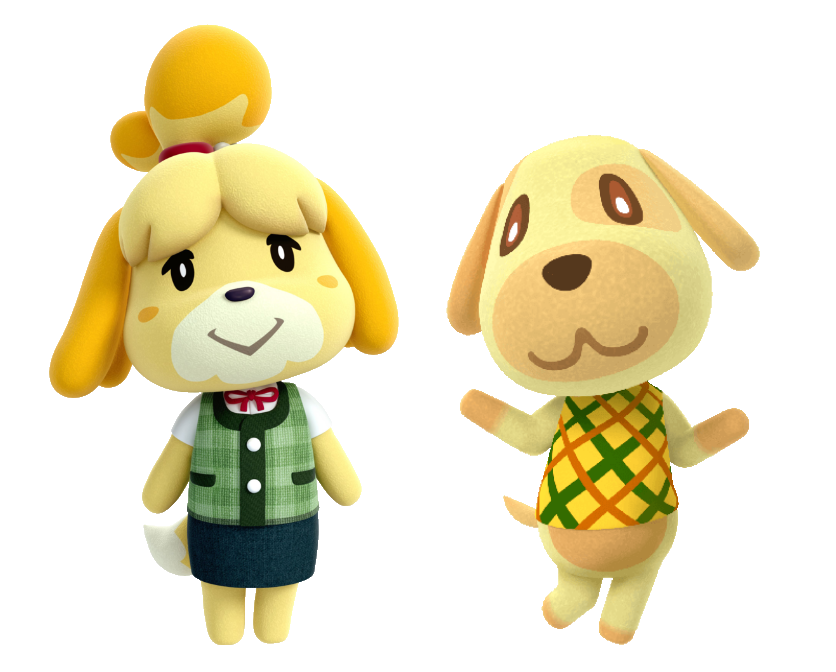
\includegraphics[width=10cm]{pictures/AnimalCrossing_merged.png}
    \end{figure}
    \vspace*{3cm}
    \textit{Merci pour tout.}
\end{center}

%%*******************************************************
% Declaration
%*******************************************************
\pdfbookmark[0]{Declaration}{declaration}
\chapter*{Declaration}
\thispagestyle{empty}

Put your declaration here.


%*******************************************************
% Table of Contents
%*******************************************************
\pdfbookmark[1]{\contentsname}{tableofcontents}

\setcounter{tocdepth}{2} % <-- 2 includes up to subsections in the ToC
\setcounter{secnumdepth}{3} % <-- 3 numbers up to subsubsections

\tableofcontents 

%*******************************************************
% List of Figures and of the Tables
%*******************************************************

%*******************************************************
% List of Figures
%*******************************************************    
\pdfbookmark[1]{\listfigurename}{lof}
\listoffigures

% %*******************************************************
% % List of Tables
% %*******************************************************
\pdfbookmark[1]{\listtablename}{lot}
\listoftables
  
%*******************************************************
% List of Listings
%******************************************************* 
%\pdfbookmark[1]{\lstlistlistingname}{lol}
%\lstlistoflistings 
   
%*******************************************************
% Acronyms
%*******************************************************
% \pdfbookmark[1]{Acronyms}{acronyms}
% \chapter*{Acronyms}
% \begin{acronym}[UML]
%     \acro{DRY}{Don't Repeat Yourself}
%     \acro{API}{Application Programming Interface}
%     \acro{UML}{Unified Modeling Language}
% \end{acronym} 

\part{Introduction}
\chapter{Cadre et contexte}  %Title of the First Chapter
Ce chapitre introduit le cadre de recherche de cette thèse, à la croisée des domaines de l'apprentissage humain du mouvement et des Environnements Informatiques pour l'Apprentissage Humain (EIAH). À l'issue d'une mise en contexte, les problématiques de recherche sont soulevées, et la contribution apportée est présentée.\\

L'apprentissage est un élément fondamental de l'humain. Notre capacité à observer, analyser, retenir et reproduire diverses choses nous permet de progresser tout au long de notre vie et de nous perfectionner. Cet apprentissage peut prendre plusieurs formes : formel / informel, par transmission orale, par imitation, mettant en jeu des connaissances tacites/explicites, \textit{etc.} \parencite{Eraut200Nfl}. Les récentes avancées technologiques font que l'informatique est maintenant profondément ancrée dans notre société. L'utilisation conjointe des possibilités offertes par l'informatique et du savoir et de l'expertise humaine dans les processus d'apprentissage permet la création d'environnements informatiques pour soutenir l'enseignement et l'apprentissage humain. En particulier, ces environnements peuvent s'appliquer à la formation aux gestes et aux mouvements.\\

Le mouvement humain peut être vu comme une succession de postures d'un corps dans l'espace, variant au cours du temps. Son apprentissage peut se faire de différentes manières : par imitation, c'est-à-dire la reproduction de chaque posture d'une personne experte démontrant le mouvement (p. ex. apprentissage de la danse), par acquisition des propriétés biomécaniques clés connues au préalable du geste cible (p. ex. coude en bas pour un lancer de pétanque, flexion puis extension des jambes vers l'avant et le haut permettant d'initier le service au tennis) ou par recherche des gestes permettant d'atteindre un état ciblé des objets manipulés par l'intermédiaire des mouvements à apprendre (opération chirurgicale nécessitant la manipulation d'un outil tel qu'un scalpel). L'apprentissage d'un geste peut poser plusieurs contraintes, en fonction du mouvement à effectuer : contraintes matérielles, d'espace, de mobilité, d'environnement, etc. l'objectif de cet apprentissage peut être multiple : caractère moteur (le mouvement) mais aussi un caractère fonctionnel (liée à l'objectif de l'action) ou caractère structurant (liées aux connaissances du sujet et du contexte d'apprentissage).

La capture des mouvements peut se faire à l'aide de nombreux dispositifs, tels que : les caméras RGB-D (\textit{Red Green Blue Depth}), popularisées grâce à l'apparition de systèmes grand publics abordables comme la Kinect de Microsoft, utilisable dans des contextes de recherche où les interactions gestuelles sont " simples " (c'est-à-dire quelques mouvements brefs sur un ensemble restreint d'articulations). Des combinaisons constituées de capteurs inertiels, telles que le Perception Neuron de NOITOM, proposent une capture intégrale du corps humain, tout en ayant un encombrement réduit. Pour des captures de haute précision, l'industrie du cinéma a souvent recours à des dispositifs de captation utilisant des caméras infrarouges, disposées autour de la scène, à l'aide d'une combinaison de marqueurs réfléchissants, portée par les acteurs. En fonction des besoins et du coût, et grâce au large choix des moyens de captation, il est possible d'obtenir des données de mouvements exploitables informatiquement et de construire des EIAH dédiés à leurs apprentissages.

La conception d'un environnement pour apprendre des mouvements nécessite de relever des défis propres aux domaines de l'étude des mouvements et de l'ingénierie des EIAH. Les prochaines sections sont dédiées à la définition des différents éléments constituant le domaine de recherche concerné par ce manuscrit, ainsi qu'à la problématique de la thèse et l'approche proposée.\\

\section{Environnements Informatiques pour l'Apprentissage Humain (EIAH)}
Les Environnements Informatiques pour l'Apprentissage Humain (EIAH) sont des environnements ayant pour but de favoriser l'apprentissage, en aidant, guidant et évaluant les apprenants d'une part et en assistant les enseignants d'autre part : que ce soit en présentiel, à distance, ou en situation mixte \parencite{Tchounikine2009PdR}. Une situation d'apprentissage impliquant un EIAH est en conséquence constituée d'au moins un artefact informatique, d'un enseignant (bien que la connaissance experte puisse être injectée dans l'EIAH), d'un apprenant, du matériel à manipuler (dans le contexte d'un apprentissage de gestes sportifs ou de gestes chirurgicaux par exemple), de l'environnement spécifique où a lieu l'apprentissage (p. ex. étude géologique sur le terrain), etc. Cependant, le point fondamental d'une situation d'apprentissage impliquant l'utilisation d'un EIAH est son aspect pédagogique. Ainsi, un EIAH doit être développé afin de servir et s'adapter à une ou plusieurs situations d'apprentissage. Autour des EIAH s'articulent plusieurs domaines de recherche : informatique, sciences de l'éducation, science de l'information et de la communication, didactique, psychologie, etc. Ces domaines sont complémentaires pour aboutir à la création d'un EIAH supportant de manière efficace le processus d'apprentissage. De plus, la fonction visée de l'EIAH (apprentissage théorique,  pratique, par imitation, sur une ou plusieurs séances, etc.) influe sur les compétences à mettre en œuvre pour son développement. La recherche en informatique sur les EIAH s'intéresse d'une part à la conception d'un tel système, mais également à son implémentation ainsi qu'à l'évaluation des impacts de son utilisation. Nous nous intéressons ici à l'accompagnement de l'expert, lors de sa tâche de transmission de savoir, et de l'apprenant dans sa tâche d'apprentissage. Les travaux présentés dans ce manuscrit n'ont pas vocation à remplacer l'expert lors de l'apprentissage, mais à l'assister dans la tâche d'observation, d'analyse et de retours donnés à l'apprenant.

\section{Le mouvement humain}
\subsection{Définition}
Le mouvement entendu comme le déplacement d'un corps dans l'espace à un moment donné, par rapport à un référentiel, est composé de variations à la fois spatiales et temporelles. Ce sont les différents paramètres de ces variations qui vont permettre de différencier un mouvement d'un autre, et leur donner une sémantique. En effet, le mouvement humain est porteur d'informations : il est possible d'extraire des informations bas-niveau, liées à la cinématique et la dynamique \parencite{Nunes2016}. Le geste est également porteur de sens dans le contexte de la communication verbale \parencite{Huang2015}, ou non-verbale \parencite{Chang201379}. En plus de cela, il est également possible d'inférer des informations de haut-niveau, par rapport à l'émotion \parencite{Kobayashi2007}, l'intention \parencite{Yu2015}, et l'action \parencite{Kapsouras20141432}.

\subsection{Méthodes d'apprentissage du mouvement}
Plusieurs méthodes d'apprentissage du mouvement existent. Une de ces méthodes est l'apprentissage par la reproduction du mouvement de l'expert. Dans ce cas, l'expert fait le mouvement cible, et l'apprenant s'applique à reproduire la succession de postures composant le mouvement. La décomposition du mouvement original en postures clés permet de fragmenter l'apprentissage du mouvement en plusieurs étapes successives, facilitant ainsi la reproduction du geste par l'apprenant \parencite{Maes2012DtM}.

Il est également possible d'apprendre le geste en acquérant les propriétés biomécaniques clés, connues au préalable, du geste cible. Cela nécessite d'être capable d'identifier, de qualifier voire de quantifier les différents paramètres (rotation, déplacement, durée, vitesse, etc.) des articulations ou des membres concernées par le mouvement. Dans ce cas, il faut être en mesure de pouvoir mesurer les propriétés du mouvement de l'apprenant, afin de les comparer avec les valeurs de références, soit spécifiées par l'expert \textit{a priori}, soit directement extraites du mouvement de ce dernier.

Enfin, lorsque l'objectif du geste est la manipulation d'un objet, l'apprentissage concerne la recherche des mouvements spécifiques (et leur optimisation) permettant d'atteindre l'état ciblé de l'objet. Un exemple d'un tel apprentissage est la manipulation d'outils chirurgicaux afin d'effectuer une opération. Dans ce cas, l'objectif est d'être capable d'effectuer le geste qui permet à l'outil d'arriver à la position et l'orientation désirée, ou d'être manipulé de la façon désirée, tout en prenant en compte les contraintes de manipulation propres au corps humain.

\subsection{Apprentissage de gestes avec des d'EIAH}
Les EIAH peuvent être conçus pour apprendre des gestes à des humains. Ces systèmes proposent différentes méthodes pour faciliter l'apprentissage du mouvement : un simple affichage du geste à effectuer et à reproduire, la manipulation d'un ou de plusieurs objets, l'immersion de l'apprenant dans un environnement en réalité augmentée, virtuelle ou mixte, etc.

L'affichage du mouvement à reproduire est une méthode analogue à l'apprentissage par reproduction du mouvement. Le support étant virtuel, il est possible de fournir un affichage superposé de l'apprenant avec celui du mouvement à effectuer \parencite{Kora20151559}, de proposer une comparaison avec un ou plusieurs experts \parencite{Yoshinaga2015Doa}, ou même de permettre à l'apprenant de visualiser quelles sont les différences entre son geste et celui de l'expert \parencite{Chan2011}. Il est possible de fournir une indication de performance quant au degré de similitude du geste de l'apprenant par rapport à celui de l'expert, soit à l'aide d'un score \parencite{Maes2012DtM}, soit à l'aide d'indications de positions directement sur le geste de l'apprenant \parencite{YAMAOKA2013912}.

Lors de la manipulation d'un objet, les systèmes peuvent contrôler non seulement la position de l'objet, mais également différents paramètres propres à la situation d'apprentissage (force appliquée, position du regard lors du mouvement, durée d'une partie spécifique du mouvement, etc.) \parencite{Chellali2016Aia}. Un retour visuel peut être donné à l'apprenant, en affichant la progression de la position et l'orientation de l'objet dans une scène en temps réel \parencite{Choi2015103}, mais il est également possible de donner des retours physiques, lors de l'utilisation de dispositifs tels que les bras haptiques \parencite{Gillespie2018Hit}. La mise en situation de l'apprenant dans un environnement virtuel pour la manipulation d'un objet permet de s'affranchir des contraintes imposées par les apprentissages classiques nécessitant un environnement spécifique.

Enfin, les systèmes utilisant les environnements virtuels permettent de renforcer l'engagement des apprenants dans la tâche à accomplir. Ces environnements peuvent par exemple être utilisés dans la rééducation post-attaque cardiaque, afin de faire réaliser les mouvements répétitifs au patient tout en proposant un contexte attrayant, réaliste \parencite{Baldominos2015AAt} ou ludique \parencite{Alankus2010TCG}.

La finalité d'un EIAH dédié à l'apprentissage de gestes étant la bonne réussite de ceux-ci, il est nécessaire de pouvoir analyser les données de mouvements de l'apprenant. L'analyse des données peut se faire de manière empirique par l'expert, ou de manière automatique par le système.

Lorsqu'il n'est pas possible de formaliser les caractéristiques qui font que le geste est considéré comme étant correct, l'analyse est faite de manière empirique. Dans le sport, les différences morphologiques font qu'il n'est pas toujours possible de proposer une comparaison pertinente avec les données de l'expert \parencite{Burns2011Uvh}, bien que des travaux pallient ces problèmes en utilisant plusieurs experts \parencite{Yoshinaga2015Doa}. Dans le domaine médical, l'analyse empirique de données de mouvements reste la méthode prédominante \parencite{Chen2016TPG, Wang2013HMM, Alankus2010TCG}, car l'expertise du médecin peut être difficile à formaliser sans être contextualisée en fonction du patient et de ses antécédents, ainsi que de la progression de la rééducation.

L'analyse automatique va permettre de proposer des retours sans l'intervention systématique d'un expert. Lorsque la connaissance experte est formalisable et quantifiable, il est possible de retourner à l'apprenant non seulement le degré de réussite de son geste \parencite{Maes2012DtM}, mais également des précisions quant aux différentes parties du mouvement \parencite{YAMAOKA2013912}. L'analyse des différences entre les gestes experts et ceux de l'apprenant permet également de mettre en lumière les caractéristiques déterminantes lors de la réalisation du geste en question \parencite{Makio2007DoS}. Il est même possible de découvrir quels sont les ensembles de règles implicites utilisées par des experts pour déterminer le degré de réussite d'un geste \parencite{Pirsiavash2014AQA}.

\subsection{Analyse automatique par méthodes d'apprentissage supervisé / non-supervisé}
Il existe d'ores et déjà des EIAH qui analysent automatiquement le mouvement à l'aide de techniques de \textit{Machine Learning}. Les algorithmes sous-jacents ont pour objectif d'apprendre à séparer des données, selon des critères variables. Ce domaine comprend plusieurs familles d'algorithmes : l'apprentissage supervisé, l'apprentissage non supervisé, l'apprentissage semi-supervisé et l'apprentissage par renforcement.

L'apprentissage supervisé est un terme qui regroupe un ensemble d'algorithmes permettant d'apprendre à une machine à classer des données sous la forme d'une fonction de séparation et de prédiction construite à partir d'une base de données annotées.

L'apprentissage non-supervisé cherche à découvrir une ou des structure(s) au sein des données non-étiquetées. Les regroupements obtenus n'ont pas de sémantique associée par l'algorithme, à l'inverse de l'apprentissage supervisé. Ces regroupements se font en fonction de propriétés communes entre les différentes données fournies en entrée de l'algorithme. Les critères d'évaluations de l'efficacité des regroupements obtenus se basent sur des critères de proximité des points au sein d'un même groupe et entre les groupes (distance intra-cluster vs distance inter-cluster) \parencite{Kassab2008Fbc}.

L'apprentissage semi-supervisé fait usage d'un petit nombre de données annotées. Les avantages sont multiples : l'utilisation d'un corpus de données annotées restreint limite le coût en temps d'annotation, il est possible de comparer les groupes obtenus avec les données étiquetées, permettant de juger de la répartition des données au sein des groupes, et il est possible de donner du sens aux groupes ainsi obtenus.

L'approche supervisée pour l'analyse de mouvement requiert un corpus suffisamment grand de données étiquetées pour chaque domaine et tâche ciblés. En pratique, le temps de capture et d'annotation n'est pas adapté à une utilisation \textit{in vivo}. Dans ce contexte, l'approche semi-supervisée ou non-supervisée est la plus adaptée. En effet, avec peu de données, l'utilisation de techniques de \textit{clustering} permet de :

\begin{itemize}
	\item regrouper les gestes en fonction des propriétés communes qui peuvent être spécifiées au préalable par l'enseignant,
	\item identifier les groupes de gestes acceptables en fonction de ces propriétés,
	\item positionner le geste de l'apprenant en termes de distance par rapport à ces groupes,
	\item suivre graphiquement l'évolution de ces propriétés individuellement ou conjointement.
\end{itemize}

Ces avantages combinés font que leur utilisation est pertinente dans le cadre d'une aide à l'apprentissage \textit{in vivo}. Cependant, il n'y a que peu de travaux qui font usage de tels algorithmes pour l'apprentissage de gestes. Ainsi, l'utilisation d'algorithmes de \textit{clustering} pour faciliter l'analyse et l'apprentissage de gestes est une piste explorée dans ce travail.

\subsection{Limites des systèmes existants}
Les EIAH permettant d'assister l'apprentissage du geste et d'analyser les données de mouvement sont souvent conçus de façon \textit{ad-hoc}, c'est-à-dire créés pour une situation d'apprentissage précise, dans un contexte fixé. Il est ainsi difficile, voire impossible, de réutiliser ces EIAH dans d'autres contextes sans un travail de réingénierie conséquent. Cela mène au développement de multiples EIAH dans des domaines pourtant analogues. De plus, l'intégration de la connaissance experte dans le système est souvent réalisée de manière fortement couplée, ce qui rend la généricité difficile. L'impossibilité d'introduire de nouveaux ensembles de règles pour une autre situation d'apprentissage fait que leur portée est limitée au domaine spécifique pour lequel ils ont été développés.

L'utilisation de techniques d'apprentissage supervisé pour l'analyse des gestes pose également le problème de la constitution d'un corpus spécifique pour la tâche concernée. Il n'est pas aisé de capturer, de segmenter et d'annoter un nombre de données suffisant pour qu'un tel algorithme puisse apprendre la fonction de séparation de manière correcte. En pratique, un système réutilisable dans différents contextes devra être en mesure de proposer des algorithmes d'apprentissage automatique pouvant travailler sur un nombre restreint de données, tout en permettant d'apporter une aide suffisante pour l'expert dans sa tâche d'analyse du geste, capturables par l'expert en amont de sa tâche d'enseignement : l'utilisation des algorithmes d'apprentissage supervisé n'est donc pas adapté à un EIAH dédié à l'apprentissage de gestes dans une situation \textit{in vivo}.

Enfin, dans le cas de l'apprentissage de mouvements, la présence d'un expert permet à l'apprenant de formuler des demandes précises en terme d'observation du geste à reproduire. Dans le cas d'un apprentissage à l'aide d'un EIAH dédié, les rôles de l'apprenant et l'enseignant ne sont pas toujours les mêmes en comparaison avec une situation d'apprentissage classique. Par exemple, certains systèmes écartent totalement l'expert du processus d'apprentissage. Bien que permettant un enseignement à distance, ou diffusé de manière plus large, il n'est pas possible pour l'apprenant de questionner l'expert sur des parties spécifiques du mouvement à effectuer. Il faut également que l'EIAH soit en mesure de prendre en compte des paramètres autres que le geste (morphologie, analyse fine des mouvements de l'apprenant, observations d'autres parties du corps pouvant mener à un geste incorrect, etc.), et donc que ces paramètres soient intégrés \textit{a priori} dans le système. En pratique, les données spécifiques « annexes » (c'est-à-dire non-spécifiques au geste à réaliser) à intégrer dépendent du contexte, mais également de l'appréciation de l'expert par rapport à l'apprenant et le geste à réaliser. Ainsi, les EIAH écartant l'expert du processus peuvent mener à un apprentissage moins efficace pour l'apprenant.

\section{Problématiques de recherche}
\subsection{Verrous scientifiques}
Dans le cadre de l'utilisation d'EIAH pour l'apprentissage de gestes, notre objectif est d'améliorer à la fois la situation d'apprentissage, tant pour l'enseignant que pour l'apprenant, mais également de faciliter la réutilisation d'un tel EIAH dans des contextes variés d'apprentissage de gestes.

Ainsi, un premier verrou réside dans l'analyse « fine »  des mouvements, en vue de leur reproduction ou de la détermination de leurs propriétés acceptables. Cette analyse constitue une tâche souvent fastidieuse, contextuelle à la tâche d'apprentissage et nécessitant des connaissances scientifiques solides en géométrie, physique et biomécanique. Le plus souvent, l'apprenant et l'enseignant ne possèdent pas de telles connaissances. Les méthodes automatiques d'analyse du mouvement utilisant l'approche supervisée ne sont pas utilisables dans une situation d'apprentissage \textit{in vivo}, car ils nécessitent un nombre de données étiquetées conséquent (de l'ordre du millier de données) et spécifique à la situation d'apprentissage considérée. De plus, les différences morphologiques entre les différents acteurs de l'apprentissage doivent être prises en compte si une analyse par superposition partielle ou totale des mouvements de l'expert et de l'apprenant est envisagée notamment.

Un moyen de résoudre ce problème est d'utiliser des descripteurs cinématiques du mouvement, ces derniers étant invariants à la morphologie. Une autre méthode pour pallier ce problème réside dans l'apprentissage par observation et reproduction du mouvement, à l'aide du EIAH dédié permettant de montrer le du geste de l'expert. Bien que l'étudiant puisse s'appuyer sur une telle représentation, les propriétés acceptables du geste ne seront pas nécessairement explicitement perçues ou identifiées. Cela constitue un deuxième verrou lié à la formalisation de l'expertise de l'enseignant qui doit être intégré au système formatif sous forme de règles ou de contraintes spatiales et temporelles. Il peut être difficile, voire impossible, pour un expert d'être en mesure d'expliciter de manière quantitative les observations qu'il réalise afin de juger le geste de l'apprenant.

Un troisième verrou est lié à la représentation intelligible d'indicateurs de progression contextuels et adaptés à l'apprentissage, dépendant de l'expertise, mais aussi des capacités de perception des acteurs. En effet, bien qu'il soit possible d'extraire de nombreuses informations à partir de données de mouvements capturés brutes, un système d'aide à l'apprentissage de mouvement doit être en mesure de proposer des indicateurs pertinents en fonction de la situation d'apprentissage considérée et des objectifs pédagogiques visés. La visualisation de ces indicateurs doit être adaptée non seulement à leur type (discret ou continu), leur sémantique mais également aux besoins d'observation et d'analyse de l'enseignant.

Le quatrième verrou est lié aux retours donnés à la suite de la réalisation du geste par l'apprenant. C'est cette étape qui permet à l'apprenant d'améliorer son geste. Si ce retour est fait par un EIAH, il faut être en mesure de déterminer en amont les propriétés qui font qu'un retour est pertinent pour l'apprentissage et la progression du geste de l'apprenant. Cette connaissance est parfois tacite pour l'expert. Ces paramètres peuvent donc varier en fonction de la situation d'apprentissage considérée, mais également de l'apprenant lui-même. De plus, un système réutilisable et adaptable dans d'autres contextes faisant intervenir le mouvement ne doit pas nécessiter un processus de réingénierie lourd.

\subsection{Questions de recherche}
Le développement d'EIAH support à l'enseignement de gestes, extensibles au-delà de la tâche pour laquelle elles ont été conçues et ayant un coût minimal en termes de réingénierie, représente un défi qui soulève plusieurs questions de recherche :

\begin{itemize}
\item \textbf{Q1} : Comment développer un système permettant de caractériser le geste à l'aide de l'intégration de l'expertise d'un enseignant ?
\item \textbf{Q2} : Comment évaluer et comparer le geste (ou ses propriétés) de l'apprenant avec celui de l'enseignant afin d'évaluer la progression de l'apprentissage ?
\item \textbf{Q3} : Comment, dans une situation d'apprentissage de gestes donnée, proposer des retours pertinents et compréhensibles aux acteurs de l'apprentissage non spécialistes en analyse du mouvement ?
\end{itemize}

\subsection{Hypothèses de recherche}
À partir des éléments précédemment expliqués, ainsi que des questions de recherches formulées, six hypothèses seront vérifiées dans ces travaux :
\begin{itemize}
	\item \textbf{H1} : Il est possible de regrouper les gestes selon leurs propriétés cinématiques communes. (\textbf{Q2})
	\item \textbf{H2} : Il est possible de séparer les gestes des apprenants en deux groupes correspondant à une dichotomie geste réussi / geste raté afin de déterminer, pour une situation d'apprentissage donnée, les propriétés d'un ensemble fini de gestes réussis. (\textbf{Q1})
	\item \textbf{H3} : Il est possible de séparer les gestes en fonction de propriétés attendues et identifiées au préalable par l'expert. (\textbf{Q1})
	\item \textbf{H4} : Il est possible de corriger chaque défaut du geste de l'apprenant, en lui indiquant les défauts majeurs à corriger en premier. Un défaut majeur est identifié par la plus grande distance séparant le mouvement courant de l'apprenant, du groupe de gestes acceptables ayant éliminé ce défaut. (\textbf{Q2})
	\item \textbf{H5} : L'utilisation du système MLA basée sur l'hypothèse 4 permet d'améliorer l'apprentissage du geste par rapport à une situation sans le système MLA. (\textbf{Q3})
	\item \textbf{H6} : L'utilisation du système MLA en tant qu'assistant à l'enseignant permet d'améliorer l'apprentissage du geste par rapport à une situation sans MLA, et à une situation avec MLA et sans enseignant. (\textbf{Q3})
\end{itemize}

La validation ou non de ces hypothèses s'effectuera à travers le système d'aide à l'apprentissage de mouvements développé au cours de cette thèse.

\section{Aperçu des contributions}
\subsection{Motion learning Analytics (MLA)}
Afin de répondre à ces questions, notre approche s'est axée autour du système \textit{Motion Learning Analytics} (MLA), développé pour les besoins de cette thèse. Il s'agit d'un système d'analyse de mouvement, combinant la captation, le filtrage, le traitement et l'analyse (à l'aide de méthodes d'apprentissage non-supervisé ou semi-supervisé) du mouvement. L'approche consiste à traiter des données de mouvement brutes, afin de les rendre : (i) exploitables, en éliminant les défauts inhérents au système de capture utilisé et (ii), compréhensibles, en extrayant des descripteurs de mouvement à partir des données filtrées. Une fois ces étapes réalisées, l'objectif du système est alors double : (i) proposer automatiquement une évaluation et des conseils pour l'amélioration du geste de l'apprenant à partir de la comparaison de propriétés du mouvement de l'apprenant avec celles attendues et calculées à partir des mouvements de l'expert, et (ii) proposer un affichage graphique de la progression de l'apprenant, en fonction des défauts considérés, sur lequel peut s'appuyer l'expert.

Cette plateforme a permis de valider notre approche, et d'apporter ainsi une preuve de concept de notre chaîne allant de l'acquisition du mouvement jusqu'à l'analyse de ces derniers :

\begin{itemize}
    \item L'acquisition du mouvement se fait à l'aide du Perception Neuron, une combinaison constituée de multiples capteurs inertiels, permettant de capturer le mouvement en temps réel.
    \item Les données exportées au format BVH sont passées dans une chaîne de traitements, afin d'améliorer le signal. Les données sont ensuite utilisées afin de calculer des descripteurs, correspondant à des aspects spécifiques du mouvement (vitesse, accélération, etc.).
    \item Les descripteurs sont utilisés dans un processus de \textit{clustering}, afin d'étudier la séparation possible des gestes, selon leur degré de réussite, leurs défauts ou les propriétés d'acceptabilité identifiées en amont par un expert.
    \item Les données de l'apprenant sont comparées à celles de l'expert, afin de déterminer quels sont les conseils à donner à l'apprenant afin qu'il améliore son geste.
\end{itemize}

\subsection{Traitement et segmentation des mouvements}
La chaine de traitement des données permet non seulement de filtrer les artéfacts propres aux données obtenues à partir du Perception Neuron, mais également de n'en garder que la partie jugée utile à l'aide d'un algorithme de segmentation et d'en extraire des descripteurs jugés pertinents dans la situation d'apprentissage concernée.

\subsection{Séparation des données de mouvement et sémantique associée}
L'utilisation d'algorithmes de \textit{clustering} permet non seulement de travailler avec un nombre restreint de données, mais également de proposer un regroupement des données en fonction de propriétés définies au préalable par l'expert. L'ajout d'un petit nombre de données étiquetées permet de donner un sens aux groupements obtenus, permettant une comparaison des données de l'apprenant par rapport aux gestes jugés bons ou mauvais.

\subsection{Système de retour visuel}
Enfin, un système de retour visuel, permettant à l'utilisateur de juger de la distance des données de l'apprenant par rapport à celles de l'expert, permet de consolider l'avis de l'expert ou de donner des pistes quant aux défauts les plus significatifs du geste de l'apprenant, dans le cas où le jugement est difficile.

\section{Expérimentations}
Le système a été testé au travers de trois expérimentations, permettant chacune de tester les hypothèses présentées dans cette introduction. Ces trois expérimentations consistent en la réalisation de gestes dont deux exigent une certaine technicité, puis à l'utilisation de ces données pour tester les hypothèses. La première expérimentation consistait à lancer une balle dans deux corbeilles éloignées l'une de l'autre. L'objectif ici était de voir s'il était possible d'obtenir une séparation acceptable du geste en fonction d'une ou plusieurs propriétés définies au préalable, correspondant à différentes stratégies de lancers. Une séparation correspondant au type de lancer a été obtenue. Le geste de la deuxième expérimentation était celui du \textit{Bottle Flip Challenge}, où il faut lancer une bouteille tout en lui imprimant une rotation sur son axe horizontal, puis la faire retomber debout sur une surface plane. Les données de cette expérimentation ont été utilisées afin de vérifier s'il était possible de séparer les gestes en deux groupes correspondant aux gestes réussis et ceux ratés. Il a été possible d'obtenir une bonne séparation mais pas une séparation en fonction des groupes considérés. Enfin, la troisième expérimentation s'est appuyée sur le lancer de fléchettes comme domaine applicatif, afin de tester la pertinence du système MLA en tant qu'outil de regroupements des gestes suivant des propriétés identifiées en amont par un expert, et en tant qu'outil de retours à l'apprenant et d'assistance à l'enseignant.

\section{Plan du manuscrit}
Le chapitre suivant porte sur un état de l'art des EIAH dédiés à l'apprentissage du geste. Y sont introduit les différentes modalités utilisées au sein de ces EIAH : objectif du système, données utilisées et leur représentation informatique, méthodes de captation, analyses effectuées, retours fournis à l'apprenant et place de l'expert dans le processus.\\

Le chapitre trois propose une étude bibliographique des informations extractibles du mouvement, appelées descripteurs du mouvement. Ces descripteurs permettent de caractériser le mouvement afin de pouvoir l'analyser en fonction des besoins d'observations ou des propriétés cinématique du mouvement. Une analyse bibliographique des différents descripteurs, ainsi que de leur utilisation dans des contextes de recherche sur le mouvement est réalisée. Un tableau présentant des descripteurs couvrant un ensemble de propriétés observables est proposé à la fin de ce chapitre.\\

Le chapitre quatre se concentre sur les méthodes d'analyses appliquées à des mouvements capturés. À partir des descripteurs calculés, il est possible de réaliser des analyses précises sur le mouvement, soit par un expert, soit par un processus automatique. Ce chapitre présente ces analyses sous deux angles majeurs : l'analyse empirique qualitative et l'analyse automatique quantitative.\\

Le chapitre cinq présente la contribution apportée au travers du système MLA, développé pour l'aide à l'évaluation de gestes humains. Y sont présentées les différentes étapes, du traitement des données des mouvements brutes jusqu'à l'aide proposée à l'expert et aux apprenants.\\

Le chapitre six est dédié aux trois expérimentations qui ont permis de tester les hypothèses de recherche.\\

Pour terminer, le dernier chapitre fournit un résumé des apports de cette thèse, et ouvre plusieurs pistes et perspectives de recherche.



 %!TEX root = ../thesis.tex
%*******************************************************************************
%****************************** Second Chapter *********************************
%*******************************************************************************
\part{État de l'art}
\chapter{Les EIAH pour l'apprentissage de gestes}
Ce chapitre présente un état de l'art sur les différents éléments nécessaires à la conception d'EIAH pour soutenir l'apprentissage humain de gestes. La première partie rappelle et décrit l'une des représentations informatiques les plus connues pour modéliser le mouvement humain i.e. la représentation par une succession temporelle de squelettes. La seconde partie fait état des différents moyens pour capturer le mouvement. La troisième partie se concentre sur les EIAH existants, le matériel utilisé pour la capture, leurs principales caractéristiques (\textit{e.g.} domaines applicatifs, types de données utilisées, etc.) et les retours faits à l'apprenant. De plus, elle étudie ces systèmes sous l'angle de la réingénierie et la place/le rôle des usagers au sein de ces systèmes.

%REFAIRE L'INTRO (obviously)

Dans la suite de ce manuscrit, nous utiliserons le terme de « geste cible », pour faire référence au geste à apprendre pour atteindre l'objectif de la tâche à réaliser. En effet, il existe parfois, pour une même tâche d'apprentissage, plusieurs gestes possibles jugés corrects par un ou plusieurs experts. Ces gestes constituent l’objectif d’apprentissage. Si l'on prend l'exemple du service au tennis, et que l'on définit la tâche comme étant le fait de frapper la balle de manière à ce qu'elle arrive dans la zone légale de service adverse, plusieurs mouvements existent : le lancer " droit ", le lancer " arrière " et le lancer " devant ". De plus, il est possible d'imprimer un effet à la balle lors de la frappe (\textit{lifté} ou \textit{slicé}), ce qui induit une variation du geste de frappe \parencite{Zappala2017IoP}. Au bowling, il existe à minima trois types de lancers différents (\textit{Stroker}, \textit{Cranker}, \textit{Spinner}) pour atteindre l'objectif, qui est de renverser un maximum de quilles en un minimum de lancers  \parencite{Tan2000Cbp}. Ces deux exemples parmi tant d'autres montrent qu'il ne serait possible de définir un seul geste comme étant le geste parfait à atteindre pour une situation d'apprentissage donnée. En conséquence, nous introduisons le terme de " geste cible ", qui est le geste dont les caractéristiques sont : (i) connues par l'expert et (ii) doivent être transmises à, et maîtrisées par, l'apprenant. Le geste cible peut être différent d'un expert à l'autre pour un mouvement donné, en fonction de l'objectif recherché et des spécificités morphologiques.

%DANSE : \parencite{Maes2012DtM} (a mettre dans le tableau)

\section{Représentation du mouvement}
Afin de pouvoir exploiter les données de mouvement au sein d'un EIAH, il faut pouvoir formaliser, discrétiser puis opérationnaliser les mouvements du corps. Une des techniques les plus utilisées consiste à utiliser des graphes, et plus particulièrement des arbres, afin de modéliser les mouvements du corps humain sous la forme d'une succession de squelettes 3D, c'est-à-dire des postures espacées selon un pas de temps fixe ou variable \parencite{Lewis2000Psd}.

Le corps humain peut ainsi être vu comme un ensemble structuré d'articulations sous la forme d'une arborescence (Fig. \ref{fig:3D_skeleton_tree_example}). Dans ce cas, les nœuds de l'arbre représentent les articulations, et les arcs représentent les différents membres du corps.

\begin{figure}[h]
    \centering
    \includegraphics[width=5cm]{pictures/3D_skeleton_tree_example.png}
    \caption[Représentation informatique d'un squelette humain en 3D]{Un exemple de squelette humain 3D représenté sous la forme d'un arbre. Les articulations sont représentées à l'aide de nœuds (en vert), et les membres du corps sont les arcs reliant ces nœuds entre eux (en bleu).}
    \label{fig:3D_skeleton_tree_example}
\end{figure}

Chaque nœud contient généralement plusieurs informations : le nom, la position et/ou l'orientation de l'articulation, ainsi que des références vers les articulations parentes et filles. L'articulation racine généralement choisie dans le cadre d'un squelette est celle des hanches, car située près du centre de masse du corps humain. On définit également souvent sa position comme étant l'origine  $(0,0,0)$ du repère tridimensionnel cartésien (Fig. \ref{fig:skeleton_pos_ori_example}). Les systèmes de captures usuels ne peuvent capter qu'une fraction des éléments constituants le corps humain : un corps humain est composé d'environ 360 articulations, 206 os et 640 muscles. L'ensemble de ces éléments ne sont pas nécessairement modélisés pour étudier les mouvements humains suivants le contexte. Ainsi, pour caractériser le mouvement d'une personne s'asseyant, la variation sur l'axe vertical du centre de masse, ou encore la position de la projection du centre de masse par rapport au support du corps (les pieds) sera suffisante \parencite{Salamah2015HMf}.

\begin{figure}
    \centering
    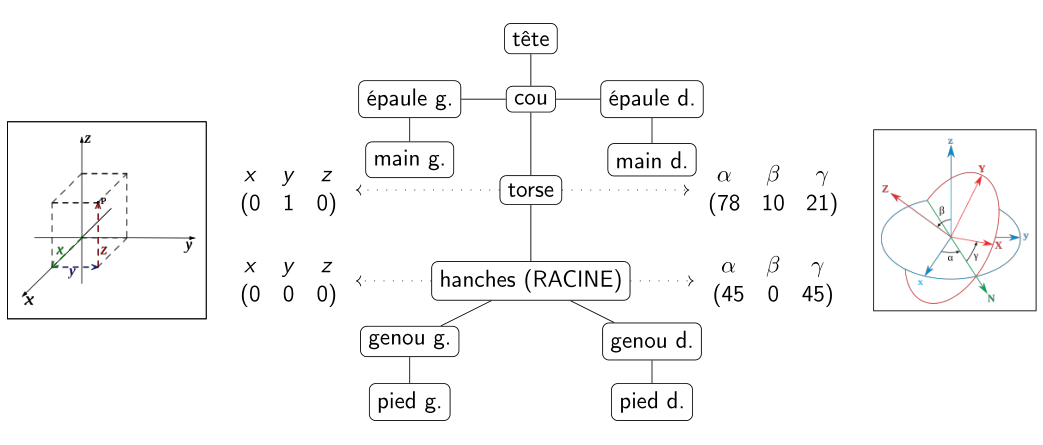
\includegraphics[width=\textwidth]{pictures/skeleton_pos_ori_example.png}
    \caption[Données d'un squelette 3D]{Un exemple de squelette humain représenté sous forme informatique avec, pour chaque articulation, des informations de position et d'orientation relatives à l'articulation parente.}
    \label{fig:skeleton_pos_ori_example}
\end{figure}

Cette structure est particulièrement adaptée pour modéliser tout ou une partie du corps. La représentation du corps humain sous forme de chaîne articulaire 3D, afin de représenter un mouvement, sera celle utilisée dans la suite de ce manuscrit.

% Il existe d'autres représentations pour un corps humain, telle que celle proposée par \parencite{Kulpa2005Mir} : dans ce cas, certains segments du corps sélectionnés sont stockés sous une forme normalisée, ainsi que les plans contenant les articulations intermédiaires non conservées. Cette approche permet une certaine liberté quant à l'adaptation du squelette initial à une autre morphologie, tout en conservant une représentation proche de la réalité du mouvement d'origine. [JUSTIFIER VOIR CORRECTIONS] Seules les données de mouvement représentées sous forme de chaîne articulaires 3D seront considérées dans la suite de ce manuscrit.

Afin d'obtenir un mouvement représenté sous forme d'un arbre, et ainsi exploitable à l'aide d'outils informatiques, il faut être en mesure de le capturer. La capture de mouvements peut être réalisée à partir de plusieurs dispositifs, permettant soit d'obtenir des données 2D (\textit{i.e.} images ou vidéos), ou directement des données 3D (squelette de la personne, nuage de points, modèles surfaciques, \textit{etc.}). En fonction du matériel de capture utilisé, le processus d'acquisition, ainsi que les contraintes associées, la qualité des données obtenues ne sera pas la même. Le choix d'un dispositif de capture adapté à un contexte d'apprentissage de geste doit se faire en fonction des besoins d'observation et d'analyse du geste, tout en prenant en compte les contraintes imposées par la réalisation du geste : amplitude, parties du corps impliquées, manipulation d'objet, environnement spécifique, \textit{etc.}.

\section{Matériel de capture et données obtenues}
Il est possible de séparer l'apprentissage de gestes en deux grandes familles non exclusives : les cas où le geste est la finalité de l'apprentissage, et le cas où la manipulation d'un objet est l'objectif final. Dans le premier cas, le corps humain (une partie ou dans son entièreté) va être au cœur de l'analyse, alors que dans le deuxième cas, la position de l'objet, et parfois le geste permettant d'y arriver seront les points d'intérêt principaux. Les dispositifs utilisés sont ainsi choisis en fonction de l'objet considéré pour la captation (\textit{i.e.} le corps ou un objet), mais aussi du rapport coût/caractéristiques souhaités de l'équipement, déduits de la situation d'apprentissage et des besoins d'observation. En termes de caractéristiques, l'encombrement, l'espace de travail, la chaine de traitements des données et leur précision, ainsi que les retours sensoriels souhaités du système (visuels et/ou haptiques) sont souvent considérés pour ce choix \parencite{Chamaret2010}. Cette section s'intéresse d'abord aux dispositifs dédiés à la capture d'un corps humain, puis aux dispositifs dédiés à la simulation ou la capture de position et d'orientation d'objets. Les coûts de ces dispositifs peuvent être très importants, mais il est maintenant possible d'obtenir des données de mouvements capturés d'une qualité suffisante pour effectuer des analyses de geste d'apprenant à partir de systèmes relativement peu onéreux. Cet aspect \textit{low/middle-cost} de la captation de mouvement est intéressant pour des captures prenant place dans des situations variées (par opposition à la captation dans un environnement dédié, par exemple en laboratoire), ce qui en fait le choix retenu pour cette thèse.

Dans des domaines tels que le sport \parencite{YAMAOKA2013912} (lancer de disque) \parencite{Yoshinaga2015Doa} (archérie) \parencite{Chan2011} (danse), le corps entier de l'apprenant va être capturé et utilisé. Dans ces cas-ci, l'analyse va concerner le mouvement d'une partie ou du corps entier. Il est possible d'obtenir ces données à partir de vidéos, de caméras RGB-D (\textit{Red Green Blue Depth}) \parencite{Yoshinaga2015Doa} \parencite{Kora20151559} \parencite{YAMAOKA2013912}, d'un ensemble de capteurs réduit placés à des endroits spécifiques du corps \parencite{PORCIUNCULA2018S220} ou d'une combinaison de capteurs \parencite{Chang201379}.

\subsection{Extraction de mouvement par vidéo}
Il est possible d'extraire des données de mouvement à l'aide de vidéos. Ces méthodes reposent sur l'inférence du mouvement à partir d'un ensemble de pixels \parencite{Lv2015CEI}. Il existe une multitude de techniques, et certaines d'entre elles permettent d'obtenir un squelette 3D. Une revue des principales méthodes utilisées est proposée dans \parencite{Sarafianos2016DHp} : projection dans un espace 2D de données de mouvement 3D, afin d'obtenir une correspondance avec l'image / la vidéo, utilisation de contraintes rigides sur plusieurs images successives afin de retrouver le squelette le plus probable, \textit{etc.} Il est également possible d'utiliser des vidéos stéréos, permettant ainsi d'obtenir des points de repère dans l'espace et de faciliter le suivi de points spécifiques du corps, afin de reconstituer un squelette 3D correspondant au mouvement (Fig. \ref{fig:stereo_video_skeleton}) \parencite{Liu2016Tb3}.

\begin{figure}[h]
    \centering
    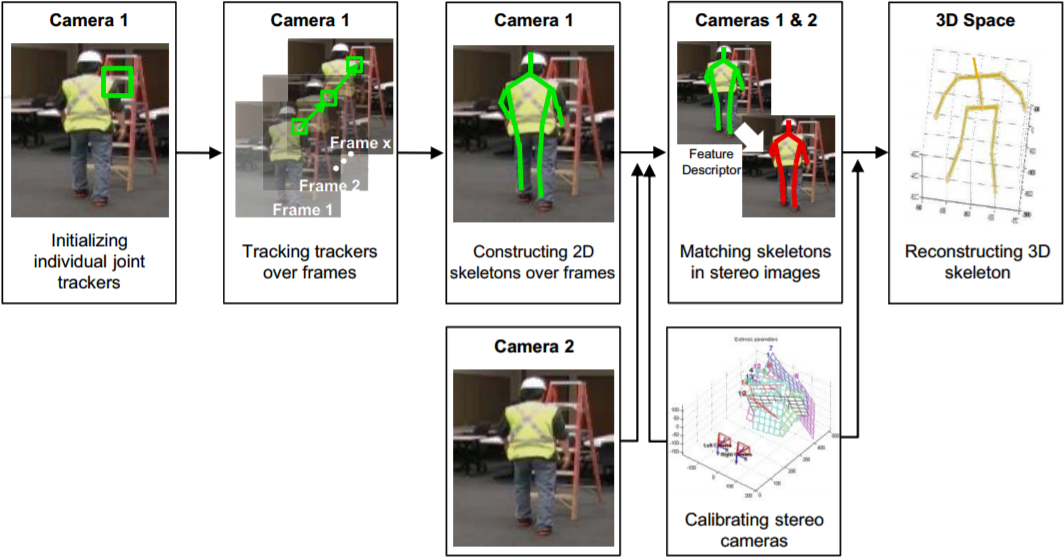
\includegraphics[width=10cm]{pictures/stereo_video_skeleton.png}
    \caption[Squelette reconstitué à partir de vidéo stéréo \parencite{Liu2016Tb3}]{Le squelette 3D peut être reconstitué à partir de vidéo stéréo \parencite{Liu2016Tb3}.}
    \label{fig:stereo_video_skeleton}
\end{figure}


\subsection{Extraction de mouvement par vidéo et capteur de profondeur}
Les caméras RGB-D sont des dispositifs de capture se basant sur la combinaison d'une capture vidéo 2D et d'un mapping de profondeur sur chaque pixel, généralement obtenu à l'aide d'un capteur infrarouge. L'ajout de l'information de profondeur à la vidéo 2D permet d'obtenir une information supplémentaire notamment sur le déplacement des acteurs dans la scène filmée. Leur encombrement relativement réduit, combiné à la non nécessité d’avoir des marqueurs équipés sur le corps font que ces dispositifs ont été largement utilisés dans des contextes de recherche tels que : la capture en temps réel de multiples personnes \parencite{Basso2013}, la reconstruction de scènes interactives en 3D \parencite{Izadi11kinectfusion} ou encore la capture du mouvement \parencite{Yoshinaga2015Doa}. En effet, il est possible d'obtenir le squelette d'une personne à l'aide des outils fournis par les entreprises développant ces caméras (Fig.\ref{fig:skeleton_kinectv2}) : jusqu'à 6 squelettes de 20 articulations chacun peuvent être capturés simultanément (25 articulations par squelette pour la Kinect v2, voir Fig. \ref{fig:skeleton_kinectv2}). La précision de la Kinect permet de capter les pouces de chaque main, mais pas les doigts pris individuellement.\\

\begin{figure}
    \centering
    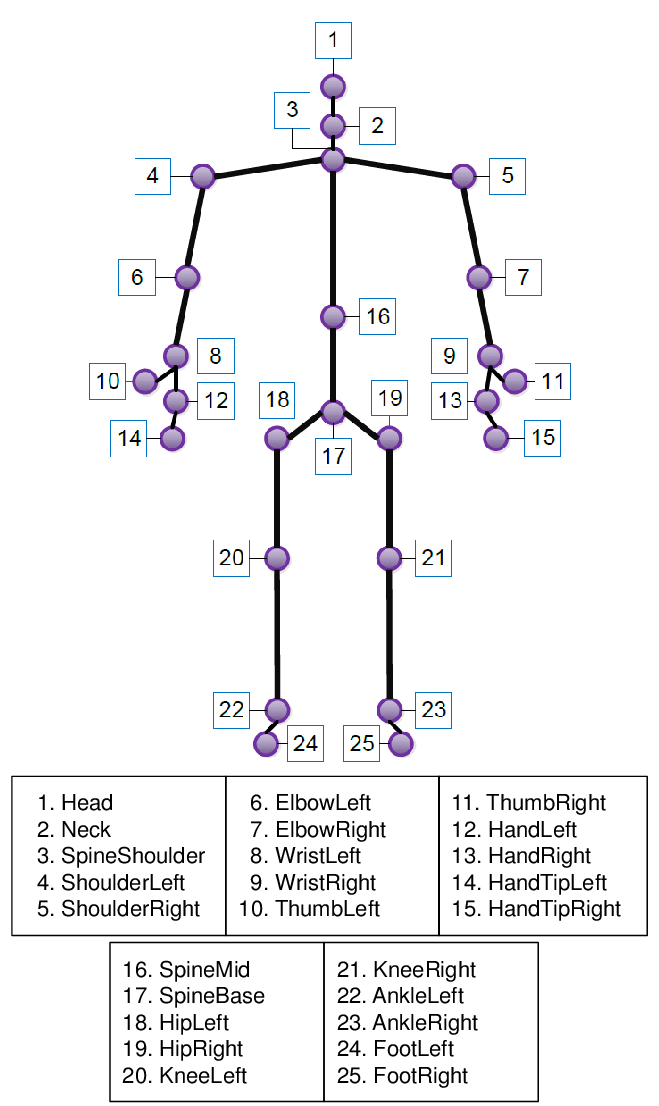
\includegraphics[width=5cm]{pictures/3D-skeleton-joints-tracked-by-the-Kinect-v2-sensor.png}
    \caption[Squelette et articulations captés par la Kinect V2 \parencite{Faisal2015Kinect}]{Squelette et articulations captés par la Kinect V2 \parencite{Faisal2015Kinect}. Le nombre d'articulation est suffisant pour pouvoir représenter les changement de position et d'orientation de tous les membres du corps humain.}
    \label{fig:skeleton_kinectv2}
\end{figure}


Les caméras RGB-D possèdent cependant des inconvénients. En effet, le problème de l'occlusion est fréquent. Il apparaît dès lors qu'une partie du corps est masquée par une autre, par rapport à l'objectif de la caméra. Il est possible de pallier ce problème grâce à l'utilisation de plusieurs caméras en simultanées (Fig. \ref{fig:multiple_rgb_d_camera_system}), et dont les différentes images sont utilisées pour reconstruire le squelette final \parencite{Regazzoni2014Rcv}. Cette méthode nécessite un calibrage très précis, ainsi qu'un environnement dédié à la captation des mouvements.\\

\begin{figure}[h]
    \centering
    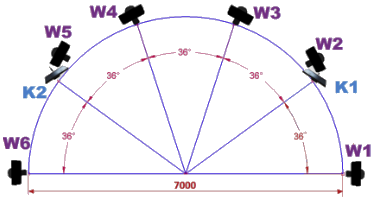
\includegraphics[width=7.5cm]{pictures/multiple_rgb_d_camera_system.png}
    \caption[utilisation de multiples caméras RGB et RGB-B pour éviter l'occlusion \parencite{Regazzoni2014Rcv}]{L'utilisation de plusieurs caméras RGB, ainsi que RGB-D permet d'éviter les problèmes d'occlusion \parencite{Regazzoni2014Rcv}.}
    \label{fig:multiple_rgb_d_camera_system}
\end{figure}

\subsection{Extraction de mouvement par caméra infrarouge}
La méthode la plus précise, en termes de qualité des données, pour capturer un corps entier à l'heure actuelle est celle basée sur les caméras infrarouges utilisées conjointement avec des marqueurs réfléchissants (Fig. \ref{fig:infrared_camera_Morel}). Ces systèmes sont les plus précis pour l'acquisition de mouvements d'une ou plusieurs personnes en simultané \parencite{Pfister2014Cao} \parencite{Yang2016HUL}. Ils sont très utilisés dans l'industrie du cinéma et du jeu vidéo, afin de proposer des mouvements les plus fidèles possibles. Les inconvénients majeurs de ces systèmes sont d'une part le coût (chiffré en plusieurs centaines de milliers d'euros pour un système basé sur 8 caméras), la non portabilité du matériel de capture (nécessité d'avoir un emplacement dédié et fixe) et la chaine lourde de traitements pour reconstituer le squelette 3D (\textit{e.g.} capture des points, filtrage pour la réduction des phénomènes occlusions, reconstitution de la chaîne articulaire et des orientations de chaque articulation). Bien que des entreprises proposent des solutions tout-en-un pour obtenir le squelette 3D d'un ou plusieurs acteurs (\textit{e.g.} Qualysis, Vicon, Optirak), ils nécessitent les compétences d'un informaticien qualifié pour être utilisé. En effet, le placement des capteurs doit se faire de manière optimale (soit en suivant les recommandations fournies par les fabricants des systèmes utilisés, soit en fonction des besoins de captation) afin de s'assurer que les marqueurs réfléchissants soient visibles par au moins une caméra afin de limiter au maximum les phénomènes d'occultation, et les données doivent ensuite être filtrées à l'aide des logiciels fournis par les fabricants ou en utilisant des logiciels externes. Ces filtres peuvent avoir plusieurs objectifs : ré-interpolation du mouvement à une fréquence plus ou moins rapide, lissage des données de mouvement et d'orientation par moyennage des postures proches, effacement des pics de valeurs en fonction des valeurs voisines, \textit{etc.}

\begin{figure}[h]
    \centering
    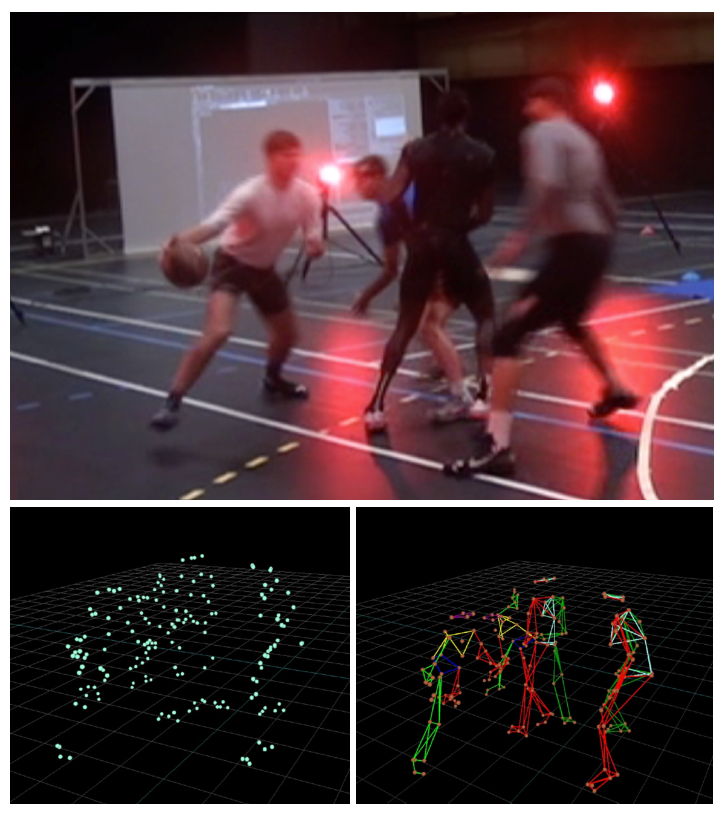
\includegraphics[width=10cm]{pictures/infrared_camera_Morel.png}
    \caption[Système de captation par caméra infrarouge \parencite{Morel2017Mts}]{Un système de captation à base de caméras infrarouges et de marqueurs disposés sur le corps (eu haut). Les données sont obtenues sont la forme d'un nuage de point (en bas à gauche), à partir desquels les squelettes sont reconstitués (en bas à droite) \parencite{Morel2017Mts}.}
    \label{fig:infrared_camera_Morel}
\end{figure}

\subsection{Extraction de mouvement par capteurs inertiels portables}
L'utilisation de capteurs portés par le corps représente une autre méthode pour enregistrer les mouvements. Ces capteurs sont généralement reliés entre eux, et permettent de transmettre les données par une liaison filaire ou sans fil, se libérant ainsi des contraintes de l'espace fixe \parencite{PORCIUNCULA2018S220}. Un capteur renferme un ou plusieurs dispositifs de mesure tels que : un accéléromètre, permettant de mesurer l'accélération linéaire, un gyromètre, permettant de mesurer la vitesse angulaire, et un magnétomètre, qui permet de mesurer la force et la direction d'un champ magnétique. La combinaison de ces trois informations permet de déduire les positions et orientations d'un corps en mouvement dans l'espace. Ainsi, il est possible d'obtenir des données de mouvements dans des contextes plus variés que les systèmes nécessitant une installation fixe. Afin de permettre l'acquisition d'un squelette humain, il est possible de combiner plusieurs de ces capteurs, posés sur plusieurs parties du corps (au niveau des articulations).

Cependant, les données obtenues peuvent être moins précises qu'avec des systèmes fixes (\textit{e.g.} perturbations liées à l'environnement, qualité de transmission des données variable, \textit{etc.}). Un des problèmes souvent rencontrés est celui de la dérive. Il s'agit de la variation des données renvoyées par un capteur, sans que cette variation ne soit le résultat d'un changement de position ou d'orientation réel. Bien que des méthodes existent pour corriger ces défauts, cela implique généralement d'utiliser d'autres types de données pour compenser les erreurs propres au matériel (données GPS, par exemple \parencite{Bevly2004Gps}). Cependant, en fonction du degré de précision nécessaire, ces méthodes ne sont pas toujours adaptées et réutilisables dans tous les contextes. Ainsi, il est parfois nécessaire de disposer d'une chaîne de traitements adaptée afin d'éliminer ces erreurs. Ainsi, une technique de filtrage des données proposée par Roetenberg \textit{et al.} est celle basée sur un filtre de Kalman, fusionnant plusieurs informations provenant de capteurs différents (gyroscopes, accéléromètres, magnetomètres) afin d'estimer l'erreur et ainsi la corriger à la volée  \parencite{Roetenberg2005Com}. Les casques de réalité virtuelle récents font également usage de capteurs inertiels (disposés sur le casque lui-même) afin de proposer une plus grande immersion dans les jeux, en rajoutant le mouvement comme interaction,. L'ajout de ces capteurs inertiels permet également de réduire les problèmes de nausées propres à ces casques \parencite{HTCViveSpecs}.

\subsection{Matériel de captation pour la manipulation d'objets}
Dans le cas où la manipulation de l'objet est au cœur de l'apprentissage, bien que le geste soit parfois important, l'état de l'objet (position, orientation, intégrité, \textit{etc.}) est l'objectif de l'apprentissage du geste, et donc de la captation. Cette différence se retrouve notamment au niveau des données capturées et utilisées : dans les domaines tels que la chirurgie \parencite{BMT_2015} \parencite{Choi2015103} ou la musique \parencite{Ng2008}, la position de l'objet est souvent la donnée de mouvement principale récupérée pendant la tâche (possiblement utilisée conjointement avec d'autres informations, telles que la position du regard \parencite{BMT_2015}). Ces données peuvent être capturées à l'aide de dispositifs adaptés : les interfaces haptiques en sont un exemple (Fig. \ref{fig:haptic_arm}).

Ces interfaces permettent non seulement une manipulation plus aisée d'un objet virtuel, mais également un retour sensitif au niveau du toucher lors de la manipulation \parencite{SREELAKSHMI20174182}. Ainsi, il est possible d'obtenir des retours de force ou tactile permettant d'émuler respectivement la forme ou la texture d'un objet. En combinant ces retours à des environnements de réalité virtuelle, il est possible de proposer une sensation de saisie, de collision et de toucher, en conjonction avec ce qui est visuellement présenté à l'utilisateur \parencite{Whitmire2018}. Ce dispositif est très utilisé dans le cadre de l'apprentissage de manipulation d'objets médicaux, tels que pour l'insertion d'aiguilles sous la peau \parencite{CORREA20196}, la manipulation de sondes \parencite{Choi2015103}, le cathétérisme \parencite{PEPLEY20171066}, ou encore l'entrainement du personnel à la planification pré-opératoire par télé-chirurgie \parencite{HALABI20189}.

\begin{figure}
    \centering
    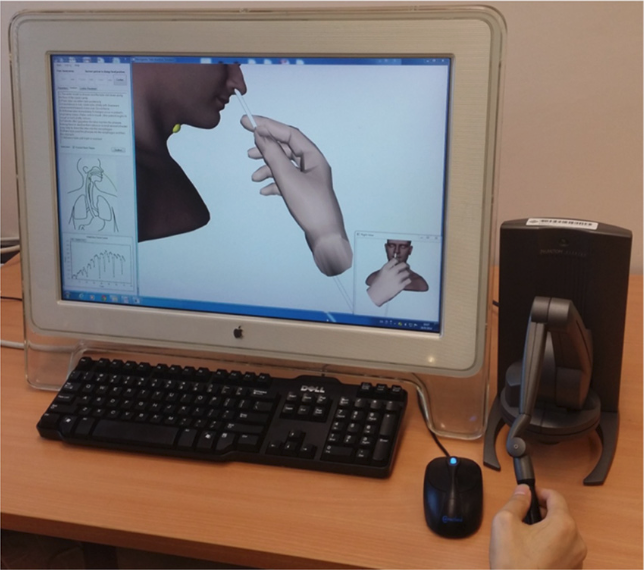
\includegraphics[width=7.5cm]{pictures/haptic_arm.png}
    \caption[Bras haptique simulant l'insertion d'une sonde naso-gastrique \parencite{Choi2015103}]{Exemple de bras haptique servant à simuler l'insertion d'une sonde naso-gastrique, avec un modèle 3D mis à jour en temps réel à côté \parencite{Choi2015103}.}
    \label{fig:haptic_arm}
\end{figure}

Par exemple, dans le cadre de la simulation de l'insertion d'une sonde naso-gastrique, Choi \textit{et al.} ont utilisé un modèle physique 3D de tête humaine conjointement avec un bras haptique \ref{fig:haptic_arm} \parencite{Choi2015103}. Ce système permet de générer la sensation d'une insertion et de buttée si jamais la sonde touche une partie de la gorge, et ainsi de pouvoir ajuster le geste en temps réel.

Dans le domaine industriel, Chamaret \textit{et al.} ont capturé des mouvements à l'aide d'un dispositif appelé « spidar » \parencite{Chamaret2010}. Le but était d'étudier et d'évaluer différentes procédures d'assemblage et de démontage d'un phare de voiture, dans un environnement virtuel. Les modèles 3D, ainsi que le retour de force, étaient adaptés à la morphologie de l'utilisateur. L'objectif était d'évaluer empiriquement la capacité de l'utilisateur à accomplir la tâche demandée, en accord avec le nombre de collisions.\\

Les dispositifs haptiques disposent souvent d'un espace de travail limité (bras à retours d'efforts), contraignant l'utilisateur dans ses mouvements à cet espace (bras à retour d'effort à socle fixe) ou par le poids de ces dispositifs (veste tactile, bras à retours d'efforts portatifs, gants à retour d'efforts).  Cependant, les situations d'apprentissage du geste ne se limitent pas toujours à un espace de travail restreint. Dans le contexte de l'apprentissage de gestes sportifs ou artistiques par exemple, le corps ainsi que les objets manipulés peuvent évoluer dans un espace 3D avec un volume/espace de travail conséquent.

Dans ces cas, plusieurs méthodes de suivi de l'objet existent. L'une d'elles utilise des marqueurs réfléchissants placés sur l'objet à suivre, afin d'en obtenir la trajectoire dans l'espace et le temps, au même titre que les méthodes vues précédemment servant à capter le corps d'un humain. Le positionnement de ces capteurs sur l'objet en question (Fig. \ref{fig:markers}) doit faire l'objet d'une attention particulière, afin de limiter les problèmes d'occlusion. Shapira \textit{et al.} utilisent un ensemble de caméra infrarouges combinées à des casques de réalité virtuelle et des objets (des cubes mous et des jouets divers) équipés de de sphère réfléchissantes, afin d'être captées et utilisées au sein de l'environnement virtuel \parencite{Shapira2016TVR}. Un autre test en utilisant des bâtons réfléchissants à la place des sphères a été réalisé, cependant, les objets étant manipulés par des enfants, ces marqueurs étaient le plus souvent occultés par ces derniers. Ainsi, les sphères réfléchissantes positionnées sur les arrêtes des objets à manipuler se sont révélées plus efficaces pour réussir à suivre les déplacements et rotations des objets dans l'espace.

\begin{figure}
    \centering
    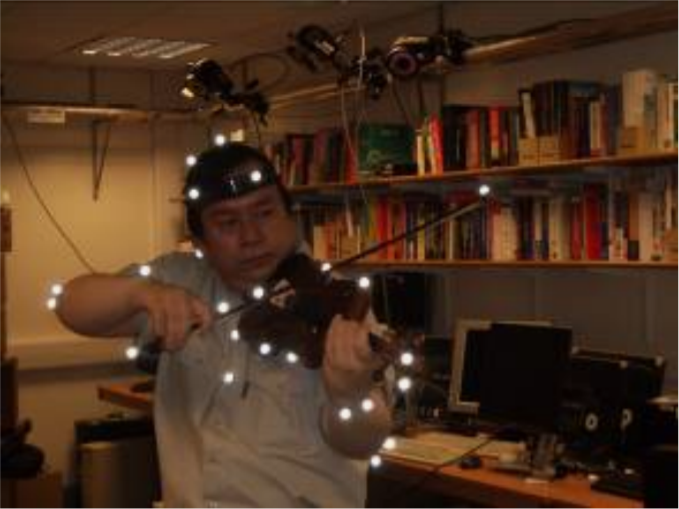
\includegraphics[width=7.5cm]{pictures/markers.png}
    \caption[Marqueurs réfléchissants sur une personne et un objet \parencite{Ng2008}]{Exemple de marqueurs réfléchissants positionnés sur une personne et un objet \parencite{Ng2008}.}
    \label{fig:markers}
\end{figure}

%Dans le cadre de l'apprentissage du violon, des capteurs réfléchissants placés sur l'archet et le corps du violon ont été utilisés dans \parencite{Ng2008}, afin de suivre sa position dans le temps et l'espace. Ces capteurs, d'une taille d'un centimètre de diamètre, étaient captés par 12 caméras infrarouge disposées autour de la personne réalisant le mouvement, afin de minimiser au maximum la perte de tracking d'un des capteurs à cause d'une occlusion. La position des marqueurs sur l'instrument était également susceptible de gêner le mouvement du violoniste. Pour pallier ce problème, un modèle statique de l'instrument ayant tous les marqueurs nécessaire à la captation du violon a été créé, puis un modèle avec moins de marqueurs a été utilisé pour le jeu, le modèle final du violon étant reconstruit en calculant les positions des marqueurs manquants par rapport au modèle statique.\\

\subsection{Bilan sur les dispositifs de captation de mouvement}
La qualité des données produites par les différentes méthodes d'acquisition peut varier grandement, notamment à cause des problèmes spécifiques aux matériels utilisés (problèmes d'occlusion pour les caméras RGB-D, problème de dérive pour les capteurs inertiels portés). Cependant, les matériels de captation fournissant les données plus précises possèdent un coût d'achat parfois prohibitif, ainsi qu'une mise en place plus contraignante. De plus, ils nécessitent parfois l'utilisation d'une chaîne de traitement (intégrée aux logiciels fournis avec système de capture ou non) afin d'obtenir des données exploitables. Concernant les systèmes moins coûteux, tels que la captation à l'aide de caméras \textit{RGB-D} ou de combinaison de capteurs inertiels, la mise en place du matériel est moins contraignante (en terme de temps et d'espace), et nécessite moins de traitements afin d'obtenir des données utilisables. Quelle que soit l'utilisation faite du mouvement, il faut être en mesure de disposer de données non-bruitées par les systèmes de capture. Les systèmes au sein desquels sont utilisées des données de mouvement doivent souvent intégrer une chaine de traitements du mouvement, soit pour le filtrage, soit pour l'extraction d'informations sur une partie précise du mouvement global. Ce besoin est crucial dans les systèmes dédiés à l'apprentissage de mouvements, indépendamment du contexte applicatif.

Dans le contexte de la thèse, la captation par combinaison de capteurs inertiels a été retenue. Plus précisément, il s'agit de la combinaison Perception NEURON. L'installation et la calibration d'une telle combinaison est rapide, et elle n'encombre que marginalement la personne la portant. La possibilité d'utiliser de tels dispositifs sans être contraint à un espace de travail fixe permet de mieux s'adapter au contexte du geste à effectuer (contraintes d'environnement, d'espace nécessaire, \textit{etc.}). Le logiciel fourni, servant à récupérer les informations transmises par la combinaison, intègre une série de pré-traitements, afin de filtrer les données de mouvement obtenues. Les retours proposés par le système se basant sur le mouvement seul, et étant donnés par un expert ou le système lui-même, il n'y a pas besoin d'utiliser un système de retours haptiques. Enfin, le coût faible d'une telle combinaison par rapport aux systèmes de captation plus perfectionnés est des atouts dans le contexte d'un EIAH permettant d'aider à l'apprentissage de geste qui se veut utilisables par tous.

%\section{Nombre de données}
%Dans un contexte informatique, plusieurs stratégies existent pour améliorer l'apprentissage du geste. Ainsi, au même titre que le type des données peut être différent, la quantité utilisée peut l'être également.

%L'utilisation d'un squelette 3D d'expert reproduisant le mouvement est une manière d'apprendre le mouvement analogue aux techniques se passant d'outils informatique.

%L'utilisation de modèles experts mis en parallèle avec celui de l'apprenant est une piste qui a été exploré dans l'apprentissage du geste \parencite{Yoshinaga20151497} \parencite{Kora20151559}. Dans ce cas, le geste de l'expert est enregistré, et est rejoué à côté de celui de l'apprenant, ou en les superposant. Le systèmee proposé par \parencite{Yoshinaga20151497} se base sur plusieurs modèles d'experts, à partir desquels il est possible d'obtenir un expert " moyen " (\textit{i.e.} une moyenne des modèles experts), l'expert médian, ou celui le plus proche de l'apprenant en terme de morphologie.


%La superposition virtuelle du mouvement de l'apprenant et de celui de l'expert est une piste qui a été exploré dans l'apprentissage du geste. Dans le domaine de l'archerie japonaise, Yoshinaga et Soga ont développé un système basé sur une caméra RGB-D (Kinect), afin de capturer le mouvement de l'apprenant \parencite{Yoshinaga20151497}. Dans ce système, des mouvements d'experts ont été préalablement capturés à l'aide d'une caméra RGB-D (Kinect), permettant ainsi à l'apprenant de se comparer avec les modèles experts. Le modèle choisi peut être celui d'un expert en particulier, ou une combinaison (moyenne) des modèles, ou encore le modèle étant le plus proche morphologiquement de l'apprenant. Ce système nécessite donc la capture d'un certain nombre d'experts, pour proposer une large gamme de morphologies. L'analyse est ici empirique, effectuée soit par un expert, soit par l'apprenant lui-même en observant la superposition des deux gestes. Kora \textit{et al.} ont utilisés de nombreux dispositifs (casque de réalité virtuelle avec caméra, Kinect. \textit{etc.}) afin de construire un système d'apprentissage du golf \parencite{Kora20151559}. Grâce à la superposition du squelette de l’apprenant et du squelette de l’expert, l’utilisateur est capable de voir son mouvement en temps réel, et ainsi essaye de coller au mieux au mouvement expert. Cependant, cet affichage en temps-réel peut être perturbant et aucune information pédagogique n’est extraite de ce processus. Yamaoka \textit{et al.} propose un système permettant de capturer le mouvement de l'apprenant et de lui donner un retour sur sa performance, dans le contexte du lancer de disque \parencite{YAMAOKA2013912}. Les données sont capturées à l'aide d'une caméra RGB-D (Kinect), puis le mouvement est segmenté en 3 parties, correspondant à la phase de pré-mouvement, mouvement, et post-mouvement. Ces phases sont extraites automatiquement, en observant la position relativement des articulations entre elles, et en segmentant quand un seuil est dépassé. Le retour sur le mouvement est donné selon 5 aspects: (a) mouvement arrière suffisant (avant le lancer), (b) hauteur de la main droite suffisante, (c) transition de hauteur de la main droite, (d) angle de l'épaule droite adéquat, (e) rotation de la hanche suffisante. Les consignes données à l'apprenant sont de la forme " Levez votre main droite ", ou encore " votre hanche doit plus tourner ". Les résultats ne montrent pas d'amélioration significative du résultat du lancer avec le système de conseils mis en place. Ng s'est intéressé à l'apprentissage du violon \parencite{Ng2008}. La capture du mouvement s'effectue uniquement sur l'instrument et l'archet, à l'aide de capteurs réfléchissants. La position des différents éléments nécessaire au jeu est ensuite affichée grace à l'interface proposée. L'EIAH développé permet la visualisation des partitions selon le standard ISO MPEG Symbolic Music Representation (SMR), l'écoute du morceau, un système de tracking en temps réel du mouvement de l'apprenant, ainsi que l'écoute du jeu, permettant de donner des conseils et de proposer de " tourner la page " des partitions en temps réel. Le système propose également une analyse des mouvements à l'aide de clustering, afin de détecter automatiquement quel style de jeu est utilisé (\textit{e.g.} tenuto, staccato, spicato, \textit{etc.}).

\section{Environnements informatiques pour l'apprentissage de gestes}
Il existe de nombreux EIAH dédiés au geste. La finalité de l'apprentissage des gestes au sein de ces systèmes est variée : apprentissage actif impliquant d'avantage l'étudiant \parencite{Xu2019Ptt}, rééducation \parencite{Alankus2010TCG} \parencite{Baldominos2015AAt}, amélioration de la performance sportive \parencite{Maes2012DtM}, \textit{etc.} Ces catégories ne sont pas exclusives, et les systèmes développés se retrouvent souvent à l'intersection de plusieurs d'entre elles. Les domaines d'application sont également variés : médical (\textit{e.g.} analyse de postures \parencite{Aminian2004Chm}, chirurgie \parencite{BMT_2015}, etc.), sport (\textit{e.g.} danse \parencite{Maes2012DtM}, archerie japonaise \parencite{Yoshinaga2015Doa}, lancer de disque \parencite{Yamaoka2013FoF}), et les techniques utilisées peuvent également faire appel à la réalité virtuelle, par exemple \parencite{Kyan2015ABD}. Pour chaque EIAH, il est possible d'identifier des caractéristiques qui lui sont propres : domaine d'application, objectif visé de l'apprentissage, objectif visé de la ou des tâches à apprendre, prise en compte des besoin d'observation et fonctionnels de l'enseignant, utilisablitié vis-à-vis de l'usager afin de créer et d'évaluer une nouvelle tâche, type de données utilisées pour l'analyse du geste, méthodes d'analyse, retours faits à l'apprenant, \textit{etc.}  En effet, un EIAH sera efficace et démocratisable si l'usager a été placé au cœur de sa conception afin de : (i) répondre à ses besoins d'observation et fonctionnels, (ii) prouver son utilisabilité et (iii), des modèles génériques de conception ont été extraits afin de minimiser la réingénierie en cas de modification de la tâche, des observations et du domaine d'application. Cette section étudie les principaux EIAHs basés « geste » selon ces caractéristiques.

%Le regroupement de ces caractéristiques permet de mettre en évidence un manque d'EIAH dédiés à l'apprentissage du geste réutilisable dans d'autres contextes sans nécessiter de réingénierie conséquente, à cause d'une dépendance trop forte au matériel ou au domaine applicatif retenu.

\subsection{Quelques exemples significatifs d’EIAH pour apprendre des gestes}
Dans le domaine médical, la rééducation nécessite par exemple la répétition de gestes permettant de renforcer une partie du corps, ou de réapprendre à utiliser un membre. Il est possible de faciliter la répétition de certains de ces gestes à l'aide d'interfaces dédiées. Baldominos \textit{et al.} ont développé un EIAH permettant de faire répéter les gestes requis par le médecin pour la rééducation de parties spécifiques du corps \parencite{Baldominos2015AAt}. Dans cette étude, les exercices sont focalisés sur un travail des adducteurs, ainsi que les abducteurs. La mise en situation proposée est celle d'un gardien de but (Fig. \ref{fig:eiah_baldominos}). L'expert peut intervenir ou non dans la séance de rééducation. Si l'expert est présent, il peut choisir le moment du tir du ballon, la vitesse ainsi que de la hauteur de la balle. Dans le cas d'une session d'apprentissage sans expert, le système commence par effectuer des tirs bas, espacés dans le temps, puis augmente ou diminue l'intensité des deux paramètres (hauteur et temps entre les tirs) en fonction du score du patient. Dans les deux cas, une augmentation progressive de la difficulté de la tâche à effectuer permet d'augmenter l'amplitude du mouvement nécessaire, et ainsi de faire progresser le patient. De plus, l'utilisation de dispositifs tels qu'un casque de réalité virtuelle masque les parties du corps, ce qui demande une concentration accrue afin de synchroniser ses mouvements et d'être capable de se situer dans l'espace. %Cette capacité à percevoir les différentes parties de son corps à l'aide des récepteurs sensoriels musculaires et ligamentaires s'appelle la proprioception, et le travail supplémentaire nécessaire au développement de cette perception augmente l'efficacité du traitement, tout en diminuant sa durée \parencite{Missaoui2009Hfd}.

\begin{figure}
    \centering
    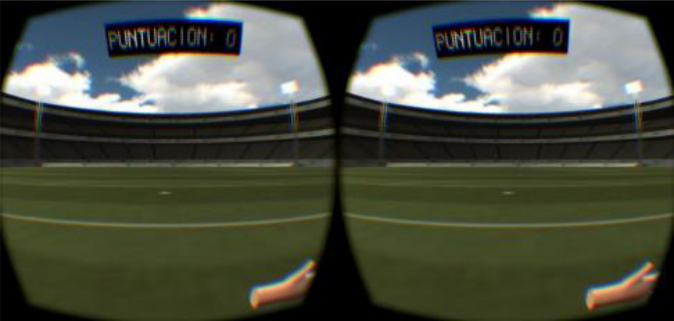
\includegraphics[width=\textwidth]{pictures/eiah_baldominos.png}
    \caption[EIAH pour la rééducation \parencite{Baldominos2015AAt}]{L'environnement de réalité virtuelle proposé par \parencite{Baldominos2015AAt}. La mise en situation dans un cadre crédible par rapport aux exerciecs à effectuer permet d'augmenter l'implication du patient \parencite{Baldominos2015AAt}.}
    \label{fig:eiah_baldominos}
\end{figure}

Les travaux de Alankus \textit{et al.} proposent un système permettant d'engager plus fortement les victimes d'attaque cardiaque lors de la rééducation à domicile \parencite{Alankus2010TCG}. Après une attaque cardiaque, il y a souvent une perte de mobilité de la part du patient. Dans le cadre de la rééducation post-attaque cardiaque, il est souvent nécessaire pour le patient de répéter des gestes, afin de retrouver une certaine mobilité. Ces gestes sont définis par l'expert, en fonction de la gravité des lésions cérébrales et de l'avancée de la rééducation. Bien que les séances avec les spécialistes soient dédiées à ces gestes, la durée, ainsi que la fréquence de ces séances est insuffisante; c'est pourquoi le patient doit également réaliser des gestes répétés chez lui.
%Cependant, seulement un tiers des personnes font suffisamment de répétition de ces mouvements \parencite{Shaughnessy2006TaM}. Ce système offre une motivation supplémentaire à l'aide de la gamification des exercices à réaliser.
Dans ce contexte, les mouvements sont capturés à l'aide de dispositifs communs et abordables : webcam et Wiimote™. Plusieurs jeux ont été développés : déplacement de personnages dans l'espace, jeu de course automobile, lancer et rattrapage de balle de baseball, jardinage (élimination des mauvaises herbes en laissant les fleurs intactes), \textit{etc.} Chacun de ces jeux se concentre sur un mouvement précis à réaliser, allant de mouvement amples (balayage du bras) à des mouvements fins (utilisation de contrôleurs analogiques pour déplacer un personnage). Ils ont été développés en collaboration avec des médecins, afin de solliciter les capacités cognitives du patient, ainsi que les parties du corps concernées par la rééducation. Ils permettent d'activer des parties du cerveau différentes, en stimulant soit la mémoire, le contrôle d'une partie du corps spécifique, la coordination des membres du corps ou les facultés d'anticipation. Le système peut lui-même modifier la difficulté des jeux (et donc l'intensité des exercices), et il est également possible pour l'expert de personnaliser les jeux, afin de les adapter aux différents patients. Par exemple, il peut définir un ensemble de valeurs correspondant à différents niveaux de difficultés, afin que cette difficulté s'adapte au patient pour que l'exercice propose toujours un défi suffisamment élevé afin d'améliorer l'efficacité de la rééducation. Dans le cas du jeu Pong (un des jeux proposés par le système), la taille de raquette et de la balle, ainsi que la vitesse de la balle peuvent être changées.

Lorsque l'objectif est de réussir un geste menant à la manipulation d'un objet,  comme dans le domaine de la chirurgie, le système peut combiner plusieurs types de données hétérogènes, afin d'évaluer plusieurs modalités. Par exemple, le système utilisé par Toussaint  permet de combiner les données de mouvement d'un bras haptique (utilisé pour simuler la manipulation d'un trocard) ainsi que le retour de force associé (simulant les variations de densités du corps humain et des vertèbres), et d'un oculomètre, afin de suivre la trajectoire du regard au cours d'une opération (Fig. \ref{fig:eiah_toussaint}) \parencite{BMT_2015}. Les connaissances mises en jeu sont appelé « perceptivo-gestuelles », car elles combinent la vision et le geste. Un algorithme d'extraction de \textit{patterns}, \textit{PhARules}, inspiré de \textit{CMRules}, permet d'extraire des séquences d'actions en fonction des phases dans lesquelles elles sont réalisées. Les détail du parcours de l'apprenant, ainsi que les interactions pour chaque séquence de l'opération sont fournis. Ces interactions peuvent être de type « contrôle \textit{a priori} » (\textit{e.g.} une observation des signes vitaux du patient avant l'opération), « contrôle \textit{a posteriori} » (\textit{e.g.} une observation des signes vitaux du patient après être intervenu sur le patient) ou « mixte » (\textit{e.g.} prise d'information et manipulation du patient en simultané). Selon le degré de réussite de la procédure, le système propose un retour à l'apprenant : réalisation d'un exercice complémentaire sur un nouveau cas clinique simulé afin de renforcer l'acquisition des connaissances sur un point précis, proposition de révision des cours théoriques, approfondissement de la connaissance du cas clinique qui vient d'être traité.

\begin{figure}
    \centering
    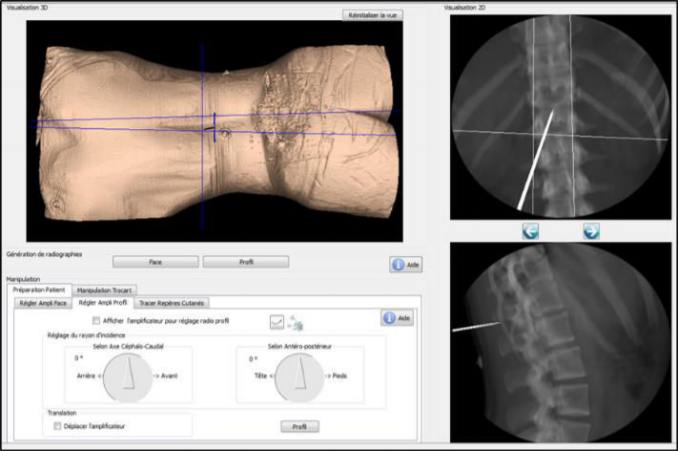
\includegraphics[width=\textwidth]{pictures/eiah_toussaint.png}
    \caption[EIAH pour la chirurgie orthopédique \parencite{BMT_2015}]{Le système utilisé par \parencite{BMT_2015} permet de combiner les données d'un oculomètre ainsi que d'un bras haptique afin de donner un retour couvrant tous les aspects importants d'une procédure chirurgicale orthopédique \parencite{BMT_2015}.}
    \label{fig:eiah_toussaint}
\end{figure}

%Des études telles que Ferrari \textit{et al.} proposent d'intégrer une évaluation des mouvements en contexte industriel par rapport aux normes de sécurité et d'ergonomie \parencite{Ferrari2018MAS}. L'étude se base sur la capture du mouvement, mais également l'analyse de la productivité d'un opérateur d'une part, et d'autre part l'analyse de la posture, de la position et de différentes modalités (telles que la distance effectuée, la vitesse moyenne au cours de l'activité, l'amplitude verticale) pour des articulations précises, en fonction de la tâche à accomplir : mains pour la prise d'objets, haut du corps pour le déplacement du corps, par exemple. Ces travaux se basent sur les méthodes d'évaluation ergonomiques internationales OWAS, REBA, NIOSH et EAWS. Les informations extraites et analysées du mouvement sont le déplacement et la vitesse de certaines parties du corps, les mouvements verticaux dus au soulèvement et la pose d'objets, le chemin suivit de l'opérateur en poste ainsi que la trajectoire de sa main, l'utilisation de l'espace de travail, la fréquence ainsi que la durée des opérations de déplacement d'objet, et la répartition du temps entre les tâches dites à valeur ajoutée (exécution d'une tâche) et les tâches sans valeur ajoutée (marcher, prendre un objet, etc.). Le système est configuré pour un environnement de travail particulier. La connaissance de l'expert est réduite à un ensemble de règles d'ergonomies utilisées. Bien que le système propose une évaluation du mouvement, aucune recommandation supplémentaire n'est fournie par le système quant aux changements à effectuer, tant sur le poste de travail que sur le geste de la personne. Les données fournies par le système doivent être analysées par une personne à même de les mettre en relation avec le poste de travail occupé, afin d'effectuer des changements soit dans le rythme du travail imposé, soit dans la disposition des éléments du poste de travail.

L'apprentissage de la langue des signes est difficile, et nécessite une pratique régulière pour les non-natifs \parencite{Cooper2011Slr}. La captation et l'analyse des gestes de la langue des signes nécessitent de prendre en compte : (i) toutes les parties du corps situées au-dessus du bassin, en tant qu’éléments signifiant du discours et (ii) la précision et la rapidité des mouvements effectués par certaines parties du corps telles que les mains et les doigts \parencite{Gibet2016IEi}. En utilisant des données enregistrées avec un dispositif low-cost (Microsoft Kinect™), le système développé par Gameiro \textit{et al.} permet de faciliter l'apprentissage de la langue des signes grâce à deux modes d'utilisation : le mode « classe », et le mode « compétition » (Fig. \ref{fig:eiah_gameiro}) \parencite{Gameiro2014KST}. Le mode classe met l'apprenant face à une situation d'apprentissage où il doit répéter les signes présents à l'écran, jusqu'à ce que le signe soit correctement fait. Le mode compétition est gamifié, et propose une situation de type quizz télévisé, où le but est de répondre en signant à des questions permettant de tester les connaissances de la personne. L'autre défi du mode compétition consiste en une évaluation des capacités de l'apprenant à épeler et signer correctement un mot, en composant les signes des lettres successives. Dans ce cas, l'évaluation est binaire : soit le geste correspond au signe à réaliser, soit il ne correspond pas. L'évaluation se fait à l'aide d'un masquage des données de l'apprenant par les signes correspondant aux lettres à signer présents dans la base de données. Bien que présentant des résultats positifs avec des classes d'étudiants en langage des signes, les auteurs notent que la reconnaissance automatique des signes de l'apprenant est meilleure lorsque la base de données de signes de référence est construite à partir des mouvements de l'apprenant. Cela s'explique par les différences morphologiques entre les différentes personnes ayant utilisé le système, à cause de l'absence de normalisation ou de mise à l'échelle des données capturées par la caméra.

\begin{figure}
    \centering
    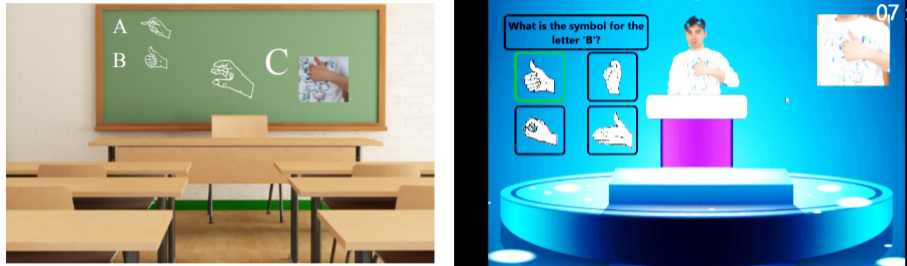
\includegraphics[width=\textwidth]{pictures/eiah_gameiro.png}
    \caption[EIAH pour l'apprentissage de la langue des signes \parencite{Gameiro2014KST}]{Le système proposé par \parencite{Gameiro2014KST} met d'une part l'apprenant dans une situation classique d'apprentissage (à gauche), puis permet de tester les connaissances à l'aide d'une gamification type " quizz télévisé " (à droite) \parencite{Gameiro2014KST}.}
    \label{fig:eiah_gameiro}
\end{figure}

L'EIAH développé par Xu \textit{et al.} permet de faire apprendre à des enfants certains gestes, complexes ou non \parencite{Xu2019Ptt}. Dans cette étude, ces gestes étaient liés à la culture Chinoise : manipuler un métier à tisser, tirer à l'arc, chevaucher un cheval, manipuler des panneaux, \textit{etc.} Les gestes sont acquis à l'aide d'une caméra \textit{RGB-D}. Le mouvement est segmenté dans un premier temps, à l'aide d'un modèle de Markov caché, comparant le mouvement complet de l'apprenant à plusieurs combinaisons de mouvements issus de la base de données de mouvements à effectuer. La combinaison de mouvements ayant la plus grande similitude avec les gestes de l'apprenant est choisie comme modèle du geste réalisé par l'apprenant, et le découpage du mouvement de l'apprenant s'effectue selon cette combinaison. La comparaison du geste de l'apprenant à celui à effectuer intervient à la suite de la segmentation, et est également réalisée par un modèle de Markov caché, à l'aide plusieurs modules permettant chacun de reconnaître un geste. Ainsi, en décomposant le mouvement en plusieurs parties, il est possible de comparer chaque étape d'un geste continu aux gestes cible présents dans la base de données de gestes, et donc de déterminer si le geste est réussi ou non. S'il ne l'est pas, le système va proposer un exercice permettant de se focaliser sur la ou les parties du geste ratées, à l'aide d'un autre modèle de Markov caché (Fig. \ref{fig:eiah_xu}). Ce réseau se base sur les résultats de l'analyse des gestes du précédent : ainsi, en chaque point où le geste de l'apprenant n'est pas conforme au geste attendu, le système va être en mesure de proposer plusieurs ressources différentes (explications textuelles, vidéo de démonstration, \textit{etc.}) pour expliquer ou montrer à l'apprenant quel est le geste attendu. Par exemple, dans le cas de la manipulation du métier à tisser, le système peut détecter si l'apprenant ne regarde pas le métier à tisser pendant la tâche, ou si la distance entre son corps et le métier à tisser est trop grande, et lui faire visualiser une vidéo lui montrant la posture à adopter pour réaliser cette tâche. L'apprentissage du geste est ainsi amélioré en faisant répéter des parties spécifiques à l'apprenant, avant de passer à la suite du parcours. De cette manière, il est possible de mettre l'accent sur les mouvements que l'apprenant a du mal à réaliser.

\begin{figure}
    \centering
    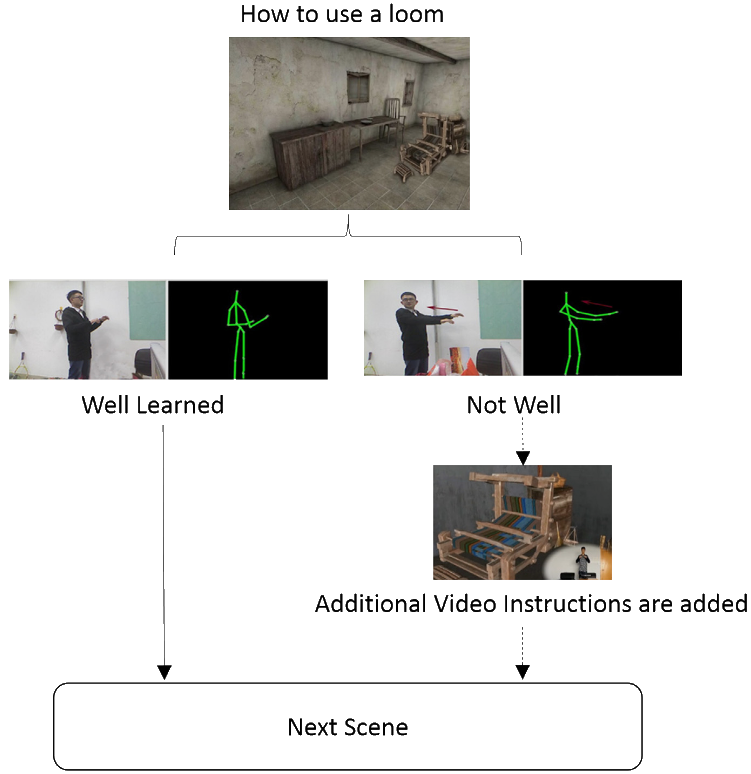
\includegraphics[width=7.5cm]{pictures/eiah_xu.png}
    \caption[EIAH permettant de corriger des parties spécifiques du geste \parencite{Xu2019Ptt}]{L'adaptation du parcours d'apprentissage proposé par Xu \textit{et al.} permet de corriger des parties spécifiques du mouvement de l'apprenant \parencite{Xu2019Ptt}.}
    \label{fig:eiah_xu}
\end{figure}

Le domaine artistique et sportif fait usage des EIAH pour l'apprentissage de gestes. Chan \textit{et al.} ont développé un système permettant d'apprendre des mouvements de danse, en se basant sur des données de mouvement d'expert enregistrées au préalable à l'aide d'un système basé sur une combinaison de capteurs réfléchissants et des caméras infrarouge, afin de l'afficher sur un écran \parencite{Chan2011}. En observant les gestes de l'expert, l'apprenant le reproduit ensuite, et ses données sont capturées, afin d'être comparées à celles de l'expert. Les données sont stockées sous forme de squelettes 3D, à partir desquels plusieurs analyses sont faites. Dans ce système, les différences morphologiques entre l'apprenant et l'expert sont atténuées à l'aide d'une normalisation des positions des articulations par la somme des membres du corps. Plusieurs retours sont offerts à l'apprenant. En premier lieu, une visualisation en temps réel du mouvement de l'expert et de celui de l'apprenant est proposée, en colorant les différentes parties du corps de l'apprenant en fonction des différences avec le geste de l'expert (lorsqu'un certain seuil de distance est franchi entre les positions des articulations de l'expert et de l'apprenant). Il est également possible de rejouer le mouvement au ralenti, afin de mieux voir les différences entre les gestes. Enfin, un score de performance global, correspondant à la somme des distances des articulations de l'apprenant par rapport à celles de l'expert, est fourni à l'apprenant.

Le système d'aide à l'apprentissage de la danse développé par Maes \textit{et al.} propose une approche différente pour la visualisation des mouvements de l'expert \parencite{Maes2012DtM}. Trois étapes sont proposées : la visualisation du mouvement réalisé par l'expert, l'apprentissage en réalisant le geste de manière décomposée afin d'apprendre chaque étape, et l'évaluation à l'aide d'un score indiquant la performance de l'apprenant. La décomposition du mouvement est réalisée de manière automatique, en analysant d'une part le rythme et le tempo de la musique, et d'autre part le mouvement de l'expert réalisant le geste. Les points d'inflexions dans ces valeurs synchronisées avec les tempos sont utilisés comme séparateurs du mouvement. L'expert peut ensuite valider cette séparation avant d'intégrer le geste au système. Le score se base sur le coefficient de corrélation croisée de Pearson entre les données de mouvement de l'expert et celles de l'apprenant, un score de 1 indiquant une similitude parfaite entre les deux gestes, alors qu'un score de 0 indique une dissimilitude complète. L'utilisation de systèmes intégrant un tuteur intelligent (souvent appelés « coachs ») permet de s'affranchir de la présence d'un expert, et donc de l'obligation de se rendre dans un endroit spécifique pour pratiquer, et permet également d'entraîner des personnes en parallèle. Dans ces systèmes, l'expert n'intervient que dans l'enregistrement et l'intégration des données au système, le retour à l'apprenant est fait par le système à l'aide d'un score ou de conseils par exemple.

Dans le domaine du sport, il est également possible de développer de tels systèmes pour la découverte automatique de la différence entre le geste d'un expert et d'un débutant, comme le système proposé par Makio \textit{et al.}, servant à séparer les gestes de service au tennis des professionnels de ceux des amateurs \parencite{Makio2007DoS}. Dans ce cas, le système permet d'extraire dans un premier temps des règles d'associations entre les différentes parties du corps, afin de découvrir les mouvements effectués par l'expert. Dans un premier temps, le mouvement est segmenté à partir des points où la vitesse (sur un des trois axe) d'une articulation spécifiée est égale à zéro. Les parties du mouvement ainsi segmentées sont ensuite comparées entre elles à l'aide du Dynamic Time Warping (DTW), afin d'obtenir un score de similitude. Les mouvements sont ensuite regroupés à l'aide d'un algorithme de clustering, afin de réunir au sein d'un même groupe plusieurs sous-parties du mouvement correspondant au même geste. L'utilisation de deux fenêtres glissantes, l'une active (correspondant aux mouvements ayant une influence sur d'autres mouvements) et l'autre passive (correspondant aux mouvements étant influencés par d'autres mouvements) permet ensuite de détecter les dépendances récurrentes entre les parties du corps lors de la réalisation d'un geste, correspondant aux règles d'association. Une règle ainsi obtenue peut s'écrire

\[ if
  \begin{pmatrix}
  \text{\textit{left ankle 166}} \\
  \text{\textit{right wrist 48}}
 \end{pmatrix}
 then (\text{\textit{left ankle 167}})\]

ce qui correspond à « Si le centre de gravité se situe sur le pied gauche alors que la main droite se déplace vers le bas, alors le pied gauche se déplacera vers le haut » . Dans un deuxième temps, des motifs fréquents de déplacement sont extraits au sein des mouvements, afin d'obtenir une décomposition de ce mouvement. Cette extraction se base sur une réduction de la dimensionnalité des données 3D dans un espace 1D à l'aide d'une analyse en composantes principales (PCA), afin de réduire les temps de calcul. Les séquences sont ensuite réduites à un ensemble symbolique à l'aide du principe de longueur de description minimale \parencite{Rissanen1998SCi}, puis comparées entre elles à l'aide d'une distance euclidienne. Ici, la connaissance experte est directement intégrée au système lors de sa création : dans le cas présent, il s'agit de la trajectoire des poignets dans le contexte d'un service au tennis. Ces données peuvent ensuite être utilisées afin de comparer les données de l'apprenant à celles de l'expert. Ce système permet d'obtenir une visualisation graphique de la trajectoire de la raquette, et permet de mettre en évidence les différences de trajectoires entre les débutants et les experts.\\

Les travaux de Morel sur l'évaluation de gestes sportifs à l'aide de séries temporelles ont conduit à la création d'un EIAH permettant d'apprendre un geste \parencite{Morel2017Mts}. Ce système est développé de manière à être indépendant du sport choisi. Le geste à atteindre est modélisé par le squelette de l'expert effectuant ce geste, et les données sont capturées à l'aide d'un système de marqueurs réfléchissants et caméras infrarouges. Les squelettes de l'apprenant et de l'expert sont recalés spatialement (à l'aide d'une transformation linéaire) et temporellement (à l'aide de l'algorithme du \textit{Subsequence DTW}). Les erreurs spatiales et temporelles sont calculées, à l'aide d'un respectivement, permettant ainsi de donner des indications simples par rapport au geste : « trop haut », « trop bas », « trop à gauche », « trop à droite », « trop en avant » , « trop en arrière » pour les variations spatiales, et « en retard » ou « en avance » pour les variations temporelles. La plus grande erreur de l'apprenant est affichée sous la forme d'une animation de son mouvement, superposé à celui de l'expert, avec la partie du corps en faute colorée en rouge (Fig. \ref{fig:Morel_eiah}). Le processus d'intégration de la connaissance experte au système n'est pas précisé dans l'étude, mais aucune interface de sélection de caractéristiques à observer n'est montée, ce qui suggère que cette intégration se fait au moment de la conception du système, limitant ainsi la facilité de réutilisation du système dans d'autres contextes.

\begin{figure}[h]
    \centering
    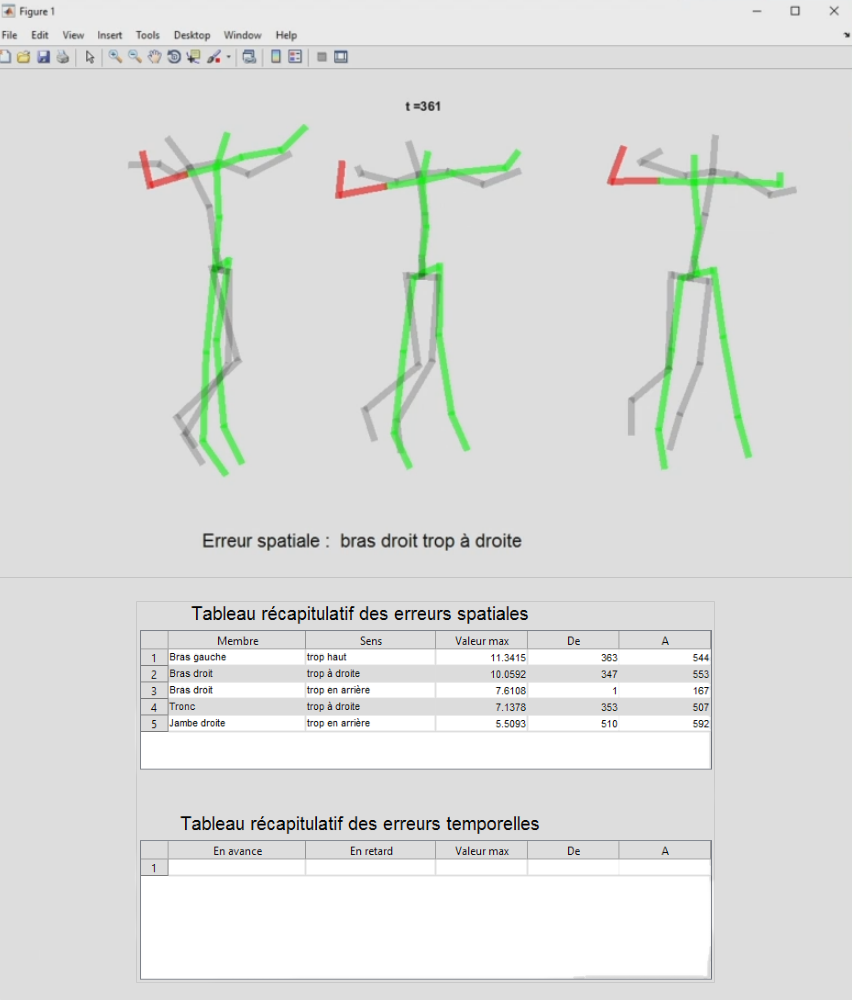
\includegraphics[width=10cm]{pictures/Morel_eiah.png}
    \caption[EIAH pour l'évaluation de gestes sportifs \parencite{Morel2017Mts}]{Le système développé par Morel permet d'afficher les plus grandes erreurs spatiales et temporelles du mouvement de l'apprenant, par rapport à celui de l'expert \parencite{Morel2017Mts}.}
    \label{fig:Morel_eiah}
\end{figure}

Enfin, le système proposé par Le Naour \textit{et al.} a pour but de fournir une aide à l'apprentissage de mouvement en proposant une superposition du modèle de l'apprenant à celui de l'expert, dans un environnement virtuel \parencite{LeNaour2019S3V} (Fig. \ref{fig:LeNaour_eiah}). Les mouvements sont capturés à l'aide d'un système de marqueurs réfléchissants et caméras infrarouges. L'expérimentation présentée dans ces travaux porte sur le lancer au football américain. En premier lieu, une démonstration est effectuée par un expert, et des conseils sont donnés par ce dernier sur les caractéristiques propres à un bon geste (\textit{e.g.} position et rotation des articulations impliquées dans le mouvement, prise de la balle, \textit{etc.}). Après dix lancers d'entraînement, les participants devaient effectuer cinquante lancers, tout en suivant le plus possible le mouvement de l'expert. Plusieurs groupes ont été formés : un groupe sans aucun retour sur la performance, un groupe où le mouvement de l'expert était montré après chaque lancer, un autre où le mouvement de l'expert était montré au participant pendant leur mouvement, suivit de la visualisation de la superposition du mouvement du participant à celui de l'expert, un autre groupe où le mouvement de l'expert était superposé à celui du participant pendant le geste et où le geste de l'expert était visualisé après le lancer, et un dernier où le modèle expert superposé à celui de l'apprenant était visualisé pendant et après le geste. Ont été relevés l'écart-type du calcul de la DTW entre le mouvement de l'apprenant et de l'expert, et la distance par rapport au centre de la cible (le résultat du mouvement). Les résultats montrent que les groupes ayant reçu les retours sous forme de superposition des modèles expert et apprenant ont montrés une amélioration de leur geste. Il est intéressant de noter que l'amélioration du geste n'améliore pas systématiquement la distance par rapport au centre de la cible, et inversement. Ainsi, lors de l'analyse du résultat d'une telle expérimentation, il faut être en mesure de positionner l'objectif final de l'apprentissage : amélioration du geste ou du résultat du geste.

\begin{figure}[h]
    \centering
    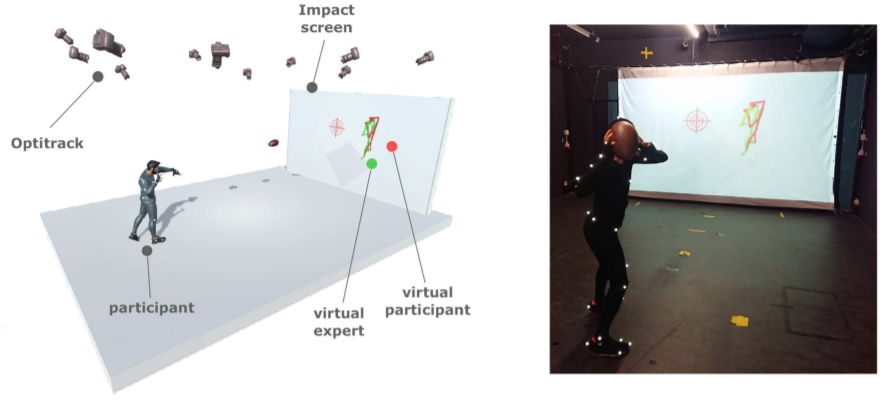
\includegraphics[width=10cm]{pictures/LeNaour_eiah.png}
    \caption[EVAH superposant les gestes de l'apprenant à ceux de l'expert \parencite{LeNaour2019S3V}]{Le système développé par LeNaour \textit{et al.} propose une superposition en temps réel des mouvements de l'apprenant et de l'expert dans un environnement virtuel \parencite{LeNaour2019S3V}.}
    \label{fig:LeNaour_eiah}
\end{figure}

% Probably: Tai-chi sci-hub.tw/10.1109/VR.2017.7892299 \parencite{He2017Iac}

\subsection{Tableau de synthèse}
Tous ces systèmes ont pour point commun d'aider à l'apprentissage de geste, que ce soit en proposant une aide à la décision à l'enseignant, en intégrant les connaissances expertes à un système permettant de s'affranchir de la présence de l'expert, en proposant une évaluation du geste en fonction de critères pré-définis, ou en analysant automatiquement les différences entre les gestes, avec un \textit{a priori} ou non.

Les systèmes où la connaissance experte est intégrée dès la conception permettent de focaliser la conception de l'EIAH sur un problème précis, et ainsi de l'adapter du mieux possible au geste cible (données relevées et utilisées, environnement d'apprentissage du geste, retours à faire à l'apprenant, etc.) \parencite{Baldominos2015AAt, Alankus2010TCG, Gameiro2014KST, BMT_2015, LeNaour2019S3V}. Dans ces cas, il est possible de faciliter l'apprentissage du geste, mais également de proposer des évaluations sous forme de score pertinent dans le contexte applicatif choisi ou de retours donnés par l'expert après visualisation des indicateurs de la performance. Cependant, comme le montre le tableau \ref{tab:eiah_tab}, ces systèmes ne sont pas réutilisables dans d'autres contexte sans nécessiter un processus de réingénierie conséquent : il faut ainsi re-formaliser et réintégrer une autre connaissance experte dans une nouvelle phase de conception, possiblement ré-adapter le système au nouvel environnement dans lequel le geste est réalisé, acquérir de nouvelles données puis les intégrer au processus de traitement, et enfin ré-adapter les retours donnés en fonction des objectifs d'apprentissage.

L'utilisation d'algorithmes d'apprentissage automatique est une méthode qui permet de séparer les gestes de l'apprenant de ceux de l'expert de manière automatique selon des caractéristiques prédéfinies \parencite{Ng2008}. En outre, elle permet également d'observer dans quelle mesure les caractéristiques déterminées au préalable du geste observé varient entre ces mouvements \parencite{BMT_2015}. Ces méthodes nécessitent de disposer d'une base de données d'apprentissage conséquente (\textit{i.e.} de l'ordre du millier de données de mouvement) afin d'être capable de construire une bonne fonction de séparation. En pratique, il est fastidieux de devoir constituer un corpus de données annotées spécifique à un type de mouvement, bien que des bases de données existent (e.g. \textit{Graphics Lab Motion Capture Database} \parencite{CMUDatabase}, \textit{Motion Capture Database HDM05} \parencite{HDM05Database}, \textit{etc.}). Cependant, ces bases sont rarement spécialisées sur une tâche précise, et des variations et spécificités peuvent exister sur le geste à apprendre pour une même tâche et un même enseignant. De plus, l'utilisation d'algorithmes d'apprentissage supervisé suppose d'avoir la connaissance des différentes classes en sortie de l'algorithme, ce qui limite les types de restitution par rapport aux connaissances d'un expert humain, comme montré dans le tableau \ref{tab:eiah_tab}. Bien que l'expert soit en mesure de proposer des caractéristiques, il est possible que les variations de ces caractéristiques puissent mener à la formation de groupes possédant une sémantique plus fine que « réussi / raté » par exemple, permettant de proposer une séparation prenant en compte plusieurs niveaux de réussite du geste, ou menant à la découverte de caractéristiques spécifiques à un type de difficulté ou d'apprenant.

Les systèmes où la découverte des différences significatives entre des groupes de gestes se fait de manière totalement automatique s'affranchissent de l'intégration de la connaissance experte à l'aide du vocabulaire métier, où l'intègrent sous la forme de descripteurs cinématiques, géométriques ou biomécaniques  \parencite{Makio2007DoS} \parencite{Pirsiavash2014AQA}. De nouveaux critères de séparation des gestes acceptables ou non peuvent être découverts. Ils manquent cependant de sémantique dans leur retour : ainsi, il n'est pas possible d'identifier par exemple des groupes ou ensembles de gestes acceptables et non acceptables typiques afin d'étudier les caractéristiques des meilleures stratégies et des erreurs les plus fréquentes. De plus, il peut être difficile de fournir des retours pertinents à des personnes ne possédant pas des compétences poussées en physique, mécanique, \textit{etc.}, car l'interprétation de données cinématiques, géométriques, \textit{etc.} exige d'avoir ces connaissances. Ainsi, les conseils apportés par un tel système doivent non seulement être pertinent dans le contexte applicatif retenu, mais également compréhensibles et utilisables par des personnes sans connaissances scientifiques avancées, ce qui n'est pas toujours réalisable.


\pagebreak
\begin{landscape}
\begin{table}[]
\resizebox{\linewidth}{!}{\begin{tabular}{|l|l|l|l|l|l|l|l|l|l|}
\hline
\multicolumn{1}{|c|}{Auteurs} & \multicolumn{1}{c|}{Domaine} & \multicolumn{1}{c|}{Objectif visé} & \multicolumn{1}{c|}{\makecell[l]{Acquisition\\des données}} & Modélisation des connaissances & \multicolumn{1}{c|}{Analyse} & \multicolumn{1}{c|}{Acteur de la restitution} & \multicolumn{1}{c|}{Information restituée} & \multicolumn{1}{c|}{\makecell[l]{Visualisation du geste\\ou de la restitution}} & \multicolumn{1}{c|}{Généricité} \\ \hline

Yoshinaga et Soga & \makecell[l]{Sport\\Archerie Japonaise} & \makecell[l]{Amélioration du geste\\par rapport aux\\modèles experts} & \makecell[l]{Caméra RGB-D\\(Kinect)} & \makecell[l]{Corpus de squelettes 3D\\ d'experts (enregistrement ad-hoc)} & \makecell[l]{Empirique : analyse visuelle de \\l'expert du squelette 3D de\\l'apprenant effectuant le\\mouvement} & Expert & \makecell[l]{Différences de positions entre les\\mouvements de l'expert et l'apprenant} & \makecell[l]{Superposition de l'apprenant\\et des modèles de coachs} & \makecell[l]{Générique, nécessite de réintégrer\\des modèles experts dans le système} \\ \hline

Kora et al. & \makecell[l]{Sport\\Golf} & Amélioration du swing & \makecell[l]{Caméra RGB-D,\\caméra sur casque\\de réalité virtuelle} & Un modèle d'expert (squelette 3D) & \makecell[l]{Empirique (par l'étudiant) :\\ visualisation des différences\\ entre le modèle expert et son geste} & Aucune restitution & Aucune information restituée & \makecell[l]{Superposition de l'apprenant\\et du modèle expert\\en temps réel} & \makecell[l]{Dépendance totale du système\\au matériel et au domaine applicatif} \\ \hline

Yamaoka et al. & \makecell[l]{Sport\\Lancer de disque} & \makecell[l]{Position des articulations\\lors du lancer} & \makecell[l]{Caméra RGB-D\\(Kinect)} & \makecell[l]{Positon relative des articulations\\entre elles dans les différentes étapes\\du mouvement (défini par un expert)} & \makecell[l]{Automatique : comparaison de\\valeurs à des seuils} & système (textuel) & Positions des membres à corriger & \makecell[l]{Retours générés automatiquement\\à partir de l'analyse} & \makecell[l]{Nécessite de re-formaliser la connaissance experte\\au sein du système (re-conception)} \\ \hline

Ng & \makecell[l]{Musique\\Violon} & \makecell[l]{Détermination du\\style de jeu} & \makecell[l]{Capteurs\\réfléchissants\\(sur l'archet\\et le violon)} & \makecell[l]{Représentation symbolique du son\\(système SMR), descripteurs du\\mouvement (amplitude, vitesse, durée)} & \makecell[l]{Automatique (clustering sur les\\descripteurs extraits)} & \makecell[l]{Enseignant et système\\(visualisation de la\\similitude des\\mouvements entre\\eux)} & \makecell[l]{Mode de jeu, durée, position de l'archet\\ et de l'instrument, vitesse de jeu,\\amplitude du mouvement} & \makecell[l]{Visualisation 3D du mouvement du\\violon et de l'archet, regroupement\\ des mouvements en fonction de\\leurs caractéristiques communes} & \makecell[l]{Dépendance totale du système au matériel\\et au domaine applicatif} \\ \hline

Choi et al. & \makecell[l]{Médical\\Insertion de\\sonde nasogastrique} & \makecell[l]{Apprentissage de la\\procédure d'insertion} & Bras haptique & \makecell[l]{Modèle 3D  de patient vérifiant les\\collisions frictions, etc.\\Procédure complète et étapes clés\\modélisées sous la forme\\d'un arbre de décision} & \makecell[l]{Empirique par l'expert (à partir\\de métriques : durée, min et max\\ de force appliquées, nombre d'insertion\\et nombre de deformations du tube)} & \makecell[l]{Expert (retours\\empiriques) et\\le système\\(retours visuels et haptiques)} & \makecell[l]{Visualisation de la position de la sonde\\dans le modèle 3D, retour de force de\\l'instrument, durée, min et max de\\force appliquées, nombre d'insertion et\\nombre de déformations du tube} & \makecell[l]{Visualisation 3D en temps réel de\\la position de la sonde dans un\\modèle 3D d'humain} & \makecell[l]{Dépendance totale du système au matériel et\\au domaine applicatif} \\ \hline

Baldominos et al. & \makecell[l]{Médical\\Réadaptation\\physique} & Rééducation des patients & \makecell[l]{Caméra RGB-D\\(Intellisense)\\et casque de\\réalité virtuelle\\(Oculus Rift)} & \makecell[l]{Position du patient comparée à des\\références fournies par les médecins\\pour les parties du corps concernées} & Empirique : par l'expert médical & Expert médical & Rééducation suffisante ou non & \makecell[l]{Environnement de réalité virtuelle\\dans lequel le patient\\effectue les gestes désirés} & \makecell[l]{Nécessite de re-formaliser la connaissance experte\\au sein du système (re-conception), re-développemen\\de scène virtuelle, dépendance du système\\au matériel utilisé} \\ \hline

Toussaint et al. & \makecell[l]{Médical\\Chirurgie\\orthopédique\\percutanée} & \makecell[l]{Apprentissage de la\\manipulation de l'objet\\pendant la procédure} & \makecell[l]{Bras haptique\\et occulomètre} & \makecell[l]{Séquences d'actions à effectuer par\\ l'apprenant au cours de l'opération} & \makecell[l]{Automatique : analyse de l'ordre des\\séquences d'action} & Système & \makecell[l]{Propose de revoir une partie du cours,\\consulter un cas clinique ou résoudre\\un autre problème sur le simulateur} & \makecell[l]{Visualisation en temps réel de la\\ manipulation de l'objet} & \makecell[l]{Nécessite de re-formaliser la connaissance experte\\au sein du système, dépendance du système\\au matériel utilisé} \\ \hline

He et al. & \makecell[l]{Sport\\Chinese Taichi} & Apprentissage du Taichi & \makecell[l]{Caméra RGB-D\\(Kinect)} & Squelette 3D de référence pour le geste & \makecell[l]{Automatique : comparaison avec modèle\\expert au niveau de la position\\spatio-temporelle selon 3 métriques} & Système & \makecell[l]{Score prenant en compte les 3\\métriques calculées sur le mouvement\\de l'apprenant par rapport au\\mouvement de l'expert} & \makecell[l]{Environnement de réalité virtuelle\\et CAVE} & \makecell[l]{Nécessite de re-formaliser la connaissance experte\\au sein du système (re-conception)} \\ \hline

Chan et al. & Danse & Apprentissage de la danse & \makecell[l]{Caméra infrarouge\\+ marqueurs} & \makecell[l]{Un modèle d'expert (avatar reproduit\\à l'aide du squelette 3D)} & \makecell[l]{Automatique : comparaison de la position\\ des articulations entre l'apprenant et le\\modèle expert} & Système & \makecell[l]{Visualisation du mouvement de\\ l'apprenant et de celui de l'expert,\\coloration des parties du corps non\\synchronisées avec celles de l'expert} & \makecell[l]{Environnement 3D (OpenGL)\\montrant le squelette de\\l'apprenant et le modèle de\\l'expert en train de réaliser\\ les mouvements de danse} & \makecell[l]{Générique par rapport au domaine applicatif,\\nécessite de réintégrer des modèles experts\\dans le système} \\ \hline

Morel (thèse) & Sport & Amélioration du geste sportif & \makecell[l]{Caméra infrarouge\\+ marqueurs} & Un modèle d'expert (squelette 3D) & \makecell[l]{Automatique : décalage spatial et temporel\\à l'aide de la SDTW} & Système & \makecell[l]{Visuelle et textuelle (affichage des 5\\erreurs les plus significatives,\\ainsi que le temps auquel elles\\apparaissent)} & \makecell[l]{Superposition du mouvement\\de l'apprenant par-dessus\\celui de l'expert, mise en évidence\\des erreurs les plus\\ significatives} & \makecell[l]{Nécessite de re-formaliser la connaissance experte\\au sein du système (re-conception)} \\ \hline

Gaimero et al. & Langue des signes & \makecell[l]{Amélioration du signage\\de l'apprenant} & \makecell[l]{Caméra RGB-D\\(Kinect)} & \makecell[l]{Images des signes fait par un ou\\des expert(s)} & \makecell[l]{Automatique : masquage des données de\\l'apprenant par rapport au bon signe\\présent dans la base de données} & Système & \makecell[l]{Réussite ou non du geste\\(restitution binaire)} & \makecell[l]{Affichage de l'image du geste\\capturé} & \makecell[l]{Nécessite de re-formaliser la connaissance experte\\au sein du système (re-conception)} \\ \hline

Xu et al. & \makecell[l]{Apprentissage\\de gestes\\(pas de contexte\\particulier)} & \makecell[l]{Apprentissage de\\gestes spécifiques} & Caméra RGB-D & Corpus de mouvements unitaires & Automatique : modèle de Markov caché & Système & \makecell[l]{Proposition d'exercices adaptés\\au renforcement de l'apprentissage\\des gestes non-maitrisés} & \makecell[l]{Sur le système, par une\\visualisation du geste correct à\\effectuer et des erreurs} & \makecell[l]{Générique par rapport au domaine applicatif, nécessite\\ de réintégrer des modèles experts dans le système} \\ \hline

Maes et al. & Danse & Apprentissage de la danse & \makecell[l]{Caméra infrarouge\\+ marqueurs} & \makecell[l]{Descripteurs du mouvement\\(déplacement du centre du corps\\par rapport au tempo, rotation du corps\\autour de l'axe vertical)} & \makecell[l]{Automatique : calcul de corrélation\\entre les descripteur du mouvement\\de l'apprenant et de l'expert} & Système & \makecell[l]{Score final, correspondant à la\\similitude entre le geste de l'apprenant\\et celui de l'expert} & Affichage du score & Dépendance totale du système au domaine applicatif \\ \hline

Makio et al. & Sport - générique & \makecell[l]{Séparation des gestes\\expert / apprenant} & Non précisé & Descripteurs du mouvement & Automatique & Système & \makecell[l]{Différence au niveau des\\descripteurs du mouvement calculés} & \makecell[l]{Affichage graphique de la\\différence entre les données\\de l'apprenant et de l'expert} & \makecell[l]{Générique par rapport au domaine applicatif, nécessite\\de réintégrer des modèles experts dans le système} \\ \hline

Le Naour et al. & \makecell[l]{Sport\\lancer au football\\américain} & Amélioration du geste sportif & \makecell[l]{Caméra infrarouge\\+ marqueurs} & \makecell[l]{Descripteurs du mouvement\\et résultat du lancer} & Automatique & Système & \makecell[l]{Différence visuelle entre le mouvement\\de l'apprenant et de l'expert} & \makecell[l]{Visualisation du mouvement\\de l'apprenant superposé\\ou non à celui de l'expert\\(en fonction du groupe)} & \makecell[l]{Nécessite de re-formaliser la connaissance experte\\au sein du système (re-conception)} \\ \hline

\end{tabular}}
\caption{Tableau résumant les principales caractéristiques des EIAH vu dans le chapitre.}
\label{tab:eiah_tab}
\end{table}
\end{landscape}
\pagebreak

%\begin{landscape}
%\begin{table}[]
%\resizebox{\linewidth}{!}{\begin{tabular}{m{2cm}m{2cm}m{2cm}m{3cm}m{3cm}m{2cm}m{7cm}m{7cm}m{7cm}}
%
%Nom (Auteur ?) & Objectif & Domaine & Type de données & Matériel de capture                                                          & Données nécessaire & Visualisation & Analyse & {Retours à l'apprenant}                                                                                                    \\ \toprule
%\parencite{Yoshinaga2015Doa} & Archerie japonaise & Sport & Squelette 3D & Caméra RGB-D (Kinect) & Plusieurs captures d'experts & Superposition de l'apprenant modèles de coachs & Empirique & Par un expert \\\arrayrulecolor{gray}\hline
%\parencite{Kora20151559} & Golf & Sport & Squelette 3D & Caméra RGB-D, caméra sur casque de réalité virtuelle & Un expert & Superposition de l'apprenant et du modèle expert en temps réel & Aucune & Aucun \\\arrayrulecolor{gray}\hline
%\parencite{Yamaoka2013FoF} & Lancer de disque & Sport & Squelette 3D & Caméra RGB-D (Kinect) &  &  & Automatique (positon relative des articulations entre elles dans les différentes étapes du mouvement) & Retours générés automatiquement à partir de l'analyse \\\arrayrulecolor{gray}\hline
%\parencite{Ng2008} & Violon & Musique & Données 3D des positions du violon et de l'archet & Capteurs réfléchissants (sur l'archet et le violon) & Une ou plusieurs & Visualisation 3D du mouvement du violon et de l'archet & Analyse du son, détection automatique du style de jeu à l'aide de clustering &  \\\arrayrulecolor{gray}\hline
%\parencite{Choi2015103} & Insertion de sonde nasogastrique & Médical & Position de l'objet (sonde nasogastrique) & Bras haptique & Une & Visualisation 3D en temps réel de la position de la sonde dans un modèle 3D d'humain & Aucune & Retour de force si la sonde bute contre une paroi du modèle 3D \\\arrayrulecolor{gray}\hline
%\parencite{Baldominos2015AAt} & Réadaptation physique & Médical & Squelette 3D & Caméra RGB-D (Intellisense) et casque de réalité virtuelle (Oculus Rift DK2) & Une & Environnement de réalité virtuelle dans lequel le patient effectue les gestes désirés & Analyse par l'expert médical & Retours empiriques par l'expert médical \\\arrayrulecolor{gray}\hline
%\parencite{BMT_2015} & Chirurgie orthopédique percutanée & Médical & Position de l'objet (trocard) & Bras haptique & Une & EIAH proposant une visualisation en temps réel de la manipulation de l'objet & Automatique (par le système) & Propose de revoir une partie du cours, consulter un cas clinique ou résoudre un autre problème sur le simulateur \\\arrayrulecolor{gray}\hline\
%\parencite{He2017Iac} & Chinese Taichi & Sport & Squelette 3D & Caméra RGB-D (Kinect) & Plusieurs captures d'experts & Environnement de réalité virtuelle et CAVE & Automatique (comparaison avec modèle expert au niveau de la position spatio-temporelle selon 3 métriques) & Score prenant en compte les 3 métriques calculées sur le mouvement de l'apprenant par rapport au mouvement de l'expert \\\arrayrulecolor{gray}\hline
%\parencite{Chan2011} & Danse & Danse & Squelette 3D & Caméra infrarouge + marqueurs & Au moins un expert & Environnement 3D (OpenGL) montrant le squelette de l'apprenant et le modèle de l'expert en train de réaliser les mouvements de danse & Automatique : comparaison de la position des articulations entre l'apprenant et le modèle exper) & Visualisation du mouvement de l'apprenant et de celui de l'expert, coloration des parties du corps non synchronisées avec celles de l'expert\\\arrayrulecolor{gray}\hline
%\parencite{Maes2012DtM} & Danse & Danse & Squelette 3D & Caméras infrarouge & Un modèle expert & Environnement 3D montrant le geste à reproduire, les gestes à réaliser et la superposition de l'apprenant et de l'expert & Automatique : score calculé par le système et empirique : évaluation de l'enregistrement vidéo de la danse par un expert & Score de performance globale donné par le système et (facultatif) évaluation qualitative de l'expert\\
%\bottomrule
%\end{tabular}}
%\caption{Regroupement d'EIAH utilisant différentes modalités pour l'apprentissage du geste.}
%\label{EIAH_table}
%\end{table}
%\end{landscape}

\section{Discussion}
L'apprentissage du geste peut prendre place dans de nombreux contextes. Dans ce chapitre, nous avons vu les différents matériels et EIAHs actuellement utilisés pour l'apprentissage du geste à l'aide d'un environnement informatique. Bien que ces systèmes présentent de nombreuses différences tant au niveau du matériel, que des données utilisées, des retours fait à l'apprenant, des méthodes d'intégration des besoins d'observation et des connaissances de l'expert et de la place de ce dernier dans l'usage, ils ont pour point commun de mettre à la disposition des enseignants et des apprenants un ensemble d'outils permettant de faciliter l'apprentissage, l'analyse ou l'évaluation des gestes. Ces systèmes proposent généralement une analyse du geste, sous une ou plusieurs formes : sous la forme de comparaison visuelle entre les données de l'expert et celles de l'apprenant, en proposant une évaluation sous forme de score, en permettant de visualiser le parcours de l'apprenant dans le cas de multiples gestes qui se suivent, \textit{etc.} L'intégration de l'analyse automatique permet de proposer une aide à l'évaluation, voire de remplacer l'expert dans cette tâche. Bien que l'apprentissage supervisé soit utilisé pour l'analyse de gestes, afin de séparer automatiquement les gestes en fonction de leur sémantique ou de leur degré de réussite, peu de travaux explorent l'utilisation d'algorithmes d'apprentissage non-supervisé. Cela peut s'expliquer par le manque de sémantique associée aux groupes obtenus en sortie. Il est cependant possible d'utiliser un petit nombre de données étiquetées, dans le contexte de l'apprentissage semi-supervisé, afin d'être en mesure de donner un sens aux groupes ainsi obtenus.

Ce chapitre a mis en relief le manque de systèmes assistant l'enseignant qui soient réutilisables dans plusieurs contextes sans une réingénierie conséquente, malgré la variété existante d'EIAH dédiés à l'apprentissage du geste. Une des hypothèses de ce travail de thèse est qu'il est possible de proposer un EIAH réutilisable dans d'autres contextes avec un coût de réingénierie minimisé, accompagnant l'expert dans sa tâche d'enseignement des gestes, en combinant plusieurs des techniques utilisées au sein des systèmes déjà présentés. L'intégration de la connaissance experte en amont de la séance d'apprentissage, puis l'utilisation d'algorithmes d'apprentissage semi-supervisés permettraient de proposer une aide à la décision, en fonction de caractéristiques observées à partir des captures des gestes de l'apprenant. L'avantage d'un tel système serait de permettre à l'enseignant d'analyser toutes les facettes voulues du mouvement sur un même geste, ce qui n'est pas toujours aisé ou possible dans le cadre de mouvements faisant appel à plusieurs parties du corps en même temps (par exemple, l'analyse du jeu d'un étudiant à la guitare).

Que le processus d'analyse soit automatique ou non, il peut être dur d'inférer des informations quant à la bonne réussite du geste ou non à partir de données de mouvement seules. Les EIAH présentés dans cette partie n'utilisent parfois que les données de mouvements capturés. Ces systèmes se basent sur une comparaison du mouvement à une référence, qui peut être l'expert, ou simplement une comparaison des paramètres clés du mouvement avec ceux de référence. Il est ainsi possible ainsi de visualiser les moments de décalages (autant temporels que spatiaux) entre le mouvement de l'apprenant et celui du mouvement attendu. Ces retours donnés à l'apprenant sont cependant souvent " bas-niveau ", c'est-à-dire qu'ils ne sont donnés qu'en terme de valeurs cinématiques, dynamiques, géométriques et nécessitent des connaissances scientifiques afin d'être interprétable par un apprenant. L'adjonction de l'analyse de l'expert n'est pas systématiquement possible, car certains de ces systèmes sont conçus pour pouvoir être utilisés en autonomie.

Ainsi, il faut être en mesure de fournir une analyse fine à l'aide d'indications précises quant aux différentes caractéristiques du geste tout en utilisant le vocabulaire métier du domaine applicatif. Dans ce contexte, il est important d'être capable d'extraire des valeurs plus facilement interprétables à partir de données de mouvements capturés, ou plus spécifiquement adaptées au contexte. Le prochain chapitre présente les différentes informations qu'il est possible d'extraire à partir de mouvements capturés.



\chapter{Descripteurs du mouvement}\label{chap:descripteurs}
Le mouvement humain est porteur d'informations, que ce soit lors d'une communication verbale \parencite{Huang2015SLR} ou non-verbale \parencite{Chang2013Pea}. Ces informations sont d'ordres différents et peuvent caractériser l'état psychologique de l'Homme (détection de l'émotion \parencite{Yuichi2007TEa} et de l'intention \parencite{Yu2015Hmb} ou décrire les interactions dans son environnement (reconnaissance d'actions \parencite{Kapsouras2014Aro}). Les gestes de la vie quotidienne (prendre un objet, s'asseoir, s'allonger, etc.) peuvent être détectés par des systèmes automatiques, tout comme leurs perturbations liées à un contexte émotionnel ou affectif (perturbation du geste lié à l'énervement, la compassion, etc.).

Si l'on se place dans un contexte d'analyse du geste, il faut être en mesure d'observer certaines caractéristiques du mouvement, relatives à, par exemple, la vitesse des articulations lors d'un lancer ou le déplacement du corps lors d'une danse, afin de pouvoir en extraire des informations pertinentes dans le contexte de l'analyse. Larboulette et Gibet définissent le geste comme une combinaison d'éléments multiples, associant le sens, le style et l'expressivité \parencite{larboulette2015Descriptors}. Le sens est décrit par un ensemble d'actions réalisées au sein du geste, permettant ainsi de définir l'objectif du mouvement. Le style est constitué des éléments propres à la personne effectuant le geste : sa morphologie, son genre, sa personnalité, ainsi que la manière d'effectuer le geste (se déplacer de manière gracieuse ou pesante, par exemple). L'expressivité englobe les nuances émotionnelles qui vont caractériser l'état d'esprit de la personne réalisant le geste.

Ces informations peuvent être déduites par analyse du mouvement brut capturé, en observant par exemple, les variations du même mouvement effectué dans le but d'accomplir la même tâche par différentes personnes. Si on considère une capture de « qualité » du corps humain (c'est-à-dire suffisamment de points de capture sur les parties du corps ciblées, à une fréquence suffisamment élevée, les valeurs acceptables de ces deux caractéristiques étant dépendantes de l'objectif d'apprentissage), il est alors possible de calculer, à partir des données brutes, des indicateurs exprimant des informations utiles pour l'apprentissage, en fonction des besoins d'analyse de la situation pédagogique. Ces indicateurs extraits sont nommés « descripteurs » dans la suite de ce manuscrit.

\section{Définition et principes}
Un descripteur est un indicateur calculé à partir du mouvement brut. Il est utilisé pour représenter des informations d'une partie ou de l'ensemble du corps, calculé à des temps \textit{t} précis ou selon un intervalle de temps pouvant aller jusqu’à la durée totale du mouvement. Un parallèle peut être fait avec la définition des indicateurs proposés par Choquet et Iksal : « des observables signifiant sur le plan pédagogique » calculés à partir de traces (tous types de données, générées à partir des interactions de l’étudiant avec le système) ou d'autres indicateurs \parencite{Choquet2007MTf}. Dans notre contexte, un descripteur permet de quantifier une ou plusieurs caractéristiques du mouvement, facilitant ainsi l'analyse manuelle ou automatique en diminuant, notamment, la quantité de données numériques à analyser. En effet, si l'on considère un e représentation d'un squelette constitué de 20 articulations lors d'un mouvement d'une durée de 15 secondes, enregistré à 60 postures par seconde, avec 3 valeurs pour la position (espace tridimensionnel) et 3 valeurs pour l'orientation (représentation d'Euler) de chaque articulation, on obtient ainsi le nombre suivant de données à analyser  $\overbrace{15}^{\text{temps}}*\overbrace{60}^{\text{nb frames}}*\overbrace{20}^{\text{nb articulations}}*\overbrace{3*3}^{\text{position et orientation}} = 162000$. De plus, les données de rotation sont souvent représentées sous forme de quaternion, de manière à pallier le problème du blocage de cadran (perte d'un degré de liberté resultant de la coplanarité de deux axes) propre à la représentation d'Euler \parencite{Kuipers2000QaR}, ce qui augmente le nombre de données obtenues. En conséquence, il est difficilement possible pour un humain de pouvoir observer, puis inférer des informations sur le mouvement à partir de l'affichage de ces valeurs numériques brutes. De plus, les informations sous forme d'un ensemble de positions et d'orientations nécessitent des connaissances scientifiques (au moins en géométrie) afin d'être interprétées. Le calcul de descripteurs à partir de données brutes a notamment pour objectif de réduire le nombre de valeurs à analyser, et de donner une nouvelle sémantique plus proche des connaissances de l'usager et de son vocabulaire métier, par utilisation des modèles sémantiques hiérarchiques ou de réification \parencite{Baudouin2008Rdt}. PAr exemple, à partir de la position, il est possible de calculer la distance d'écart entre deux membres, puis de qualifier l'amplitude du mouvement en fonction de valeurs seuils de la distance. De même, à partir de la position, il est possible de calculer des vitesses et des accélérations, puis de définir des valeurs seuil pour qualifier le mouvement comme un mouvement « régulier », « haché », « fluide » \textit{etc.} selon le vocabulaire métier.

Enfin, notons qu'il est possible d'extraire des descripteurs de mouvement à partir de deux types de données brutes principalement : (i) les squelettes (\textit{i.e.} ensemble de points capturés dans l'espace tridimensionnel, dont la chaîne articulaire a été reconstruite) capturés à l'aide d'une combinaison de capteurs inertiels, de caméra RGB-D ou de système de marqueurs avec des caméras infrarouges, et (ii), les images, c'est-à-dire des ensembles de pixels RGB ou nuage de points RGB-D provenant d'enregistrements vidéo. %Dans ce cas, il s'agit plus souvent d'inférence de descripteurs à partir de données moins précises. De plus, le squelette 3D peut aussi être reconstruit par estimation/approximation, augmentant le risque d'imprécisions du mouvement ainsi obtenu.

\section{Revues des descripteurs existants, classification et modèle de représentation}
Plusieurs travaux ont proposé de classer des ensembles de descripteurs du mouvement. Ces classifications ont souvent pour but de faciliter le choix d'un ensemble de descripteurs potentiels à partir des besoins d'analyse du geste : c'est le cas d'études telles que celles de Larboulette et Gibet \parencite{larboulette2015Descriptors} ou Morel \parencite{Morel2017Mts}. D'autres travaux s'intéressent au regroupement d'ensembles de descripteurs pertinents dans un contexte applicatif précis, par exemple la danse \parencite{Bouchard2007SSo}, l'écriture manuscrite \parencite{Delaye2013HBF}, \textit{etc.} Une présentation de différentes classifications de descripteurs, ainsi que de différents ensembles de descripteurs sont proposés dans cette partie.

\subsection{Descripteurs pour l'analyse de la performance}
Les travaux de Larboulette et Gibet \parencite{larboulette2015Descriptors} proposent de classer les descripteurs communément utilisés pour décrire le geste dans plusieurs autres études, selon plusieurs niveaux de regroupement : bas-niveau / haut-niveau, cinématique / géométrique, corps / environnement. La frontière bas-niveau / haut-niveau est définie par l'information donnée par le descripteur : un descripteur concernant des quantités cinématiques, dynamiques ou géométriques sera classé comme un descripteur bas-niveau, alors qu'un descripteur permettant d'exprimer des quantités exploitables dans une évaluation visuelle du mouvement ou par un expert sera considéré comme haut-niveau. La classification des descripteurs haut-niveau comme étant « exploitables » ne prend cependant pas en compte les connaissances de l'utilisateur final. La deuxième caractéristique propre aux descripteurs haut-niveau est qu'ils sont systématiquement calculés à partir de descripteurs bas-niveau, au même titre que les indicateurs de Choquet et Iksal sont calculés à partir des traces. Cette classification fournit également un formalisme mathématique homogène en posant une notation unifiée pour décrire le mouvement, les positions et les orientations à partir desquelles sont calculés les descripteurs. Ces travaux ne traitent cependant pas de l'utilisation possible de ces descripteurs, tant au niveau de l'analyse qu'il est possible d'en tirer (empirique ou non) que des cadres scientifiques ou applicatifs dans lesquels ils sont pertinents ou habituellement considérés. De plus, ces descripteurs nécessitent pour la majorité d'entre eux une connaissance scientifique poussée (biomécanique, par exemple) pour en tirer des informations utiles dans le cadre de l'apprentissage d'un geste.

Dans le cadre de son travail de thèse, Morel a également présenté une classification des descripteurs \parencite{Morel2017Mts}, en trois familles : les descripteurs reposant sur un modèle du corps humain, les descripteurs holistiques, qui utilisent la dynamique globale de l'objet considéré (corps humain ou autre), et les descripteurs locaux, caractérisant les mouvements à partir de points d'intérêt isolés. Pour chacune des familles, les descripteurs peuvent être calculés de manière à former une chaîne temporelle (« codage temporel », c'est-à-dire que le signal est codé à chaque instant) ou de manière globale (« codage global », un vecteur de caractéristiques représente le geste dans son entièreté). La famille des descripteurs reposant sur un modèle de corps humain est constituée des descripteurs de trajectoire, vitesse, accélération (linéaire ou angulaire), courbure, \textit{etc.} du mouvement. Sont également inclus les descripteurs géométriques, tels que les formes englobantes (cubes, ellipsoïdes, \textit{etc.}), et les descripteurs d'efforts, correspondant à l'effort déployé par une partie du corps sur l'intégralité du mouvement. La deuxième famille, celle des descripteurs holistiques, contient les descripteurs relatifs au mouvement de l'objet considéré dans sa globalité, sans s'intéresser aux spécificités dudit objet. Ainsi, vont être inclus les descripteurs calculés à partir de vidéos : zone en mouvement au sein de la vidéo, calcul d'une fonction d'énergie à partir des différences entre les images successives d'une vidéo, variation du gradient des images, \textit{etc.} Enfin, la troisième famille de descripteurs locaux se focalisent sur les points d'intérêts d'un objet, déterminés de manière automatique ou non. En observant le voisinage spatial ou temporel de ces points, il est ainsi possible d'obtenir des informations par rapport au mouvement de l'objet considéré. Des traitements visant à réduire les ensembles de descripteurs à un sous-ensemble sont également étudiés, tels que l'analyse en composantes principales (\textit{PCA}) ou la décomposition en valeurs singulières. Cette réduction conserve le même pouvoir discriminant pour la séparation des gestes par rapport à leurs caractéristiques initiales prédominantes. Bien qu'une étude analysant la pertinences de certains descripteurs en fonction de différents contextes applicatifs se trouve dans ce manuscrit, celle-ci ne concerne pas directement les familles de descripteurs proposées, ce qui fait qu'il n'est pas possible de directement mettre en contexte les descripteurs ou les familles et de proposer des cas applicatifs précis.

Il est intéressant de noter que le concept de bas-niveau / haut-niveau proposé par Larboulette et Gibet n'est ici pas un critère de séparation des descripteurs ; en effet, on retrouve des descripteurs bas-niveaux (\textit{i.e.} vitesse) et des descripteurs haut-niveau (\textit{i.e.} forme englobante) au sein d'une même catégorie. De plus, la classification de Morel mélange également des descripteurs issus de squelettes 3D et des descripteurs extraits de vidéos.

À l'origine de la description et la formalisation de mouvement humains, le système LBA (Laban Movement Analysis) est un système qui a beaucoup été utilisé, autant pour l'analyse que pour la séparation de gestes \parencite{Bouchard2007SSo}. L'objectif de ce système descriptif de gestes est de proposer une annotation hiérarchique dans l'objectif de caractériser originellement les mouvements de danse. Cette notation quantifie quatre informations sur le mouvement : sa direction, sa durée, la partie du corps concernée et sa dynamique. Les trois premières informations sont représentées par des signes (voir Fig. \ref{fig:laban_partition_et_directions_cinetographie}, en bas) et le placement de ces signes sur une portée défini la dynamique du mouvement (Fig. \ref{fig:laban_partition_et_directions_cinetographie}, en haut) : la succession des mouvements se lit sur l'axe vertical, de bas en haut, et les parties du corps concernées sont représentées sur l'axe horizontal. Ces travaux ont été les premiers à proposer un ensemble de descripteurs unifiés afin de décrire un geste dans sa continuité. Cependant, dans le contexte d'une opérationnalisation du système LBA, il est nécessaire de choisir et d'implémenter au préalable un ou plusieurs descripteurs de bas ou de haut niveau (au sens de la classification de Larboulette et Gibet) pour chaque dimension considérée du modèle, en fonction du mouvement à analyser.

\begin{figure}
    \centering
    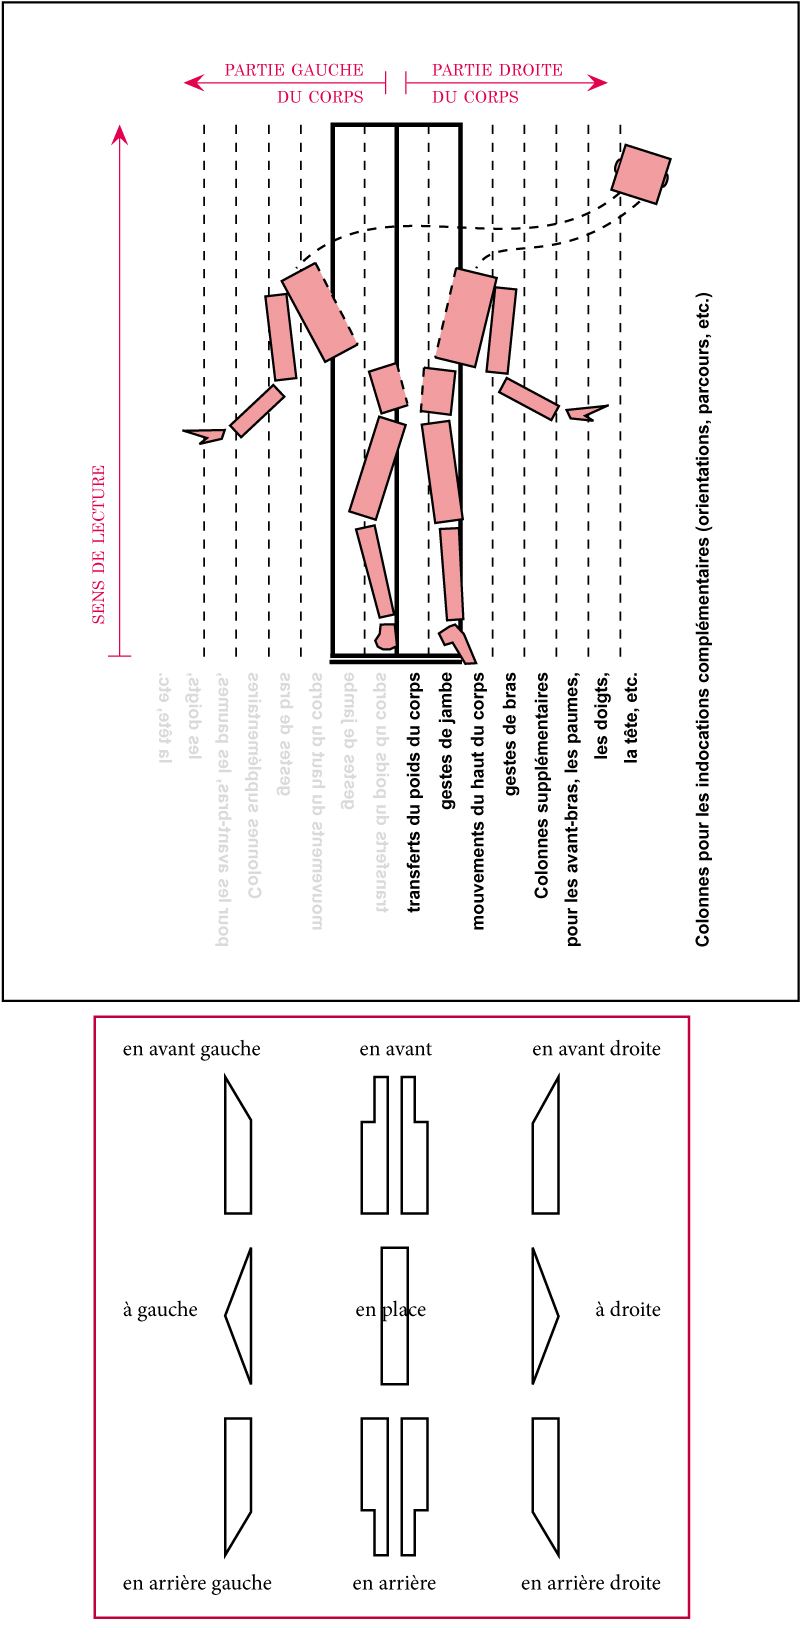
\includegraphics[width=\textwidth]{pictures/laban_partition_et_directions_cinetographie.png}
    \caption[Le système de partition de Laban]{Le système de partition de Laban. Ce système a été développé en premier lieu pour décrire les mouvements de danse. La lecture se fait de bas en haut, et chaque colonne correspond à une partie du corps. Dans chacune des colonnes, les indications de direction des parties du corps sont ajoutées. (Source: \parencite{WikiLaban})}
    \label{fig:laban_partition_et_directions_cinetographie}
\end{figure}

Aristidou \textit{et al.} proposent un ensemble de descripteurs caractérisant la danse folklorique selon quatre composantes du système de Laban, à savoir le corps, l'effort, la forme et l'espace \parencite{Aristidou2015FDE}. Les positions et les orientations, la hauteur du pelvis, la distance des jambes par rapport au sol et la taille des pas (distance entre les deux pieds) sont utilisés pour caractériser le corps. L'effort est divisé en quatre sous-catégories, possédants chacune deux polarités possibles : (i) l'espace occupé direct (précis et spécifique) ou indirect (non concentré sur un seul point), décrit à l'aide de l'orientation de la tête par rapport à la trajectoire du corps, (ii) le poids appliqué, fort ou léger, décrit à l'aide de la décélération du mouvement de la hanche, (iii) le temps, soudain (sentiment d'urgence, mouvement inattendu ou isolé) ou continu (réalisation du mouvement s'étalant dans le temps), décrit à l'aide de la vitesse et l'accélération du mouvement sur une période de temps prédéfinie, et (iv) le flux du mouvement, restreint (contrôlé, attentionné) ou libre (relâché, épanché, fluide), décrit à l'aide de la saccade du mouvement. La forme est décrite à l'aide du volume occupé par le corps de la personne, pris sur les cinq articulations extrêmes du corps (la tête, les mains et les pieds), la hauteur du torse, et la position des mains par rapport au corps. Enfin, l'espace est décrit à l'aide de la distance couverte par les hanches au court du temps, ainsi que l'aire correspondant à ce déplacement. L'organisation en quatre familles des descripteurs possède quelques similitudes avec la classification bas-niveau / haut-niveau qui est proposée dans les travaux de Larboulette et Gibet. Après extraction, les descripteurs de l'apprenant sont comparés avec ceux de l'expert, afin d'obtenir un score de corrélation correspondant à la similitude entre les deux gestes (Fig. \ref{fig:correlation_laban_descriptors}). Ce score, correspondant à la valeur absolue du coefficient de corrélation linéaire de Pearson, met en évidence les moments où le geste de l'apprenant est éloigné de celui de l'expert, mais ne propose pas une analyse sur les caractéristiques du mouvement à changer, malgré la précision des descripteurs utilisés. En conséquence, cette évaluation sous forme de score n'aide pas à l'amélioration de l'apprentissage du geste par l'apprenant.

\begin{figure}
    \centering
    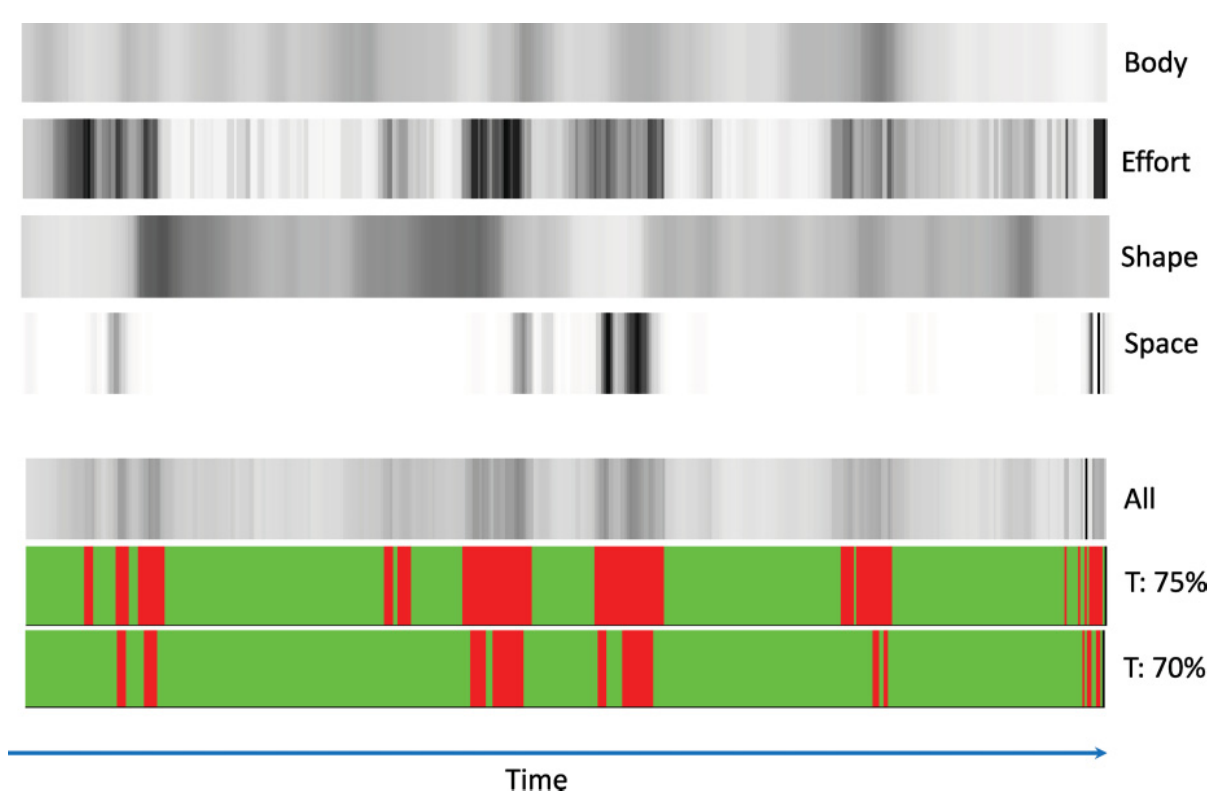
\includegraphics[width=\textwidth]{pictures/correlation_laban_descriptors.png}
    \caption[Corrélation entre le geste de l'apprenant et de l'expert]{La corrélation entre le geste de l'apprenant et de l'expert est calculée selon les quatre composantes du système de Laban considérées, puis moyennées. Le seuil $T$ choisi permet de changer la corrélation minimale à atteindre afin que le geste soit considéré comme bon. (Source: \parencite{Aristidou2015FDE}).}
    \label{fig:correlation_laban_descriptors}
\end{figure}

Toujours dans le domaine de la danse, Senecal \textit{et al.} utilisent un ensemble de descripteurs pour l'apprentissage de la salsa, selon trois axes : le rythme, l'interaction entre les partenaires et le style \parencite{Senecal2018MAa}. Ces descripteurs sont relatifs aux déplacements à effectuer lors de la danse. Ainsi, le rythme est évalué grâce à la position des pieds. Les valeurs successives de la norme de la vitesse des pieds attendues sont obtenues grâce à l'analyse du geste de l'expert. Le décalage entre les points d'inflexion de ce profil, correspondant à une nouvelle étape dans la suite de pas à réaliser, et ceux de l'apprenant permettent de mettre en évidence la synchronisation des pas avec la musique : un décalage temporel est ainsi obtenu. Le spectre du rythme de danse est ensuite extrait, à l'aide d'une transformée de Fourier, pour obtenir le décalage fréquentiel. L'interaction entre les partenaires est analysée sous trois angles : la corrélation du mouvement des jambes des deux partenaires, le décalage de rythme entre les deux partenaires, et enfin le décalage fréquentiel entre les deux partenaires. Enfin, le style est analysé à partir de l'aire couverte par la performance entière et la quantité de mouvement moyenne des hanches. Cette étude nécessite néanmoins d'extraire le tempo de la musique utilisée, dans le but d'obtenir un point de référence pour la synchronisation. Les descripteurs du mouvement sont donc complétés par une information temporelle supplémentaire non-relative au mouvement, celle des temps auxquels les percussions de la musique se font entendre. Ces données ne sont pas analysables sans connaissances en traitement du signal. Ainsi, il est impossible de présenter ces descripteurs sans une phase d'interprétation nécessaire pour tirer des conclusions sur le mouvement des apprenants. De plus, cette étude montre que malgré la sélection des descripteurs \textit{a priori} avec un expert, seuls quatre d'entre eux peuvent réelement aider à qualifier de manière satisfaisante le niveau des apprenants.

\subsection{Descripteurs pour l'indexation et la recherche de mouvements}
Les méthodes d'indexation et de recherche de mouvements cherchent à indexer les mouvements à l'aide de caractéristiques discriminantes, dans le but de de les stocker au sein d'une base de données. Le second objectif est de créer un langage de requête servant à retrouver et extraire efficacement et rapidement ces mouvement au sein d'une telle base de données.

Dans le cadre de la recherche de mouvements, Sakurai \textit{et al.} extraient un pentagone servant à représenter les postures du mouvement, à l'aide des données de position des articulations du squelette, dans l'optique de les comparer \textit{a posteriori} \parencite{Sakurai2015Ros}. Les données, capturées à l'aide d'une caméra Kinect™, sont prétraitées pour éliminer le bruit inhérent à ce type de capture. Ce traitement consiste à calculer, pour chaque posture, une moyenne sur les cinq postures adjacentes. Les postures sont ensuite normalisées, en harmonisant l'origine des repères, puis en divisant la longueur de chaque membre du corps par la taille du squelette. Un pentagone est ensuite extrait, reliant la tête, la main droite, le pied droit, le pied gauche et la main gauche. De ce polygone, trois aires différentes sont extraites, servant à représenter le mouvement (\ref{fig:polygons_areas}). La phase de recherche utilise ensuite l'algorithme de la Déformation Temporelle Dynamique (\textit{Dynamic Time Warping}, \textit{DTW}) pour calculer la distance entre le mouvement effectué et ceux présents au sein de la base de données. Cet algorithme permet de mesurer la similarité entre deux séries temporelles, ainsi que de les aligner, tout en s'affranchissant des contraintes temporelles. Plus formellement, l'algorithme du \textit{DTW} réalise un \textit{matching} entre les valeurs discrètes de deux séries temporelles. Si l'on prend l'exemple de deux personnes effectuant le même parcours, mais marchant à des vitesses différences,  la valeur du \textit{DTW} calculé entre ces deux séries temporelles sera élevée, indiquant une forte similitude entre ces deux séries, là où la distance euclidienne indiquera un écart élevé entre ces séries. Le mouvement stocké ayant la distance au sens du \textit{DTW} la plus petite est considéré comme étant le mouvement recherché. Afin d'évaluer les résultats, la métrique du \textit{F-score} est utilisée. Cette métrique est une combinaison de la Précision (P), qui correspond au ratio de de réponses correctes retournées par rapport au nombre total de réponses, et du Rappel (R), qui correspond au ratio de bonnes réponses retournées par rapport au nombre total de bonnes réponses. Les résultats des expérimentations montrent que, dans tous les cas, le descripteur basé sur les l'aire des quatre triangles extrait des mouvements enregistrés par la Kinect™ fourni le meilleur \textit{F-score}, par rapport aux deux autres descripteurs. Cette décomposition du mouvement en aires géométriques permet d'obtenir une performance de retour d'environ 71\% (au sens du \textit{F-Score}), environ 30\% plus faible que lors de l'utilisation de données capturées avec des systèmes de capture du mouvement plus précis. Les auteurs notent que cette différence peut être due à deux paramètres : la qualité des données obtenues (et donc, par extension, la méthode de filtrage appliquée) ainsi que le nombre d'aires extraites du polygone.

\begin{figure}
    \centering
    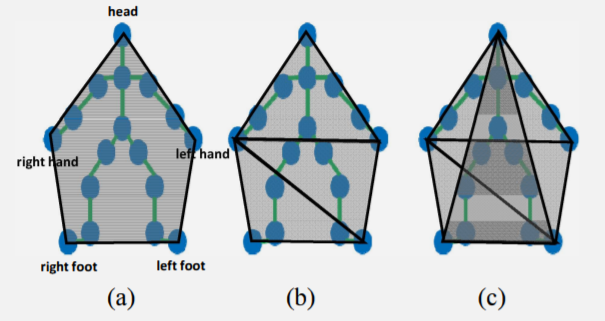
\includegraphics[width=\textwidth]{pictures/polygons_areas.png}
    \caption[Aires extraites du polygone du squelette \parencite{Sakurai2015Ros}]{Les trois descripteurs, constitués d'aires extraites du polygone englobant le squelette: (a) l'aire du polygone entier, (b) l'aire de trois polygones, (c) l'aire de quatre polygones (Source: \parencite{Sakurai2015Ros}).}
    \label{fig:polygons_areas}
\end{figure}

Xiao \textit{et al.} ont développé un système de descripteurs basés sur des postures 2D permettant de retrouver un mouvement à partir de dessins de postures-clés \parencite{Xiao2015Sbh}. Le mouvement est d'abord projeté sur 8 plans différents, de façon à passer d'une représentation 3D à plusieurs représentation 2D. Le système extrait ensuite des lignes reliant certaines articulations entre elles (les articulations extrêmes entre elles et les articulations extrêmes par rapport à la hiérarchie du squelette) servant à caractériser les articulations du corps à partir de leur distance relative, la direction de cette distance, la distance des articulations par rapport aux lignes et l'angle formé entre les différentes lignes (Fig. \ref{fig:skeletons_Xia}).

\begin{figure}[h]
    \centering
    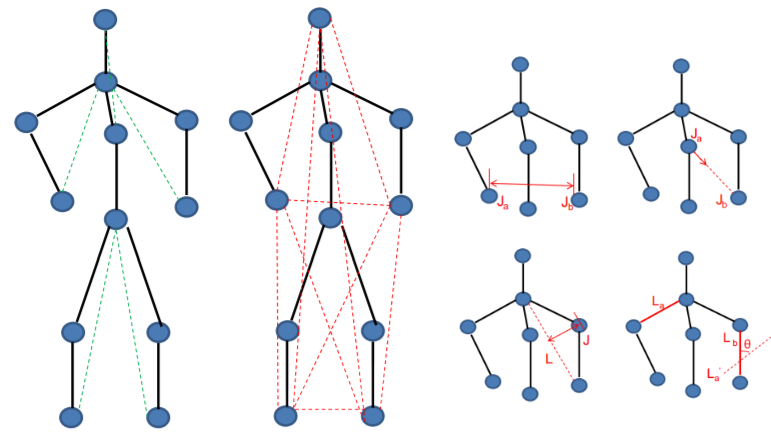
\includegraphics[width=\textwidth]{pictures/skeletons_Xia.png}
    \caption[Descripteurs basés sur les positions relatives des articulations entre elles \parencite{Xiao2015Sbh}]{Les descripteurs extraits caractérisent les postures par rapport aux distances relatives des articulations entre elles, ainsi qu'à leur distance et l'angle formé par rapport aux lignes reliant les autres articulations (Source: \parencite{Xiao2015Sbh}).}
    \label{fig:skeletons_Xia}
\end{figure}

Ces descripteurs sont ensuite réduits à un sous-ensemble, afin de limiter la redondance des informations contenues dans les données et d'améliorer les temps d'analyse \textit{a posteriori}. Pour cela, une méthode de sélection de caractéristiques semi-supervisée, basée sur le score Laplacien est utilisée. Ce score se base sur l'hypothèse que la projection des données dans un espace de caractéristiques réduits préserve la structure initiale de ces données \parencite{He2005LSf}. Le processus de recherche du mouvement se base sur un dessin fait à main levé par l'utilisateur. Le nombre de traits est limité à cinq, et le premier trait doit correspondre au torse. Grâce à ces contraintes, il est possible d'étiqueter automatiquement les articulations une fois le dessin terminé. La suite de postures dessinées par l'utilisateur est ensuite comparée à toutes les projections des mouvements présents dans la base de données à l'aide d'un algorithme des K plus proches voisins, et le mouvement le plus proche du dessin est récupéré (Fig. \ref{fig:posture_retrieval}).

\begin{figure}[h]
    \centering
    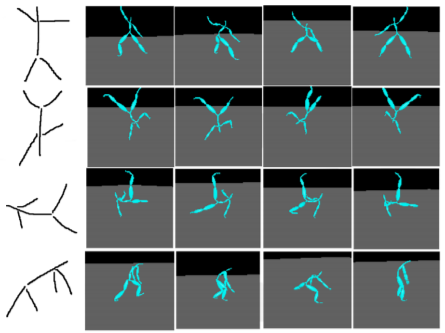
\includegraphics[width=\textwidth]{pictures/posture_retrieval.png}
    \caption[Mouvement retournés à partir de postures dessinées \parencite{Sakurai2015Ros}]{Quatre exemples de mouvement retournés à partir de postures dessinées à la main (Source: \parencite{Sakurai2015Ros}).}
    \label{fig:posture_retrieval}
\end{figure}

Les travaux cités ci-dessus proposent des ensembles de caractéristiques ayant pour but de stocker et de rechercher des mouvements de manière rapide et précise. Ces ensembles utilisent généralement une étape de sélection de caractéristiques, afin de réduire la dimensionnalité des données et ainsi d'accélérer le processus de recherche. Cette réduction peut cependant éliminer des descripteurs utiles à l'analyse du mouvement par un humain, et ainsi priver l'expert d'informations cruciales. En outre, la non prise en compte de l'utilisabilité, ni de la contextualisation de ces descripteurs par un humain fait que leur analyse peut être limitée en termes de retours possibles sur l'apprentissage d'un geste, voire impossible.


\subsection{Descripteurs pour la reconnaissance d'actions}
Certains travaux se focalisent sur l'extraction de descripteurs servant à identifier et séparer plusieurs actions. Dans ce cas, l'action peut soit concerner le corps entier (s'asseoir, prendre un objet, \textit{etc.}) ou des parties précises du corps (\textit{e.g.} reconnaissance d'écriture manuscrite).

 Ainsi, dans le cadre de la reconnaissance d'écriture, Delaye et Anquetil ont implémenté un ensemble de 49 descripteurs, nommé HBF49, liés à la manière d'écrire \parencite{Delaye2013HBF}. Ces descripteurs servent à caractériser les mouvements d'écriture, à l'aide : des points de début et de fin de trait, des angles formés par les différentes parties des lettres, de la proportion de trajectoires dirigées vers le bas, \textit{etc.} Cet ensemble de descripteurs a pour but de pallier les limites des ensembles de descripteurs existants pour l'écriture manuscrite. En effet, les travaux antérieurs ne permettent pas de caractériser toutes les informations pour ces gestes, car ils répondent souvent à un besoin d'observation et d'analyse précis, et aucune évaluation de référence n'a été conduite afin de les valider. Les tests effectués sur plusieurs jeux de données reconnus montrent que cet ensemble obtient un meilleur taux de reconnaissance de symboles que les jeux de descripteurs existants.

Dans le cadre de la reconnaissance d'actions, les travaux de Boulahia \textit{et al.} se basent en partie sur l'ensemble de descripteurs HBF49 et les généralisent à une trajectoire 3D dans l'environnement \parencite{Boulahia2016HIF}. Ces descripteurs ne posent aucune hypothèse sur les gestes considérés, et peuvent être utilisés pour n'importe-quel type de gestes. La validité de ce jeu de descripteurs pour décrire le mouvement, appelé HIF3D, a été testé sur deux jeux de données (HDM05 \parencite{HDM05Database} et UTKinect \parencite{UTKinectDatabase}) constitué de gestes non-techniques, et mis en concurrence avec d'autres ensembles de descripteurs déjà testés sur ces jeux de données (\textit{e.g.} SMIJ, Cov3DJ, HOJ3D). Il en ressort que les résultats sont meilleurs avec le jeu de descripteurs HIF3D.

Rao \textit{et al.} utilisent les moments d'inflexion dans la trajectoire, appelés instants dynamiques, afin de proposer une représentation des changements de trajectoire du geste, permettant ainsi de les segmenter en unités élémentaires \parencite{Rao2002VRR}. Les gestes utilisés dans l'étude sont des gestes du quotidien, \textit{e.g.} ouvrir et fermer un placard, prendre un objet, le poser, \textit{etc.} Ces unités élémentaires sont ensuite utilisées pour associer d'autres parties du mouvement, ou d'autres mouvements, à cette action. Ainsi, le système peut ensuite soit reconnaître une unité élémentaire comme étant similaire à une des unités élémentaires déjà visualisée, ou alors créer une nouvelle unité élémentaire si jamais celle-ci n'est pas suffisamment semblable à celles présentes dans le corpus. Cependant, la méthode ne se basant sur aucun apprentissage ou modèle pour segmenter et reconnaitre les mouvements, aucune sémantique n'est associée aux groupes d'unités élémentaires ainsi obtenus.


Des ensembles de descripteurs tel que HIF3D proposé par Boulahia \textit{et al.} couvrent beaucoup d'aspects différents du geste, offrant ainsi un bon taux de reconnaissance des actions. L'intégration de ces descripteurs à un système limite les besoins de réingénierie dans le cas de multiple domaines applicatifs, car il sont pensés pour être capable de reconnaitre une grande variété de mouvements. Cependant, beaucoup de ces travaux ne se focalisent pas sur l'apprentissage humain de mouvements. Ainsi, l'utilisation de ces descripteurs en tant qu'information descriptive humainement interprétable n'est pas prise en considération. Il n'est pas assuré que les descripteurs soient utilisables dans un processus d'analyse par un expert du geste ne disposant pas de connaissances scientifiques spécifiques à ces descripteurs.
%Le domaine de l'analyse de mouvement avec des données vidéo est également très riche en publications. Les descripteurs extraits à partir de vidéos peuvent être les mêmes que ceux extraits de données 3D; cependant, les méthodes de calcul ne sont pas les mêmes.

%En se basant sur les travaux de Laban, \parencite{Camurri2004AoE} proposent un système capable d'extraire une collection de descripteurs à partir d'enregistrements vidéo de mouvements. Le système permet de suivre le mouvement en temps réel et d'en extraire des descripteurs, mais également d'analyser la position occupée dans l'espace par la personne réalisant le geste, ainsi que l'extraction de trajectoires 2D à partir de la vidéo. Les descripteurs extraits des vidéos peuvent concerner des informations bas-niveau (trajectoire, vitesse, accélération) comme des informations haut-niveau (quantité de mouvement, orientation des parties du corps), selon la classification de Larboulette et Gibet \parencite{larboulette2015Descriptors}.

%Le domaine de l'étude de l'émotion chez l'humain utilise également de manière intensive des descripteurs, souvent extrait à partir du visage des personnes. Les émotions peuvent se lire à partir de plusieurs modalité du corps, mais les expressions faciales restent le moyen le plus efficace de les déterminer. Les travaux de \parencite{Ekman1978Fac} ont permis de créer le FACS (Facial Action Coding System), un ensemble de mouvements caractéristiques du visage, permettant de décomposer le mouvement en descripteurs. Ces descripteurs concernent les contractions (et décontractions), et sont appelés AU (action units). Ces descripteurs permettent de reconnaitre plusieurs émotions : la joie, la surprise, la tristesse, la colère, le mépris et le dégoût.

%Il est possible d'utiliser ces descripteurs dans un processus de classification, avec ou sans réduction de dimensionnalité \parencite{SanchezMendosa2015Erf}. Il est également possible d'obtenir des informations sur l'émotion à partir de descripteurs provenant du corps entier tels que la fluidité du geste, l'extension spatiale, la quantité de mouvement, \textit{etc.} reliés au niveau d'activation (dynamique de l'émotion) et d'évaluation (posititivé ou négativité) du geste \parencite{Malatesta2016Age}.


\subsection{Discussion}
Les travaux portant sur la classification des descripteurs ont pour but de créer des familles, afin de corréler chacune d'entre elles à un type d'analyse voulue. Ces classifications présentent des différences dans leur méthode de discrimination. Ainsi, Larboulette et Gibet \parencite{larboulette2015Descriptors} s'intéressent d'avantage à la séparation des descripteurs en termes d'origine des descripteurs : les descripteurs concernant la cinématique, la dynamique et la géométrie, calculés à partir du mouvement brut, sont dits de bas-niveau, et les descripteurs calculés à partir de descripteurs bas-niveaux sont dits de haut-niveau. Chez Morel \cite{Morel2017Mts}, la considération première est de séparer les descripteurs en fonction de l'objet en mouvement considéré. Ainsi, la première famille concerne les descripteurs représentant un corps humain en mouvement, la deuxième contient les descripteurs déterminant la dynamique d'un objet en mouvement, et la troisième contient les descripteurs concernant des points précis de l'objet considéré. Aristidou et Chrysanthou proposent une classification en fonction de la caractéristique du mouvement à considérer, entre le mouvement, l'effort, l'espace et la forme \parencite{Aristidou2014Fef}. Dans tous les cas, l'explicabilité des descripteurs calculés et l'utilisation de ces valeurs par des personnes expertes ou non n'est pas considérée. Ainsi, un expert du mouvement sans connaissances scientifiques poussées et un apprenant supposé novice dans le domaine ciblé ne pourront faire un usage direct de ces indicateurs.

Les travaux se focalisant sur un ensemble précis de descripteurs permettent de décrire les aspects du geste considérés dans l'étude \parencite{Senecal2018MAa} \parencite{Aristidou2015FDE} \parencite{Delaye2013HBF}. Ces ensembles offrent une analyse précise : par exemple, dans le cadre de l'écriture manuscrite, seront considérés non seulement la position de début et de fin de la main, mais également les différents traits effectués, les inflexions du poignet, le nombre de trait allant de haut en bas, \textit{etc.}. Les descripteurs présents dans ces études ont souvent une application limitée dans des contextes autres que le cadre applicatif choisi, bien que certains ensembles aient été pensés afin d'être réutilisable dans d'autres contextes \parencite{Boulahia2016HIF}. Quelque-soit la portée des descripteurs calculés,ils sont proposés soit à des systèmes d'analyse automatique \parencite{Aristidou2015FDE}, soit à des experts à-même d'en extraire des informations pertinentes dans le cadre de la réalisation ou l'apprentissage d'un geste \parencite{Senecal2018MAa}. Ainsi, la facilité d'utilisation de ces descripteurs par un non-expert n'est pas garantie, voire peu probable, comme dans les travaux de Senecal \textit{et al.} par exemple\parencite{Senecal2018MAa}.

L'utilisation des classifications et ensembles de descripteurs proposés dans des contextes annexes n'est pas assurée. En effet, bien que certains travaux proposent des ensembles pouvant couvrir une large gamme de caractéristiques du mouvement, dans le but de faire de la reconnaissance automatique, l'utilisation de ces descripteurs dans une situation d'apprentissage n'est pas considérée. Il en va de même pour les travaux portant sur l'indexation et la recherche de mouvements proposant des ensembles de descripteurs adaptés à ces deux fonctionnalités. De plus, les travaux portant sur l'indexation et la recherche de mouvements au seins de bases de données proposent des ensembles de descripteurs dont l'utilisabilité par un humain n'est pas considéré \parencite{Sakurai2015Ros} \parencite{Xiao2015Sbh}. En outre, ces ensembles peuvent présenter des redondances sémantiques, soit entre eux, soit au sein même du jeu de descripteurs considéré. Le calcul des descripteurs est une tâche qui peut prendre un temps non-négligeable, en fonction du nombre de données à traiter. La réduction des redondances au sein de ces jeux de descripteurs et la prise en compte des capacités de perception et d'interprétation des acteurs de l'apprentissage sont trois éléments importants à prendre en compte pour la conception d'un EIAH dédié à l'apprentissage de geste. La prochaine section propose une classification d'un ensemble de descripteurs réduit, issus de travaux présentés dans cette section, décrivant les différentes caractéristiques d'un mouvement. Cette nouvelle classification propose des cas d'usages et des domaines d'application, ainsi que les connaissances scientifiques nécessaires (ou non à leur utilisation).

\section{Classification de descripteurs élémentaires}\label{sec:class_descr}
Une nouvelle classification répondant à des besoins d'observation et d'analyse variés est proposée dans cette partie. Nous ne présentons ici que des descripteurs dit élémentaires, c'est-à-dire des descripteurs qui ne sont pas issus d'un calcul, d'une réinterprétation ou d'un ensemble de descripteurs « bas-niveau » du mouvement. Par exemple, Aristidou et Chrysanthou \parencite{Aristidou2014Fef} définissent la « hauteur de la hanche » comme descripteur. Cependant, ce descripteur provient de la composante verticale du descripteur « position 3D » de la hanche : Dans ce cas, le descripteur dit élémentaire est celui de la position selon l'axe vertical.

Chaque descripteur est caractérisé par son appartenance à une ou plusieurs des familles présentes dans le tableau \ref{descriptors_family}. Cette classification s'inspire des classifications déjà établies dans les travaux cités précédemment \parencite{larboulette2015Descriptors} \parencite{Morel2017Mts}. Les différentes familles proposées ne sont pas exclusives. De plus, la nécessité de posséder des connaissances scientifiques pour pouvoir contextualiser et interpréter le descripteur est indiquée, afin de donner des pistes quant à l'utilisation de ces descripteurs dans des contextes de retour à l'expert ou à l'apprenant.

Les colonnes « non-contigu, contigu et global » permettent de donner la possibilité d'obtenir la ou les valeurs du descripteur respectivement(i) sur des points précis (postures-clés), (ii) sur des postures qui se suivent temporellement ou (iii) sur la totalité du mouvement. Dans le premier et le deuxième cas, un vecteur de valeurs correspondant à un descripteur est retourné, dont la taille correspond soit au nombre de posture-clés, soit au nombre de postures successives choisies, et dans le dernier cas, un seul descripteur caractérisant l'ensemble du mouvement sera obtenu.

Les colonnes « cinématique » et « géométrique » donnent une indication sur la provenance du descripteur : un descripteur cinématique est directement dérivé à partir des propriétés du mouvement, alors qu'un descripteur géométrique proposera une information sur des aspects spatiaux du corps, voire son environnement.

La colonne « utilisation courante » met en évidence des domaines où ce descripteur est couramment utilisé, donnant ainsi des pistes quant à l'utilisation d'un descripteur en fonction du contexte applicatif fourni.

Enfin, la colonne « connaissance scientifique requise » indique si l'analyse de ce descripteur par un humain nécessite de posséder des connaissances scientifiques adéquates, ou si, à l'inverse, il est possible pour une personne sans connaissances particulières de comprendre et de tirer des informations utiles pour l'apprentissage du geste à partir de la valeur de ce descripteur.

Un même descripteur élémentaire présenté dans le tableau ci-dessus peut exprimer différentes caractéristiques d'un mouvement, en fonction de la fenêtre temporelle considérée. Ainsi, la vitesse prise sur un intervalle défini permet de suivre l'évolution de cette dernière lors d'un effort particulier, alors que la vitesse moyenne du mouvement prise globalement (moyenne des vitesses instantanées) donne une indication sur la rapidité du mouvement général. L'analyse de la position à un moment donné indique dans quelle position l'apprenant se trouve, alors que l'analyse de l'évolution de la position sur un temps donné résulte en l'obtention de la trajectoire de l'apprenant.

Le sens d'une partie des descripteurs proposés dans le tableau \ref{descriptors_classif} est explicité ici :

\begin{itemize}
	\item mouvement saccadé : donne une indication sur la fluidité du mouvement
	\item courbure : mesure la vitesse de changement de la trajectoire
	\item quantité de mouvement : moyenne pondérée des vitesses d'un ensemble d'articulation du corps
	\item forme englobante : plus petite forme (boîte, sphère, ellipsoïde...) englobant la totalité des articulations et des membres du corps
	\item enveloppe convexe : enveloppe minimale englobant le corps (Voir Fig. \ref{fig:convex_hull})
	\item centre de masse : moyenne pondérée (ou non) des positions des articulations (ou d'un sous ensemble des articulations) du corps
	\item équilibre : valeur booléenne indiquant si la projection du centre de masse au sol est comprise au sein de la projection au sol de la forme englobante du corps
	\item profilage : décrit l'évolution de la forme du corps au cours du mouvement : extension/rétractation, élargissement/réduction, enflement/creusement
	\item quantité d'effort : caractérise l'intensité d'un effort fourni sur un intervalle de temps défini, variant de « faible » à « intense »
	\item durée d'effort : représente la durée d'un effort fourni, caractérisé en « urgent » ou « continu »
\end{itemize}

\begin{figure}[h]
    \centering
    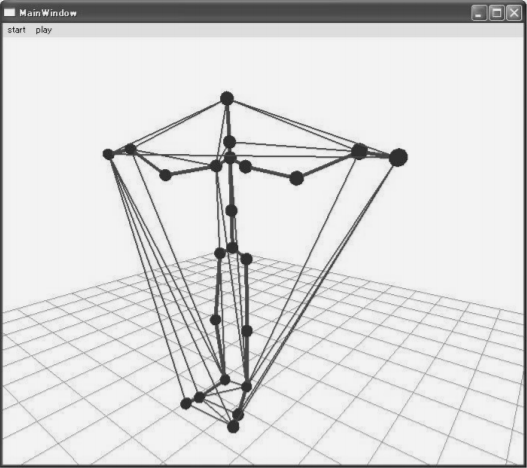
\includegraphics[width=6cm]{pictures/convex_hull.png}
    \caption[Enveloppe convexe]{L'enveloppe convexe correspond à la forme qui englobe le corps dans sa totalité, tout en gardant la distance minimale pour chaque segment la composant (Source: \parencite{Hachimura2005Aae})}
    \label{fig:convex_hull}
\end{figure}


\begin{landscape}
\centering
\begin{table}[]
\begin{tabular}{|l|l|l|}
\cline{1-3}
Type de descripteur & Description & Exemple \\ \cline{1-3}

Non contigu & \makecell[l]{calculé à des moments précis du mouvement\\(une ou plusieurs valeurs)} & Orientations prises à des postures clés\\ \cline{1-3}

Contigu & \makecell[l]{calculé sur une suite de postures contigües\\ (possiblement le mouvement entier)} & Vitesse au court du temps \\ \cline{1-3}

Global & \makecell[l]{une unique valeur qui définit une caractéristique du mouvement\\sur toute sa durée (une seule valeur)} & \makecell[l]{Périodicité du\\mouvement} \\ \cline{1-3}

\makecell[l]{Cinématique} & \makecell[l]{caractérise les aspects du mouvement relatifs au déplacement,\\la rotation, la vitesse, etc.                                                        } & Vitesse moyenne du mouvement\\ \cline{1-3}

Géométrique & \makecell[l]{caractérise des aspects relatifs aux parties du corps\\par rapport au corps tout entier ou à l'environnement} & \makecell[l]{Boîte englobante}\\ \cline{1-3}

\makecell[l]{Utilisation\\courante} & \makecell[l]{si un descripteur est souvent utilisé dans un domaine\\applicatif particulier} & \\ \cline{1-3}

\makecell[l]{Connaissance\\scientifique requise} & \makecell[l]{indique si le descripteur requiert des connaissances\\ scientifiques (physique, mécanique, géométrique, etc.) ou non\\pour être compris et utilisé dans un contexte particulier} & \\ \cline{1-3}
\end{tabular}
\caption[Différentes familles de descripteurs]{Différentes familles de descripteurs. Elles proviennent des travaux de Larboulette et Gibet \parencite{larboulette2015Descriptors} et Morel \parencite{Morel2017Mts}.}
\label{descriptors_family}
\end{table}
\end{landscape}

\begin{landscape}
\renewcommand{\arraystretch}{1.5}
\begin{table}[]
{\footnotesize
\begin{tabular}{c||c|c|c|c|c|c|c}
Descripteur & Contigu & Non-contigu & Global & Cinématique & Géométrique & \makecell[c]{Utilisation\\courante} & \makecell[c]{Connaissance\\scientifique\\requise} \\\hline
Position & X & X & & X & & Polyvalent & Géométrie \\\arrayrulecolor{gray}\hline
Orientation & X & X & & X & & Polyvalent & Géométrie \\\arrayrulecolor{gray}\hline
Durée & & & X & X & & Polyvalent & Non \\\arrayrulecolor{gray}\hline
\makecell[c]{Distance\\effectuée} & X & & X & & X & Polyvalent & Non \\\arrayrulecolor{gray}\hline
Vitesse & X & X & X & X & & Polyvalent & Cinématique du mouvement \\\arrayrulecolor{gray}\hline
Accélération & X & X & X & X & & Polyvalent & Cinématique du mouvement \\\arrayrulecolor{gray}\hline
\makecell[c]{Mouvement\\saccadé} & X & X & & X & & Analyse de la performance & Cinématique du mouvement\\\arrayrulecolor{gray}\hline
Courbure & X & X & & X & & Reconnaissance d'actions & Géométrie \\\arrayrulecolor{gray}\hline
\makecell[c]{Quantité\\de mouvement} & X & X & X & X & & Analyse de la performance & Dynamique du mouvement \\\arrayrulecolor{gray}\hline
Forme englobante & X & X & X & & X & Polyvalent & Géométrie \\\arrayrulecolor{gray}\hline
Enveloppe convexe & X & X & X & & X & Indexation et recherche & Géométrie \\\arrayrulecolor{gray}\hline
Centre de masse & X & X & X & & X & Analyse de la performance & Dynamique du mouvement \\\arrayrulecolor{gray}\hline
Équilibre & X & X & X & & X & Analyse de la performance & Non \\\arrayrulecolor{gray}\hline
Profilage & X & X & X & & X & Analyse de la performance & Dynamique du mouvement \\\arrayrulecolor{gray}\hline
Quantité d'effort & X & X & X & X & & Analyse de la performance & Dynamique du mouvement \\\arrayrulecolor{gray}\hline
Durée d'effort & X & & X & & & Analyse de la performance & Non
\end{tabular}
}
\caption[Classification des descripteurs élémentaires]{Une classification des descripteurs élémentaires de la littérature. Ils proviennent des travaux de Larboulette et Gibet \parencite{larboulette2015Descriptors} et Morel \parencite{Morel2017Mts}.}
\label{descriptors_classif}
\end{table}
\end{landscape}

En réduisant ainsi les descripteurs à un ensemble élémentaire, il est possible d'exprimer les descripteurs de plus haut-niveau par une combinaison de ces descripteurs. L'utilisation de cet ensemble pourrait ainsi, à terme, mener à la création d'un système de conception et d'intégration de descripteurs de haut niveau, calculables à partir des descripteurs élémentaires proposés et inteprétables par l'usager en fonction du contexte et de ses connaissances.



\section{Discussion}
Dans ce chapitre , nous avons étudié les descripteurs du mouvement calculables à partir des données capturées en fonction de leurs usages et des objectifs d’analyse. À partir de données de positions et d'orientations décrivant le mouvement de manière précise, il est possible d'extraire des informations caractérisant la forme, la position, la dynamique ou la cinématique du corps humain et du mouvement qui lui est associé. Il existe beaucoup de descripteurs pour caractériser le geste \parencite{larboulette2015Descriptors}. Cependant, ils sont majoritairement issus des descripteurs élémentaires présentés dans le tableau \ref{descriptors_classif}, soit d'une combinaison de plusieurs de ces descripteurs. Ainsi, il est en conséquence possible de réduire la large gamme de descripteurs utilisés dans l'analyse du mouvement à l'ensemble élémentaire présenté ici. L'utilisabilité de ces descripteurs par une personne non-experte, ainsi que les domaines applicatifs dans lesquels ils sont le plus souvent utilisés, sont considéré, afin de faciliter le choix des descripteurs en fonction des contextes applicatifs. L'implémentation de cet ensemble élémentaire au sein d'un système dédié à l'analyse de gestes permettrait de couvrir les besoins d'observations et d'analyse des utilisateurs, soit en calculant et en utilisant directement ces descripteurs, soit en combinant certains d'entre eux dans le but d'obtenir de nouveaux descripteurs.

Bien qu'il soit possible d'extraire ces descripteurs à partir de données de mouvement, ils ne sont néanmoins pas tous utiles en fonction du contexte. Ainsi, la pertinence des indicateurs est définie par les besoins d'observation et d'analyse des experts ou apprenants. La formalisation des besoins d'observation et d'analyse en descripteurs calculables est une étape cruciale afin de proposer des indications utiles sur le geste. Cette formalisation peut mener à la proposition d'un ensemble de descripteurs pertinent dans le cadre de l'analyse d'un mouvement. La problématique de formalisation de nouveaux descripteurs dans un système existant est rarement prise en compte dans les travaux existants. Cela peut s'expliquer par le côté \textit{ad-hoc} des systèmes extrayant des descripteurs du mouvement d'une part, et par la non-contextualisation des classifications de descripteurs d'autre part.

Il faut noter que le niveau de connaissance requis pour l'analyse des descripteurs est également lié au contexte. Ainsi, si l'on prend l'exemple d'une course à pied, le calcul et l'analyse conjointe de la durée et de la distance effectuée peuvent être suffisantes pour le pratiquant non spécialiste en biomécanique pour estimer sa performance physique. À l'inverse, l'analyse de la quantité d'effort ainsi que la durée de cet effort pour une partie précise du corps pourra être utilisée par un médecin afin d'évaluer les risques de blessures, mais sera difficile à interpréter pour une personne non-experte. L'analyse de ces données doit se faire dans un contexte précis, par un expert humain ou un système où la connaissance experte a été intégrée, pour être en mesure de donner du sens aux valeurs ainsi obtenues. Le prochain chapitre montre les différentes méthodes et techniques d'analyses possibles à partir de données de mouvement et des descripteurs.

\chapter{Analyse du mouvement capturé}
Dans ce chapitre, nous explorons les différentes manières d'analyser le mouvement. En particulier, l'analyse du mouvement humain, dans le contexte d'un apprentissage ou de l'amélioration d'un geste, a principalement deux objectifs non exclusifs : (i) l'apprentissage ou l'amélioration du geste en lui-même, par imitation d'une succession de postures dans le temps ou par reproduction de ses principales caractéristiques (extraites de manière automatique ou non) et (ii), l'apprentissage ou l'amélioration de propriétés du ou des objets manipulés par l'intermédiaire du geste appris (manipulation d'un scalpel lors d'une procédure chirurgicale, par exemple).

L'apprentissage du geste par observation et imitation de démonstrations peut être qualifié de naturelle, simple à mettre en œuvre mais peu efficace sans un grand nombre d’itérations du processus « démonstration-imitation » \parencite{Yang2014RoP}. Le savoir de l'expert permet le plus souvent de juger de la qualité du geste effectué. Ce regard expert sur le geste peut conduire à des propositions d'améliorations, sous la forme d'entraînements relatifs aux défauts du geste effectué. Les observations et l'analyse de l'expert sont cependant limitées par la complexité du geste : un geste qui fait intervenir, rapidement, de nombreuses parties du corps peut être difficile à analyser dans son intégralité, comme pour la danse par exemple \parencite{Kyan2015ABD}. Il est possible de pallier cette difficulté en analysant le mouvement capturé. En effet, l'utilisation de données de mouvements capturés permet d'avoir une représentation visualisable à volonté, selon différentes vitesses de lecture, sous différents angles de vue \parencite{Yoshinaga2015Doa} et permet également d'utiliser des processus automatiques afin d'aider cette analyse à l'aide de : calculs de descripteurs, détections d'une séquence ordonnée d'actions, l'utilisation de techniques d'apprentissage automatique ou la réduction des données. Les parties suivantes présentent différentes méthodes existantes pour l'analyse des gestes tout en positionnant l'usager et ses contributions (apprenant ou enseignant) au sein de chacune d'elle. Ces catégories ne sont pas exclusives, c'est-à-dire qu'un même système dédié à l'apprentissage de mouvement peut se trouver à l'intersection de deux catégories ou plus.

\section{Analyse du geste par observation humaine}
Cette section présente plusieurs études où l'analyse du geste est faite de manière empirique par un humain. Cette analyse peut directement s'effectuer par visualisation du mouvement, ou à l'aide de métriques calculées en fonction des besoins d'observations. Dans les deux cas, les données doivent être analysées par un humain dans un premier temps et les retours sont systématiquement délivrés par un expert à un apprenant.

Le domaine médical est un domaine qui nécessite non seulement de pouvoir étudier la motricité du patient, mais aussi son état physiologique. À l'aide d'un ensemble de capteurs hétérogène (réduit \parencite{Alankus2010TCG} ou non \parencite{deVries2006Cro}), il est possible d'obtenir suffisamment d'informations pour que le médecin soit capable de délivrer un verdict. Bien que de nombreux types de capteurs existent pour l'analyse médicale, nous nous concentrons ici sur les capteurs permettant d'obtenir des données relatives aux mouvements, et non des indications sur l'état physiologique du patient (capteur cardiaque, par exemple).

L'analyse de la démarche fait un usage intensif des données de mouvements capturés \parencite{Chen2016TPG}. Cette analyse permet d'évaluer le résultat de nombreuses procédures médicales chez un patient : pose de prothèse, chirurgie, rééducation, mais également le suivit de l'évolution de la posture, ainsi que les risques de chute, notamment chez les personnes âgées. Ainsi, il est crucial d'obtenir des données correspondant aux besoins d'observation et d'analyse des médecins (Fig. \ref{fig:gait_possibilities}). De tels descripteurs peuvent être extraits à partir d'un squelette 3D.

\begin{figure}
    \centering
    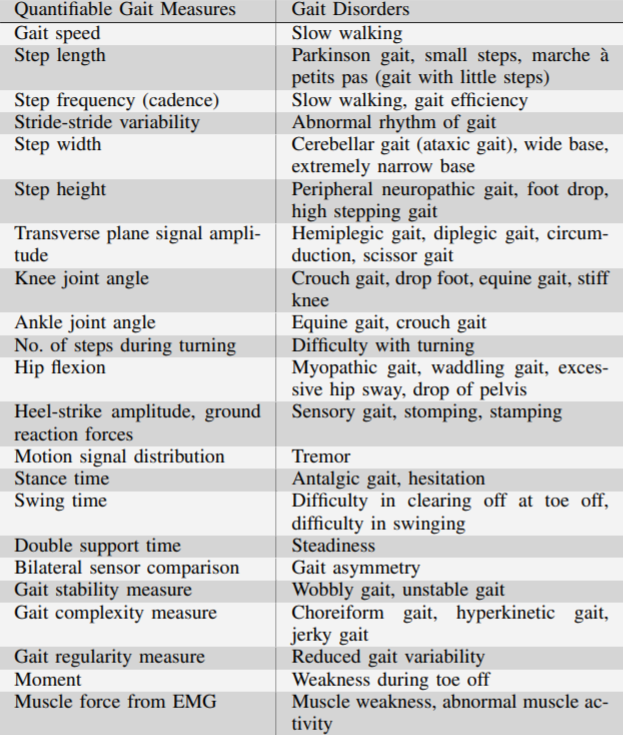
\includegraphics[width=9cm]{pictures/gait_possibilities.png}
    \caption[Descripteurs pour l'analyse de la démarche \parencite{Chen2016TPG}]{Des exemples de descripteurs extractibles relatifs à la démarche possible et leurs applications pour la détection de pathologies \parencite{Chen2016TPG}.}
    \label{fig:gait_possibilities}
\end{figure}

La chirurgie gagne beaucoup à utiliser les casques de réalité virtuelle afin de simuler des procédures dans un environnement clinique d'apprentissage. En effet, il n'est pas envisageable de s'entraîner sur de vrais patients \parencite{Kneebone2004Sac}. Ainsi, l'utilisation d'environnements virtuels, combinés par exemple à des processus de gamification \parencite{Pulijala2017VRS}, permet d'entraîner plus de chirurgiens en parallèle, ainsi que de permettre une vérification des acquis sans risque. Dans les travaux de Choi \textit{et al.} \parencite{Choi2015103}, l'utilisation conjointe de retours visuels en temps réel, ainsi que d'indicateurs calculés par rapport à la tâche à effectuer (temps de la procédure, force appliquée, etc.) permet de proposer une visualisation de la performance.

Le sport est un domaine où l'apprentissage du geste est au coeur de la formation. Il est nécessaire de pouvoir évaluer à la fois le résultat du geste, mais également la manière dont il est fait, afin d'éviter des risques de blessure \parencite{Rawashdeh2016WIMU}. L'utilisation d'experts virtuels est une des possibilités offertes par la capture de mouvements. Bien que ces systèpmes permettent parfois de s'affranchir de la présence d'un expert, ils ne présentent pas systématiquement une amélioration de l'apprentissage par rapport aux méthodes d'enseignement traditionnelles \parencite{Philo2003Tfp}.

Pour l'apprentissage du karaté, le système développé par Burns \textit{et al.} propose un environnement en réalité virtuelle \parencite{Burns2011Uvh}. L'apprenant doit, au fur et à mesure des séances, reproduire à l'identique les gestes de l'expert. Les sessions sont divisées en deux parties : une partie sur l'explication du geste à effectuer, fournie à l'aide d'une vidéo de l'expert effectuant le mouvement et une autre sur des exercices relatifs au geste. L'expert y est représenté sous forme 3D dans un environnement virtuel correspondant à un dojo (Fig. \ref{fig:Burns_karate}). L'évaluation est réalisée par l'expert, une fois au début de l'apprentissage et une fois à la fin, en analysant les vidéos des gestes des apprenants. Ces enregistrements sont réalisés hors du contexte virtuel. L'expert évalue les gestes des apprenants en attribuant un score, en fonction du degré de similitude du geste de l'apprenant par rapport à celui de l'expert. Les résultats montrent que l'avatar virtuel est aussi efficace qu'un expert réel pour l'apprentissage de ces gestes.

\begin{figure}
    \centering
    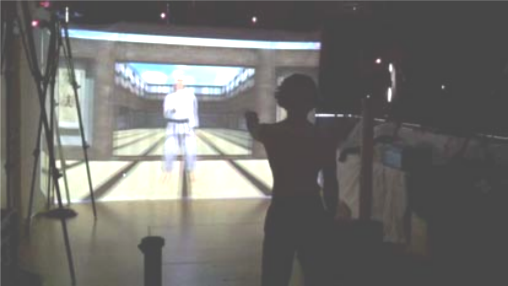
\includegraphics[width=\textwidth]{pictures/Burns_karate.png}
    \caption[Environnement virtuel pour l'apprentissage du karaté \parencite{Burns2011Uvh}]{L'environnement virtuel pour le Karaté proposé par Burns \textit{et al.} est utilisé pour l'entrainement de l'apprenant. L'évaluation est faite de manière qualitative par un expert \textit{a posteriori} \parencite{Burns2011Uvh}.}
    \label{fig:Burns_karate}
\end{figure}

Le système développé par Le Naour \textit{et al.}, présenté dans le chapitre 2, permet d'aider à l'apprentissage de mouvement en superposant le modèle de l'expert à celui de l'apprenant au sein d'un environnement virtuel \parencite{LeNaour2019S3V}. Le cas de test utilisé était celui du lancer au football américain. À partir d'une démonstration effectuée par l'expert, l'apprenant doit ensuite effectuer une suite de plusieurs lancers, à partir desquels sont calculés la valeur de l'écart-type du \textit{DTW} entre les mouvements de l'apprenant et de l'expert, ainsi que la distance du lancer par rapport au centre de la cible visée. Le groupe ayant reçu la visualisation du mouvement de l'apprenant superposé à celui de l'expert comme retour a montré une amélioration plus importante du geste que les groupes ne l'ayant pas obtenu.

À l'inverse, Kora \textit{et al.} ont proposé un environnement en réalité augmentée permettant l'apprentissage du golf en autonomie \parencite{Kora20151559}. La projection du modèle de l'expert dans un casque porté par l'apprenant, superposé au squelette (capté à l'aide d'une Kinect) de la personne faisant le geste, permet d'aider l'apprenant à corriger son geste au fur et à mesure de l'entraînement. L'apprenant est en auto-évaluation : aucune indication ne lui est fournie, c'est donc à lui d'être capable d'évaluer seul les changements à apporter à son geste afin de parfaire le mouvement du swing.

Des systèmes se basent sur la superposition des données de l'apprenant avec celles des experts afin de proposer une correction par mimétisme \parencite{Yoshinaga2015Doa}. Dans ces cas, le mouvement de l'apprenant est rejoué par dessus celui de l'expert, et les corrections peuvent s'effectuer par rapport au décalage temporel ou spatial de l'apprenant par rapport à l'expert.
Le système proposé par Yoshinaga et Soga, testé sur l'archerie japonaise, permet d'agréger plusieurs modèles experts afin de proposer soit un expert au choix, soit l'expert le plus proche de l'étudiant morphologiquement parlant, soit une moyenne des experts ou soit l'expert médian (c'est-à-dire l'expert le plus proche de la moyenne des experts) \parencite{Yoshinaga2015Doa}. Cette approche permet de limiter les différences morphologiques, dans le cas où un des modèles experts est semblable à celui de l'apprenant. La comparaison du geste de l'apprenant à celui de l'expert est réalisée à l'aide d'une correspondance en programmation dynamique : ainsi, le mouvement est représenté de façon amorphologique, et il est possible de faire correspondre les mouvements temporellement, même en présence de variations de timing, vitesse et d'amplitude des mouvements. Il est possible d'utiliser ce système soit en autonomie, soit à l'aide d'un expert qui analysera le geste de l'apprenant. Dans ce cas, l'expert peut être en mesure d'expliquer les différences entre le geste de l'apprenant et celui des modèles d'experts, ajoutant ainsi son expertise au retour visuel (Fig. \ref{fig:Yoshiniga_archery}).

\begin{figure}
    \centering
    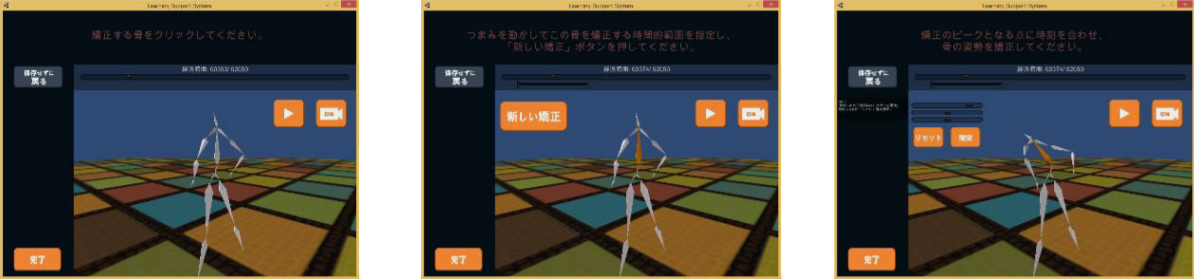
\includegraphics[width=\textwidth]{pictures/Yoshiniga_archery.png}
    \caption[Correction du mouvement de l'apprenant \parencite{Yoshinaga2015Doa}]{L'environnement proposé par Yoshinaga \textit{et al}. permet à l'expert de modifier directement les positions et les orientations des membres du corps de l'apprenant sur l'enregistrement du geste originel, afin de lui proposer des corrections à distance \parencite{Yoshinaga2015Doa}.}
    \label{fig:Yoshiniga_archery}
\end{figure}



\section{Analyse par observation d'indicateurs calculables du geste}
L'explication des caractéristiques d'un geste, ainsi que son évaluation, peut varier en terme de précision, en fonction du contexte applicatif mais également de la possibilité d'expliciter et de formaliser les caractéristiques importantes en descripteurs calculables. Dans le cas où les caractéristiques du geste à réaliser, ainsi que les propriétés biomécaniques associées, sont connues à l'avance, il est possible de proposer des valeurs précises pour les différentes caractéristiques des différents mouvements à effectuer pour chaque partie du corps concernée, et ainsi permettre de fournir, par exemple, une amplitude acceptable, un intervalle de déplacement correct, une rotation cible, etc. Dans ces cas, l'analyse automatique du geste est possible à condition que ces quantités puissent être mesurées ou calculées à partir des données capturées. Deux grandes stratégies non-exclusives d'analyse automatique peuvent s'appliquer : l'analyse automatique des caractéristiques du geste en lui-même, et l'analyse automatique de la position d'un objet au cours du temps, permettant ainsi de donner des pistes quant aux conseils à donner à l'apprenant.

Dans ce dernier cas, les outils utilisés pour simuler les objets réels peuvent être multiples. L'utilisation de dispositifs haptiques est courante dans le domaine de la chirurgie. La simulation d'outils (trocarts, scalpels, sondes, etc.) intégrés dans des scènes virtuelles réalistes permet de s'entrainer à pratiquer des opérations chirurgicales dans des conditions proches d'une situation \textit{in vivo}.

Pham \textit{et al.} s'intéressent à la position d'un forceps au cours d'une simulation d'un accouchement, et plus particulièrement la trajectoire de la position et celle de l'orientation. Ils comparent celles de l'objet manipulé par l'apprenant par rapport à celles de l'objet manipulé par l'expert \parencite{Pham2010Tdg}. La corrélation entre les signaux correspondants aux trajectoires de l'expert et de l'apprenant est calculée, et sa valeur est utilisée en tant que score, qui correspondant à la similitude entre ces trajectoires. Despinoy \textit{et al.} proposent une approche qui analyse également la position et l'orientation d'un porte-aiguilles au cours d'une opération de réalisation de points de suture \parencite{Despinoy2016UTS}. Le mouvement est segmenté en plusieurs parties grâce aux points d'inflexion de la trajectoire de l'outil considéré. Ces points correspondent aux moments où le geste subit un changement brusque, soit dans sa linéarité, soit dans sa direction.

Dans le cadre du suivi des patients atteints de la maladie de Parkison, le système développé par Wang \textit{et al.} permet, à l'aide d'un seul capteur et d'une suite de mouvements à réaliser par le patient, de proposer aux médecins des données permettant d'évaluer la progression de la maladie \parencite{Wang2013HMM}. L'expérimentation proposée cherche à observer et quantifier la dégradation de la posture et des mouvements due à la maladie de Parkinson, à l'aide de la distance faite à chaque pas, le balancement de la posture, le degré de balancement des bras et la constance de l'intervalle de temps entre chaque pas. Ces données étaient relevées au cours de deux mouvements à réaliser par les patients : (i) marcher et (ii) s'asseoir et se lever. La succession de mouvements à réaliser permet aux médecins de vérifier l'état d'avancement de la maladie, et le système permet de faire un suivi à distance, et ainsi d'éviter les déplacements des patients. L'objectif du système n'est cependant pas de proposer une évaluation du geste, mais des métriques qui peuvent être utilisées par un médecin pour évaluer la progression de la maladie.

Le geste a une place prédominante dans l'apprentissage du sport. La technicité, ainsi que la précision des gestes à réaliser en font un domaine d'étude idéal pour le développement de systèmes d'analyse automatique. Au sein de ce domaine, deux cas d'étude principaux se dégagent : l'analyse du geste de l'apprenant en fonction de critères définis au préalable, ou la découverte de la différence entre les gestes experts et ceux des débutants.

Une première approche consiste à effectuer une analyse basée sur les positions relatives des parties du corps pour proposer une évaluation du geste. Yamaoka \textit{et al.} ont proposé un système qui évalue plusieurs modalités du lancer de disque, à différents moments du lancer (pré-lancer, lancer, post-lancer) (Fig. \ref{fig:flying_disc_TEL}) \parencite{Yamaoka2013FoF}. Le mouvement est segmenté selon ces catégories en observant et comparant les positions relatives de plusieurs articulations. Ainsi, pour un droitier, le geste est considéré comme faisant partie du pré-lancer tant que la position de la main est située à la droite de  celle du centre des épaules par rapport à l'axe horizontal. La période de lancer est celle où la position de la main, toujours selon le même axe, est située entre le centre des épaules et le coude droit. Le post-lancer commence à partir du moment où la main droite est à gauche du coude droit. L'évaluation du geste se fait selon 5 critères :
\begin{itemize}
	\item la présence d'une phase d'élan avant le geste
	\item l'élévation de la main par rapport à l'épaule
	\item le changement de hauteur de la main au cours du lancer (afin que le disque reste parallèle au sol durant le vol)
	\item l'angle formé par le triplet d'articulations épaule/coude/poignet
	\item la rotation des hanches lors du lancer
\end{itemize}

En vérifiant que chacune de ces modalités respecte un intervalle ou ne dépasse pas un seuil spatial, le système est en mesure de donner un retour à l'apprenant. Ce retour est donné en temps réel, et il n'est pas possible de rejouer le mouvement ni de visualiser les conseils antérieurement : l'impact sur l'apprentissage s'en trouve diminué.

\begin{figure}
    \centering
    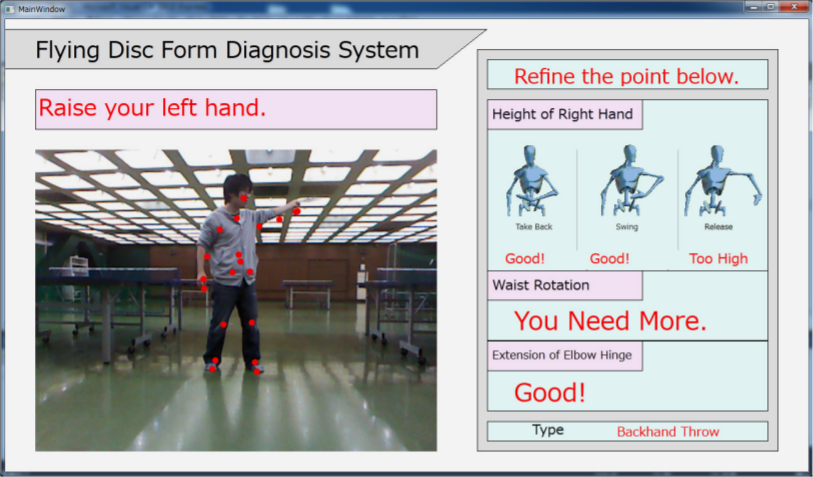
\includegraphics[width=\textwidth]{pictures/flying_disc_TEL.png}
    \caption[Système d'apprentissage du lancer de disque \parencite{Yamaoka2013FoF}]{Le système développé par Yamaoka \textit{et al.} pour l'apprentissage du lancer de disque. Les conseils sont donnés sur plusieurs caractéristiques du geste en même temps \parencite{Yamaoka2013FoF}.}
    \label{fig:flying_disc_TEL}
\end{figure}

Comme présenté précedemment, les travaux de Morel proposent l'extraction de descripteurs du mouvement dans le cadre de l'analyse de la performance sportive \parencite{Morel2017Mts}. Après un recalage spatial (à l'aide d'une transformation linéaire) et temporel (à l'aide de l'algorithme de la \textit{DTW}), les différences spatiales et temporelles entre le geste de l'apprenant et celui de l'expert sont données en calculant d'une part l'alignement spatial d'un membre par rapport au membre de référence, et d'autre part la différence entre les chemins de déformations induits par les alignements des membres de l'apprenant et de l'expert. Ces erreurs sont ensuite traduites en indications pour la position des membres au cours du mouvement.


Le système de Makio \textit{et al.} propose une autre stratégie en se basant sur la trajectoire et la vitesse du poignet lors d'un service au tennis, afin de mettre en lumière les différences entre les gestes des experts et ceux des débutants \parencite{Makio2007DoS}. L'analyse se base sur une extraction des règles d'associations entre les différentes parties du corps, à partir desquelles sont extraits des motifs fréquents. La distance entre ces motifs est calculée à l'aide d'une distance euclidienne. Bien que cette analyse permette de mettre en évidence les différences entre les gestes de l'expert et ceux de l'apprenant, et propose également une visualisation des trajectoires de l'expert et de l'apprenant, aucun conseil n'est ensuite donné par le système.

Dans le domaine de la danse, le système proposé par Maes \textit{et al.} permet d'apprendre le geste en trois étapes : la démonstration, l'apprentissage et l'évaluation ludifiée \parencite{Maes2012DtM}. L'étape de démonstration permet à l'expert de s'enregistrer, tout en configurant plusieurs options telles que la musique, le tempo, le nombre de pas par figure de danse, le nombre d'entraînements requis, \textit{etc.} L'apprentissage se base sur la reproduction des pas effectués par le modèle de l'expert, autant sur l'aspect spatial que temporel, accompagné par les schémas des différents déplacements et rotations à effectuer. Dès cette étape, la corrélation entre le modèle de l'expert et la performance de l'apprenant est calculée, afin de fournir un premier retour sur la performance de ce dernier, à l'aide du coefficient de corrélation croisée de Pearson, calculé sur les données de mouvement de l'expert. Enfin, la partie d'évaluation propose à l'apprenant de danser et effectue une comparaison, toujours selon le même critère, des différents mouvements constituant la danse, permettant ainsi l'évaluation sous la forme d'un score à maximiser. Cette méthode passe cependant outre les spécificités de chaque partie du corps et ne propose qu'une évaluation globale du mouvement, ce qui résulte en une perte d'informations, notamment au niveau des défauts ponctuels du geste.

Toujours dans le domaine de la danse, Kyan \textit{et al.} ont développé un système utilisant la réalité virtuelle afin de faciliter l'évaluation de la performance de l'apprenant \parencite{Kyan2015ABD}. En utilisant un unique descripteur, à l'aide d'une projection dans un espace sphérique des mouvements de danse, le mouvement est décomposé en plusieurs parties. Chacune de ces parties est ensuite comparée à une base de données de composants gestuels d'expert réalisés au préalable. Cette décomposition permet d'estimer quel mouvement était en train d'être réalisé par l'apprenant. Une fois que le mouvement est reconnu, une comparaison entre des descripteurs angulaires extraits permet de donner un score pour chaque partie du mouvement de danse. Ce score est calculé en fonction de la distance euclidienne entre les signaux de l'apprenant et de l'expert, après alignement temporel à l'aide de l'algorithme du DTW. Une autre partie de ce système permet également de superposer le modèle de l'apprenant à celui de l'expert, afin de corriger précisément la position de chaque partie du corps concernée. L'évaluation conduite montre que le mouvement est correctement segmenté par le système ; cependant, la visualisation des mouvements ne permet qu'une faible amélioration de la performance de l'apprenant. De plus, aucun alignement morphologique, spatial ni temporel n'est effectué.

\begin{figure}
    \centering
    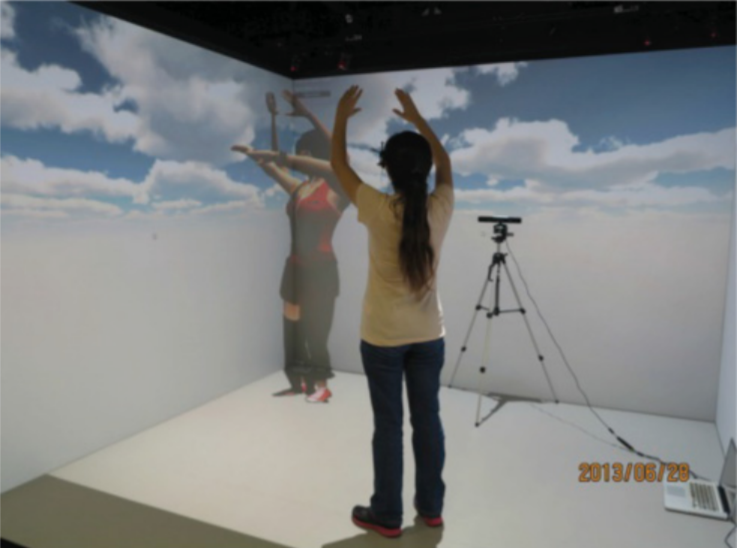
\includegraphics[width=\textwidth]{pictures/dance_cave_TEL.png}
    \caption[Système d'apprentissage de mouvement utilisant un CAVE pour la captation et la comparaison \parencite{Kyan2015ABD}]{Le système développé par Kyan \textit{et al.} fait usage de la réalité virtuelle dans un système CAVE afin de proposer soit une observation côte à côte des mouvements de l'expert et de l'apprenant, soit superposée (cas de l'image) \parencite{Kyan2015ABD}.}
    \label{fig:dance_cave_TEL}
\end{figure}

Toujours dans le domaine des arts, l'analyse des efforts réalisés par les joueurs de violon est le sujet d'étude de Rasamimanana et Bevilacqua\parencite{Rasamimanana2008EbA}. À partir d'informations cinématiques provenant du geste de la personne, telles que : la vitesse, le tremblement (\textit{jerk}) et l'impulsion (du mouvement), il est possible de déterminer quel a été le mode de jeu utilisé par la personne réalisant le geste : \textit{détaché} ou \textit{martelé}.

Les systèmes calculant des indicateurs à partir du geste de l'apprenant permettent, dans une certaine mesure, de s'affranchir de la présence de l'expert pour l'évaluation et la restitution des conseils à l'apprenant. Leur objectif est souvent de proposer une évaluation de manière automatique, sans nécessiter l'intervention d'un expert pour interpréter les données. La connaissance experte doit être intégrée \textit{a priori}, dès la phase de conception. Dans ce contexte, la généricité des descripteurs extraits n'est pas assurée si elle n'est pas considéré dès la conception du système, et le système n'est souvent pas réutilisable dans des contextes différents. De plus, les retours données prennent le plus souvent la forme d'un score à maximiser (indiquant généralement la proximité des données de l'apprenant à celles de l'expert), qui, bien que facilement interprétable en terme de qualité du geste effectué, ne permet pas systématiquement de fournir des indications quant aux améliorations à apporter au geste.


\section{Analyse par détection d'une séquence ordonnée d'actions}
Dans les systèmes d'apprentissage du geste, l'analyse peut se focaliser sur la suite d'actions à réaliser afin d'atteindre l'objectif. Dans ce cas, le geste est décomposé en unités considérées comme élémentaires par le système afin de représenter chaque action. La granularité des unités élémentaires est dépendante du système considéré. Ainsi, il est possible de comparer cette suite de mouvements de manière ordonnée à l'enchainement attendu par l'expert.

%Dans ces travaux, on retrouve les études qui s'intéressent à la manipulation d'objets. Ainsi, dans les travaux de Toussaint, à partir de traces hétérogènes (manipulation d'un objet simulant un trocart, mais également position du regard) et d'un ensemble de séquences à réaliser prédéfinies par un expert, l'objectif est de permettre à la fois l'évaluation des connaissances de l'apprenant et de lui donner des retours en fonction du type de défaut présent au sein de la procédure. Le mouvement à reproduire est divisé en phases, chaque phase comprenant une suite de plusieurs actions. La finalité du système est de comparer la séquence d'actions (appelées « perceptivo-gestuelle », car combinant des données relatives au regard de l'apprenant et du mouvement de l'objet) aux séquences pré-définies par les experts \parencite{BMT_2015}. Bien qu'il existe un ordre précis pour les phases, déterminé à l'avance par l'expert, le système ne contraint pas l'ordre des phases de résolution de l'opération, c'est-à-dire que l'apprenant peut librement passer d'une phase à une autre au cours de l'opération. Cependant, ces changements de phases sont analysés par le système, et interprétés comme étant une erreur dans l'opération qui est constatée par l'apprenant. Le nombre de retours en arrière est corrélé à une faible maîtrise des connaissances à appliquer. Ainsi, il est possible d'évaluer à la fois si les gestes sont effectués dans le bon ordre, mais également si l'ordre des phases est correct. Cependant, le ou les gestes menant à la réalisation des actions ne sont pas directement évalués, l'analyse se focalisant sur la détection d'une suite ordonnée d'actions.

Mahdi \textit{et al.} ont développé un environnement virtuel permettant à n'importe-quel enseignant de définir lui-même ses scénarios d'apprentissage à partir de scènes virtuelles pré-existantes \parencite{Mahdi2019TaE}. L'objectif est de permettre de lier la description du scénario pédagogique aux activités de l'apprenant au sein de l'environnement virtuel. Chaque activité peut être divisée en une séquence d'actions, qui elles-mêmes peuvent être divisées en séquences de comportements élémentaires, appelées " Primitives Virtuelles de Comportement " : (i) observation du monde virtuel, (ii) déplacement dans le monde virtuel, (iii) interaction avec le monde virtuel et (iv) communication avec d'autres personnes ou avec l'application. Les activités sont réalisées par l'apprenant à l'aide d'objets d'intérêt auxquels ont été associés des propriétés techniques (position, forme, couleur, \textit{etc.}) ou pédagogiques (utiliser l'objet, verser, le bouger, \textit{etc.}). L'éditeur de scénario permet ainsi à l'expert de définir une suite d'activités lors de la conception du scénario. Les premiers tests à l'aide d'enseignants ont montrés que l'éditeur leur était utile, et permettait de générer des scénarios de manière aisée.

Les travaux de Delest \textit{et al.} ont mené à la création d'un système où l'expert peut lui-même proposer un parcours, personnalisable à l'aide de points de contrôle (\textit{checkpoints}), représentés sous la forme d'objets 3D simples (e.g. sphère, parallélépipède rectangle) à passer dans un ordre précis \parencite{Delest2019MaE} (Fig. \ref{fig:Delest_system}). Dans ce système, l'expert doit déterminer à l'avance si le parcours concerne le corps de l'apprenant (analyse de la démarche, par exemple) ou un objet présent au sein de la scène. Une fois l'objet d'intérêt choisi, l'expert place ensuite un point de contrôle de départ, possiblement des points de contrôles intermédiaires puis un point de contrôle d'arrivé. Il est possible de modifier la taille et la forme de ces points de contrôles, permettant ainsi de les adapter aux différents objets manipulables (Fig. \ref{fig:Delest_system} au milieu). L'expert doit ensuite réaliser le mouvement lui-même, afin de disposer d'un mouvement de référence (mouvement cible). Le mouvement est considéré comme validé lorsque l'objet ou la personne a franchi (c'est-à-dire qu'il y a collision entre le point de contrôle et l'objet ou la personne) tous les points de contrôle dans l'ordre. Le mouvement est ensuite segmenté en fonction des points de contrôle. Chaque mouvement est ensuite comparé au mouvement de référence réalisé par l'expert, selon plusieurs métriques : de manière globale à l'aide de l'algorithme du DTW, mais également à l'aide d'indicateurs cinématiques, tels que la vitesse, la saccade du mouvement (\textit{jerk}), \textit{etc.} (Fig. \ref{fig:Delest_system} à droite).

\begin{figure}
    \centering
    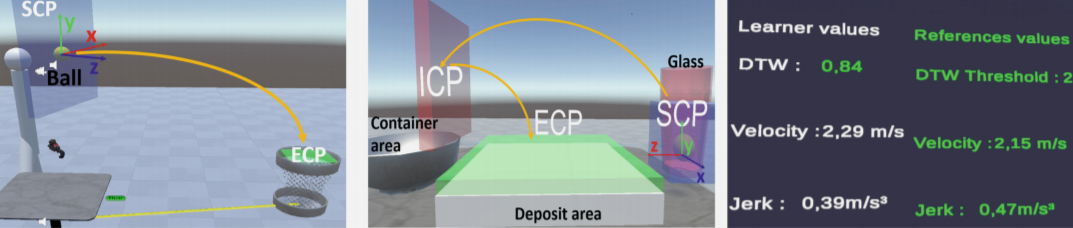
\includegraphics[width=\textwidth]{pictures/Delest_system.png}
    \caption[EVAH permettant de générer des parcours à suivre pour un objet ou l'apprenant \parencite{Delest2019MaE}]{Le système proposé par Delest \textit{et al.} permet à l'expert de générer un parcours à suivre, soit pour la personne, soit pour un objet, dans un ordre prédéfini, et propose l'affichage de plusieurs métriques permettant de comparer le geste de l'apprenant à celui de l'expert \parencite{Delest2019MaE}.}
    \label{fig:Delest_system}
\end{figure}

Dans ces systèmes, l'évaluation du geste est principalement centrée sur l'ordre dans lequel est réalisé un ensemble d'unités élémentaires, plutôt que sur l'évaluation en elle-même du geste sous-jacent à ces actions ou unités. Ainsi, les caractéristiques du geste ne sont pas systématiquement analysées (excepté pour \parencite{Delest2019MaE}). Lors de la manipulation d'objets, c'est l'état de l'objet à des moments clés du mouvement qui va être considéré. Dans ce cas, on considère que le geste qui a mené à l'état cible est correct, sans l'analyser en lui-même.

Ces systèmes fonctionnent par décomposition et analyse des unités élémentaires composant le geste initial. La nature de ces unités élémentaires (durée, granularité de la décomposition, \textit{etc.}) peut varier d'un système à l'autre. La finalité de cette décomposition est de comparer l'enchainement d'unités élémentaires à l'enchainement attendu par l'expert. Cela implique de disposer d'un modèle de connaissance du geste à effectuer, et son intégration se fait souvent dès la conception du système, ne permettant pas d'assurer sa généricité. Cependant, des systèmes tels que ceux développés par Delest \textit{et al.} \parencite{Delest2019MaE} et Mahdi \textit{et al.} \parencite{Mahdi2019TaE}, conçus afin être génériques au regard du geste à accomplir, permettent une ré-intégration de la connaissance experte aisée à l'aide d'un éditeur de scénarios pédagogiques intégrés au système. L'apprentissage se focalise néanmoins sur la suite d'action à réaliser, leur enchainement et la manipulation d'un objet, mais pas sur les gestes qui permettent d'arriver aux états ou à la succession de postures désirés.


\section{Analyse fondée sur des techniques d'apprentissage automatique}
Il est également possible d'utiliser des algorithmes d'apprentissage automatique afin d'analyser automatiquement le geste. Dans ce cas, les descripteurs extraits sont le plus souvent choisis en amont du processus d'analyse, puis utilisés dans un algorithme d'apprentissage automatique afin d'observer la similitude entre le mouvement et ceux présents au sein d'une base de données.

Par exemple, les travaux de Pirsiavash \textit{et al.} proposent une approche sur l'évaluation de geste sans \textit{a priori} sur le mouvement en lui-même \parencite{Pirsiavash2014AQA}. Les données sont extraites à partir de vidéos, et sont constituées de descripteurs variés, tels que des gradients de pixels, des vitesses et des trajectoires, ainsi que des postures successives réalisées par les sportifs. Cette étude se base sur les performances d'athlètes olympiques dans deux sports différents, la patinage artistique et le plongeon. Les données extraites sont ensuite associées à un score donné par des experts ; dans ce cas, il s'agit de scores donnés par les juges olympiques. L'étude montre que les juges donnent la même note dans 96\% des cas, ce qui suggère qu'il existe un socle de règles communes permettant l'évaluation. Les couples mouvements / score sont ensuite utilisés en entrée d'un SVM. L'algorithme a permis d'extraire les moments les plus déterminants dans l'attribution du score par les juges. Les scores donnés par l'algorithme sont comparés à ceux données par l'expert, à l'aide de la corrélation de Spearman. Les valeurs de ce coefficient montre que les scores donnés sont encore assez éloignés de ceux des experts. L'analyse permet néanmoins de mettre en évidence une évaluation de la qualité du geste supérieure à celle d'un non-expert du domaine.

Patrona \textit{et al.} utilisent des algorithmes de logique floue (\textit{fuzzy logic}) afin de proposer une segmentation, une reconnaissance et une évaluation de gestes \parencite{Patrona2018MaA}. Il n'y a pas d'\textit{a priori} sur les gestes pouvant être traités par le système. Dans cette études, les gestes considérés sont variés, tous pris au sein de bases de données : \textit{swing} au golf, taper dans ses mains, s'asseoir, lancer, service au tennis, \textit{etc.} Des descripteurs cinématiques sont extraits du mouvement, puis utilisés par des classifieurs binaires, chacun entrainé à reconnaître un mouvement spécifique. Une fois le mouvement reconnu par le système, la phase d'évaluation s'effectue entre le mouvement de l'apprenant et les mouvements cibles contenus dans la base de données de mouvements. Plusieurs étapes sont ensuite réalisées (Fig. \ref{fig:Patrona_motion_evaluation}) : alignement temporel des mouvements (apprenant et cible) à l'aide d'un algorithme de DTW multivarié, normalisation de la longueur des membres afin d'éviter les différences morphologiques, alignement spatial des mouvements à l'aide de la différence de rotation du corps calculée à partir de la position des épaules et du torse, puis utilisation des différences de positions et de vitesses entre les deux mouvements afin de proposer un retour à l'apprenant. Ces retours sont donnés sous la forme d'un score de similarité entre les mouvements (calculé à l'aide de l'algorithme du \textit{DTW}), mais également les parties du corps et les articulations les plus éloignées de celles de l'expert, au regard des descripteurs utilisés (positions et vitesses). Un exemple de retour donné par le système est le suivant :

\vspace{0.5cm}« The highest \textit{POSITION} error is detected at \textbf{Left Wrist}, at the \textbf{Latest} temporal phase (frame 26) of the movement. Please, position your \textbf{Left Wrist Left} and \textbf{Down}, at this time instance. »

Ainsi, le retour donné ne considère que des localités temporelles et spatiale, sans tenir compte du geste dans sa globalité. Il peut être difficile pour un apprenant, à partir de ces seules indications, d'être en mesure de modifier les parties du geste suggérées par le système, afin de respecter les conseils donnés par ce dernier, tout en gardant un geste acceptable dans sa globalité.

\begin{figure}
    \centering
    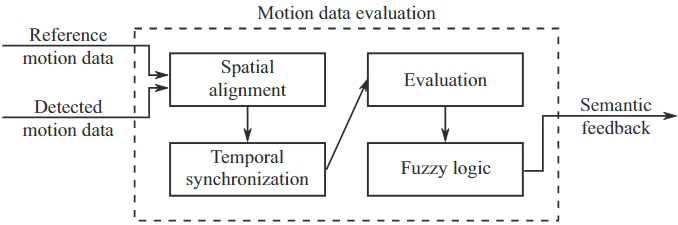
\includegraphics[width=\textwidth]{pictures/Patrona_motion_evaluation.png}
    \caption[Étapes de normalisation et d'analyse automatique du mouvement \parencite{Patrona2018MaA}]{La suite d'étapes utilisée par Patrona \textit{et al.} permet de corriger les différences spatiales et temporelles entre les mouvements de l'expert et de l'apprenant, afin de proposer une évaluation du geste en fonction des descripteurs extraits \parencite{Patrona2018MaA}.}
    \label{fig:Patrona_motion_evaluation}
\end{figure}

Dans ces travaux, la contribution de l'expert se situe en amont, lors de la formalisation de ses besoins d'observations en descripteurs calculables à partir du mouvement, voire des conseils à donner. Cependant, les données obtenues en sortie de ces systèmes doivent parfois être analysées et traduites en retour intelligible à l'apprenant par un expert. Dans tous les cas, l'expert n'intervient pas pendant le processus d'apprentissage humain. Lorsque le retour est donné par le système, les informations fournies concernent les propriétés extraites du geste : différence de positions, vitesses, \textit{etc.} Ces informations sont difficilement observables pour un apprenant sans visualisation externe, mais également dans le cas où l'apprenant ne possède pas les connaissances scientifiques requises pour être en mesure de modifier son geste pour prendre en compte les retours du système.

\section{Bilan des systèmes existants et positionnement}
Cette section présente les modalités d'usage des différentes systèmes présentés auparavant, tout en mettant en lumière leurs avantages et inconvénients par rapport à la place donnée à l'apprenant, ainsi qu'à l'enseignant, en leur sein.


Les travaux où l'analyse des gestes est réalisée par un humain sont ceux où les utilisateurs finaux (experts dans le cas d'un sytème d'assistance à l'analyse et l'évaluation du geste, ou apprenants) ont une place importante. Les systèmes dédiées à l'analyse médicale (rééducation ou suivi de maladie) nécessitent très souvent de combiner les retours proposés par le système (squelette 3D de démarche, descripteurs spécifiques extraits des parties du corps lors d'un mouvement, \textit{etc.}) au savoir de l'expert, afin de proposer un diagnostic adéquat. Dans ces cas, le système n'a pas pour objectif d'être utilisé par le patient en autonomie, car les informations fournies par le système nécessitent de disposer de la connaissance scientifique permettant d'en tirer des conclusions, et sont ainsi destinées à un expert. L'apprentissage de procédures chirurgicales au travers d'EIAH dédiés permet de proposer des entrainements sur des simulations d'opérations réelles. Dans ce cas, la connaissance experte est parfois directement intégrée au système \textit{a priori} (ordre des différents mouvement à réaliser, état successifs de l'objet à atteindre, temps total de l'opération, \textit{etc.}), ce qui permet de calculer des indicateurs précis sur le geste, correspondants aux besoins d'observation et d'analyse de l'expert. L'apprentissage du sport nécessite également très souvent un expert afin de proposer des retours compréhensibles sur le geste et exploitables par un apprenant afin de modifier son geste. Le système proposé par Burns \textit{et al.} ne propose aucun retour en lui-même, et ne sert que de support à la visualisation des mouvements de l'expert (soit sous forme de vidéo, soit sous la forme d'un squelette 3D représentant l'expert en train d'effectuer le mouvement, dans un contexte de réalité virtuelle en immersion dans un dojo virtuel). L'évaluation du geste de l'apprenant s'effectue à la fin de l'apprentissage d'un geste par l'expert, en visualisant la vidéo de l'apprenant en train d'effectuer le mouvement. L'environnement virtuel de Kora \textit{et al.}, à l'inverse des systèmes vus précédemment, ne fait intervenir l'expert que dans la phase d'enregistrement du geste cible. Le système est utilisé en autonomie totale par l'apprenant, et l'objectif est d'ajuster le geste de façon à se rapprocher le plus possible visuellement du geste cible de l'expert. Le système ne fournissant aucun conseil ni aucune métrique (indicateurs, score), l'ajustement du geste peut être difficile pour un apprenant non-expert. Enfin, le système de Yoshinaga et Soga utilise plusieurs données expertes différentes afin de proposer une comparaison du geste de l'apprenant à celui des experts les plus proches de l'apprenant au sens morphologique \parencite{Yoshinaga2015Doa}. Dans celui-ci, les experts enregistrent non seulement les mouvements cibles, mais peuvent également utiliser le système afin d'analyser le geste de l'apprenant et pour proposer un retour visuel des changements à effectuer sur le geste, en fonction des parties du corps concernées. Le système peut également être utilisé en autonomie par l'apprenant, qui ne dispose alors que de la visualisation de la superposition du mouvement cible choisi avec le sien.

Dans les systèmes où l'analyse est réalisée par un humain, l'implication de l'expert dans la conception dépend souvent de la nécessité ou non de disposer de matériels ou environnements spécifiques à la tâche considérée. Les systèmes proposant de calculer des métriques, à partir du mouvement de l'apprenant, interprétables par les experts nécessitent d'impliquer ce dernier dans le processus de conception afin d'être en mesure de satisfaire ses besoins d'observation. Les valeurs ainsi calculées à partir du geste de l'apprenant ne sont, en général, pas réutilisables dans d'autres contextes applicatifs. De plus, dans les systèmes dédiés à l'apprentissage de procédures chirurgicales, la réutilisabilité est compromise à cause de l'utilisation de matériels spécifiques (bras haptiques, par exemple). À l'inverse, les systèmes ne proposant qu'une visualisation du mouvement (soit de l'expert pendant l'apprentissage de l'apprenant, soit de l'apprenant lors de la phase d'évaluation de l'expert) sont en général très génériques et ne nécessitent ainsi pas d'intégrer l'expert dans le processus de conception, mais ne proposent en général aucune analyse sur le mouvement de l'apprenant, et n'assistent donc l'expert dans sa tâche d'évaluation que de manière marginale.

L'extraction de descripteurs à partir du geste de l'apprenant permet de fournir un ensemble de valeurs afin de l'assister dans son évaluation. Ainsi, le système de suivi de patients atteints de la maladie de Parkison proposé par Wang \textit{et al.} nécessite de faire réaliser au patient quelques mouvements types (marcher, s'asseoir, se lever), permettant ensuite de calculer des descripteurs relatifs au déplacement du patient. Les experts médicaux peuvent ensuite utiliser ces indications afin de juger de la progression du système. Il a également été pensé de manière à permettre au patient de réaliser les gestes requis à distance, afin de limiter le déplacement de ce dernier. La place du patient au sein du système se limite à effectuer les gestes demandés par l'expert ou le système. Le système de simulation d'insertion de sonde naso-gastrique développé par Choi \textit{et al.} permet de calculer la force appliquée par l'apprenant, mais également de simuler les butées contre les parois d'un modèle 3D mis à jour en temps réel \parencite{Choi2015103}. Les indicateurs extraits sont relatifs à la procédure (durée de l'opération, nombre de butées, force maximale appliquée, \textit{etc.}), et bien que leur restitution soit proposée par le système, leur analyse nécessite un expert afin d'être capable d'en tirer des conclusions sur le déroulement de l'opération, et sur les conseils à donner afin d'améliorer le geste de l'apprenant. De par la spécificité du matériel utilisé et des indicateurs calculés, le système n'est pas réutilisable dans d'autres contextes.
Les outils d'analyse automatique permettent d'évaluer le geste suivant des descripteurs géométriques, cinématiques, dynamiques et de les comparer. Cependant, des connaissances scientifiques solides sont nécessaires, tant pour l'enseignant que pour l'apprenant afin de pouvoir les interpréter. Les indicateurs utilisés peuvent parfois concerner l'objet manipulé, plutôt que le mouvement en lui-même. Dans le cas de l'EIAH développé par Pham \textit{et al.}, la trajectoire de l'outil de l'apprenant est comparée à celle de l'outil manipulé par l'expert, et cette comparaison fourni un score de similitude entre les gestes \parencite{Pham2010Tdg}. Bien qu'étant facile à interpréter pour un non-expert (la maximisation de ce score étant l'objectif), aucune indication n'est fournie sur les parties du geste à modifier afin de se rapprocher des positions de l'objet ciblées. Le même principe est utilisé par Maes \textit{et al.} dans leur système dédié à l'apprentissage de la danse, en segmentant cette fois le mouvement en plusieurs parties et en assignant un score (correspondant à la similitude des mouvements de l'apprenant par rapport à ceux de l'expert) à maximiser pour chaque partie du mouvement \parencite{Maes2012DtM}. Il n'y a toujours aucun retour proposé à l'apprenant afin d'améliorer son geste. Le système d'apprentissage de la danse proposé par Kyan \textit{et al.} utilise les mêmes concepts, mais propose en plus de cela une superposition du mouvement de l'apprenant avec celui de l'expert, afin de corriger la position de chaque partie du corps \parencite{Kyan2015ABD}. Le système proposé par Yamaoka \textit{et al.} évalue le geste du lancer de disque d'un apprenant en comparant les positions relatives des articulations entre elles à différents moment du geste. Ici, la connaissance experte est intégrée dès la conception de l'environnement, et la réutilisabilité du système dans un autre contexte nécessite une re-conception du système. De plus, les retours fournis par le système le sont en temps réel, et il n'est pas possible de rejouer le mouvement, ce qui rend plus difficile la correction et l'apprentissage du geste pour l'apprenant. L'objectif du système développé par Makio \textit{et al.} est de mettre en lumière les différences entre les gestes des apprenants et des experts, sans pour autant fournir des indications ou des retours sur les corrections à effectuer. Ainsi, l'expert et l'apprenant n'ont qu'un rôle minime au sein de la conception, et la phase de restitution en propose qu'une visualisation graphique de ces différences.

Les systèmes se basant sur le calcul d'indicateurs à partir du geste de l'apprenant permettent de s'affranchir dans une certaine mesure de la présence d'un expert pendant l'apprentissage. En effet, ils sont généralement conçus dans l'optique de proposer une évaluation du geste de l'apprenant, souvent en le comparant aux données de l'expert intégrées au préalable lors de la conception du système. Les inconvénients de ces systèmes sont le côté peu explicite des retours ainsi donnés, se limitant souvent à un simple score, et la faible réutilisabilité dans d'autres contextes, due à la nécessiter d'intégrer la connaissance experte dès la phase de conception du système.

Les outils d'analyse automatique du mouvement sont souvent conçus et développés dans l'objectif d'aider et d'assister l'expert et l'apprenant. En conséquence, la formalisation de la connaissance de l'utilisateur et de ses besoins d'observation est nécessaire, mais difficile à opérationnaliser. Le développement de ce type de systèmes a pour objectif de répondre aux défis d'adaptation au contexte d'apprentissage constitué du profil d'utilisateur (apprenant ou enseignant), du domaine d'application et de la tâche à apprendre. La généricité potentielle du système ainsi développé peut grandement varier suivant le contexte.

Les systèmes s'intéressant à la détection d'une suite d'action ordonnées au sein d'un mouvement vont dans un premier temps segmenter le mouvement en unités élémentaires, pour ensuite proposer une représentation de chacune de ces unités comparable à l'enchainement attendu par l'expert. Ces travaux nécessitent ainsi l'intégration de la connaissance experte dès la conception du système, et fait qu'ils ne sont habituellement pas génériques. Il est cependant intéressant de noter que les systèmes développés par \parencite{Mahdi2019TaE} et \parencite{Delest2019MaE} ont pris en compte la réutilisabilité du système dès la conception, et proposent ainsi des éditeurs de scénarios pédagogiques utilisables par des non-expert de la réalité virtuelle.

Enfin, les systèmes faisant usage d'apprentissage supervisé afin d'observer la similitude des mouvements de l'apprenant à ceux de l'expert nécessitent également l'intégration de la connaissance experte \textit{a priori}, afin d'utiliser l'ensemble de caractéristiques des gestes les plus pertinents afin d'obtenir la meilleure séparation possible. Le système d'évaluation de gestes développé par Patrona \textit{et al.}, bien que permettant de segmenter des gestes et de les reconnaitre sans a priori sur ces derniers \parencite{Patrona2018MaA}, nécessite une base de données de geste de comparaison suffisamment importante afin de couvrir les différents gestes possibles à reconnaitre.

Ce chapitre a présenté plusieurs techniques d'analyse du mouvement, classées en quatre catégories : (i) l'évaluation par observation, (ii) l'évaluation par analyse d'indicateurs calculables  et (iii) l'évaluation d'une séquence ordonnée d'actions (iv) l'évaluation utilisant des techniques d'apprentissage automatique. Cette étude a aussi montré l'importance de la prise en compte des connaissances et besoins d'observation de l'expert dans le processus d'observation et d'analyse, ce qui implique de placer l'expert dans le processus de conception du système informatique dédié à l'apprentissage humain.

L'analyse peut se faire à partir du geste en lui-même ou d'un découpage du geste en unités élémentaires \parencite{Despinoy2016UTS} \parencite{Yamaoka2013FoF} \parencite{Pirsiavash2014AQA}. Les mouvements sont souvent modélisés sous la forme d'un ensemble d'informations cinématiques, telles que les positions, les orientations, les vitesses, les trajectoires, la courbure du mouvement, etc. L'utilisation de tels descripteurs permet d'obtenir des informations précises à traiter. Des descripteurs fournissant des informations globales sur le geste, bien que plus facilement compréhensibles et utilisables pour l'analyse pour un humain non-expert, ne permettent pas de systématiquement mettre en évidence les différences subtiles qui permettent de juger de la qualité d'un geste.

L'apprentissage par observation et imitation est naturelle pour l'humain. Cependant, cette méthode se heurte aux capacités de perception et de connaissances de l'usager qui ne percevra pas nécessairement les propriétés du geste rendant ce dernier comme acceptable. En outre, l'analyse de toutes les caractéristiques d'un geste ainsi que leurs propriétés est difficile, tant ils dépendent des caractéristiques de la situation d'apprentissage qui demeure très contextuel. L'utilisation d'outils informatiques proposant des indicateurs quant à la performance ou la qualité du geste permet ainsi à l'expert de proposer un retour plus pertinent mais nécessitent des connaissances scientifiques solides pour être interprétés; ainsi qu'une phase de formalisation des besoins d'observation en amont.

En effet, dans le cas où les descripteurs utilisés sont extraits par un processus automatique, l'analyse en elle-même est souvent réalisée par un humain. De plus, il est difficile de proposer un retour pédagogique pertinent à l'apprenant à partir d'un processus entièrement automatisé. Dans ce cas, il faut disposer à minima d'un modèle d'expertise pédagogique, et d'un modèle de l'apprenant. Au-delà de la difficulté propre à l'extraction de descripteurs pertinents dans un cadre donné, il faut également être en mesure de fournir des indications suffisamment explicites afin que même une personne non-experte du domaine puisse être en mesure de s'auto-corriger. Bien que l'injection de la connaissance experte permet de formaliser et, par exemple, d'intégrer en amont un ensemble de conseils, ce type de systèmes est souvent réalisé de façon « \textit{ad hoc} », contextuel au domaine voire à la tâche à apprendre et peut être limité dans le cas de problèmes non-définis à l'avance.

En outre, l'outil utilisé et la connaissance experte ne se rejoignent pas forcément. Par exemple, le système de \parencite{Kyan2015ABD} propose un score pour évaluer chaque sous-partie du geste de danse, mais c'est à l'enseignant de donner les indications et corrections nécessaires afin d'améliorer le geste. Ainsi, l'outil informatique propose une pré-évaluation du geste, utilisable ou non par l'expert. L'analyse d'un geste étant matière à une certaine part de subjectivité de la part de l'expert, une étude purement automatique peut parfois ne pas être en accord avec l'avis de l'expert.

L'association des compétences de l'expert tout au long du processus d'apprentissage et d'évaluation avec l'aide possible apportée par un outil informatique est une approche qui semble être peu explorée. Un système permettant à la fois d'évaluer le geste, mais également de proposer un ensemble d'indicateurs visuels pourrait aider l'expert dans sa tâche d'évaluation lorsque l'observation n'est pas aisée. Il faut cependant qu'un tel système puisse disposer de la connaissance experte en amont, afin de pouvoir formaliser les différentes modalités du geste à analyser, et également qu'il soit en mesure de proposer des visualisations pertinentes et compréhensibles à partir des descripteurs calculés.

Le prochaine chapitre présente un système d'aide à l'observation, l'analyse et l'évaluation de gestes. Ce système est développé de manière à minimiser les travaux de réingénierie en cas de changement du geste cible à apprendre et des besoins d'observation.

\include{chapters/plateforme_MLA}

\part{Contributions}

\chapter{Traitement des données de mouvement}\label{chap:traitement_donnees}
Les chapitres précédents montrent que la capture de mouvement peu prendre place dans de nombreux contextes. Les besoins en termes d'observation et d'analyse peuvent varier grandement en fonction du domaine ciblé. Il est nécessaire de choisir un système de capture adapté, au regard des besoins d'observation mais également des contraintes de place, de coûts et de temps d'acquisition. De plus, il est nécessaire de disposer d'un ensemble d'outils logiciels afin de pouvoir extraire, à partir des données, des informations utiles pour l'apprentissage d'un geste. Ces informations peuvent être de plusieurs natures : il est possible de proposer une comparaison précise entre les données de l'expert et celles de l'apprenant (\textit{e.g.} " la position du coude est 4cm trop bas au moment $T$ du mouvement "), bien que cette méthode soit soumise aux problèmes de différences de morphologie, d'alignement temporel des séquences de mouvements, etc. Il est également possible de fournir des indications de plus haut-niveau (\textit{e.g.} " La vitesse lors du lancer doit être plus élevée "). Dans tous les cas, ces informations peuvent soit être utilisées telles quelles par l'apprenant, soit être utilisées par l'expert afin d'affiner son jugement du geste. Certaines conditions font qu'il n'est pas toujours possible pour un expert d'observer toutes les modalités importantes du geste pendant sa réalisation (trop de parties du corps à regarder, difficile de voir certaines parties du corps lors de l'exécution du geste, \textit{etc.}). La proposition d'outils d'aide à la décision permet ainsi d'aider l'expert dans sa tâche d'évaluation et de remédiation.

Ce chapitre présente l'artefact informatique développé pour répondre aux besoins de la thèse, nommé \textbf{Motion Learning Analytics} (\textbf{MLA}), ainsi que les différentes étapes du processus associé, du traitement des données de mouvements jusqu'à l'aide proposée à l'expert.

\section{Motion Learning Analytics (MLA)}
Dans cette partie, nous présentons la plateforme Motion Learning Analytics (MLA), créée pour répondre à nos besoins d'extraction et d'analyse de données de mouvement.

L'objectif de \textit{MLA} est de proposer un ensemble d'outils permettant d'extraire des informations permettant d'analyser un geste à partir de données de mouvement bas-niveaux, afin de pouvoir être utilisées par un humain \textit{a posteriori} afin d'aider au jugement de la qualité d'un geste en fonction du domaine applicatif. Il existe d'ores et déjà de nombreux systèmes d'analyse du mouvement. Ces systèmes ont déjà fait l'objet d'analyses. L'une d'entre elle propose une classification partielle selon l'objectif de ces systèmes \parencite{Wang2003Rdi} : la détection d'humains, le suivi (\textit{tracking}) d'humains et la reconnaissance d'activité. Bien que ces domaines soient larges et très explorés dans la littérature \parencite{Yang2011Raa} \parencite{Aggarwal2014Har}, ils concernent plutôt la segmentation et  l'extraction de mouvements au sein de différents types de données, tels que la vidéo ou des enregistrements partiels à l'aide de capteurs de parties du corps. De plus, le contexte applicatif est souvent secondaire et ces systèmes sont développés de manière à proposer des méthodes automatique innovantes. A l'inverse, notre approche se concentre sur une application particulière, celle de l'apprentissage du geste, afin de proposer des conseils à un apprenant ou à l'expert qui enseigne ce geste. De plus, l'objectif de notre système est d'être indépendant du geste considéré.

Des systèmes tels que ceux présentés dans le chapitre 2 (\parencite{Ferrari2018MAS}, \parencite{Makio2007DoS}) sont eux conçus pour une tâche ou un domaine en particulier. Le fait d'avoir un domaine ciblé dès le début permet d'orienter le développement et l'analyse afin d'offrir un retour à l'expert le plus exact possible. Le problème se pose dans la réutilisabilité de tels systèmes dans des cas proches : le système n'est pas systématiquement suffisamment modifiable pour être utilisé dans d'autres contextes. L'objectif de MLA est, à terme, de proposer un ensemble d'outils et de descripteurs calculables permettant de couvrir une large gamme de domaines applicatifs, à l'aide de l'injection de la connaissance de l'expert. Elle est divisée en trois parties : le traitement des données de mouvement brutes, de la lecture des fichiers jusqu'à l'extraction des descripteurs, l'analyse des données obtenues à l'aide de techniques d'apprentissage semi-supervisé, et le retour fourni à l'expert et/ou l'apprenant. Ces trois parties sont indépendantes l'une de l'autre, et peuvent être utilisées séparément. Chaque partie est découpée en modules, correspondant à un sous-ensemble de fonctions au sein de l'artefact. Le worklflow complet est présenté dans la figure  \ref{fig:workflow_MLA}.

\begin{figure}[h]
    \centering
    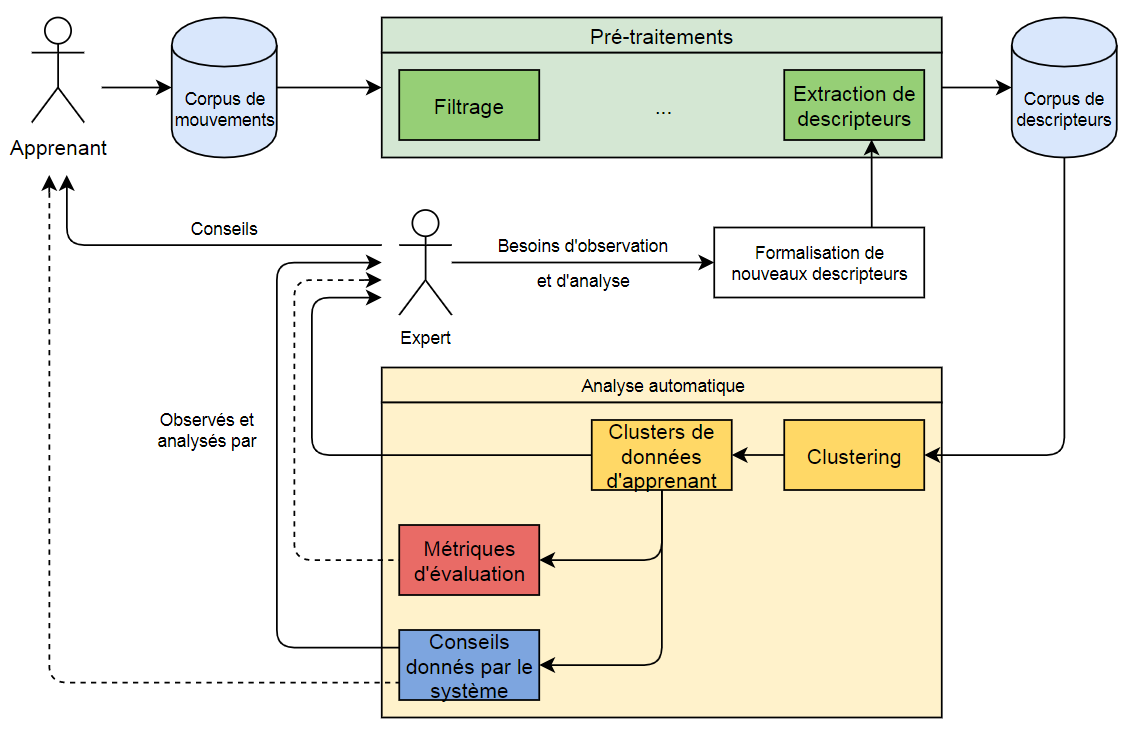
\includegraphics[width=\textwidth]{pictures/MLA_colours.png}
    \caption{Architecture de la plateforme \textit{Motion Learning Analytics} (\textit{MLA}).}
    \label{fig:mla_project}
\end{figure}

\begin{figure}[h]
    \centering
    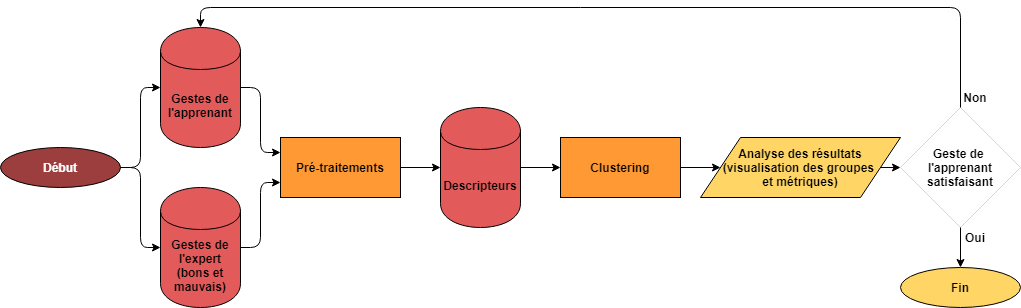
\includegraphics[width=\textwidth]{pictures/workflow_MLA_2.png}
    \caption{Le workflow général de la plateforme \textit{MLA}.}
    \label{fig:workflow_MLA}
\end{figure}

\subsection{Données de mouvement au format BVH}\label{subsec:bvh}
Le système prend en entrée des fichiers au format \textbf{BioVision Hierarchy} (\textbf{BVH}). Ce format de fichier permet de décrire un mouvement, posture par posture. Les fichiers \textbf{BVH} sont constitués d'une partie fournissant des informations sur les articulations composants le squelette, sous forme d'une hiérarchie (Fig. \ref{fig:bvh_hierarchy}), et d'une seconde partie donnant les informations pour chaque articulation sur chaque frame du mouvement (Fig. \ref{fig:bvh_motion}). Plus précisément, chaque articulation peut avoir jusqu'à six informations : trois valeurs relatives à la position dans l'espace, et trois valeurs relatives à l'orientation dans l'espace. Les informations pour chaque articulation sont données relativement à l'articulation parente.

\begin{figure}[h]
    \centering
    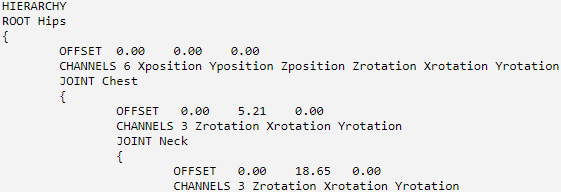
\includegraphics[width=\textwidth]{pictures/bvh_hierarchy.png}
    \caption[Exemple de squelette dans un fichier BVH]{Un exemple de la hiérarchie du squelette au sein d'un fichier BVH (source: \textit{http://research.cs.wisc.edu/graphics/Courses/cs-838-1999/Jeff/BVH.html})}
    \label{fig:bvh_hierarchy}
\end{figure}

\begin{figure}[h]
    \centering
    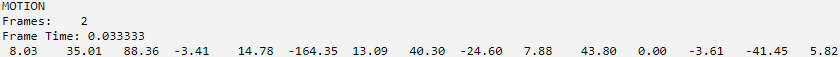
\includegraphics[width=\textwidth]{pictures/bvh_motion.png}
    \caption[Exemple de données de mouvement dans un fichier BVH]{Un exemple de données relatives au mouvement au sein d'un fichier BVH source: \textit{http://research.cs.wisc.edu/graphics/Courses/cs-838-1999/Jeff/BVH.html})}
    \label{fig:bvh_motion}
\end{figure}


\subsection{Pré-traitements des données}
La première partie (pré-traitements) a deux objectifs : (i) filtrer les données si nécessaire, afin d'éliminer les artefacts possibles dûs au matériel de captation, et (ii) extraire des descripteurs à partir du mouvement capturé, afin d'obtenir des informations exploitables. Cette partie est intégralement codée en \textbf{C++11}. Elle partie du système est subdivisée en six modules (Fig. \ref{fig:MLA_architecture}). Le module central de l'architecture contient les classes qui permettent de représenter un mouvement dans son entièreté, à partir d'un fichier \textbf{BVH}. La classe \textbf{Motion} contient les informations relatives au mouvement en général (nom du mouvement, nombre de frames, temps inter-frame, frame de référence), ainsi qu'une liste d'objets \textbf{Frame}. Cette classe représente une frame du mouvement et ne contient que des articulations : un pointeur vers l'articulation racine, et une liste d'objets de type \textbf{Joint} (\textit{articulation} en anglais). C'est à partir de l'objet \textbf{Motion} que les descripteurs sont extraits (Fig. \ref{fig:class_diagram_motion_MLA}). Une fois cette étape réalisée, les descripteurs sont insérés dans un objet de type \textbf{Data}, qui va ensuite pouvoir être exporté. Cet objet nécessite que les données aient (i) un nom, et aient la forme (ii) d'un vecteur contenant une liste de paires clés (le nom de l'articulation) / valeurs (la valeur du descripteur).


\begin{figure}[h]
    \centering
    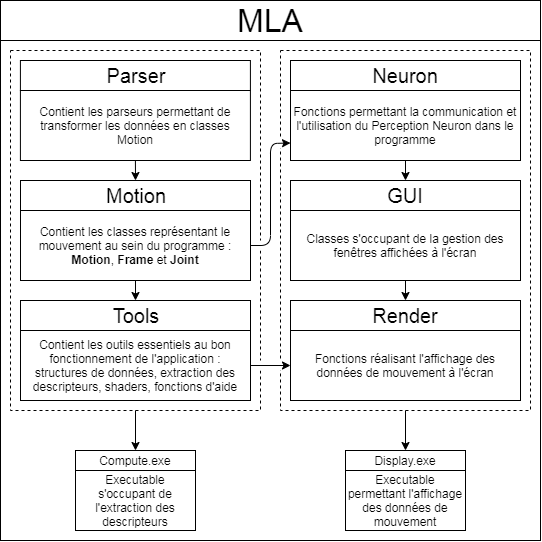
\includegraphics[width=\textwidth]{pictures/MLA_architecture.png}
    \caption[Architecture des pré-traitements et de l'affichage du mouvement capturé de \textit{MLA}]{L'architecture des pré-traitements et de l'affichage du mouvement capturé \textit{MLA}, divisée en six modules principaux.}
    \label{fig:MLA_architecture}
\end{figure}

\begin{figure}[h]
    \centering
    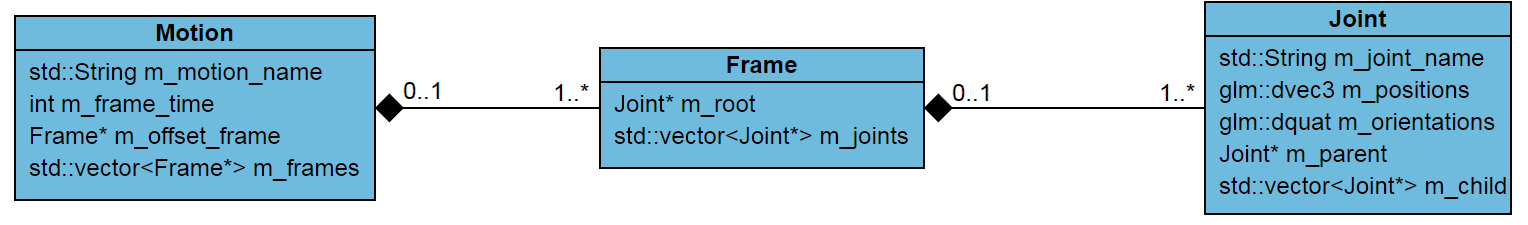
\includegraphics[width=\textwidth]{pictures/class_diagram_motion_MLA.png}
    \caption[Diagramme de classes du mouvement]{Diagramme de classes des trois classes composant le mouvement.}
    \label{fig:class_diagram_motion_MLA}
\end{figure}

Les descripteurs extraits du mouvement sont représentés au sein d'une structure \textbf{Data}, contenant le nom du descripteur, ainsi qu'un tableau contenant des couples de valeurs [nom de l'articulation] / [valeur du descripteur] (Fig. \ref{fig:class_diagram_datatype_MLA}). L'export de ces données se fait au format \textbf{JavaScript Object Notation} (\textbf{JSON}) (Fig. \ref{fig:json_data_example}), selon la hiérarchie suivante : descripteur $\rightarrow$ articulation $\rightarrow$ valeur. Le caractère peu-verbeux de ce format est un atout lors de l'export de fichiers de données volumineux. Sa très large utilisation, ainsi que le nombre conséquent d'analyseurs syntaxiques existants pour ce format en font un bon choix lorsque des données ont besoin de transiter d'une application à une autre \parencite{Gao2011JSON}. Il est ainsi possible de rechercher de manière naturelle (au sens du langage considéré) les descripteurs, en respectant le cheminement « descripteur $\rightarrow$ articulation ».

\begin{figure}[h]
    \centering
    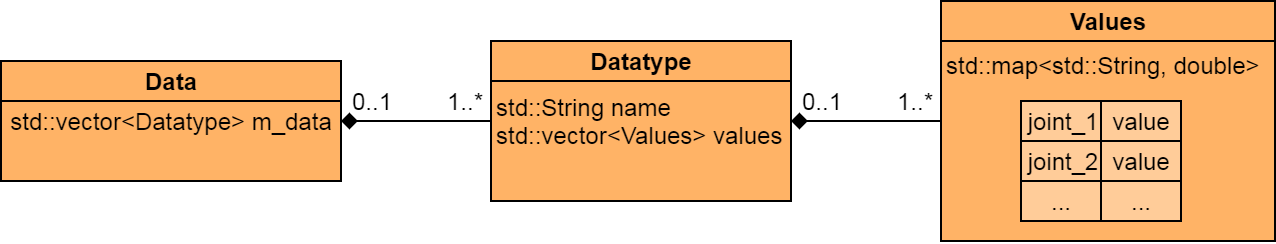
\includegraphics[width=\textwidth]{pictures/class_diagram_datatype_MLA.png}
    \caption[Diagramme de classes de la structure de stockage des données]{Diagramme de classes des classes composant la structure de stockage des données.}
    \label{fig:class_diagram_datatype_MLA}
\end{figure}

\begin{figure}[h]
	\centering
    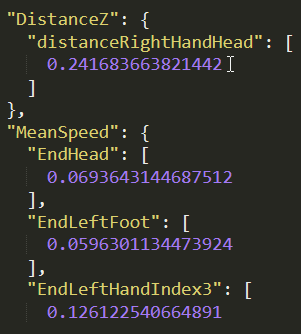
\includegraphics[]{pictures/json_data_example.png}
    \caption[Exemple de descripteurs au format JSON]{Un exemple de descripteurs extraits, au format JSON. Le stockage s'effectue selon la hiérarchie « descripteur $\rightarrow$ articulation $\rightarrow$ valeur ».}
    \label{fig:json_data_example}
\end{figure}

\subsection{Analyse automatique}
La partie Machine learning est codée en Python 3.6+. Le Python a été retenu comme langage pour le large choix de bibliothèques d'analyse de données et de machine learning.

L'objectif de cette partie est de proposer un ensemble d'outils permettant l'analyse des descripteurs extraits du mouvement capturé, à l'aide de techniques d'apprentissage non-supervisé. Il est possible de choisir un sous-ensemble d'articulations et de descripteurs à analyser à partir des données extraites, afin de concentrer l'analyse sur les parties du corps voulues. Un algorithme de \textit{clustering} est ensuite choisi, ainsi que les paramètres de cet algorithme. En fonction de l'algorithme, il est possible de modifier plusieurs paramètres : nombre de clusters (groupes) souhaités, taille du voisinage de recherche, \textit{etc.} Ce choix s'effectue pour l'instant par la personne gérant le programme, car le choix de l'algorithme et de ses paramètres doit se faire en fonction des données utilisées, et nécessite une connaissance scientifique. Des métriques sont ensuite calculées afin de fournir une indication quant à la qualité des regroupements obtenus. Il est possible de comparer les regroupements à un étiquetage des données, afin de vérifier si la séparation obtenue correspond aux \textit{a priori} de l'expert ou non. Cette phase de \textit{clustering} permet également d'obtenir deux groupes de mouvements : les mouvements cibles, et les mouvements avec défauts. Ces groupes sont ensuite utilisés pour donner un retour à l'apprenant.

\subsection{Feedback}
La partie feedback est également codée en Python 3.6+. L'objectif de cette partie du programme est de fournir un module proposant une aide à la décision pour un expert, mais également de proposer un retour compréhensible pour l'apprenant, dans le cas d'une utilisation sans expert. À partir de descripteurs pré-sélectionnés par l'expert lui-même, et d'exemples de mouvements réussis / ratés, le système fourni une aide visuelle afin de visualiser la différence entre les mouvements de l'expert et ceux de l'apprenant. L'objectif pour l'apprenant est de rapprocher le plus possible ses mouvements du groupe des mouvements cibles, en améliorant son geste au fur et à mesure de l'apprentissage, à l'aide des conseils dispensés par l'expert et/ou le système.\\


La plateforme MLA permet le traitement automatique de données de mouvement capturé, du filtrage au traitement automatique par des méthodes de \textit{clustering}, ainsi qu'à l'affichage synthétique d'information à destination de l'apprenant ou de l'expert. Cette partie a défini le contexte dans lequel s'incluent les travaux présentés dans cette thèse. Avoir une plateforme intégrant le traitement des données brutes, le calcul des descripteurs de mouvement, la comparaison et la visualisation des clusters de mouvements de l’apprenant possède l'avantage de centraliser les différentes étapes, et proposer ainsi un \textit{workflow} plus simple au sein d'un même artefact informatique. La suite de ce chapitre explique en détail le \textit{workflow} d'utilisation système.

\section{Capture de mouvement (Perception Neuron)}
Dans le cadre de cette thèse, la solution retenue pour la capture de mouvements a été celle de la combinaison de capteurs " Perception Neuron " \parencite{perceptionNeuron}, créée par l'entreprise NOITOM. Ce type de dispositif présente l'avantage d'offrir un compromis entre le coût et la qualité des données obtenues.

Le Perception Neuron est une combinaison de capteurs, basée sur l'utilisation de Neurons, des centrales inertielles (\textit{Inertial Measurement Unit}, ou \textbf{IMU} en anglais) composées d'un gyroscope, d'un accéléromètre et d'un magnétomètre. Ce type de capteur possède l'avantage d'être facilement portable par sa taille et son poids, et donc de présenter une gêne réduite pour l'utilisateur. Ces capteurs sont beaucoup utilisés dans le domaine médical \parencite{PORCIUNCULA2018S220}, pour l'analyse de la posture ou la rééducation d'une partie spécifique du corps par exemple.

Le Perception Neuron peut utiliser simultanément un ensemble de 32 Neurons au maximum. Les Neurons sont composés d'un accéléromètre, un gyroscope et un magnétomètre. Ces capteurs sont interchangeables, ce qui permet de ne changer que le Neuron défectueux si jamais un problème survient sur l'un d'entre eux. Cet ensemble de capteur est relié à un \textit{hub}, qu'il est possible de connecter à un ordinateur de manière filaire (liaison USB) ou non-filaire (WiFi). Le système est alimenté par un autre port USB, et il est possible d'utiliser une batterie USB rechargeable, afin d'obtenir une mobilité accrue. Il n'est possible d'utiliser le Perception Neuron que dans certaines configurations spécifiques (voir Fig. \ref{fig:perception_neuron_all_combinations}). Les données sont renvoyées à une cadence de 120 postures par secondes lorsque la combinaison est constituée de 17 Neurons ou moins, et de 60 postures par secondes lorsque le nombre de capteurs est supérieur ou égal à 18.

\begin{figure}
	\centering
    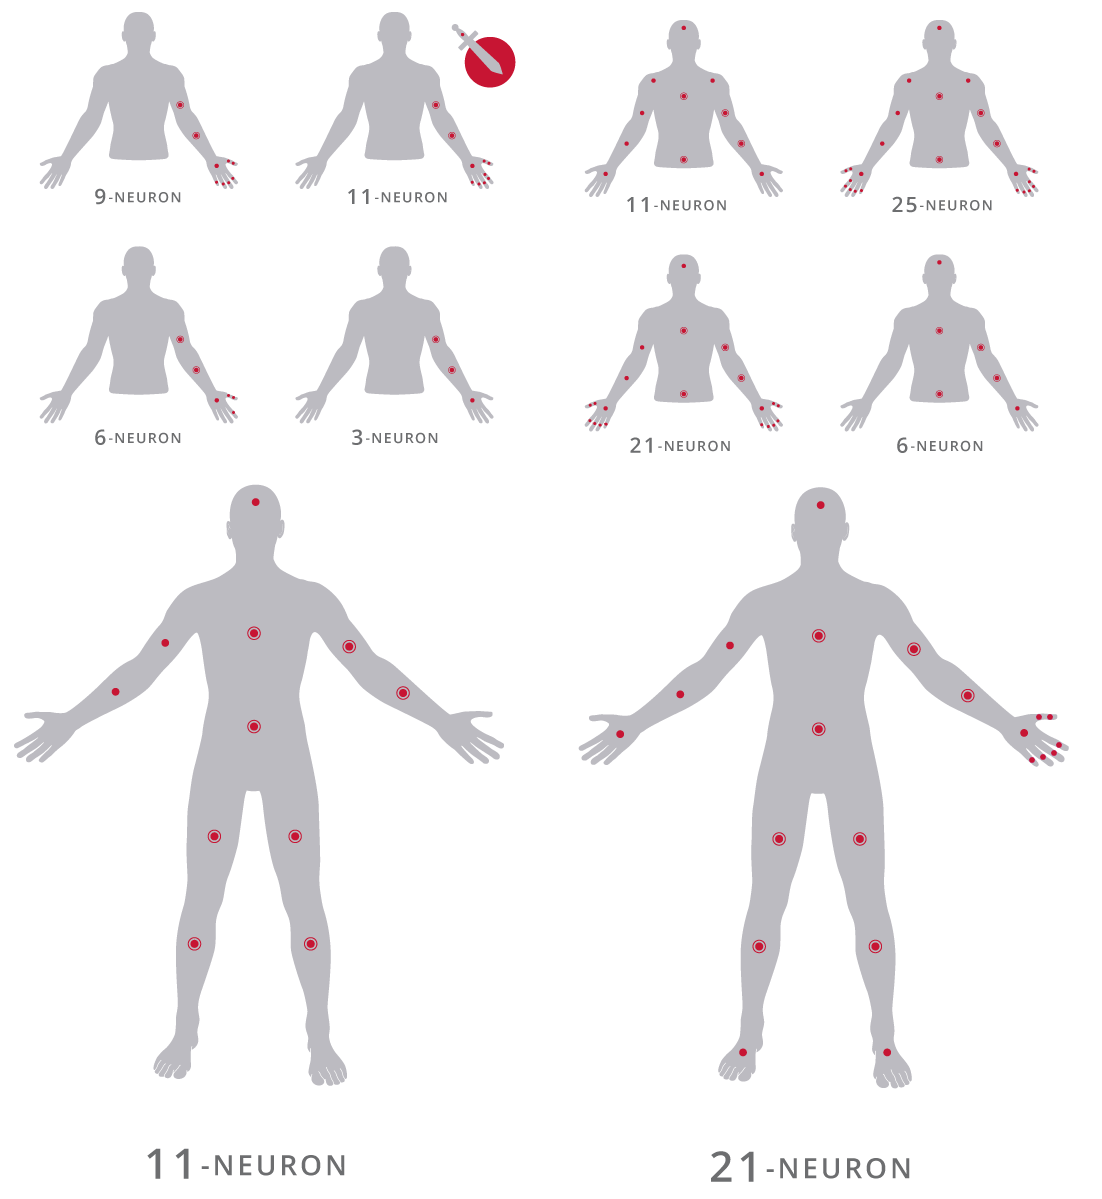
\includegraphics[width=\textwidth]{pictures/perception_neuron_all_combinations.png}
    \caption[Configurations possibles pour le Perception Neuron]{Toutes les configurations possibles pour le Perception Neuron \parencite{Noitom2015Doc}.}
    \label{fig:perception_neuron_all_combinations}
\end{figure}

Cette combinaison permet d'obtenir un squelette humain en 3D et donc d'éviter les problèmes propres aux  systèmes de capture vidéo 2D, en particulier celui de l'occlusion.

L'utilisation de cette combinaison nécessite l'utilisation du logiciel Axis Neuron, développé par NOITOM. Ce logiciel permet d'effectuer la communication entre le hub de la combinaison et l'ordinateur. Il est également le seul capable de lire le format de données dans lequel est enregistré le mouvement. Il permet de réaliser les calibrations de la combinaison, de visualiser en temps réel le mouvement réalisé, de rejouer un mouvement (avec possibilité de marche avant / marche arrière, ralentissement, etc.), d'utiliser différents squelettes afin de s'adapter à toutes les morphologies possibles, et d'éditer le mouvement.

\section{Pré-traitements des données}
Bien que présentant de nombreux avantages, les centrales à inertie ne sont cependant pas dénuées de problèmes \parencite{Giansanti2003Iif}. Le phénomène de la dérive (\textit{drift} en anglais) est le plus courant : il s'agit de l'accumulation d'erreurs d'intégration, qui sert à obtenir l'information d'orientation de position à un temps $T$ à partir de la vitesse, elle-même déduite de l'accélération. Les capteurs magnétiques sont également sensibles aux perturbations extérieures : la présence d'objets métalliques, ou d'objet émettant un champ électromagnétique. Ces phénomènes combinés font que les données obtenues lors des captures de mouvements ne sont pas toujours précises. La différence entre le geste réalisé par une personne et le geste visualisé sur le logiciel Axis Neuron est parfois très grande. De plus, le logiciel Axis Neuron applique des traitements aux données reçues des capteurs. Ils sont au nombre de trois : \textit{Embeded Data Fusion}, \textit{Human Body Dynamics} et \textit{Physical Engine}. Ces algorithmes sont propriétaires, et donc non documentés de manière exhaustive : il est très difficile de savoir dans quelle mesure les données sont modifiées avant d'être présentées dans le logiciel. À cause de cette limitation, des corrections de données ont été effectuées sur les descripteurs extraits du mouvement, et non sur le mouvement original lui-même. Dans les parties suivantes, nous traitons des signaux. Le terme \textit{artefacts} sera ici utilisé pour décrire les erreurs présentes au sein de ces signaux, dues au matériel de capture, et non pour parler d'un artefact informatique.

\section{Traitements des données de mouvement}\label{sec:traitements}
Dans le cadre de tests du système, des mouvements de lancers ont été utilisés afin d'en extraire des descripteurs. Ces descripteurs était relatifs aux vitesses de la main. Un des premiers tests du système a été la vérification de la cohérence de ces descripteurs par rapport au mouvement réel. Lors de l'extraction d'informations à partir des données de mouvement, il a été remarqué que les vitesses extraites à partir des positions successives présentaient des \textit{artefacts} conséquents (Fig. \ref{fig:linear_speed_artifacts}). Ces \textit{artefacts} se retrouvent le plus souvent lorsque des changements brusques de vitesse se produisent, c'est-à-dire quand l'accélération augmente ou décroit rapidement. Il n'est pas possible d'utiliser des données présentant ces défauts sans une étape de correction. L'analyse de l'origine de ces \textit{artefacts} a permis de mettre au jour deux problèmes majeurs des données de mouvement provenant du logiciel Axis Neuron : le changement de la taille des membres du squelette au cours du temps, et les problèmes d'incohérences de changement de position d'une frame à une autre.

\begin{figure}
	\centering
    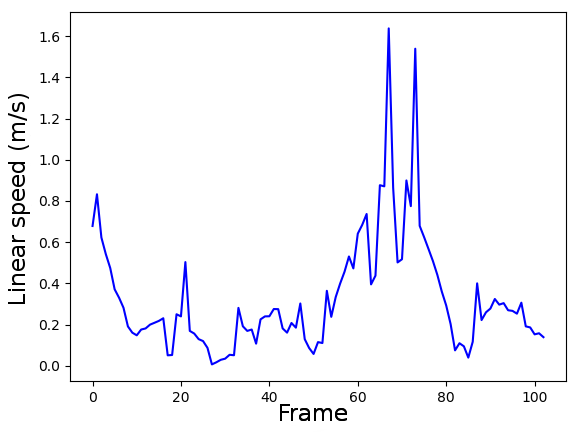
\includegraphics[width=7.5cm]{pictures/linear_speed_artifacts.png}
    \caption[Vitesse linéaire avec artéfacts]{Un exemple de vitesse linéaire extraite d'un mouvement. On remarque bien les pics de vitesse (autant vers le haut que vers le bas) entre les frames 60 et 80 (abscisses), ne correspondant pas à un lancer fluide.}
    \label{fig:linear_speed_artifacts}
\end{figure}

\subsection{Variation de la taille des membres}
Un des premiers problèmes rencontrés a été la variation de la taille des membres du corps au cours du mouvement. Il apparaît que la taille des membres ne reste pas fixe tout au long du lancer. Ce problème peut provenir soit de l'imprécision des capteurs, soit des traitements effectués avant la restitution du mouvement.

Une solution simple est de fixer cette taille, qui correspond à l'écartement entre les articulations, pour chaque membre. Pour chaque enregistrement, il existe une posture de référence, qui contient toutes les informations de position et d'orientation pour chaque articulation. Cette \textit{frame} est créée après la phase de calibration, ce qui fait qu'elle est moins sujette aux problèmes inhérents aux capteurs, car ces derniers surviennent au bout d'un certain temps de captation.

Pour chaque articulation, les informations sont stockées sous la forme d'un vecteur de dimension 3, correspondants aux positions de l'articulation en $x, y, z$, et d'un quaternion correspondant à la rotation de cette articulation. Ces informations sont données par rapport à l'articulation parente : les valeurs de position et d'orientation d'une articulation fille $j_{i+1}$ sont donc données relativement à l'articulation mère $j_i$, et la position de l'articulation fille $p_{j_{i+1}}$ correspond donc à la taille du membre $m_{j, j+1}$. La première étape du traitement des données par la plateforme MLA consiste donc à copier les positions de l'articulation de la frame de référence sur toutes les autres frames du mouvement. L'orientation reste inchangée.

\subsection{Incohérences de position des articulations d'une frame à une autre}

Un autre défaut présent dans les données a été constaté lorsque les vitesses ont été extraites des mouvements. Dans le cadre de tests, un mouvement de lancer a été enregistré, afin d'en extraire des descripteurs. Il s'est avéré que les valeurs de vitesses pouvaient parfois varier grandement d'une \textit{frame} à une autre, sans pour autant que cette variation ne soit représentative du mouvement réel (Fig. \ref{fig:linear_speed_artifacts}). En effet, lors du lancer test, et après observation de l'enregistrement vidéo correspondant à ce lancer, il apparaît que les variations de vitesses très brèves (correspondantes aux pics vers le haut et vers le bas du signal) ne correspondaient pas à la réalité du mouvement. À l'œil nu, lorsque le mouvement est affiché à l'écran, ces erreurs ne sont pas visibles, car ces variations apparaissent sur des temps très courts (de l'ordre du centième ou du millième de seconde). Cependant, lors de l'extraction de la vitesse, il apparaît que la variation est parfois extrême sur un ensemble de frames données.

Nous avons formulé quatre hypothèses pour expliquer ces incohérences de non-linéarité dans le mouvement :
\begin{enumerate}
	\item Le pas de temps entre les \textit{frames} est constant, et l'interpolation entre ces \textit{frames} est incorrecte, ce qui signifie que l'implémentation de l'interpolation entre les \textit{frames} est mal réalisée au sein du logiciel Axis Neuron.
	\item Le pas de temps entre les \textit{frames} est constant, et il n'y a pas d'interpolation, ce qui signifie qu'il manque des \textit{frames}. Ce problème pourrait subvenir lorsque la combinaison n'arrive pas à retourner les données des capteurs, à cause du trop grand nombre de données à traiter en simultané et en temps réel.
	\item Le pas de temps entre les \textit{frames} n'est pas constant et il y a interpolation, ce qui signifie que l'interpolation est incorrecte à cause d'un mauvais indice temporel donné à la \textit{frame} reconstituée. Supposons un mouvement linéaire composé de trois frames $f_0, f_2, f_4$ prises aux temps $t_0, t_{0+2}, t_{0+4}$ respectivement. Si le système ne renvoie que les informations des frames $f_0$ et $f_4$, l'interpolation entre la première frame $f_0$ et la deuxième frame $f_4$ reçue, étant supposée correspondre à l'instant $t_{0+1}$, correspondra en fait au moment $t_{0+2}$.
	\item Le pas de temps entre les frames n'est pas constant, et il n'y a pas d'interpolation, ce qui signifie qu'il manque des frames. Supposons un mouvement linéaire composé de cinq frames $f_0, f_1, f_2, f_3, f_4$ prises aux temps $t_0, t_{0+1}, t_{0+2}, t_{0+3}, t_{0+4}$ respectivement. Si le système ne renvoie que les informations des frames $f_0$, $f_1$, $f_3$ et $f_4$, il y aura un déplacement entre les frames $f_1$ et $f_3$ correspondant à $2*t$.
\end{enumerate}

Le tableau \ref{linear_speed_problem_hypothesis_table} résume ces hypothèses.
\begin{center}
\begin{table}[h!]
\begin{tabular}{l|l|l}
& \makecell{Interpolation} & Pas d'interpolation \\\hline
\makecell{Intervalle de temps\\constant} & \makecell{Mauvaise interpolation} & \textit{Frames} manquantes                  \\\hline
\makecell{Intervalle de temps\\non-constant} & \makecell{Mauvaise posture\\dû a un indice temporel erroné} & \makecell{\textit{Frames} affichées\\au mauvais moment}
\end{tabular}
\caption{Résumé des hypothèses sur les incohérences de positions}
\label{linear_speed_problem_hypothesis_table}
\end{table}
\end{center}

Il est possible que ces erreurs proviennt d'une baisse de la fréquence de retour des donneés, ou d'un problème d'acquisition des capteurs. En effet, sur le logiciel Axis Neuron®, chaque capteur possède un indicateur visuel permettant de juger de la qualité des données retournées : vert (OK), jaune (moyen), rouge (mauvais). Il n'existe cependant aucune indication sur la nature des dégradations des données. Indépendament de la cause, il est possible de proposer des solutions permettant de pallier ce problème. Ces constatations font qu'il était nécessaire de trouver une manière de nettoyer les données avant leur utilisation. Plusieurs pistes ont été évoquées. Il serait possible de reconstruire le mouvement par interpolation, avec un pas de temps fixe. En prenant un pas de temps suffisamment grand, on peut espérer obtenir un mouvement recomposé évitant les sauts de distance. Cependant, en faisant ainsi, le nombre de \textit{frames} du mouvement recomposé sera bas, et le mouvement recomposé risque de passer outre des moments clés du mouvement original (flexion d'une partie du corps, variation de l'accélération, etc.). Il existe des techniques d'interpolation se basant sur des \textit{frames} clés (\textit{key-frames}), afin de garder les informations cruciales du mouvement \parencite{Brotman1988MIO}. Cette méthode nécessite de définir ces \textit{frames} clés à l'avance. Or, au vu du nombre de données à traiter, il est difficile de spécifier manuellement ces frames clés pour chaque mouvement enregistré.

Les descripteurs vitesses extraits à partir du mouvement originel présentaient donc des \textit{artefacts}. De par les caractéristiques propres à ces \textit{artefacts} (pics très intenses et de courte durée), un filtre a été appliqué sur les valeurs de vitesses ainsi obtenues. Cette étape est cruciale, car les valeurs de vitesses sont utilisées plus tard dans la chaine de traitement afin de segmenter le mouvement.

Il existe plusieurs types de filtres pouvant être appliqué à un signal, afin d'en réduire le bruit. Rojas-Lertxundi \textit{et al.} présentent plusieurs de ces filtres dans \parencite{Rojas2015MCS}. Parmi eux, le filtre passe-bas a été utilisé par Kristianslund \textit{et al.} \parencite{KRISTIANSLUND2012Eol} afin de filtrer les signaux provenant des mouvements des articulations de joueurs de handball et d'améliorer la détection et la prévention de blessures. Le filtre de Butterworth est un filtre qui possède un gain constant dans sa bande passante. Il a été utilisé par Malfait \textit{et al.} \parencite{Malfait2014Hra} afin de filtrer des données de test de détente. Les filtres de Chebyshev sont des filtres qui proposent une plus grande ondulation soit en bande passante (Type I) soit en bande atténuée (Type II) que les filtres de Butterworth. Il a été utilisé par Fanis et Stathis \parencite{Moschas2011Mot} afin de réduire le bruit provenant de données GPS et d'accéléromètre. Le filtre de Kalman repose sur le principe de l'estimation de données à partir de l'observation de données bruitées. Ces filtres sont très utilisés pour filtrer les données provenants d'IMUs \parencite{Zihajehzadeh2014Act} \parencite{Marins2001AeK} \parencite{Luinge1999Eow}. Le filtre de Savitsky-Golay est un filtre passe-bas servant à lisser une courbe \parencite{Savitsky1964SaD}. Il se base sur une fenêtre glissante, et effectue une régression afin de déterminer le polynôme minimisant l'erreur au sens des moindres-carrés pour un point donné. Plus cette fenêtre est large, plus le signal sera lisse, et plus les pics courts seront atténués. Le degré de ce polynôme dépend du cas applicatif : un polynôme de degré 2 permet de prendre en compte une courbure dans le signal, alors qu'un polynôme de degré 3 permet de prendre en compte les points d'inflexion du signal.

Ce filtre a été retenu, de par sa simplicité de compréhension, sa rapidité d'exécution et également son principe de réduction du bruit (à l'inverse du filtre Kalman, qui lui trouve des informations au sein d'un signal bruité). De plus, bien que le filtre de Kalman semble être un candidat judicieux au vu du matériel utilisé, il est habituellement utilisé pour traiter les données de mouvement provenant directement des capteurs, et non les descripteurs extraits de ces derniers.

La détermination des paramètres de ce filtre s'est effectuée de manière empirique. La taille de la fenêtre symétrique correspond à $\frac{T}{4}$, avec $T$ étant la durée totale de l'enregistrement du mouvement. Le polynôme utilisé est de degré $3$ : une valeur inférieure lisse trop les données, et résulte en une perte d'information, alors qu'une valeur supérieure créée un sur-ajustement \ref{savgol_comparison_all_3_at_once}. Il a été déterminé empiriquement qu'une taille de fenêtre de $ \frac{nbframes}{4}$ permettait d'obtenir un signal lissé, sans pour autant en gommer les caractéristiques principales.

\begin{figure}
	\centering
    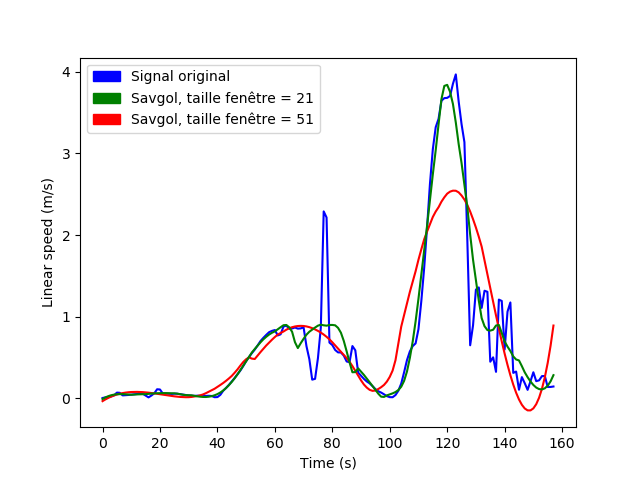
\includegraphics[width=\textwidth]{pictures/savgol_comparison_all_3_at_once.png}
    \caption[Comparaison de l'influence des paramètres d'un filtre Savitsky-Golay]{Un exemple de filtrage de données de vitesses par un filtre de Savitsky-Golay. Le signal original est en bleu, suivit par les résultats du filtrage avec une taille de fenêtre de 21 en vert) et une taille de fenêtre de 51 (en rouge). Une taille de fenêtre trop élevée efface tous les artefacts présents, mais gomme également les caractéristiques propres du signal (le changement brusque de vitesse).}
    \label{savgol_comparison_all_3_at_once}
\end{figure}

L'application de ce filtre sur les données de vitesse bruités (Fig. \ref{fig:before_after_savgol}) permet d'obtenir une courbe plus lisse, se rapprochant d'avantage de la réalité de la vitesse du mouvement effectué. La courbe de vitesse lors du lancer correspond aux enregistrements, et il est également possible de distinguer les gestes d'amplitude plus faible précédent le lancer (dans le cas présent, il s'agit de l'étape de balancement de la main avant le lancer, voir Fig. \ref{fig:after_savgol_explained}).

\begin{figure}
	\centering
    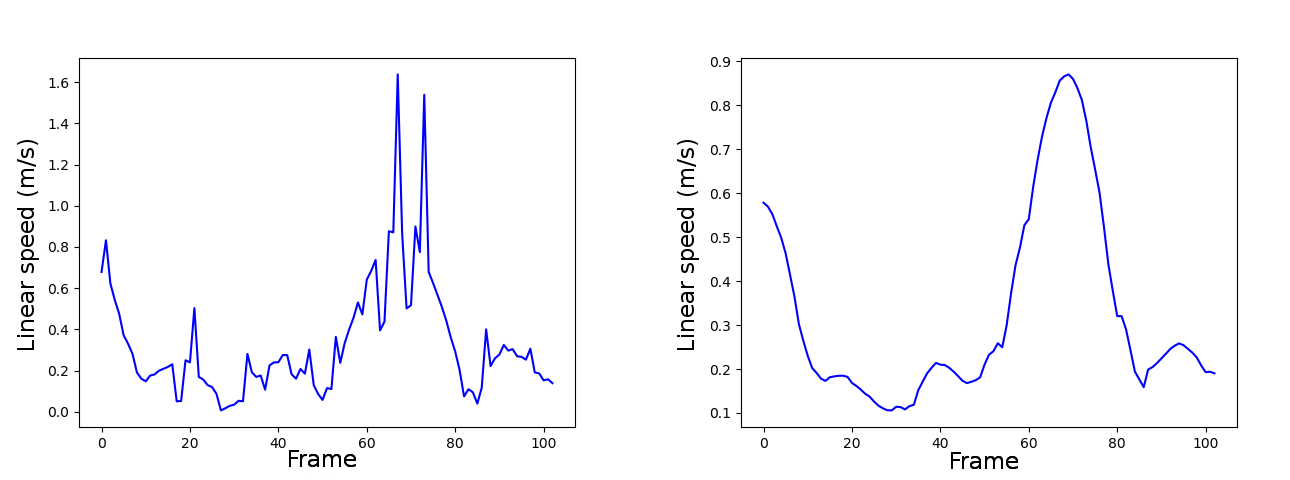
\includegraphics[width=\textwidth]{pictures/before_after_savgol.png}
    \caption[Vitesses filtrées par un filtre de Savitsky-Golay]{Un exemple de vitesse linéaire filtrée (à droite) à l'aide d'un Savitsky-Golay. Les pics correspondants aux artefacts du mouvement on disparu, et les caractéristiques initiale du changement de vitesses ont été conservées.}
    \label{fig:before_after_savgol}
\end{figure}

\subsection{Extraction du moment d'intérêt du mouvement}\label{subsec:MoI}
Lors de l'analyse d'un mouvement, il n'est pas systématiquement nécessaire de disposer de l'intégralité du mouvement. Par exemple, dans le cadre d'un service au tennis, l'analyse du mouvement se concentre sur les parties hautes du corps, notamment le poignet de la main qui tient la raquette \parencite{Makio2007DoS}. Il est également possible que le mouvement jugé utile soit contenu au sein d'un enregistrement plus large : il faut alors être capable d'extraire le mouvement d'intérêt. Segmenter manuellement un mouvement est une tâche réalisable par un humain. Cependant, en fonction du nombre de données à traiter, de la durée totale des mouvements, du nombre de passages à segmenter, cette tâche peut devenir chronophage. La segmentation automatique du mouvement peut pallier ce problème.

Il existe plusieurs techniques de segmentation automatique du mouvement \parencite{Zappella2008MSR}. L'ensemble des techniques permettant cette segmentation se basent sur différentes méthodes : apprentissage supervisé / non-supervisé, réduction de dimension, etc. Le choix de la méthode se base souvent sur la connaissance \textit{a-priori} des caractéristiques propres au mouvement. Les techniques à base d'apprentissage supervisé supposent que les classes (\textit{i.e.} les types de mouvements présents au sein du corpus) soient connues en amont. À l'inverse, les techniques non-supervisées ne possèdent pas d'\textit{a-priori} sur le type du mouvement : la segmentation se fait sans assignation à une classe.

Les méthodes de segmentation à base d'apprentissage supervisé se basent sur un corpus d'apprentissage correspondant au sous-mouvement à extraire du mouvement principal. Ces méthodes proposent souvent à la fois une segmentation en actions et une classification de ces actions. En entrainant des classifieurs sur des séquences choisies avec soin au préalable, il est possible d'obtenir une segmentation du mouvement, en fonction des différentes actions présentes. Les méthodes peuvent faire appel à des classifieurs SVM \parencite{Hoai2011Seg}, des modèles de markov cachés (\textit{Hidden Markov Models}, \textit{HMM}) et une combinaison de classifieurs faibles afin de créer un classifieur fort (Multi-class Adaboost) \parencite{Fengjun2006Ada}, ou encore des réseaux de neurones \parencite{Bouchard2007SSM}. Ces méthodes nécessitent toutes un corpus préalablement constitué, étiqueté et sont le plus souvent testées sur des corpus de mouvements existants et connus, tels que CMU \parencite{CMUDatabase} et HDM05 \parencite{HDM05Database}. Ces bases sont constituées de nombreux mouvements, tels que se lever, s'asseoir, prendre un objet, etc. Ces mouvements ne nécessitent pas d'effort cognitif particulier pour un humain, et donc ne sont pas sujet à un quelconque apprentissage. De plus, lorsque le domaine métier ne dispose pas de base de mouvements pré-établie, il faut en constituer une en disposant de suffisamment d'exemples étiquetés, et couvrant une grande variété de cas (différences de morphologie, de durée, de manière de faire, etc.).

La segmentation de mouvement par l'approche à base d'apprentissage non-supervisé permet de s'affranchir de certaines de ces contraintes. L'objectif reste le même, à savoir décomposer un mouvement en plusieurs sous-mouvements, mais cette fois sans \textit{a-priori} sur ces séparations. Trois méthodes ont été proposées par Barbi \textit{et al.} \parencite{Barbic2004SMC}, traitant toutes le mouvement comme étant une séquence ordonnée de \textit{frames}. A partir des données de rotation (quaternions), une analyse en composantes principales (\textit{PCA}) de ces données est réalisée sur chaque \textit{frame}, afin d'obtenir une représentation de plus basse dimensionnalité. Cette approche se base sur le fait qu'un mouvement simple aura une représentation de basse dimensionnalité. En minimisant l'erreur de projection, la dimensionnalité optimale est trouvée. En calculant ensuite la dérivée des valeurs succesives de l'erreur, il est possible de détecter les fractures au sein du mouvement, \textit{i.e.} là où la dérivée augmente fortement. La deuxième méthode se base sur l'analyse en composantes principales probabilistes (\textit{PPCA}) \parencite{Tipping1999PPCA}. Les premières \textit{frames} du mouvement sont modélisées sous forme d'une distribution Gaussienne, en fonction de la dimension intrinsèque estimée. La probabilité d'appartenance des \textit{frames} suivantes à la distribution Gaussienne est ensuite calculée, à l'aide d'une distance de Mahalanobis. En augmentant progressivement le nombre de frames utilisées pour le calcul de la distribution Gaussienne, il est possible d'obtenir une courbe de la distance calculée à chaque fois. Les pics de cette courbe apparaissent lorsqu'un changement de comportement survient : il s'agit du moment où le mouvement change, et donc où la segmentation va prendre place. La dernière technique proposée dans ces travaux se base sur un modèle de mélange de gaussiennes (\textit{GMM}). L'hypothèse de départ est que les frames de différents mouvements simples vont former différents clusters. Le PCA est utilisé afin de réduire les temps de traitements de l'algorithme d'estimation, et le nombre de composantes à garder est choisi afin que $90\%$ de la variance de la distribution des données originale soit préservée. Une fois les paramètres du modèle estimés, un cluster d'appartenance est calculé pour chaque \textit{frame}. L'inconvénient de cette méthode est qu'il faut spécifier à l'avance le nombre de clusters.

Une autre technique utilise l'analyse de clusters alignés, afin d'obtenir une segmentation du mouvement \parencite{Zhou2008ACA}. Cette méthode réduit le problème de la segmentation à un problème de \textit{clustering}. Elle est basée sur l'algorithme des \textit{k-means}, et propose deux changements majeurs par rapport à cet algorithme : la taille des caractéristiques d'un cluster peut varier, et la fonction de distance utilisée se base sur la déformation temporelle dynamique (\textit{DTW}). Cette technique permet de calculer une similarité entre deux séries temporelles, tout en étant robustes aux décalages de phase sur l'axe du temps \parencite{Berndt1994DTW}. Afin d'appliquer cette segmentation à de larges corpus, il est nécessaire d'opérer une réduction du nombre de \textit{frames} initiales.

La granularité de la décomposition peut grandement varier. Ainsi, la méthode développée par Krüger \textit{et al.} \parencite{Kruger2017EUT}, en utilisant en premier lieu du regroupement de caractéristiques, puis ensuite le voisinage des graphes constitués par les caractéristiques propres à chaque \textit{frame}, permet non seulement de séparer différentes actions au sein d'un mouvement initial (par exemple, une personne qui marche puis qui se met à courir), mais également de subdiviser encore les sous-mouvements obtenus en primitives (par exemple, les pas individuel lors de la marche et de la course).

%La segmentation obtenue est souvent dénuée de sémantique, bien que des études permettent d'obtenir dans un premier temps la segmentation, puis dans un deuxième temps de relier cette division à des étiquettes

Bien que les techniques précédemment présentées atteignent des bons taux de segmentation (par rapport à la segmentation manuelle), la solution retenue est plus simple, et se base sur les pics de vitesses du mouvement. Cet algorithme permet une segmentation rapide des mouvements, dès lors que le mouvement d'intérêt présente une forte variation de vitesse. Les mouvements caractéristiques des expérimentations sont le passage d'une vitesse quasi-nulle (position stationnaire), ou d'une vitesse faible (mouvement de balancier avant le lancer), a une vitesse élevée (mouvement du lancer), puis au retour à une vitesse faible, voire nulle (position de repos). La solution retenue permet ainsi une bonne segmentation du mouvement d'intérêt (\textit{Motion of Interest}, \textit{MoI}). L'algorithme de segmentation qui a été développé se base sur un repérage de la valeur maximale de la vitesse d'une articulation pré-déterminée. Dans le cas d'étude présenté, la main est l'articulation choisie, car nous nous plaçons dans le cas de mouvements de lancer, et cette articulation est source de la plus grande amplitude en terme de positions. Il serait cependant possible de déterminer automatiquement quelle articulation présente la plus grande amplitude de variations de vitesses, et de trouver ainsi le pic de vitesse maximale lors du geste. En partant de ce maximum, la segmentation s'effectue en choisissant un nombre de minimum locaux à franchir avant et après ce maximum. Ce choix permet d'intégrer au \textit{MoI} les phases de balancement pré-lancer, par exemple. Dans notre cas, nous nous limitons au \textit{MoI} seul. L'algorithme ainsi choisi (Algorithm \ref{algorithm_MoI}) permet de limiter la consommation de ressources (temps et mémoire).

\begin{algorithm}
\caption{MoI extraction algorithm}
\begin{algorithmic}[1]
\State $motion$: the full motion
\State $lc$: the number of desired left cuts
\State $rc$: the number of desired right cuts
\Procedure{Motion segmentation}{$motion$, $lc$, $rc$}
	\State $hs \gets$ GetHighestSpeedValue($motion$)
    \State $p\_lm \gets$ GetPreviousLocalMin($hs$)
    \State $n\_lm \gets$ GetNextLocalMin($hs$)
    \State $left\_found$ = 0
    \State $right\_found$ = 0
    \State $seg\_motion \gets$ segmented motion from $p\_lm$ to $n\_lm$
 	\While{$left\_found$ < $lc$}
          \State $n\_lm$ = $p\_lm$
          \State $p\_lm \gets$ GetPreviousLocalMin($p\_lm$)
          \State $seg\_motion \gets$ $motion$ from $p\_lm$ to $n\_lm$ added at the beginning
  	\EndWhile

    \While{$right\_found$ < $rc$}
          \State $p\_lm$ = $n\_lm$
          \State $n\_lm \gets$ GetNextLocalMin($n\_lm$)
          \State $seg\_motion \gets$ $motion$ from $p\_lm$ to $n\_lm$ added at the end
  	\EndWhile

 \EndProcedure
 \end{algorithmic}
 \label{algorithm_MoI}
\end{algorithm}

\begin{figure}
	\centering
    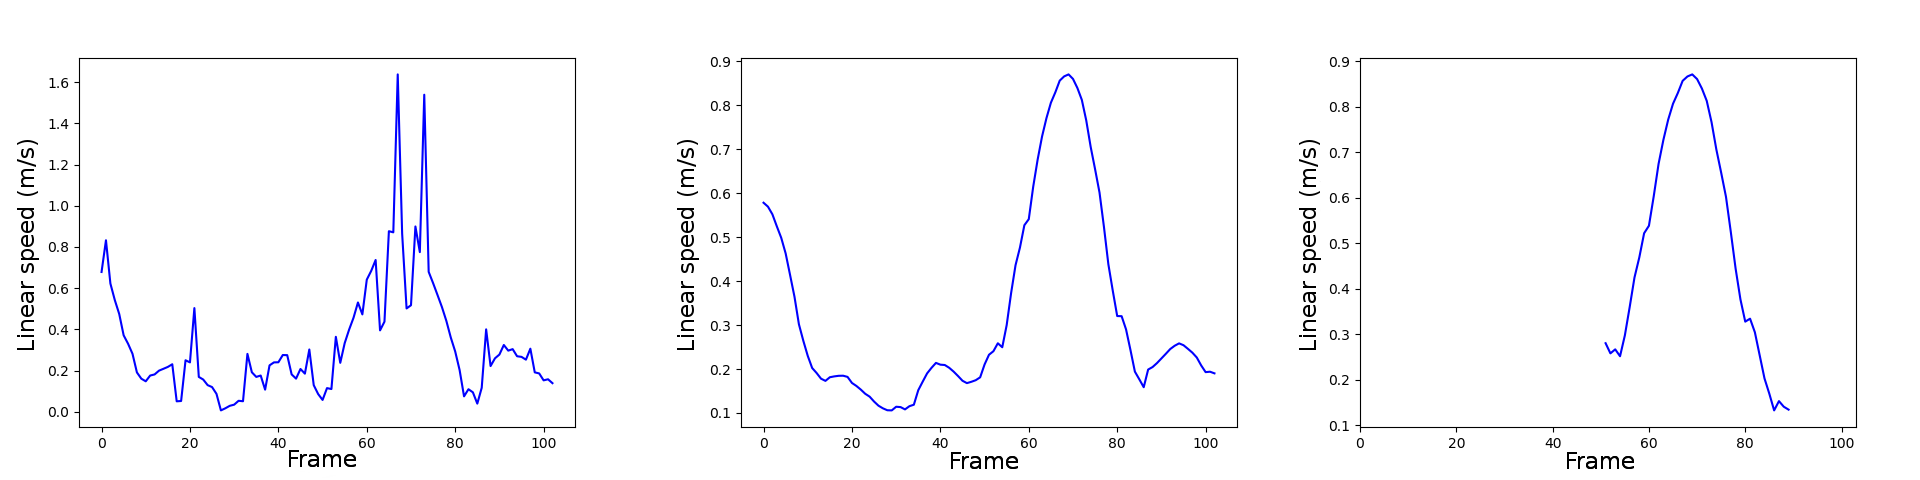
\includegraphics[width=\textwidth]{pictures/speed_values_all.png}
    \caption[Vitesse linéaire filtrée et segmentée]{Un exemple de vitesse linéaire filtrée puis segmenté par l'algorithme \ref{algorithm_MoI}.}
    \label{fig:speed_values_all}
\end{figure}

Cette étape marque la fin de la chaîne de pré-traitement des données de mouvement. En sortie de cette chaîne, un mouvement filtré et segmenté est proposé, afin de n'extraire les descripteurs que des parties d'intérêt du mouvement (Fig. \ref{fig:speed_values_all} et \ref{fig:after_savgol_explained}).

\begin{figure}
	\centering
    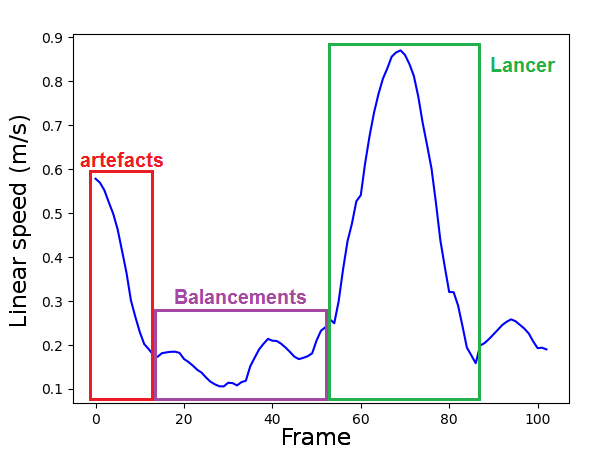
\includegraphics[width=10cm]{pictures/after_savgol_explained.png}
    \caption[Signal filtré décomposé en trois étapes]{Le signal filtré décomposé. En rouge, des artefacts de vitesses élevées dues aux capteurs. En violet, les balancements pré-lancer, et en vert, le lancer qui est extrait.}
    \label{fig:after_savgol_explained}
\end{figure}

\subsection{Aide à l'expert et retour à l'apprenant}\label{subsec:feedback}
À partir des descripteurs préalablement extraits, cette partie du système se concentre sur la comparaison des données expertes avec celles de l'apprenant, afin de fournir un retour sur les mouvements effectués. L'objectif est d'assister l'expert dans sa tâche d'évaluation du geste, en lui permettant d'obtenir un retour visuel sur les différences entre le geste de l'apprenant et le sien. Cela nécessite d'avoir des données expertes qui correspondent au geste cible, ainsi qu'un jeu de données pour chaque défaut à détecter au sein du mouvement. L'algoritme \ref{algorithm_Feedback} présente le cheminement. À partir des données de l'expert (réparties en gestes cibles et en mauvais gestes) et de l'apprenant, les données sont normalisées si nécessaire. Ensuite, une liste de descripteurs à observer pour chaque défaut identifié est demandée, afin d'associer les-dits descripteurs aux données de l'expert. Les données de l'expert sont ensuite utilisées dans un processus de \textit{clustering}, afin d'obtenir deux groupes, correspondants aux gestes cibles et aux mauvais gestes. Les données de l'apprenant sont ensuite comparées à celles de l'expert, afin d'être en mesure de déterminer quels sont les défauts à corriger en priorité pour l'apprenant. Enfin, un retour sous forme visuelle, présentant les données de l'expert et celle de l'apprenant, est proposé à l'expert, ainsi que possiblement des conseils des données par le système.

Ce système nécessite des données d'expert qui doivent contenir à minima : (i) des exemples de bons mouvements, et (ii) des exemples de mouvements présentant des défauts. Idéalement, les mouvements avec les défauts de l'expert doivent couvrir le plus d'exemples possibles pour chaque défaut. L'étiquetage marquant les bons et mauvais gestes de ces données doit être explicitement donnée au système, afin qu'il soit possible de faire correspondre un jeu de donnée avec un défaut. Il faut ensuite fournir une liste des descripteurs à observer, pour chaque défaut. Il est possible d'utiliser n'importe quelle combinaison d'articulation en fonction des besoins d'observation.

Il faut ensuite choisir quelles données seront utilisées pour la comparaison, autant pour l'expert que l'apprenant. La spécification de chaque type de données se fait de la manière suivante :
\begin{enumerate}
	\item le défaut pour lequel ce(s) descripteur(s) est/sont considéré(s)
	\item le descripteur à utiliser
	\item le(s) articulation(s) à considérer pour ce descripteur, avec pour chaque articulation la prise en compte ou non de la latéralité de la personne (e.g. si il faut remplacer " droite " par " gauche " dans le nom des articulations si la personne est gauchère)
\end{enumerate}

Ainsi, un exemple d'une telle spécification peut ressembler à la hiérarchie suivante :
\begin{itemize}[label=\textbullet]
	\item Défaut : Se pencher en avant lors du lancer
	\begin{itemize}[label=\textbullet]
		\item Descripteur : Vitesse moyenne
		\begin{itemize}
			\item Articulation : Épaule gauche, Latéralité : Non
		\end{itemize}
		\begin{itemize}
			\item Articulation : Épaule droite Latéralité : Non
		\end{itemize}
	\end{itemize}

	\item Défaut : Déplacement du coude lors du lancer
	\begin{itemize}[label=\textbullet]
		\item Descripteur : Vitesse moyenne
		\begin{itemize}
			\item Articulation : Bras gauche Latéralité : Oui
		\end{itemize}
		\begin{itemize}
			\item Articulation : Épaule gauche Latéralité : Oui
		\end{itemize}
	\end{itemize}
\end{itemize}

Les données peuvent être normalisées. En effet, le fait d'avoir des données sur plusieurs échelles différentes fait que certaines données peuvent devenir prédominantes dans le cas d'une analyse. Prenons l'exemple d'un descripteur $A$ dont les valeurs vont de $0$ à $5$, et d'un descripteur $B$ dont les valeurs vont de $500$ à $1500$. Dans ce cas, les variations du descripteur $A$ seront toujours insignifiantes comparées aux variations du descripteurs $B$, si les valeurs de chaque descripteur couvrent leurs intervalles respectifs de la même manière. L'étape de normalisation permet de mettre les données sur une même échelle, annulant par la même occasion les différences de plages de valeurs. Cette étape est cruciale lorsque les descripteurs utilisés ont une plage de valeur très différente les uns par rapport aux autres. Cette normalisation s'effectue en divisant chaque valeur composant les vecteurs de caractéristiques par la moyenne de ces valeurs au sein des données utilisées. Elle intervient avant le processus de clustering.

Les données de l'expert sont ensuite passées dans une phase de clustering (algorithme des \textit{k-means}, avec $k = 2$). Cette étape permet de constituer deux groupes de données : le groupe correspondant aux bons gestes, et le groupe correspondant aux gestes avec des défauts. Une première approche serait de faire ce regroupement à l'aide de l'étiquetage des données. Cependant, un problème de cette approche est qu'elle suggère que l'expert a fourni un ensemble de données où les gestes possédant des défauts sont séparables des bons mouvements. En pratique, il arrive que lorsque l'expert effectue plusieurs gestes avec un même défaut de suite, un phénomène d'auto-correction apparaît : inconsciemment, son geste va se rapprocher du bon geste initial, celui qu'il est habitué à faire. Cela se traduit par la présence de bons mouvements étiquetés comme étant des mouvements avec défauts. Il est possible de pallier en partie ce problème en faisant un regroupement des gestes à l'aide de clustering (Fig. \ref{fig:feedback_expert_cluster_example}).

\begin{algorithm}[h]
\caption{Feedback system}
\begin{algorithmic}[1]
\State $expert$: object describing the expert (name, laterality and path to data)
\State $student$: object describing the student (name, laterality and path to data)
\State $D_{exp} \gets$ all data from $expert$
\State $X_{D_{exp}} \gets$ expert's data repartition
\State $D_{std} \gets$ all data from $student$
\State $P \gets$ all the data to process for each problem
\State $normalisation \gets$ boolean indicating if the data must be normalised or not

\Procedure{Feedback}{$expert$, $student$}
    \If{$normalisation$ == true}
    	\State $P \gets$ normalised($P$)
    \EndIf

    \ForAll{$p_i$ in $P$}
    	\State $d_{exp} \gets$ get\_data($p_i$, $X_{d_{exp}}$)

    	\State clustering\_result $\gets$ run\_clustering($d_{exp}, p_i$)
    	\State $C_{std} \gets$ get\_centroid($D_{std}, p_i$)

    	\If{dimension($C_{std}$) > $2$}
    		\State pca = PCA($n_{components}=2$)
    		\State pca($D_{exp}, D_{std}, C_{std}$)
    	\EndIf

		\State clustering\_problem $\gets$ ($D_{exp}, X_{D_{exp}}, D_{std}, C_{std}, p_i, \texttt{clustering\_result}$)
    \EndFor

    \State give\_advices(clustering\_problem)
    \State display(clustering\_problem)
 \EndProcedure
 \end{algorithmic}
 \label{algorithm_Feedback}
\end{algorithm}

\begin{figure}[h]
	\centering
    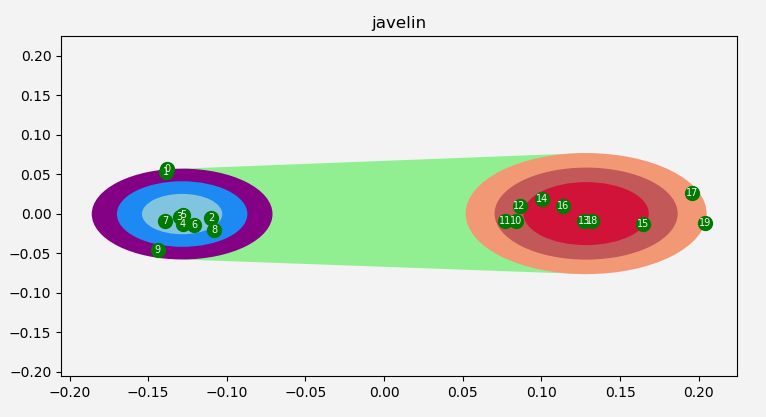
\includegraphics[width=\textwidth]{pictures/feedback_expert_cluster_example.png}
    \caption[Clusters formés par les données de l'expert]{Exemple de clusters formés à partir des données de l'expert (points verts). En bleu, le cluster des bons gestes, en rouge, le cluster des mauvais gestes pour le défaut appelé " Javelin ".}
    \label{fig:feedback_expert_cluster_example}
\end{figure}


Les limites de cette approche se situent dans l'impossibilité de corriger le problème si jamais deux clusters se superposent. La superposition des clusters implique que les différences entre les bons et mauvais gestes peuvent être plus ou moins floues, en fonction du degré de superposition. Cela implique que les données de l'expert ne sont pas suffisamment significatives par rapport au défaut observé, ou que les descripteurs observés ne sont pas significatifs par rapport au défaut. Une piste serait de vérifier la superposition ou non des deux clusters, et de supprimer automatiquement les points de données dont la distance au centroïde du cluster auquel ils sont assignés est la plus extrêmes, afin de réduire ou d'annuler la superposition des clusters.

Pour la visualisation des données de l'apprenant par rapport à celles de l'expert, une réduction de dimensionnalité des données est nécessaire lorsque celle-ci est supérieure à 2. Pour cette étape, une analyse en composantes principales (\textit{PCA}) est utilisé, afin d'obtenir la dimensionnalité voulue en sortie. Cette étape est réalisée juste avant l'affichage, afin d'effectuer tous les calculs sur les données non-modifiées. Un exemple de cet affichage est présent sur la Fig. \ref{fig:feedback_full_example}. On y voit un exemple avec quatre défauts identifiés, ainsi que les données de l'expert (cercles rouges et bleus). Cet affichage permet d'identifier dans quelle mesure le geste de l'apprenant correspond au geste cible : on remarque que pour les défauts " leaning " et " elbow move ", le centroïde de l'apprenant (en rouge) est compris dans le cluster des bons mouvements de l'expert. Par contre, pour les défauts " javelin " et " align arm ", les données de l'apprenant sont en moyenne plus proche du cluster de mauvais gestes. Ainsi, l'expert peut se baser sur ce retour visuel pour proposer des exercices permettant d'améliorer ces deux aspects du geste concernés.

Afin de proposer le(s) conseil(s) jugé(s) le(s) plus pertinent(s), le système doit être en mesure de fournir une indication quant à la présence plus ou moins forte des défauts identifiés. Pour répondre à ce besoin, une distance entre le centroïde des données de l'apprenant et les clusters expert est calculé. Soit $c_g$ le centroïde du clusters des bons gestes, $c_b$ le centroïde du clusters des mauvais gestes, et $c_a$ le centroïde des données de l'apprenant. On définit :
\[ A = y_{c_b} - y_{c_g} \]
\[ B = x_{c_b} - x_{c_g} \]
\[ C = (x_{c_g} * y_{c_b}) - (x_{c_b} * y_{c_g}) \]
La distance $D$ est défini comme il suit :
\[ D = \frac{A * x_{c_a}+ B * y_{c_a} + C}{\sqrt{A^2 + B^2}}\]

Cette distance correspond à la distance entre le centroïde des données de l'apprenant et le point de la droite reliant les centroïdes des deux clusters experts le plus proche. Elle se base sur l'hypothèse que si les données de l'apprenant se situent dans le trapézoïde (en vert sur les Fig. \ref{fig:feedback_full_example} et  \ref{fig:feedback_expert_cluster_example}) reliant les deux clusters de l'expert, le défaut est plus facilement corrigeable que s'il est en dehors de cette zone. Elle permet d'évaluer à quel point les descripteurs des données de l'apprenant sont éloignés de ceux de l'expert : plus elle est grande, plus l'apprenant est loin du geste de l'expert pour un défaut donné. Selon les cas d'utilisations, ce conseil peut être utilisé tel quel, ou l'expert peut se baser sur (i) la visualisation proposée par le système et/ou (ii) les conseils fournis par le système. Dans l'exemple montré dans la Figure \ref{fig:feedback_full_example}, on peut noter que le centroïde de l'apprenant, pour le défaut « \textit{align arm} », est situé en dehors des clusters et de l'espace situé entre ces clusters. Dans ce cas de figure, l'explication de cette distance peut être problématique. En effet, si les centroïde se situe dans l'alignement des clusters, bien qu'il soit en dehors des clusters et de la zone située entre eux, on peut supposer que le défaut est encore plus accentué chez l'apprenant. Cependant, lorsque le centroïde ne se situe pas dans cet alignement, il nous est pour l'instant impossible de donner une indication précise sur la nature du défaut de l'apprenant seulement à partir des données de mouvement ; ce point devra être travaillé dans le futur. Une piste serait de comparer la distance entre chaque descripteur extrait, afin de donner un retour sur l'aspect du geste étant le plus mauvais.
\afterpage{
\begin{landscape}
\begin{figure}
	\centering
    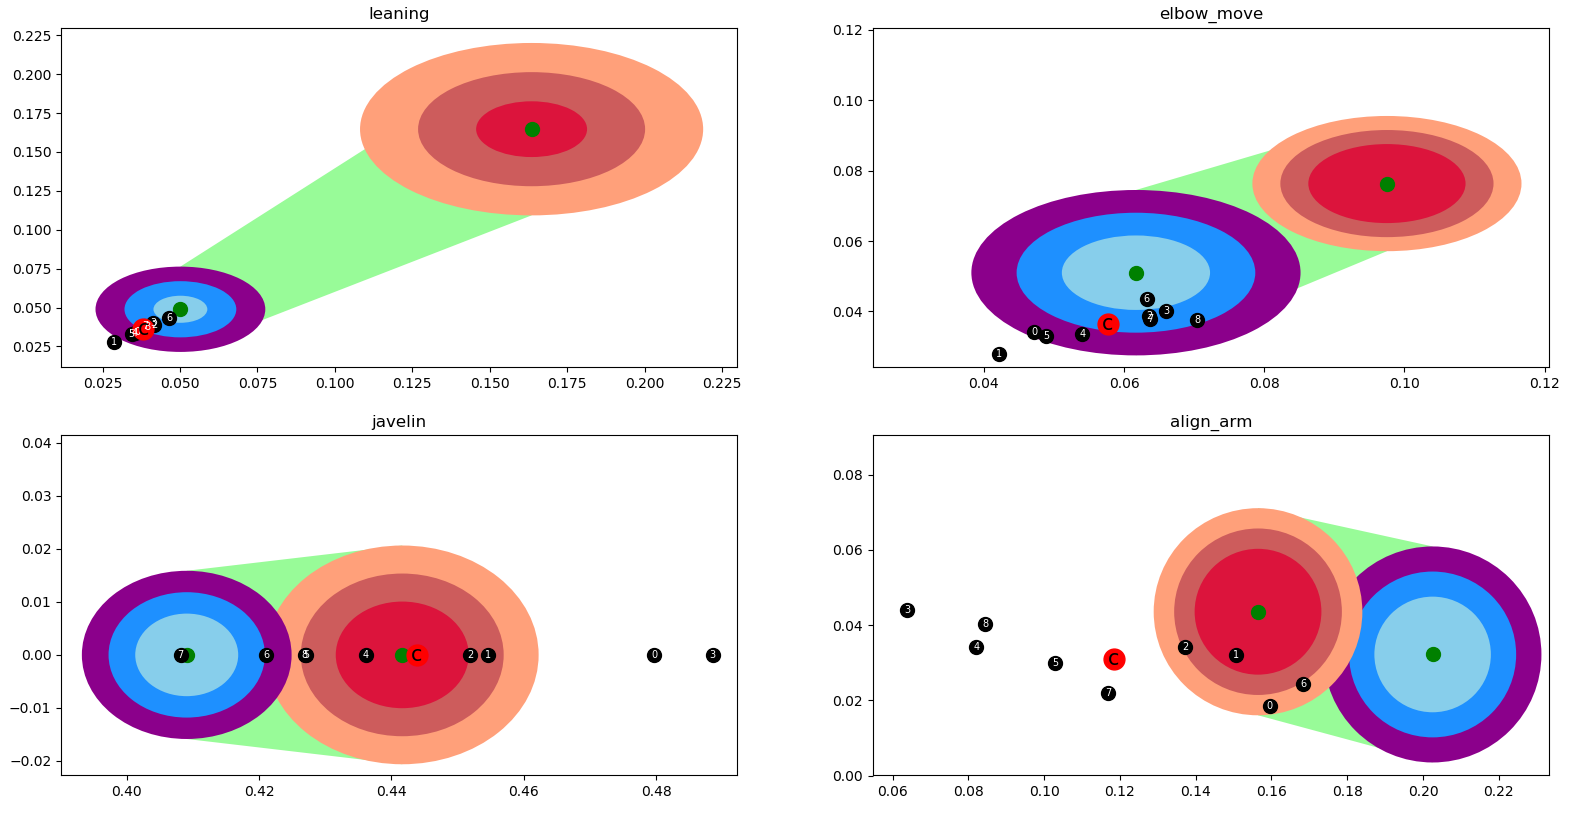
\includegraphics[width=23cm]{pictures/feedback_full_example.png}
    \caption[Feedback visuel proposé à l'expert]{Exemple de feedback visuel proposé à l'expert. Pour chaque défaut identifié (4 dans le cas présent), une visualisation des données de l'apprenant (points noirs) ainsi que du centroïde correspondant (points rouges) est affiché, afin de visualiser la distance de ces derniers par rapport aux données de l'expert pour un défaut identifié.}
    \label{fig:feedback_full_example}
\end{figure}
\end{landscape}}

\section{Résumé des contributions}
Dans cette partie, une chaine de traitement adaptée au Perception Neuron, pour l'analyse du mouvement capturé en situation d'apprentissage a été présentée. Les problèmes auxquels cette chaine de traitement propose des réponses sont (i) la modification de la taille des membres au cours du mouvement, (ii) les incohérences de positions des capteurs entre certaines frames. Plusieurs étapes de filtrage des données ont été présentées afin de palier ces problèmes. L'incohérence de positions des capteurs se traduisait par la présence de pics lors de l'extraction des vitesses. Ces pics ne correspondaient pas à la réalité du geste. Un filtre passe-bas a été appliqué, afin de compenser les artefacts du signal. Le problème de cette méthode est que les paramètres du filtre doivent être estimés (soit empiriquement, soit automatiquement) pour chaque signal, en fonction de ses caractéristiques propres, afin de ne pas trop " lisser " les valeurs réelles du signal.

Afin de ne garder que la partie utile du mouvement, un algorithme de segmentation a été présenté. L'algorithme de segmentation du mouvement utile permet de ne garder que les parties voulues du mouvement. Cet algorithme se base sur le maximum de la vitesse d'une articulation possédant les amplitudes et/ou variations du mouvement les plus importants, puis recherche un nombre prédéfini de minimums locaux les plus proches (à gauche et à droite). Il est possible de choisir le nombre de minimums locaux désirés, afin de garder une plus ou moins grande partie du signal original. Les limitations de cet algorithme se trouvent dans le postulat que le mouvement d'intérêt présente la vitesse la plus élevée.

Cette chaîne de traitement possède l'avantage d'être peu consommatrice de ressources dans le traitement des mouvements par rapport aux méthodes de la littérature, ce qui permet une utilisation en direct sur le terrain. En effet, le temps moyen de traitement d'un mouvement (allant du filtrage à l'extraction de données) est de cinq secondes. Cette étape de filtrage des données est cruciale, afin de pouvoir extraire des informations du mouvement qui seront cohérentes avec la réalité du geste.

Le système de retour à l'apprenant proposé dans cette partie permet d'obtenir une information visuelle de la performance de l'apprenant, par rapport à l'expert. À partir de données d'expert, contenant des bons mouvements et des mouvements présentant des défauts, et des données de l'apprenant, un affichage graphique permet de visualiser les différences entre le geste de l'expert et celui de l'apprenant. L'expert peut ensuite se baser sur ce retour afin d'ajuster ou non son jugement. Ce système permet d'analyser des modalités du gestes qui ne serait pas possible d'observer en temps normal, par exemple de par la nécessité d'observer trop de parties du corps à la fois, ou par l'occlusion de parties du corps résultant du mouvement lui-même.

Ce système a fait l'objet de plusieurs expérimentations, afin de vérifier son bon fonctionnement et sa capacité à fournir un retour à l'expert et à l'apprenant. Le prochain chapitre est consacré à ces expérimentations.

\chapter{Expérimentations}\label{chap:expe}
La chaîne de traitement précédemment présentée a pu être évaluée au travers de trois expérimentations : une première sur le lancer de balles dans une corbeille, une deuxième sur le \textit{Bottle Flip Challenge}, et une sur le lancer de fléchettes. Chaque expérimentation a pour but de tester une partie du système, cherchant à répondre aux hypothèses précédemment formulées :

\begin{itemize}
	\item \textbf{H1} : Il est possible de regrouper les gestes selon leurs propriétés cinématiques communes.
	\item \textbf{H2} : Il est possible de séparer les gestes des apprenants en deux groupes correspondant à une dichotomie geste réussi / geste raté afin de déterminer, pour une situation d'apprentissage donnée, les propriétés d'un ensemble fini de gestes réussis.
	\item \textbf{H3} : Il est possible de séparer les gestes en fonction de propriétés attendues et identifiées au préalable par l'expert.
	\item \textbf{H4} : Il est possible de corriger chaque défaut du geste de l'apprenant, en lui indiquant les défauts majeurs à corriger en premier. Un défaut majeur est identifié par la plus grande distance séparant le mouvement courant de l'apprenant, du groupe de gestes acceptables ayant éliminé ce défaut.
	\item \textbf{H5} : L'utilisation du système MLA basée sur l'hypothèse 4 permet d'améliorer l'apprentissage du geste par rapport à une situation sans le système MLA.
	\item \textbf{H6} : L'utilisation du système MLA en tant qu'assistant à l'enseignant permet d'améliorer l'apprentissage du geste par rapport à une situation sans MLA, et à une situation avec MLA et sans enseignant.
\end{itemize}

Ainsi, chaque expérimentation a pour objectif de répondre à une ou plusieurs de ces hypothèses :
\begin{itemize}
	\item Lancer de balles : \textbf{H1}, \textbf{H2}
	\item Bottle Flip Challenge : \textbf{H2}
	\item Lancer de fléchettes : \textbf{H3}, \textbf{H4}, \textbf{H5}, \textbf{H6}
\end{itemize}

\section{Lancer de balles dans une corbeille}
\subsection{Motivations et objectifs}
Afin de vérifier si le système est capable de séparer les gestes selon un étiquetage vérifiable par un humain à l'aide des descripteurs et des algorithmes choisis, une première expérimentation a été réalisée. Les hypothèses correspondantes sont les suivantes :
\begin{itemize}
    \item \textbf{H1} : Il est possible de regrouper les gestes selon leurs propriétés cinématiques communes.
	\item \textbf{H2} : Il est possible de séparer les gestes des apprenants en deux groupes correspondant à une dichotomie geste réussi / geste raté afin de déterminer, pour une situation d'apprentissage donnée, les propriétés d'un ensemble fini de gestes réussis.
\end{itemize}

Dans cette expérimentation, les personnes doivent lancer une balle dans une corbeille parmi deux disposées devant eux en ligne : l'une est située à 2 mètres devant la personne, et l'autre est située à 3.5 mètres devant la personne (Fig. \ref{fig:throwing_diagram}). Trois étiquetages différents ont été établis pour les lancers dans ce contexte :

\begin{enumerate}[label=(\roman*)]
	\item le degré de réussite (balle dans la corbeille ou non)
	\item la corbeille visée
	\item le type de lancer (lancer par le haut ou par le bas)
\end{enumerate}

Concernant les différents types de lancers, seuls deux types différents ont été réalisés par les personnes : le lancer « par le haut » et le lancer « par le bas ». Un geste de lancer « par le haut » est caractérisé par un mouvement de la main allant du haut vers le bas (trajectoire de la balle rectiligne ou légèrement courbée), alors qu'un geste de lancer « par le bas » est caractérisé par un mouvement de la main allant du bas vers le haut (trajectoire en cloche de la balle).

\begin{figure}
	\centering
    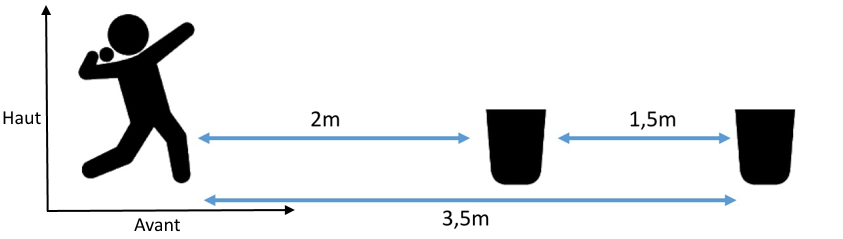
\includegraphics[width=\textwidth]{pictures/ball_throwing.png}
    \caption{Schéma de l'expérimentation du lancer de balle.}
    \label{fig:throwing_diagram}
\end{figure}

\subsection{Protocole}
Des instructions orales sont données quant à la tâche à effectuer : « Votre objectif est de lancer la balle dans une des deux corbeilles. Les cinquante premiers lancers devront viser la corbeille la plus proche, les cinquante autres la corbeille la plus éloignée. Vous êtes libre de lancer comme vous le souhaitez ». La personne retire ensuite tous les objets métalliques présents sur elle (ceinture, bracelets, téléphones, boucles d'oreilles, montres, etc.) afin d'éviter toute perturbation des capteurs (composés d'accéléromètres, de gyroscopes et de magnétomètres).

Le participant est ensuite mesuré selon les préconisations de NOITOM, afin de créer un squelette adapté selon douze mesures de distance suivantes :
\begin{itemize}
	\item Sommet du crâne jusqu'à la base du lobe de l'oreille / lèvre supérieure
	\item Base du lobe de l'oreille / lèvre supérieure jusqu'à la vertèbre C7
	\item Vertèbre C7 jusqu'au haut du fémur
	\item Largeur des épaules (épaule complète)
	\item Épaules (centre de rotation) jusqu'au coude (centre de rotation)
	\item Coude (centre de rotation) jusqu'au poignet (centre de rotation)
	\item Poignet (centre de rotation) jusqu'au bout du majeur
	\item Largeur des hanches (du fémur gauche jusqu'au fémur droit)
	\item Fémur jusqu'au genou (centre de rotation)
	\item Genou (centre de rotation) jusqu'à la cheville
	\item Cheville jusqu'au sol
	\item Talon jusqu'au bout du gros orteil
\end{itemize}

Une fois le squelette créé, les capteurs sont posés sur la personne. Le sujet se familiarise ensuite avec l'équipement, notamment en se déplaçant, afin de vérifier que la combinaison n'entrave pas ses mouvements. Cinq lancers sont ensuite réalisés avant le début de l'expérimentation, afin de se préparer et de s'habituer à l'équipement.

La combinaison est utilisée dans son intégralité, à l'exception des capteurs spécifiques aux doigts. En effet, nous avons constaté que l'utilisation de ces capteurs génère beaucoup de bruit dans les données de mouvement capturées, et ils ne sont pas nécessaires pour l'analyse réalisée.

Les calibrations sont ensuite effectuées afin d'étalonner les capteurs (position dans l'espace, espacement des capteurs entre eux, mise à zéro sur le logiciel de capture, etc.) pour que le logiciel puisse adapter la combinaison par rapport aux articulations du squelette 3D.

À chaque personne, il a été demandé de réaliser 100 lancers au total. Les 50 premiers lancers devaient viser la première corbeille, et les 50 autres devaient viser la seconde.

Une fois les lancers réalisés, l'export de chaque lancer au format BVH a été effectué. L'intervention humaine se borne à désigner le dossier contenant tous les fichiers de mouvements bruts. En premier lieu, les filtres sont appliqués. L'extraction des descripteurs fait suite à cette étape. La durée du chargement des fichiers BVH, le filtrage des descripteurs, l'extraction des descripteurs utilisés dans l'expérimentation et leur sauvegarde était d'environ 2 secondes par fichier sur une machine équipée d'un processeur 8 coeurs Intel Core i7-4910MQ 2.90GHz, 32Go de mémoire RAM tournant sous Windows 7.

Afin de vérifier la qualité du clustering, plusieurs métriques ont été utilisées en suivant principalement deux objectifs :
\begin{itemize}[label=$-$]
	\item évaluation interne des clusters, en assignant un score de vraisemblance pour chaque cluster, vérifiant la forme des clusters, leur cohésion, leur variance, etc.
	\item  évaluation externe des clusters, comparés les uns par rapport aux autres grâce à la distance les séparant, à l'aide d'une vérité terrain ou même d'une analyse experte \parencite{Jain1988ACD, Maulik2002Peo}
\end{itemize}

Afin de vérifier la séparabilité des données, la métrique utilisée est celle de l'Average Silhouette Score (\textit{ASS}) \parencite{Rousseeuw1987Sag}. Cette métrique se base sur le Silhouette Score (\textit{SS}) de chaque point individuel de donnée.

Soit $a(i)$ la distance moyenne d'un point $i$ par rapport à tous les autres points contenus dans le même cluster, définie par
\[a(i)={\frac {1}{|C_{i}|-1}}\sum _{j\in C_{i},i\neq j}d(i,j)\]
avec $d(i,j)$ la distance entre les points $i$ et $j$ au sein du cluster $C_i$. Cette mesure peut être considérée comme une indication de bonne appartenance du point $i$ au cluster $C_i$ : plus cette valeur est basse, plus le point $i$ est proche des autres points du cluster auquel il est assigné.

Soit $b(i)$ la distance moyenne minimale du point $i$ par rapport aux points des autres clusters (les distances moyennes étant calculées séparément pour chaque cluster ne contenant pas $i$), définie par
\[b(i)=\min _{k\neq i}{\frac {1}{|C_{k}|}}\sum _{j\in C_{k}}d(i,j)\]
avec $k$ étant le nombre de clusters.

Le Silhouette Score d'un point est défini par
\[s(i)={\frac {b(i)-a(i)}{\max\{a(i),b(i)\}}}, if |C_{i}|>1 |C_{i}|>1\]
et
\[s(i)=0, \text{si} |C_{i}|=1\]

L'Average Silhouette Score est la moyenne des Silhouette Scores de chaque échantillon du problème considéré. Ce score permet de mesurer dans quelle mesure l'échantillon appartient effectivement au cluster qui lui a été assigné, par rapport aux autres clusters. Cette valeur permet d'obtenir une estimation de l'homogénéité des clusters : une valeur élevée indique que les clusters sont bien séparés, alors qu'une valeur faible indique que les clusters sont proches, voire se superposent. Cette valeur varie entre -1 et 1 : une valeur de 1 signifie que tous les échantillons d'un cluster sont proches les uns des autres (les clusters sont bien séparés), alors qu'une valeur de 0 signifie que les clusters sont superposés. Dans ce dernier cas, une explication possible réside dans le nombre trop élevé ou trop faible de clusters. Struyf \textit{et al.} \parencite{Struyf1997Cia} ont proposé quatre paliers pour les valeurs de l'\textit{ASS} :
\begin{itemize}
	\item entre 0 et 0.25, aucune structure n'est discernable au sein des données
	\item entre 0.25 et 0.50, il existe une structure, bien que mal définie, voire artificielle
	\item entre 0.50 et 0.70, une structure existe au sein des données (séparation correcte des clusters)
	\item au-delà de 0.70, une structure est clairement définie au sein des données (très bonne séparation des clusters)
\end{itemize}

Dans le contexte de l'expérimentation, cette métrique permet donc de vérifier si les données sont séparables selon les descripteurs choisis.

S'il y a une séparation acceptable, il est nécessaire de déterminer les propriétés menant à cette séparation. Une approche consiste à corréler cette séparation avec le degré de réussite du geste. Dans le cas présent, ce degré est binaire : soit le geste est réussi (la balle a atterri dans la corbeille désignée), soit le geste est raté (la balle n'a pas atterri dans la corbeille désignée). En outre, il est aussi possible de considérer le type de lancer effectué ou la corbeille visée. Dans tous les cas, il faut disposer \textit{a priori} d'une vérité terrain, afin de pouvoir comparer le résultat du clustering à cet étiquetage. Dans ce contexte, plusieurs métriques ont été retenues : le rappel, la précision, le F1-score et l'Adjusted Rand Index (\textit{ARI}). Dans un problème de classification, le rappel indique la proportion d'éléments corrects contenus au sein de tous les éléments retournés, alors que la précision indique la proportion d'éléments corrects retournés par rapport au nombre d'éléments corrects total. Le F1-score correspond à la moyenne harmonique de ces deux valeurs. La valeur du F1 score se situe entre 0 et 1, avec une valeur de 1 indiquant une correspondance parfaite entre la séparation obtenue et la vérité terrain. Cependant, ce score n'est qu'une moyenne du F-score de chaque caractéristique de l'échantillon considéré. Ainsi, la valeur obtenue ne correspond pas au pouvoir discriminant des caractéristiques prises ensemble (information mutuelle) \parencite{Chen2006CSw}. %De plus, ce score donne une importance égale au rappel et à la précision ; en pratique, ce coût n'est pas toujours considéré comme égal \parencite{Hand2018Ano}.

L'\textit{ARI} est une mesure de similarité entre deux partitionnements de données différents \parencite{Morey1984ARI}. Cette mesure se base sur le Rand Index (RI) \parencite{Rand2971RI}. Soit un ensemble de $n$ données $E = {e_1, e_2, \ldots, e_n}$ et deux partitionnements de $E$ à comparer, avec $A = {A_1, \ldots, A_i}$ un partitionnement de $E$ en $i$ partitions et $B = {B_1, \ldots, B_j}$ un partitionnement de $E$ en $j$ partitions. On définit
\begin{itemize}
	\item $a$ comme étant le nombre de paires d'éléments dans $E$ qui se trouvent dans la même partition dans $A$ et dans $B$
	\item $b$ comme étant le nombre de paires d'éléments dans $E$ qui se trouvent dans des partitions différentes dans $A$ et dans $B$
	\item $c$ comme étant le nombre de paires d'éléments dans $E$ qui se trouvent dans la même partition dans $A$ et dans des partitions différentes dans $B$
	\item $d$ comme étant le nombre de paires d'éléments dans $E$ qui se trouvent dans des partitions différentes dans $A$ et dans la même partition dans $B$
\end{itemize}

Le Rand Index est défini par

\[ RI = \frac{a+b}{a+b+c+d} \]

Le dénominateur correspond au nombre total de paires d'éléments présents dans $E$. L'Adjusted Rand Index est une version normalisée du Rand Index \parencite{Hubert1985Cp}. Si on considère les mêmes éléments qu'auparavant (un ensemble de données $E$, et deux partitionnements $A$ et $B$), on peut créer un tableau de contingence comme suit :

\[
\begin{array}{c|cccc|c}
A \setminus B&B_{1}&B_{2}&\ldots &B_{j}&{\text{Sommes}}\\\hline
A_{1}&n_{11}&n_{12}&\ldots &n_{1l}&a_{1}\\
A_{2}&n_{21}&n_{22}&\ldots &n_{2l}&a_{2}\\
\vdots &\vdots &\vdots &\ddots &\vdots &\vdots \\
A_{i}&n_{i1}&n_{i2}&\ldots &n_{ij}&a_{j}\\\hline
{\text{Sommes}}&b_{1}&b_{2}&\ldots &b_{j}&
\end{array}
\]

Chaque case $n_{ij}$ indique le nombre d'éléments communs entre $A_i$ et $B_j$. L'Adjusted Rand Index est défini par la formule
\[ARI={\frac {\sum _{ij}{\binom {n_{ij}}{2}}-[\sum _{i}{\binom {a_{i}}{2}}\sum _{j}{\binom {b_{j}}{2}}]/{\binom {n}{2}}}{{\frac {1}{2}}[\sum _{i}{\binom {a_{i}}{2}}+\sum _{j}{\binom {b_{j}}{2}}]-[\sum _{i}{\binom {a_{i}}{2}}\sum _{j}{\binom {b_{j}}{2}}]/{\binom {n}{2}}}}\]

La valeur maximale est 1, et indique une correspondance parfaite entre les deux partitionnements de données. Une valeur de 0 correspond à une affectation aléatoire des données, et il est possible d'obtenir des valeurs négatives dans certains cas, dû à la normalisation \parencite{Meila2007Cca}.

Dans le contexte de l'expérimentation, ces métriques permettent de vérifier que le clustering obtenu correspond ou non à une séparation selon un étiquetage binaire.

\subsection{Données capturées}
Pour chaque lancer, le squelette de l'apprenant est capturé. Les mains sont représentées à l'aide d'un seul capteur. La réussite ou non du geste (la balle atterrit dans la corbeille désignée) est notée, ainsi que la corbeille visée et le type de lancer effectué.

\subsection{Données et métriques utilisées}
Pour chaque personne, 100 mouvements ont été enregistrés. Ces données sont enregistrées dans un format brut propriétaire de NOITOM (format RAW), puis exportées au format BVH (format ouvert d'animation de personnages, voir Chapitre \ref{chap:traitement_donnees}, section \ref{subsec:bvh}). Plusieurs descripteurs ont été extraits des mouvements, ayant chacun une valeur pour le début, la fin et l'indice de la valeur maximale de la vitesse moyenne de la main dominante :
\begin{itemize}
	\item la norme du vecteur vitesse (SN),
	\item la norme du vecteur vitesse en X, Y, Z (S x/y/z),
	\item la direction du vecteur vitesse en X, Y, Z (Sd x/y/z),
	\item la norme du vecteur vitesse ainsi que la direction de ce vecteur en X, Y, Z (SNDxyz).
\end{itemize}

L'utilisation des descripteurs liés à la vitesse se base sur l'hypothèse que la vitesse à imprimer à la balle afin de correctement viser la corbeille désignée serait différent selon la corbeille choisie. De plus, viser la corbeille la plus éloignée nécessite une force plus élevée, comparativement à la corbeille la plus proche. Enfin, les principales différences entre les types de lancers observés se situent au niveau de la direction de la balle, sa trajectoire ainsi que la force appliquée.

Plusieurs articulations ont été utilisées (alignée avec la préférence manuelle de la personne, gaucher ou droitier), correspondant aux parties du corps sollicitées lors du mouvement :
\begin{itemize}
	\item la main,
	\item l'avant-bras,
	\item le bras,
	\item l'épaule.
\end{itemize}
L'utilisation de plusieurs articulations permet de vérifier s'il existe d'une part une ou des articulations plus importantes pour la lancer, et d'autre part si la combinaison de descripteurs vitesses issus de plusieurs articulations permet d'augmenter la précision du clustering.

\subsection{Résultats}
Les résultats obtenus sont ceux d'une seule personne (100 lancers). L'utilisation de données de mouvement provenant d'une seule personne permet de limiter la variabilité des gestes de lancers : une fois un geste permettant de correctement viser la corbeille trouvé, les lancers suivants essayeront de reproduire les propriétés de ce lancer. Ainsi, on peut s'attendre à des données rapprochées (au sens des caractéristiques extraites) pour les lancers concernant une même corbeille. Le tableau \ref{throwing_results} présente les métriques calculées sur les clustering obtenus. Dans le cas des métriques de comparaison à une vérité terrain, les résultats sont donnés pour un clustering avec nombre de clusters $k = 2$. Les résultats pour la métrique permettant de vérifier la séparation des clusters sont également donnés pour $k = 2$, car c'est la valeur de $k$ qui donne les meilleurs résultats (quand la valeur $k = 2$ ne donne pas le meilleur résultat pour l'\textit{ASS}, les variations de cette valeur sont de l'ordre du centième, quelle que soit la valeur de $k$).

\begin{landscape}
\begin{table}[]
\centering
\begin{tabular}{|l|l|l|l|l|l|l|l|l|l|l|l|l|l|l|l|}
\hline
Joints & \multicolumn{5}{c|}{H}            & \multicolumn{5}{c|}{H, FA}        & \multicolumn{5}{c|}{H, FA, A}     \\ \hline
Metric & ASS  & P    & R    & F1   & ARI   & ASS  & P    & R    & F1   & ARI   & ASS  & P    & R    & F1   & ARI   \\ \hline
       & \multicolumn{15}{c|}{All data (ground truth = success / fail)}                                              \\ \hline
SN     & \cellcolor{green!25} 0.59 & 0.51 & 0.89 & 0.64 & 0.01  & 0.60 & 0.50 & 0.86 & 0.63 & 0.00  & 0.60 & 0.50 & 0.86 & 0.63 & 0.00  \\ \hline
Sxyz   & \cellcolor{green!25} 0.56 & 0.48 & 0.89 & 0.62 & -0.01 & 0.54 & 0.48 & 0.89 & 0.62 & -0.01 & 0.54 & 0.48 & 0.89 & 0.62 & -0.01 \\ \hline
Sdxyz  & 0.23 & 0.41 & 0.25 & 0.31 & -0.01 & 0.23 & 0.54 & 0.77 & 0.64 & 0.04  & 0.24 & 0.55 & 0.77 & 0.64 & 0.05  \\ \hline
SNDxyz & 0.26 & 0.53 & 0.89 & 0.67 & 0.04  & 0.27 & 0.55 & 0.77 & 0.64 & 0.05  & 0.26 & 0.53 & 0.77 & 0.63 & 0.03  \\ \hline
       & \multicolumn{15}{c|}{All data (ground truth = closest / farthest bin)}                                     \\ \hline
SN     & \cellcolor{green!25} 0.59 & 0.65 & 1.00 & 0.79 & 0.21  & 0.60 & 0.64 & 0.98 & 0.78 & 0.19  & 0.60 & 0.64 & 0.98 & 0.78 & 0.19  \\ \hline
Sxyz   & \cellcolor{green!25} 0.56 & 0.54 & 0.88 & 0.67 & 0.01  & 0.54 & 0.54 & 0.88 & 0.67 & 0.01  & 0.54 & 0.54 & 0.88 & 0.67 & 0.01  \\ \hline
Sdxyz  & 0.23 & 0.65 & 0.34 & 0.45 & 0.02  & 0.23 & 0.68 & 0.86 & 0.76 & 0.20  & 0.24 & 0.69 & 0.86 & 0.77 & 0.22  \\ \hline
SNDxyz & 0.26 & 0.68 & 0.98 & 0.80 & 0.26  & 0.27 & 0.71 & 0.88 & 0.79 & 0.26  & 0.26 & 0.69 & 0.88 & 0.77 & 0.22  \\ \hline
       & \multicolumn{15}{c|}{All data (ground truth = throwing type)}                                              \\ \hline
SN     & \cellcolor{green!25} 0.59 & 0.87 & 0.95 & 0.91 & \textbf{0.83}  & 0.60 & 0.83 & 0.95 & 0.89 & 0.79  & 0.60 & 0.83 & 0.95 & 0.89 & 0.79  \\ \hline
Sxyz   & \cellcolor{green!25} 0.56 & 0.06 & 0.05 & 0.05 & -0.09 & 0.54 & 0.06 & 0.05 & 0.05 & -0.09 & 0.54 & 0.06 & 0.05 & 0.05 & -0.09 \\ \hline
Sdxyz  & 0.23 & 0.08 & 0.10 & 0.09 & -0.07 & 0.23 & 0.54 & 0.95 & 0.69 & 0.39  & 0.24 & 0.53 & 0.95 & 0.68 & 0.37  \\ \hline
SNDxyz & 0.26 & 0.74 & 0.95 & 0.83 & 0.68  & 0.27 & 0.55 & 1.00 & 0.71 & 0.42  & 0.26 & 0.56 & 0.95 & 0.70 & 0.42  \\ \hline
\end{tabular}
\caption{Métriques calculées sur les résultats du clustering pour le lancer de balle.}
\label{throwing_results}
\end{table}
\end{landscape}

L'ajout d'articulations n'améliore pas (ou de manière marginale) la séparation des clusters dans tous les cas (valeurs d'$ASS$ et d'$ARI$ stables ou diminuant lors d'ajout d'autres articulations). Cela montre que la main reste l'articulation la plus discriminante pour la séparation des gestes. Dans le cas de la réussite ou non du geste, bien qu'une séparation acceptable soit possible à l'aide de la norme du vecteur vitesse ($ASS \approx 0.60$ pour les meilleurs cas), ainsi que les vecteurs vitesses en x, y et z, cette séparation ne correspondait pas au degré de réussite du geste ($ARI \approx 0$).

Pour la corbeille ciblée, les mêmes tendances se dégagent pour la séparation des clusters. Cette fois, l'\textit{ARI} obtient des valeurs $\approx 0.25$, suggérant une légère correspondance des regroupements avec l'étiquetage. Cependant, les valeurs d'\textit{ASS} correspondantes sont aux alentours de $0.25$, suggérant une mauvaise séparation des clusters.

Il est intéressant de noter qu'il a été possible d'obtenir à la fois une valeur correcte pour l'\textit{ASS} (0.59) et une valeur élevée pour l'\textit{ARI} (0.83) pour la séparation par rapport au type de lancer, avec le descripteur de la norme du vecteur vitesse. Cette corrélation entre une bonne valeur pour l'\textit{ASS} et une forte valeur pour l'\textit{ARI} suggère qu'il est possible, à l'aide des descripteurs et des méthodes utilisées, de séparer les gestes selon un critère observable par un humain. Ainsi, l'hypothèse \textbf{H1} a été validée dans le contexte de cette expérimentation. Cependant, cette séparation n'est pas corrélée avec le degré de réussite du geste, et l'hypothèse \textbf{H2} n'a pas pu être validée au cours de cette expérimentation. Une autre expérimentation a été conduite, afin de se focaliser sur la séparation du geste en fonction du résultat obtenu.

\section{Bottle Flip Challenge}
Le Bottle Flip Challenge est un défi qui provient de la performance d'un étudiant lors d'un concours de talents américain, au sein du lycée Ardrey Kell \parencite{BottleFlipChallengeOrigin}. L'étudiant de 18 ans, Mike Senatore, a offert au public une performance inattendue : un lancer de bouteille, partiellement remplie, qui réalise un salto arrière, avant de retomber parfaitement droite, sur la table (Fig. \ref{fig:BFC_example}). Filmé à l'aide d'un smartphone, la vidéo se propage rapidement sur internet, et de nombreuses personnes s'y essayent : le \textit{Bottle Flip Challenge} était né.

Ce mouvement possède l'avantage de ne nécessiter que peu de matériel : une bouteille d'eau partiellement remplie et une table. La durée du mouvement est également très courte, ce qui permet d'enregistrer beaucoup de données en un temps réduit. De plus, le geste ne nécessite pas de connaissance \textit{a priori}, ce qui fait qu'il n'est pas nécessaire d'avoir à disposition des personnes ayant déjà réalisé ce geste.

\begin{figure}
	\centering
    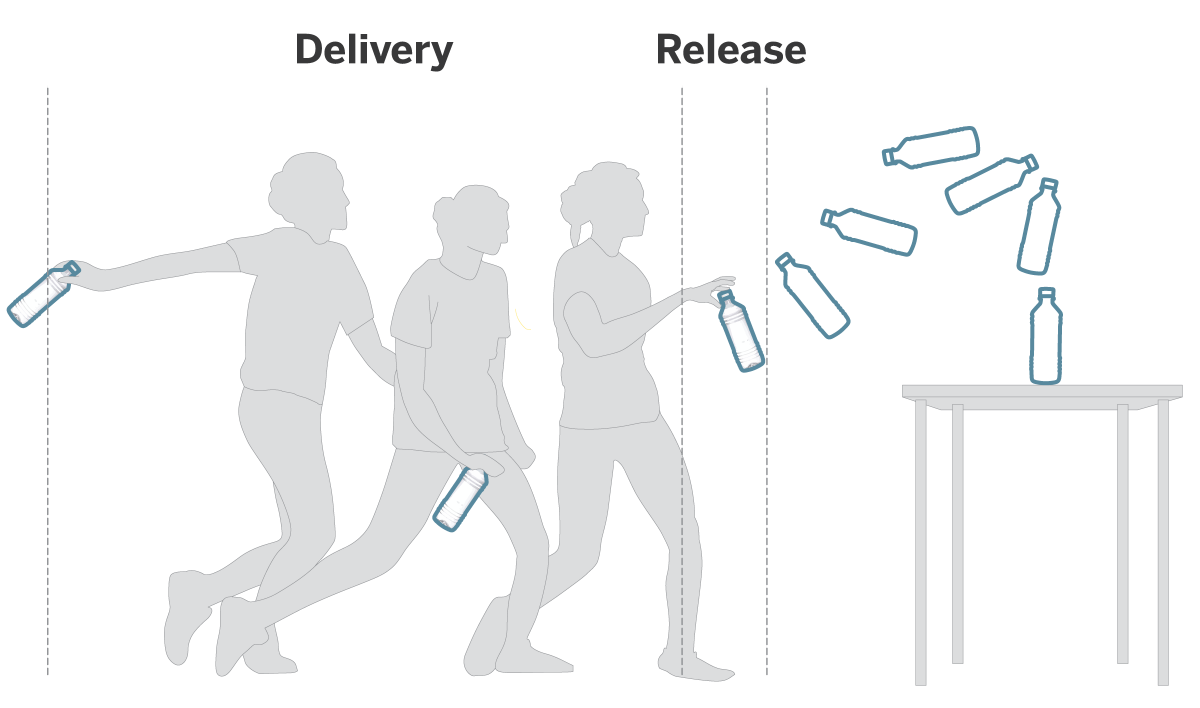
\includegraphics[width=\textwidth]{pictures/BFC_example.png}
    \caption[Exemple du mouvement du Bottle Flip Challenge]{Exemple du mouvement du Bottle Flip Challenge \protect\footnotemark.}
    \label{fig:BFC_example}
\end{figure}


Le mouvement de la bouteille, ainsi que de l'eau au sein de la bouteille, ont fait l'objet d'une étude récente \parencite{Dekker2018BF}. Il en ressort que les phénomènes physiques les régissant sont complexes et nombreux : dynamique des fluides, mouvement du projectile, moment cinétique, force centripète et gravité. Il ressort de cette étude scientifique que le lancer optimal présente un centre d'inertie bas, une vitesse angulaire faible et que le taux de remplissage optimal pour la bouteille se situe entre $20$ et $40$ \% de sa capacité maximale. Une autre étude \parencite{BFCAnalysis} montre qu'une bonne manière de lancer pour le Bottle Flip Challenge est de ne donner qu'une faible impulsion vers l'avant, et de lâcher la bouteille lorsqu'elle se trouve perpendiculaire au sol.

\subsection{Motivations et objectifs}
L'objectif de cette expérimentation était de déterminer s'il était possible d'obtenir une séparation des données en deux clusters, correspondant au degré de réussite du geste. Pour que le geste soit considéré comme réussi, il faut que la bouteille soit debout, sur la table, après avoir réalisé une rotation. L'hypothèse correspondante est la suivante :

\begin{itemize}
	\item \textbf{H2} : Il est possible de séparer les gestes des apprenants en deux groupes correspondant à une dichotomie geste réussi / geste raté afin de déterminer, pour une situation d'apprentissage donnée, les propriétés d'un ensemble fini de gestes réussis.
\end{itemize}

\footnotetext{https://wadsworthbruin.com/2016/12/01/bottle-flipping-into-the-heart-of-wadsworth-high/}

\subsection{Protocole}
La personne participante doit remplir un pré-questionnaire, contenant des informations sur le nom, l'âge, la taille, les connaissances par rapport au Bottle Flip Challenge. Des instructions orales sont données : \linebreak
\og Le but de cette expérience est de lancer une bouteille, de manière à ce qu’elle fasse un tour sur son axe horizontal avant de retomber correctement sur la table. Vous êtes libre sur la position de votre corps et le geste de lancer. Cependant, voici le geste communément utilisé pour réussir le lancer [faire une démonstration]. Il vous est demandé de vous mettre droit, les pieds avant la marque au sol, les bras le long du corps, la bouteille tenue dans votre main. Lorsque le premier bip retentira, vous lancerez la bouteille. Une fois le lancer terminé, vous remettrez les bras le long du corps, et attendrez que le deuxième bip retentisse avant de la reprendre, puis de vous remettre en position. Je vous signalerai lorsque vous aurez réalisé suffisamment de lancers. \fg

La personne retire ensuite tous les objets métalliques présents sur elle (ceinture, bracelets, téléphones, boucles d'oreilles, montres, etc.).

La personne est mesurée selon les préconisations de NOITOM \parencite{Noitom2015Doc}, pour qu'un squelette adapté soit créé. Une fois le squelette créé, les capteurs sont posés sur la personne. Le sujet se familiarise ensuite avec l'équipement, notamment en se déplaçant, afin de vérifier que la combinaison n'entrave pas le mouvement. Cinq lancers sont ensuite réalisés avant le début de l'expérimentation, pour se préparer, s'habituer à l'équipement et vérifier que le gant de la combinaison ne gêne pas la prise de la bouteille. L'installation complète est visible sur la figure \ref{fig:BFC_diagram}.

\begin{figure}
	\centering
    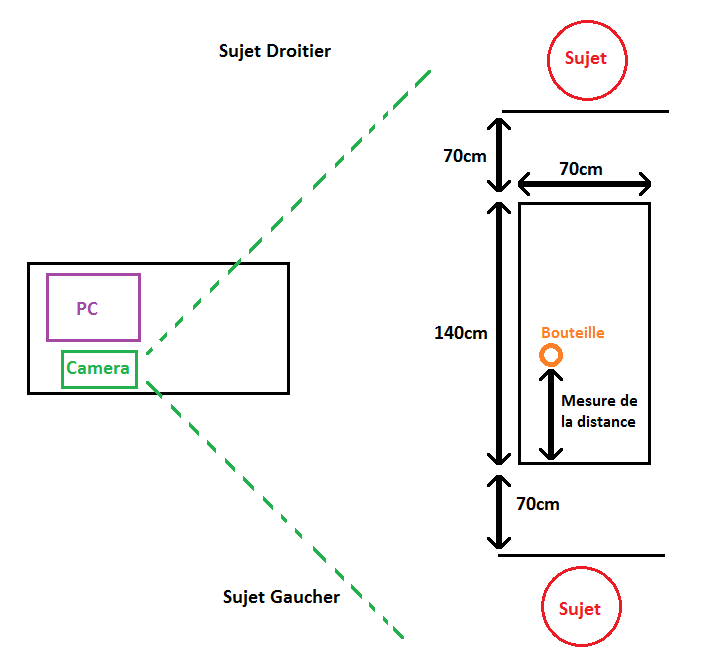
\includegraphics[width=\textwidth]{pictures/BFC_diagram.png}
    \caption{L'installation du matériel lors de l'expérimentation du Bottle Flip Challenge (vue du dessus).}
    \label{fig:BFC_diagram}
\end{figure}

Une fois les données de mouvement capturées, le même processus que pour la précédente expérimentation est utilisé afin d'importer, de filtrer, d'extraire les descripteurs et de sauvegarder les données ainsi extraites.

Les métriques utilisées pour analyser les résultats sont les mêmes que pour la précédente expérimentation.

\subsection{Données capturées}
Pour chaque lancer, le squelette de l'apprenant est capturé, y compris le mouvement des doigts. La réussite ou non du geste (bouteille qui atterrit correctement ou non après le salto arrière) est notée, et pour les gestes réussis, la distance de la bouteille par rapport au bord de la table où se situe la personne est mesurée.

\subsection{Données et métriques utilisées}
13 personnes au total ont participé à l'expérimentation. Pour chacune d'entre elles, 100 mouvements ont été enregistrés. Ces données sont enregistrées au format RAW de NOITOM, puis exportées dans le format BVH. Les mêmes descripteurs que précédemment ont été extraits, et les mêmes combinaisons d'articulations ont été utilisées.

L'hypothèse est que la vitesse de la bouteille est l'indicateur prédominant dans la réussite du geste : une vitesse trop faible ne permettrait pas à la bouteille de faire une rotation complète, et une vitesse trop élevée induirait plusieurs rotations, ainsi qu'un atterrissage non maîtrisé. La direction est utilisée afin de vérifier l'hypothèse que la direction du lancer influait également sur la réussite du geste.

\subsection{Résultats}
Dans le cas des métriques de comparaison à une vérité terrain, les résultats sont donnés pour un clustering avec nombre de clusters $k = 2$. Les résultats pour la métrique permettant de vérifier la séparation des clusters sont également donnés pour $k = 2$, car c'est la valeur de $k$ qui donne les meilleurs résultats (quand la valeur $k = 2$ ne donne pas le meilleur résultat pour l'\textit{ASS}, les variations de cette valeur sont de l'ordre du centième, quelle que soit la valeur de $k$). Lors de cette expérimentation, la combinaison de capteurs présentait beaucoup plus d'artefacts sur les articulations allant de l'épaule à la main sur le côté gauche. Les données des personnes gauchères présentaient donc plus de bruits que les données des personnes droitières. Ainsi, il a été décidé de faire les tests avec :

\begin{enumerate}[label=(\roman*)]
	\item les données mixtes (1300 données),
	\item les gauchers seuls (200 données),
	\item les droitiers seuls (1100 données).
\end{enumerate}

Les résultats sont présentés dans le tableau \ref{BfC_results}.

\begin{landscape}

\begin{table}[]
\centering
\begin{tabular}{|l|l|l|l|l|l|l|l|l|l|l|l|l|l|l|l|}
\hline
Joints & \multicolumn{5}{c|}{H}           & \multicolumn{5}{c|}{H,FA}        & \multicolumn{5}{c|}{H, FA, A}    \\ \hline
Metric & ASS  & P    & R    & F1   & ARI  & ASS  & P    & R    & F1   & ARI  & ASS  & P    & R    & F1   & ARI  \\ \hline
& \multicolumn{15}{|c|}{Left and Right-Handed}                                                                    \\ \hline
SN     & 0.48 & 0.25 & 0.33 & 0.29 & 0.04 & 0.44 & 0.25 & 0.33 & 0.29 & 0.04 & 0.43 & 0.25 & 0.33 & 0.29 & 0.04 \\ \hline
Sxyz   & \cellcolor{green!25} 0.54 & 0.18 & 0.67 & 0.30 & 0.05 & 0.52 & 0.27 & 0.32 & 0.29 & 0.05 & 0.51 & 0.18 & 0.68 & 0.29 & 0.05 \\ \hline
Sdxyz  & 0.24 & 0.21 & 0.53 & 0.30 & 0.00 & 0.27 & 0.25 & 0.25 & 0.25 & 0.04 & 0.22 & 0.18 & 0.72 & 0.27 & 0.04 \\ \hline
SNDxyz & 0.21 & 0.18 & 0.47 & 0.30 & 0.00 & 0.27 & 0.25 & 0.26 & 0.26 & 0.04 & 0.22 & 0.26 & 0.28 & 0.27 & 0.04 \\ \hline
& \multicolumn{15}{|c|}{Left Handed}                                                                              \\ \hline
SN     & 0.41 & 0.39 & 0.39 & 0.39 & 0.02 & 0.42 & 0.38 & 0.39 & 0.39 & 0.01 & 0.41 & 0.31 & 0.61 & 0.39 & 0.01 \\ \hline
Sxyz   & 0.35 & 0.32 & 0.57 & 0.39 & 0.00 & 0.34 & 0.32 & 0.57 & 0.39 & 0.00 & 0.33 & 0.35 & 0.43 & 0.39 & 0.00 \\ \hline
Sdxyz  & 0.31 & 0.34 & 0.48 & 0.40 & 0.00 & 0.27 & 0.34 & 0.54 & 0.39 & 0.00 & 0.23 & 0.34 & 0.48 & 0.40 & 0.00 \\ \hline
SNDxyz & 0.27 & 0.34 & 0.49 & 0.40 & 0.00 & 0.25 & 0.33 & 0.48 & 0.39 & 0.00 & 0.22 & 0.34 & 0.52 & 0.41 & 0.00 \\ \hline
& \multicolumn{15}{|c|}{Right Handed}                                                                             \\ \hline
SN     & 0.42 & 0.18 & 0.29 & 0.22 & 0.00 & 0.36 & 0.17 & 0.28 & 0.21 & 0.00 & 0.34 & 0.17 & 0.28 & 0.21 & 0.00 \\ \hline
Sxyz   & \cellcolor{green!25} 0.73 & 0.19 & 0.12 & 0.15 & 0.01 & 0.71 & 0.19 & 0.12 & 0.15 & 0.01 & 0.71 & 0.19 & 0.12 & 0.15 & 0.01 \\ \hline
Sdxyz  & 0.28 & 0.15 & 0.45 & 0.28 & 0.00 & 0.20 & 0.16 & 0.49 & 0.27 & 0.00 & 0.26 & 0.19 & 0.13 & 0.15 & 0.01 \\ \hline
SNDxyz & 0.26 & 0.16 & 0.45 & 0.28 & 0.00 & 0.19 & 0.19 & 0.52 & 0.27 & 0.00 & 0.26 & 0.17 & 0.87 & 0.15 & 0.01 \\ \hline
\end{tabular}
\caption{Métriques calculées sur les résultats du clustering pour le Bottle Flip Challenge.}
\label{BfC_results}
\end{table}
\end{landscape}

Dans tous les cas, l'ajout d'autres articulations que celle de la main ne fait que rajouter du bruit (les valeurs de l'$ASS$ et l'$ARI$ décroissent). Les plus fortes valeurs d'\textit{ASS} (séparation des clusters) ont été obtenues pour les descripteurs vecteur vitesse en X, Y, Z ($ASS$ des descripteurs Sxyz $= 0.73$). On peut également remarquer que les résultats de l'\textit{ASS} sont meilleurs sur les données des droitiers seuls pour ces descripteurs, par opposition aux données mixtes ou des gauchers seulement (dernière partie du tableau \ref{BfC_results}). Cette tendance tend à confirmer les problèmes de capteurs du côté gauche de la combinaison. Le tableau 7 montre que les valeurs les plus discriminantes pour la séparation sont le vecteur vitesse en Z (en avant) et en Y (en haut) au moment de la vitesse maximale. Cette séparation est cohérente avec les études réalisées par \parencite{Dekker2018BF} et \parencite{BFCAnalysis} qui suggèrent que les différences entre un lancer réussi et raté se situent au niveau de la force et de la direction du lancer.

\begin{table}[]
\centering
\begin{tabular}{|l|l|l|l|}
\hline
            & Beginning & Maximum & End    \\ \hline
X (Side)    & 0.0398    & 0.5071  & 0.0110 \\ \hline
Y (Upward)  & 0.0415    & \cellcolor{green!25} 1.7497  & 0.0998 \\ \hline
Z (Forward) & 0.0847    & \cellcolor{green!25} 2.0477  & 0.0536 \\ \hline
\end{tabular}
\label{BfC_best_descriptors}
\caption[Distance relative entre les centroïdes des clusters, pour la main droite, avec les vecteurs vitesse en X, Y, Z pour $k = 2$.]{Distance relative entre les centroïdes des clusters, pour la main droite, avec les vecteurs vitesse en X, Y, Z pris au début, au maximum et à la fin du lancer, pour $k = 2$.}
\end{table}

Dans tous les cas, les valeurs de l'\textit{ARI} (correspondance avec la vérité terrain) sont restées proches de 0, ce qui indique que les séparations obtenues ne correspondaient pas au degré de réussite du geste. Ainsi, l'hypothèse \textbf{H2} n'a pas été validée au cours de cette expérimentation.

Les descripteurs utilisés conjointement avec les algorithmes de clustering ne peuvent donc pas proposer un regroupement corrélé avec le degré de réussite du geste, dans le cas du \textit{Bottle Flip Challenge}. Le peu de variabilité du geste d'un lancer à un autre (et, par extension, d'un lancer réussi à un lancer raté) est une piste pour expliquer que l'algorithme des \textit{k-means} appliqué non récursivement n'est pas suffisant pour obtenir une telle séparation. De plus, les descripteurs utilisés dans cette expérimentation sont tous basés sur la vitesse. Ce type d'indicateurs semble ne pas être suffisant pour caractériser la réussite ou non du geste. Plusieurs autres descripteurs auraient pu être utilisés, tels que la courbure (indication sur la vitesse de changement d'une courbe au cours du temps), la vitesse angulaire des articulations sollicitées (poignet et main), ainsi que le déplacement du centre de masse de la personne, \textit{etc.} La complexité des phénomènes physiques régissant le lancer (autant pour le mouvement du bras et de la main que celui de l'eau dans la bouteille) peuvent également indiquer que les descripteurs basés vitesses ne sont pas suffisant pour caractériser tous les aspects du geste important pour un lancer réussi.

Plusieurs problèmes ont également émané de l'expérimentation elle-même. Premièrement, la distance entre la table et la personne lançant n'était pas systématiquement constante. En effet, certaines personnes prenaient un léger élan, ou se reculaient légèrement avant de lancer par rapport à la position limite imposée (voir figure \ref{fig:BFC_diagram}). De plus, il n'était pas possible de mesurer le point d'impact exact de la bouteille sur la table, car cette dernière glissait lors d'un lancer réussi. Cette distance n'a ainsi pas été considérée pour notre analyse. Bien que corrigée à l'aide de pré-traitements, l'imprécision des données de capture récoltées (cf. chapitre \ref{chap:traitement_donnees} section \ref{sec:traitements}) est également un facteur à prendre en compte dans les résultats obtenus.

\subsection{Discussion}
Ces deux premières expérimentations ont permis de vérifier la capacité de la plateforme MLA à traiter de manière automatique les données, une fois paramétrée selon les besoins d'analyse. Ces expérimentations ont également permis de vérifier s'il était possible d'obtenir automatiquement une séparation entre les gestes jugés réussis et ceux jugés ratés, pour un cas précis. Les descripteurs choisis, ainsi que la méthode utilisée, ont permis d'aboutir à une séparation des données acceptable dans les deux expérimentations.

Cependant, pour le \textit{Bottle Flip Challenge}, la séparation obtenue ne correspond pas à une dichotomie geste réussi/raté. Le manque d'analyse experte est un problème qui est apparu au cours de l'expérimentation. Bien que le Bottle Flip Challenge ait fait l'objet d'articles scientifiques sur la physique régissant le lancer et la bouteille \parencite{Dekker2018BF, BFCAnalysis}, il ne semble pas y avoir d'expertise formalisée du geste au moment où ces lignes sont écrites. En ce qui concerne l'étude du geste, la rotation du poignet aurait pu être une piste intéressante à explorer. Un sous-ensemble réduit de descripteurs a été utilisé pour cette expérimentation, ce qui a limité les résultats obtenus. Le calcul d'autres descripteurs (tels que ceux présentés dans \parencite{larboulette2015Descriptors} par exemple) aurait pu mener à de meilleurs résultats.

L'analyse du geste, dans le cas de ces deux expérimentations, se fait de manière binaire : soit le geste est acceptable, soit il ne l'est pas. Dans une situation d'apprentissage, il n'est pas toujours possible de regrouper ces mouvements dans ces deux catégories. Le degré de succès peut avoir une granularité plus fine, ou dépendre de l'acceptabilité binaire (ou non) de plusieurs autres propriétés du geste.

De plus, dans un tel processus, l'humain est écarté du processus d'analyse. Son expertise n'est utilisée qu'\textit{a priori}, et son intervention n'est pas requise dans le processus d'évaluation et \textit{in fine} de conseil pour l'apprentissage. Bien qu'un tel système puisse présenter des avantages, l'objectif est de proposer une aide à la décision pour l'enseignant/l'expert, et non pas un remplacement de ce dernier. Le système de retours de MLA, basé sur une analyse et une évaluation par regroupement des besoins d'observation du geste, permet de fournir un retour graphique à l'expert ou à l'apprenant. Ce système est l'objet de l'expérimentation suivante.

\section{Expérimentation : lancer de fléchettes}
Cette section présente l'évaluation de la partie de retours à l'apprenant du système MLA au travers d'une expérimentation portant sur le lancer de fléchettes. Il s'agit d'un sport où la technicité du geste est formalisée \footnote{\url{https://www.dartslive.com/enjoy/en/throw/}}. Il existe, pour chaque partie du corps impliquée, des explications précises quant à la position et au mouvement. Après une analyse de ces explications, nous proposons une représentation du geste sous la forme d'un ensemble de descripteurs représentant chaque besoin d'observation. Les valeurs d'acceptabilité de ces descripteurs sont ensuite estimées à l'aide d'un clustering basé sur les démonstrations de l'expert. Enfin, ces valeurs sont comparées à celles de l'apprenant afin de lui fournir un retour.

\subsection{Motivations et objectifs}
Les objectifs de cette expérimentation sont multiples. Il s'agit d'une part de montrer qu'il est possible, à l'aide du système de retours à l'apprenant basé sur les démonstrations de l'expert et l'estimation de valeurs d'acceptabilité empiriques des propriétés du geste, de donner des conseils pertinents lors de la réalisation de ces derniers. D'autre part, il s'agit également de montrer qu'une amélioration du geste, en termes de précision du tir et de la « forme » du mouvement résultait de ces conseils. Enfin, l'efficacité du système selon les modalités précédemment citées est évaluée en termes d'usage : utilisation du système seul, ou utilisation conjointe avec l'analyse de l'expert.

Les hypothèses correspondantes sont les suivantes :
\begin{itemize}
    \item \textbf{H3} : Il est possible de séparer les gestes en fonction de propriétés attendues et identifiées au préalable par l'expert.
	\item \textbf{H4} : Il est possible de corriger chaque défaut du geste de l'apprenant, en lui indiquant les défauts majeurs à corriger en premier. Un défaut majeur est identifié par la plus grande distance séparant le mouvement courant de l'apprenant, du groupe de gestes acceptables ayant éliminé ce défaut.
	\item \textbf{H5} : L'utilisation du système MLA basée sur l'hypothèse 4 permet d'améliorer l'apprentissage du geste par rapport à une situation sans le système MLA.
	\item \textbf{H6} : L'utilisation du système MLA en tant qu'assistant à l'enseignant permet d'améliorer l'apprentissage du geste par rapport à une situation sans MLA, et à une situation avec MLA et sans enseignant.
\end{itemize}


En conséquence, l'objectif pour les personnes réalisant l'expérimentation est de viser le centre de la cible, et également de suivre les conseils donnés par l'expert utilisant le système ou non.

Afin d'évaluer les résultats obtenus, trois groupes ont été formés : un groupe " contrôle ", où seul l'expert donne des conseils (système absent), un groupe où seul le système donne les conseils (évaluation experte absente), et un groupe où l'expert peut s'appuyer sur le système afin de décider des conseils à donner.

\subsection{Fléchettes : principes et description}
\subsubsection{Matériel}
Le lancer de fléchettes est un sport qui se pratique à l'aide d'une cible (Figures \ref{fig:darts_target} et \ref{fig:darts_zone}) et de fléchettes (Fig. \ref{fig:single_dart}). La cible est constituée de vingt zones distinctes et de tailles égales, numérotées de 1 à 20, ainsi que d'un cercle au centre (Fig. \ref{fig:darts_target}). Chacune des zones est également divisée (Fig. \ref{fig:darts_zone}) :

\begin{itemize}
	\item les simples sont les deux plus grandes parties d'une zone,
	\item les doubles se situent sur la couronne extérieure des zones,
	\item les triples se situent sur la couronne intérieure des zones.
\end{itemize}

Le double centre compte comme un " double " du centre simple ($2 \times 25$).

\begin{figure}
    \centering
    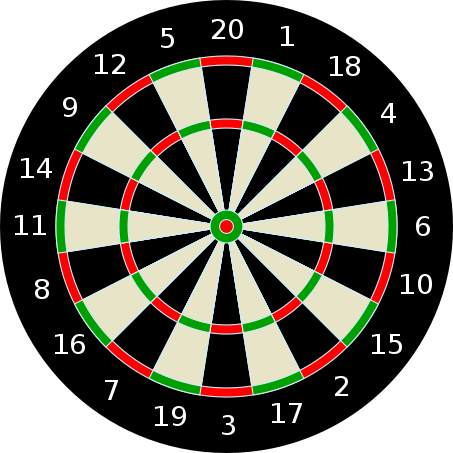
\includegraphics[width=5cm]{pictures/darts_target.png}
    \caption[Cible de fléchettes]{Une cible de fléchettes classique$^1$.}
    \label{fig:darts_target}
\end{figure}

\begin{figure}
    \centering
    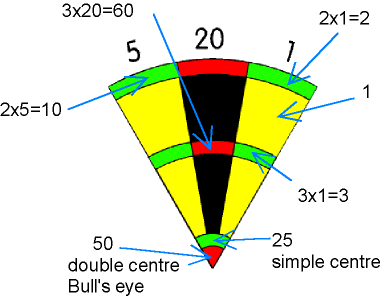
\includegraphics[width=5cm]{pictures/darts_zone.png}
    \caption[Zones d'une cible de fléchettes]{Détail des zones d'une cible de fléchettes classique$^1$.}
    \label{fig:darts_zone}
\end{figure}

\begin{figure}
    \centering
    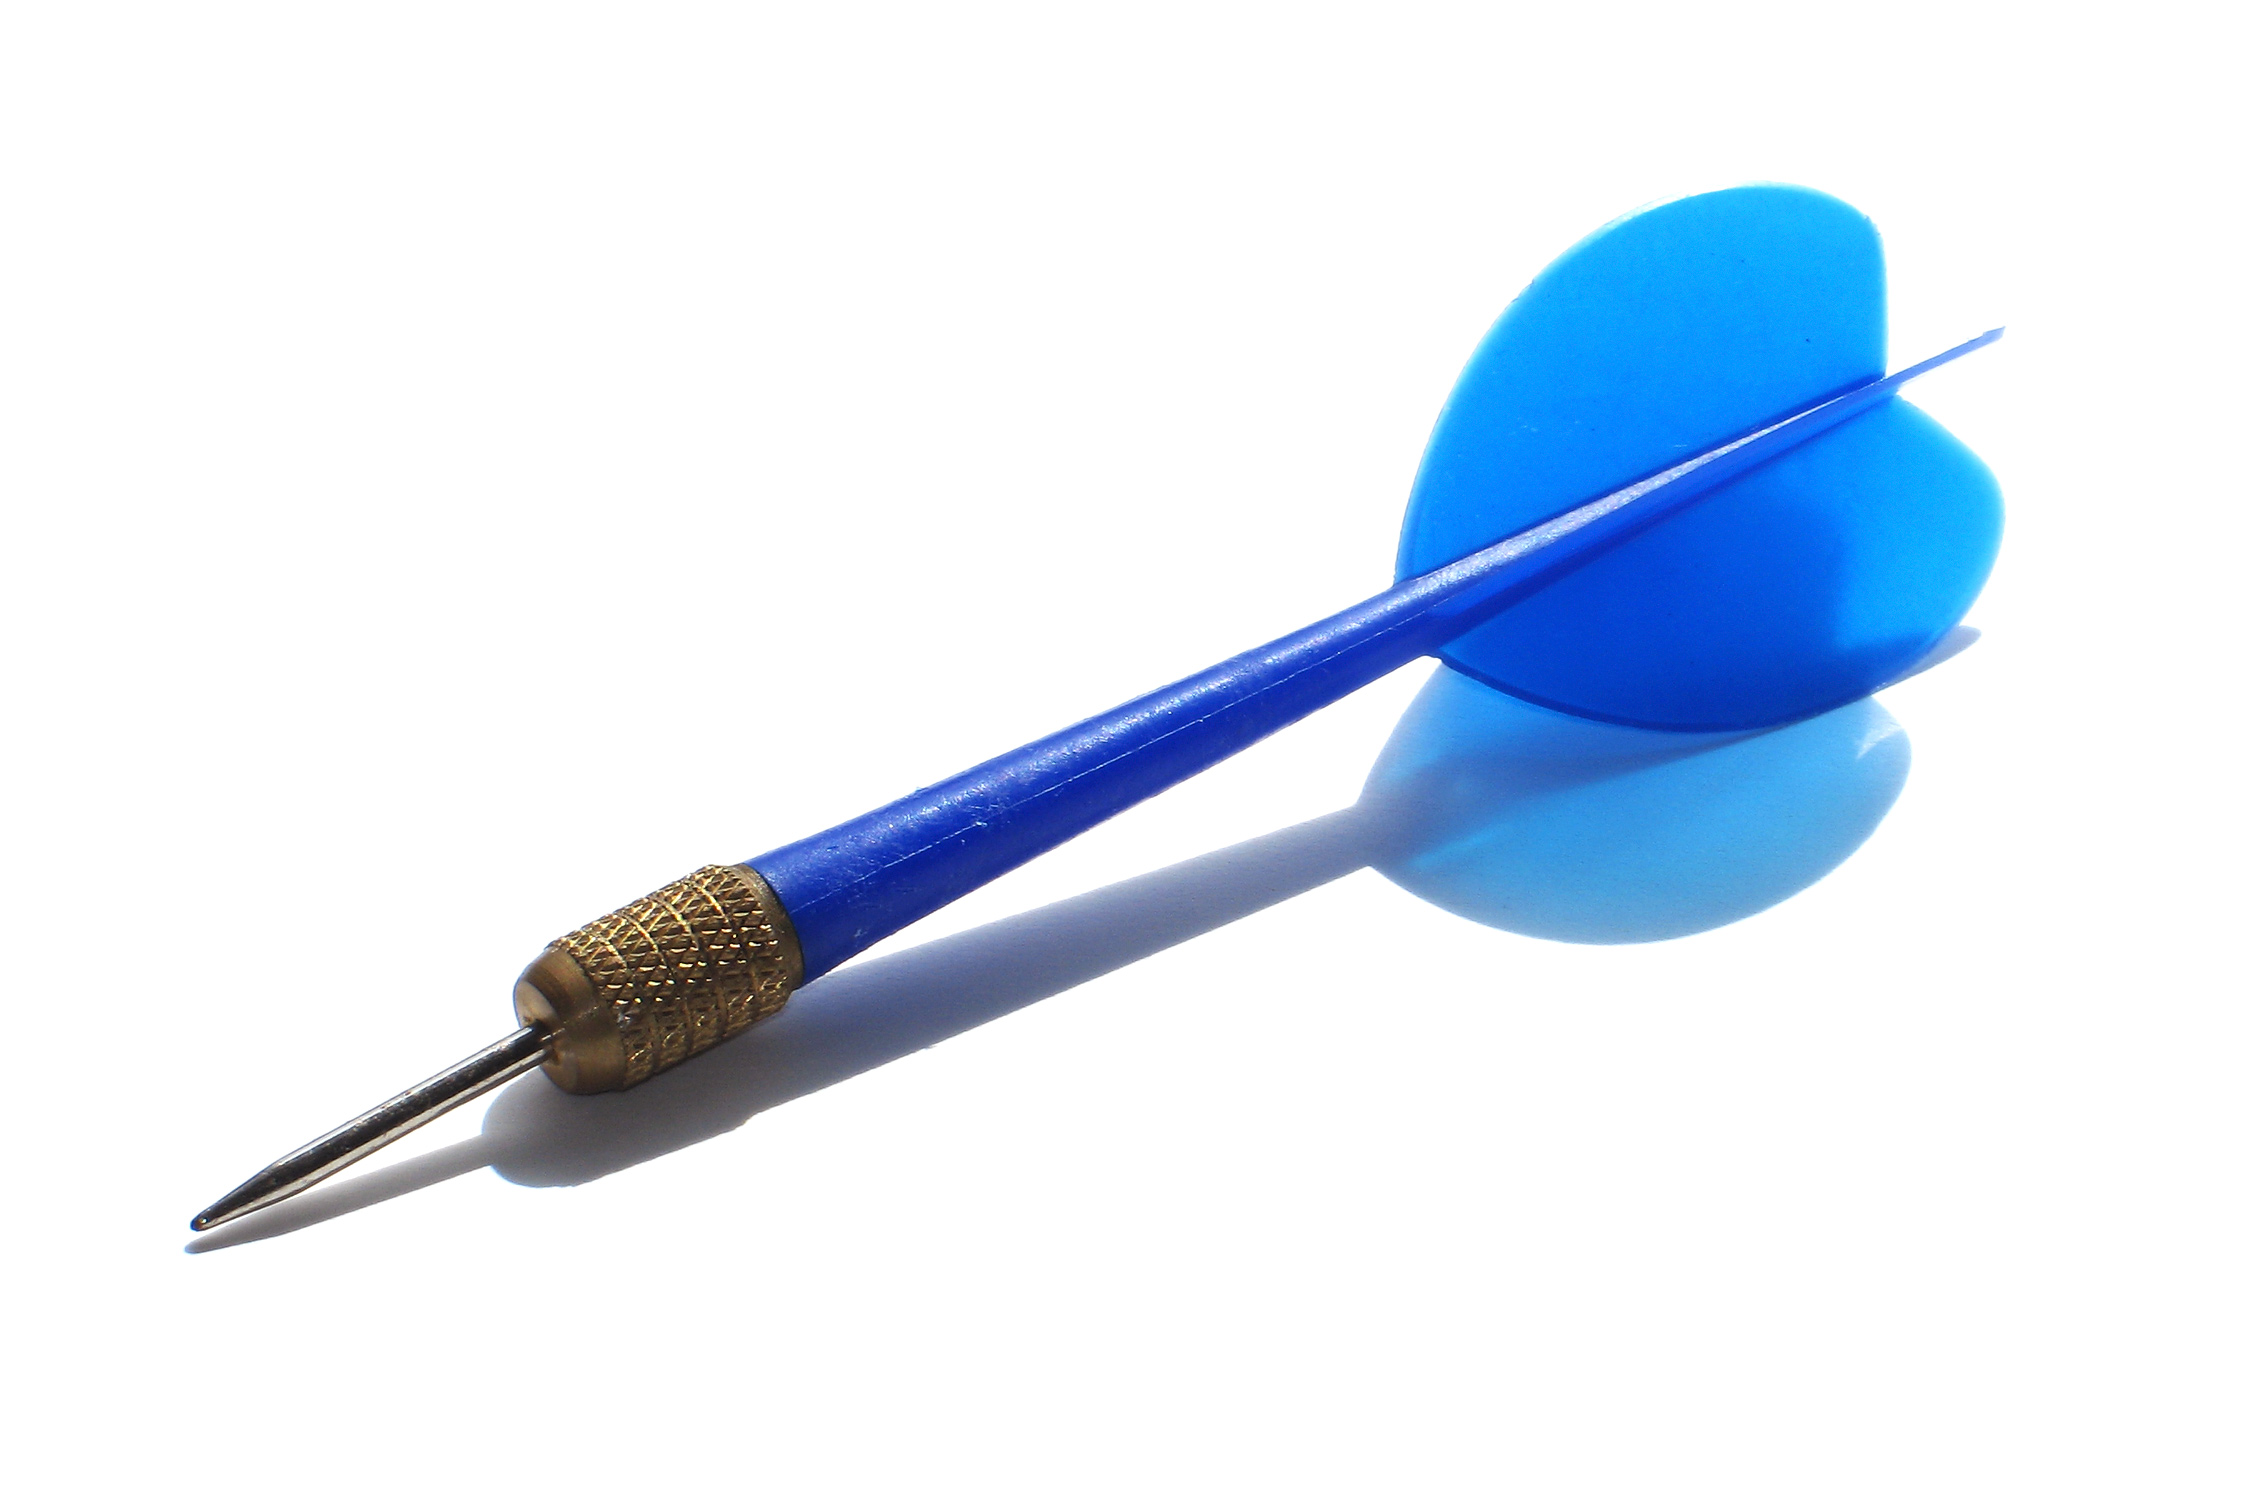
\includegraphics[width=5cm]{pictures/dart.jpg}
    \caption[Fléchette]{Exemple de fléchette respectant les normes officielles$^1$.}
    \label{fig:single_dart}
\end{figure}



La \textit{World Darts Federation} définit des critères à respecter pour l'installation et les parties de fléchettes. Ainsi, la cible doit respecter les dimensions suivantes :
\begin{itemize}
\item largeur intérieure des doubles et des triples : 8 mm
\item diamètre du centre (bulle) : 12,7 mm
\item diamètre du demi-centre (demi-bulle) : 31,8 mm
\item rayon du cercle extérieur de la couronne des doubles : 170 mm
\item rayon du cercle extérieur de la couronne des triples : 107,4 mm
\item diamètre total de la cible : 451 mm
\item épaisseur des fils : minimum 1,6 mm - maximum 1,8 mm
\end{itemize}

Le centre de la cible doit se trouver à 172,72 centimètres du sol, et la limite de tir est située à 2,37 mètres de la cible.

Les fléchettes doivent avoir une largeur inférieure à 3,38 centimètres et peuvent être de n'importe quelle longueur, tant que la distance allant de pointe au bout de l'empennage ne dépasse pas 20 centimètres. La masse d'une fléchette ne doit pas dépasser 50 grammes.

Les règles des différents jeux existants ne seront pas détaillées ici, car elles n'ont pas été utilisées dans le contexte de l'expérimentation. L'installation réalisée pour cette expérimentation respecte les dimensions et les distances imposées par la \textit{World Darts Federation}.

\footnotetext{source : https://fr.wikipedia.org/wiki/Fl\%C3\%A9chettes}

\subsubsection{Caractéristiques du mouvement et descripteurs considérés}
Des entretiens ont été réalisés avec un expert des fléchettes : Aurélien Orsini, président du \textit{Dart dart club de fléchettes mayennais} et champion régional en 2014. Ces entretiens ont pour but de prendre connaissance des modalités d'évaluation du geste de l'apprenant par l'expert lors d'une séance d'apprentissage, ainsi que des conseils prodigués pour améliorer le geste. Cette étape a permis de vérifier que les parties du corps et les modalités du mouvement regardées par l'expert sont formalisables en descripteurs opérationnalisables et en conséquence calculables à partir du mouvement enregistré. De ces entretiens sont ressortis quatre défauts majeurs souvent présents chez les débutants.

Le premier défaut est lié au fait de se pencher en avant (\textit{leaning}) durant le lancer. Lorsqu'un débutant lance une fléchette, son corps accompagne naturellement le geste en se penchant en avant (Fig. \ref{fig:darts_leaning_final})
. Ce défaut peut entraîner une visée plus basse que prévu, car le mouvement du corps imprime une rotation vers le bas au bras, par extension. Le conseil donné par l'expert est de rester fixe sur ses appuis, une fois en position de tir, tout en gardant le haut du corps (des hanches jusqu'à la tête) le plus immobile possible. Les descripteurs utilisés pour caractériser cet aspect du geste est la vitesse moyenne des épaules au cours du lancer : plus elle est basse, moins le haut du corps a bougé.

\begin{figure}
    \centering
    \includegraphics[width=10cm]{pictures/darts_leaning_final.png}
    \caption[Défaut du « leaning » (se pencher en avant)]{Défaut du « leaning » illustré : l'apprenant se penche en avant lors du lancer.}
    \label{fig:darts_leaning_final}
\end{figure}

Le deuxième défaut identifié est celui du mouvement du coude (\textit{elbow move}). Lors du lancer de fléchettes, le corps, ainsi que le bras, doivent rester le plus statique possible. Le mouvement de lancer doit s'effectuer à l'aide d'une rotation du coude, ce qui n'est possible que lorsque le bras est placé suffisamment en position de pré-lancer. Le problème usuel du geste d'un novice est que le bras et l'avant-bras forment un « V » avant le lancer, et finissent par former une ligne après le lancer, ce qui implique un déplacement du coude au cours du lancer. Le mouvement est ainsi moins maîtrisé que si le coude est la seule articulation qui pivote (Fig. \ref{fig:darts_elbow_move_final}). Le conseil donné par l'expert, dans ce cas, est de se concentrer sur l'immobilité du bras, afin que le coude effectue un pivot et que seul l'avant-bras ne bouge. Cet aspect du geste est caractérisé par les descripteurs de vitesse moyenne du coude, ainsi que de l'épaule (du côté de la préférence manuelle de l'utilisateur). Plus ces valeurs sont basses, moins le bras a bougé.

\begin{figure}
    \centering
    \includegraphics[width=10cm]{pictures/darts_elbow_move_final.png}
    \caption[Défaut du « elbow move » (déplacement du coude)]{Défaut du « elbow move » illustré : le coude de l'apprenant effectue un déplacement lors du lancer, au lieu de seulement effectuer une rotation.}
    \label{fig:darts_elbow_move_final}
\end{figure}

Un autre défaut possible est celui du " lancer de javelot " (\textit{javelin}). Lors d'un lancer, le bras, l'avant-bras et la main doivent rester devant le corps, dans l'alignement de l'axe tête-cible. Du début à la fin du mouvement, le bras, ainsi que la main, doivent toujours rester devant le corps. Or, chez les novices, le bras est souvent décalé (sur la gauche pour les gauchers, sur la droite pour les droitiers), et la prise d'élan du geste fait aller le bras à côté de la tête, voire même derrière (Fig. \ref{fig:darts_javelin_final}). Afin de détecter ce problème, la distance en x, y, et z de la main par rapport à la tête avant le lancer est utilisée.

\begin{figure}
    \centering
    \includegraphics[width=10cm]{pictures/darts_javelin_final.png}
    \caption[Défaut du « javelin » (lancer en javelot)]{Défaut du « javelin » illustré : la main de l'apprenant passe à côté (voire derrière) la tête lors de la prise d'élan du lancer.}
    \label{fig:darts_javelin_final}
\end{figure}

Le dernier défaut est celui de l'alignement du bras (\textit{align arm}). Un phénomène naturel lors du lancer est d'avoir un décalage entre l'alignement initial du bras et l'alignement final (lors du lancer). En effet, le bras a naturellement tendance à revenir vers le centre du corps, quelle que soit la préférence manuelle de la personne (droitier ou gaucher) (Fig. \ref{fig:darts_align_arm_final}). Il faut consciemment compenser cet effet, en essayant de garder un alignement équivalent du début à la fin du lancer. Afin de vérifier cet aspect du geste, une boîte englobante est calculée sur l'ensemble du geste. La moyenne de la largeur de cette boîte, ainsi que l'écart type, sont ensuite utilisés.

\begin{figure}
    \centering
    \includegraphics[width=10cm]{pictures/darts_align_arm_final.png}
    \caption[Défaut du « align arm » (alignement du bras)]{Défaut du « align arm » illustré : le bras de l'apprenant se dirige légèrement vers la droite lors du lancer (dans le cas d'un gaucher). L'effet inverse se produit pour un droitier.}
    \label{fig:darts_align_arm_final}
\end{figure}

Chaque défaut n'apparaît pas forcément indépendamment des autres : dans la réalité, les apprenants cumulent très souvent plusieurs de ces défauts. Il existe également d'autres défauts, tels que la mauvaise prise d'une fléchette, un mauvais relâchement de la fléchette (qui lui imprime un mouvement erratique), etc. Ces problèmes ne sont cependant pas détectables à l'aide du mouvement de l'apprenant seul. Ils nécessitent d'autres données (telles que la position de la fléchette, la connaissance du moment du lâcher de fléchette, etc.) qu'il n'est pas possible d'obtenir à l'aide du matériel utilisé pour cette expérimentation.

\subsection{Protocole}
\subsubsection{Acquisition des données de l'expert}
La première étape est la captation des données de l'expert, afin d'intégrer les besoins d'observation de l'expert au sein du système. L'objectif est d'obtenir des données correspondant à des mouvements jugés corrects par l'expert, et des données avec les défauts pris séparément. Ainsi, l'expert a réalisé dix lancers de fléchettes bons, puis dix lancers pour chacun des quatre défauts identifiés. Puis, pour chaque défaut, les descripteurs correspondants sur les bons mouvements, et sur les mouvements présentant le défaut considéré sont extraits.

\subsubsection{Participants}
Trois groupes de 15 personnes chacun ont participé à l'expérimentation. Dans ces trois groupes, aucune personne n'était experte des fléchettes : le plus souvent, les seules connaissances de ce sport provenaient d'une pratique peu fréquente en tant que loisir. Le premier groupe n'a reçu que des conseils de l'expert, le deuxième n'a reçu que des conseils provenant du système MLA, et le troisième recevait des conseils de l'expert qui s'appuyait sur une visualisation des défauts donnée par le système pour donner son jugement. L'installation finale de l'expérimentation est présentée sur la Fig. \ref{fig:Darts_scheme}.

\begin{figure}
    \centering
    \includegraphics[width=\textwidth]{pictures/Darts_scheme.png}
    \caption{Installation de l'expérimentation.}
    \label{fig:Darts_scheme}
\end{figure}

\subsubsection{Déroulement}
Avant l'expérimentation, un pré-questionnaire était rempli par chaque participant, afin de recueillir sa taille (pour fournir un squelette adapté dans le logiciel de capture de mouvements), le niveau d'expertise autoévalué aux fléchettes (échelle de Likert à 7 réponses), ainsi que toute pratique actuelle d'un sport (voir Annexe 1).

Une fois ce pré-questionnaire rempli, la combinaison de capteurs était installée sur la personne. Les calibrations étaient ensuite effectuées, afin d'étalonner les capteurs (position dans l'espace, espacement des capteurs entre eux, mise à zéro sur le logiciel de capture, etc.) pour que le logiciel puisse adapter la combinaison par rapport aux articulations du squelette 3D.

Chaque participant a reçu comme instruction de viser le centre de la cible à l'aide de fléchettes. La position de lancer étant importante, il a été demandé de se placer perpendiculairement à la marque au sol (Fig. \ref{fig:darts_position}).

\begin{figure}
    \centering
    \includegraphics[width=7cm]{pictures/darts_position.jpg}
    \caption{Position latérale imposée aux participants.}
    \label{fig:darts_position}
\end{figure}

Les participants devaient ensuite effectuer neuf lancers de test, non enregistrés. Ces lancers avaient pour buts de permettre à la personne de s'habituer à la combinaison et au lancer, ainsi que de vérifier que le squelette ne présentait pas de problèmes lors du mouvement (dérive des capteurs, mauvais positionnement des capteurs, parties de la combinaison qui ne fonctionnent pas, etc.).

Chaque personne a été affectée à l'un des trois groupes expérimentaux, sans avoir connaissance de cette assignation. Afin d'éviter toute différence de perception, il a été dit à chaque personne que les conseils étaient donnés par le système (même si ce n'était pas le cas pour tous les groupes).

Avant chaque lancer, la personne doit se placer en position de lancer, dire « prêt », puis attendre le signal sonore de départ du logiciel (qui correspond au début de l'enregistrement du mouvement). La personne lance ensuite sa fléchette, puis garde la position finale de son bras jusqu'au deuxième signal sonore (correspondant à l'arrêt de l'enregistrement). L'intervalle de temps entre le premier signal sonore et le lancer varie grandement d'une personne à l'autre ; cependant, l'algorithme de segmentation permet de ne garder que le geste utile pour chaque participant (cf. chapitre \ref{chap:traitement_donnees} section \ref{subsec:MoI}). À chaque lancer, la distance de la fléchette par rapport au centre est relevée (Fig. \ref{fig:target_with_darts_distance}).

\begin{figure}
    \centering
    \includegraphics[width=7cm]{pictures/target_with_darts_distance.jpg}
    \caption[Distance relevée entre les fléchettes et le centre de la cible]{En bleu, la distance relevée après chaque lancer de fléchette.}
    \label{fig:target_with_darts_distance}
\end{figure}

Chaque personne a effectué quatre séries de neuf lancers, soit trente-six lancers au total. Au bout d'une série de neuf lancers, les mouvements étaient analysés par le système (indépendamment du fait que les conseils donnés proviennent du système ou non). Pour le premier groupe, les données étaient analysées mais non utilisées par l'expert pour le jugement du geste. Chaque personne recevait alors deux conseils par rapport à son geste. En fonction de son groupe (conseils de l'expert pour le groupe 1, conseils du système pour le groupe 2, conseils de l'expert assisté du système pour le groupe 3). Les conseils donnés (par le système ou l'expert) sont les suivants :
\begin{itemize}
	\item corps penché : « Votre corps et vos épaules ne doivent pas bouger pendant votre lancer. »
	\item lancer type javelot : « Votre main doit toujours rester devant votre corps lorsque vous lancez. »
	\item alignement du bras : « Votre bras doit rester aligné (de la main à l'épaule) lorsque vous lancez. »
	\item mouvement du coude : « Votre coude ne doit pas bouger lors du lancer. »
\end{itemize}

Dans le cas du groupe deux, les conseils sont choisis comme il suit :
\begin{itemize}
	\item La distance entre le centroïde des données de l'apprenant et du cluster de gestes cibles de l'expert est calculée, pour chaque défaut (voir chapitre \ref{chap:traitement_donnees} section \ref{subsec:feedback})
	\item Si deux défauts sont situés soit (i) dans le trapèze reliant les deux clusters, soit (ii) dans le cluster de mauvais gestes de l'expert, les deux conseils correspondant à ces défauts sont donnés
	\item S'il n'y en a qu'un seul, le conseil correspondant au défaut situé dans la zone susmentionnée est donné, puis le conseil correspondant au défaut dont la distance est la plus éloignée du bon cluster est donné
	\item S'il n'y en a aucun, les deux conseils correspondant aux défauts dont les distances sont les plus éloignées du bon cluster sont donnés
\end{itemize}

Dans le cas du groupe 3, une visualisation des données de l'apprenant par rapport à celles de l'expert est proposée (Fig. \ref{fig:feedback_grp_example}). Ainsi, l'expert peut s'appuyer sur cette visualisation pour prendre sa décision. Cette visualisation permet également de compenser un cas particulier : si les données de l'apprenant sont très dispersées, mais centrées autour du cluster de bons mouvements de l'expert, le centroïde des données de l'apprenant sera situé dans le cluster de bons gestes de l'expert. Ainsi, il est possible pour l'expert de repérer ce cas particulier dans le cas où il s'appuie sur le système pour donner ses conseils, et de ne pas considérer que cet aspect des gestes de l'apprenant est réussi. Cependant, dans le cadre de l'expérimentation, l'expert s'est basé sur les valeurs de distance affichées directement, plutôt que sur la visualisation. Il procède comme il suit :
\begin{itemize}
	\item s'il décèle deux défauts, les deux conseils correspondant à ces défauts sont donnés à l'apprenant,
	\item s'il décèle un seul défaut, il donne le conseil correspondant à ce défaut, puis se base sur les valeurs de distance affichées par le système afin de donner le conseil sur le défaut étant le plus éloigné du cluster de bons gestes,
	\item s'il n'arrive pas à déceler de défauts, il se base sur les valeurs de distance affichées par le système, et choisit les deux défauts les plus éloignés du bon cluster.
\end{itemize}


\begin{figure}
    \centering
    \includegraphics[width=15cm]{pictures/feedback_grp_example.png}
    \caption[Exemple de visualisation à la fin des séries de lancer]{Un exemple de visualisation des données de l'apprenant fournie à l'expert à la fin d'une série de neuf lancers.}
    \label{fig:feedback_grp_example}
\end{figure}

La personne refaisait ensuite 9 lancers, en essayant de tenir compte de ces deux conseils. Il n'y a pas de conseils donnés à la fin de la dernière série.

Une fois l'expérimentation finie, la personne remplit un post-questionnaire (voir Annexe 1). Ce post-questionnaire mesure le ressenti de la personne par rapport à la combinaison, à la progression de son geste et à l'auto-évaluation de sa performance. Les questions sont toutes basées sur l'échelle de Lickert, allant de 1 à 7. Les questions portent sur :
\begin{itemize}
	\item le niveau d'aisance avec le matériel,
	\item le niveau de stress de l'apprenant lors de l'expérimentation,
	\item le niveau de compréhension des instructions reçues,
	\item l'intérêt ressenti des conseils donnés,
	\item l'auto-évaluation de la performance sur toute l'expérimentation,
	\item l'auto-évaluation de la progression de la performance sur toute l'expérimentation,
	\item l'auto-évaluation de la qualité du geste sur toute l'expérimentation,
	\item l'auto-évaluation de la progression de la qualité du geste sur toute l'expérimentation,
	\item l'expression libre (remarques diverses).
\end{itemize}


\subsubsection{Métriques calculées sur le clustering des données de l'expert}
L'algorithme utilisé afin de regrouper les données de l'expert est un \textit{k-means}, avec $k = 2$. Les métriques d'ASS et d'ARI ont été calculées sur les regroupements obtenus (voir tableau \ref{tab:ass_ari_darts}).

\begin{table}[h]
\centering
\begin{tabular}{c|c|c}
& Silhouette Score & Adjusted Rand Index\\\hline
Leaning & 0.85 & 1\\
elbow move & 0.58 & 0.47\\
javelin & 0.79 & 1\\
align arm & 0.53 & 1\\
\end{tabular}
\caption{Valeurs de l'Average Silhouette Score et de l'Adjusted Rand Index pour les données de l'expert sur les quatre défauts.}
\label{tab:ass_ari_darts}
\end{table}

Les valeurs pour l'\textit{ASS} sont supérieures ou égales à celles obtenues pour les deux expérimentations précédentes, suggérant une bonne (voire très bonne) séparation des données. L'hypothèse \textbf{H3} est validée dans le contexte de cette expérimentation. Les valeurs pour l'\textit{ARI} suggèrent que le regroupement des données d'un défaut (mouvement du coude) ne correspond pas exactement à la vérité terrain relevée. Cela implique que certaines des données de l'expert ne sont pas séparables de manière fidèle à la vérité terrain à l'aide des descripteurs utilisés. Cela peut s'expliquer soit par (i) un mauvais choix de descripteurs, soit par (ii) des mouvements de l'expert où la différence entre le geste correct et le défaut n'est pas assez prononcée. Dans ces cas, le clustering permet d'obtenir un regroupement des données selon leur similitude, plutôt que l'étiquetage relevé.

\subsection{Résultats}
Les résultats de l'expérimentation ont été analysés sous deux angles : l'amélioration de l'objectif du mouvement (c'est-à-dire la distance des fléchettes par rapport au centre de la cible) et l'amélioration des propriétés du mouvement de l'apprenant (c'est-à-dire le rapprochement du centroïde de l'apprenant du cluster de l'expert pour chaque défaut). L'analyse a été réalisée sous deux aspects : l'analyse intergroupes pour chaque jeu de lancers, et l'analyse intragroupe, sur les quatre jeux pour chaque groupe. L'objectif est double : (i) vérifier qu'il y a une amélioration significative du geste (au sens des tests statistiques effectués) au cours de l'expérimentation, que le système soit utilisé ou non et (ii) vérifier l'existence d'une différence significative (au sens des tests statistiques effectués) de l'amélioration du geste en fonction de l'utilisation faite du système : expert assisté, système seul ou sans système.

\subsubsection{Tests utilisés}

Deux tests de normalité sont utilisés pour évaluer si la distribution des données suit une loi normale : le test de Shapiro-Wilk, et le test d'Agostino-Pearson. Plus précisément, le test de Shapiro-Wilk teste l'hypothèse nulle selon laquelle la population est normalement distribuée. Bien que ce test soit parfois recommandé pour tester la normalité de données \parencite{Thode2002Tfn} et soit très largement utilisé, il n'est que peu efficace lorsque plusieurs données ont la même valeur. Ainsi, le test d'Agostino-Pearson est également utilisé, permettant de pallier ce problème \parencite{DAgostino1990ASf}.
Le niveau alpha de comparaison utilisé est $0.05$ dans les deux cas.

La distribution de la population selon une loi normale permet d'utiliser des tests paramétriques, plus précis que leurs contreparties non-paramétriques (qui ne font aucune hypothèse sur la distribution des données). Dans le cas des données analysées, la distribution ne suit pas systématiquement une loi normale. Les résultats des tests paramétriques et non-paramétriques sont présentés dans les tableaux, mais seuls les tests pertinents au regard de la distribution des données sont analysés.

Pour l'analyse intergroupe, 15 personnes différentes pour chaque groupe ont réalisé l'expérimentation. Nous supposerons donc que les échantillons de données résultants de l'activité humaine, dans le contexte de cette expérimentation, sont indépendants entre les groupes.

\paragraph{Tests pour les résultats intergroupe}
Dans le cas d'une distribution normale de la population, où l'on compare deux échantillons issus de populations différentes, les tests utilisés sont des tests paramétriques. Le test choisi ici est l'ANOVA (\textit{\textbf{AN}alysis \textbf{O}f \textbf{VA}riance}). Son objectif est de déterminer si les distributions suivent une même loi normale (hypothèse nulle) ou si au moins une des moyennes des distributions est différente de celles des autres échantillons (hypothèse alternative). Si l'hypothèse nulle est vérifiée, l'homogénéité des variances des groupes est alors vérifiée à l'aide du test de Levene. Dans ce test, l'hypothèse nulle stipule que les variances de population sont égales. Enfin, un test de Student paire-à-paire est effectué, afin d'identifier les différences significatives entre les groupes pris deux-à-deux.\\

Dans le cas où la distribution de la population ne suit pas une loi normale, les tests non-paramétriques sont utilisés. Ces tests nécessitent plus de données que leur contrepartie paramétrique. Le premier test utilisé est celui de Kruskal-Wallis ; il est la contrepartie non-paramétrique du test d'ANOVA. L'hypothèse nulle est que les médianes de chaque groupe sont égales, l'hypothèse alternative étant qu'au moins une médiane d'un groupe est différente d'au moins l'une de celles des autres groupes. Si l'hypothèse nulle est vérifiée, un test de Wilcoxon-Mann-Whitney est utilisé, afin de tester si les distributions sont égales (hypothèse nulle).


Pour l'analyse intragroupe, dans chacun des groupes pris indépendamment, les 15 mêmes personnes réalisent chacun des 4 jeux de lancers à la suite. Nous supposerons donc que les échantillons de données résultants de l'activité humaine, dans le contexte de cette expérimentation, sont dépendants entre les jeux.

\paragraph{Tests pour les résultats intragroupes}
Dans le cas où la distribution de la population suit une loi normale, le test de Student sur deux échantillons est utilisé. L'hypothèse nulle de ce test stipule que la moyenne des deux populations est égale.\\

Dans le cas où la distribution de la population ne suit pas une loi normale, le test non-paramétrique utilisé est le test des rangs signés de Wilcoxon (la contrepartie non-paramétrique du test de Student sur deux échantillons). L'hypothèse nulle de ce test est que la médiane de deux échantillons est égale.
\vspace{0.5cm}


Dans tous les cas considérés, il faut noter que le rejet ou la validation de l'hypothèse nulle n'est pas une preuve formelle que les résultats sont reproductibles et valides \parencite{Halsey2015Tfp}. Lorsque l'hypothèse nulle est rejetée, le résultat est considéré comme significatif et n'est pas dû à un phénomène aléatoire. Cependant, ce n'est pas une preuve formelle que la différence significative obtenue entre les échantillons soit liée à leur condition expérimentale respective identifiée par le chercheur. L'interprétation des résultats significatifs obtenus en comparant les différences dans les conditions expérimentales doit être menée avec une grande prudence et se limiter au cadre expérimental défini. La reproductibilité des résultats ne peut être alors qu'envisagée dans les limites du cadre, tandis que la généralisation peut être uniquement supposée. À l'inverse, lorsque l'hypothèse nulle est validée, il n'est généralement pas utile de pousser plus loin l'interprétation des résultats obtenus.

Cette partie ne présentera que les résultats pertinents au regard des tests considérés. Les tableaux complets d'analyse sont disponibles dans l'annexe 2.

Pour chaque analyse, les données sont affichées sous forme de diagrammes en boîte. Ces diagrammes, également appelés boîtes à moustaches, permettent de visualiser :
\begin{itemize}[label=$-$]
	\item la moyenne (losange noir),
	\item la médiane (barre noire),
	\item les valeurs du premier et troisième quartile (l'extrémité basse et haute des boîtes, respectivement),
	\item la différence entre $q_3$ et $q_1$ est appelée écart interquartile, et est défini par la différence $q_3 - q_1$,
	\item les limites (moustaches) représentées respectivement par les points les plus proches de $q_1 - \frac{q_3 - q_1}{1.5}$ et $q_3 + \frac{q_3 - q_1}{1.5}$,
	\item la dispersion, représentée par l'écart entre les limites (moustaches),
	\item les données aberrantes, situées en deçà ou au-delà des limites (points rouges).
\end{itemize}


\subsubsection{Distance des fléchettes par rapport au centre de la cible}

Le tableau \ref{tab:moy_std_precision} présente les moyennes et les écarts-types des distances des fléchettes par rapport au centre de la cible lors des lancers des participants. On remarque une dégradation systématique de la moyenne, ainsi que de l'écart-type, entre le jeu 1 et le jeu 2. Ces valeurs tendent à diminuer pour les jeux suivants, sauf dans le cas du groupe 3, ou la valeur augmente entre le jeu 2 et le jeu 3, puis diminue ensuite. La différence entre le jeu 1 et le jeu 4 montre que ces valeurs se rapprochent des valeurs initiales. Ces résultats suggèrent que les premiers conseils donnés entraînent une perte de précision du geste, puis que les participants réussissent à améliorer la précision de leurs lancers.

\begin{table}[]
\small
\makebox[\textwidth][c]{
\begin{tabular}{l|llllllll}
 & \multicolumn{2}{c}{Jeu 1} & \multicolumn{2}{c}{Jeu 2} & \multicolumn{2}{c}{Jeu 3} & \multicolumn{2}{c}{Jeu 4} \\
 & Moyenne & Écart-Type & Moyenne & Écart-Type & Moyenne & Écart-Type & Moyenne & Écart-Type \\\hline
Groupe 1 & 10.1481 & 3.8336 & 14.4170 & 5.4708 & 10.9926 & 3.2721 & 10.2481 & 3.5990 \\
Groupe 2 & 10.2481 & 3.6957 & 13.5741 & 6.4499 & 11.9674 & 4.6060 & 10.9296 & 3.6617 \\
Groupe 3 & 9.7393 & 2.3020 & 11.9667 & 4.0647 & 12.6889 & 5.7258 & 11.0074 & 5.4516
\end{tabular}}
\caption{Moyennes et écarts-types des données des apprenants (distance au centre de la cible).}
\label{tab:moy_std_precision}
\end{table}

Les résultats intergroupes sont présentés dans la figure \ref{fig:Precision_All_data_intergroupe}. Pour chaque jeu (un jeu par graphique), les données des trois groupes sont présentées en parallèle. La figure \ref{fig:Precision_All_data_intragroupe} montre la progression de la précision en intra-groupe pour chaque groupe (un groupe par graphique).

Sur la figure \ref{fig:Precision_All_data_intragroupe}, on peut observer une augmentation systématique de la valeur de la médiane ainsi que de la dispersion des données entre le jeu 1 et le jeu 2 pour tous les groupes, correspondant à une augmentation de la distance par rapport au centre. S'en suit une réduction de la dispersion des valeurs pour les jeux suivants (sauf pour le jeu 4 du groupe 3), suggérant ainsi une précision des lancers en hausse. Cependant, la précision ne revient pas à une valeur inférieure ou égale à celle du premier jeu (en terme de médiane, moyenne et précision). Cette tendance est la plus visible pour le groupe 1. Des résultats significatifs ont été obtenus entre les jeux 1 et 2 et les jeux 2 et 4 pour chaque groupe (tableau \ref{tab:precision_intra}), montrant d'une part une dégradation systématique de la distance par rapport au centre de la cible à la suite des premiers conseils donnés, quel que soit le groupe considéré, et une amélioration progressive de la précision du lancer au fil de l'expérimentation. Des résultats significatifs ont également été obtenus entre le jeu 1 et le jeu 3 pour les groupes 2 et 3, le jeu 2 et le jeu 3 pour le groupe 1 et le jeu 3 et le jeu 4 pour le groupe 3. Cette dégradation semble correspondre au « désapprentissage » du geste initial au profit de l'apprentissage du geste cible. On constate la présence de données aberrantes sur les trois groupes, dont au moins une persistante sur les quatre jeux pour les groupes 2 et 3. Il y a plus de données aberrantes pour le groupe 3 (entre une et trois, selon le jeu considéré), malgré le fait que ce groupe soit celui présentant les meilleures valeurs de médianes, écart interquartile et dispersion.


Pour l'analyse intergroupe (figure \ref{fig:Precision_All_data_intergroupe}), on observe que le groupe 3 est celui dont l'écart interquartile est le plus faible sur tous les jeux sauf le quatrième (groupe 1), tout en ayant le plus de données aberrantes. Le groupe 1 est celui ayant la médiane la plus basse sur tous les jeux, sauf le deuxième (groupe 3). Dans les deux cas, les résultats ne présentent pas de différences significatives (tableau \ref{tab:precision_inter}).
\afterpage{
\begin{landscape}
\begin{table}[]
\centering
\begin{tabular}{ll|ccccc|cccc}
    &  & \multicolumn{5}{c|}{Wilcoxon Signed-Rank ($p < 0.05$)} & \multicolumn{4}{c}{T Test ($p < 0.05$)} \\ \cline{3-11}
    &  & \multicolumn{2}{c|}{One tail} & \multicolumn{2}{c}{Two tails} &  & \multirow{2}{*}{One tail} & \multirow{2}{*}{Two tails} & \multirow{2}{*}{t} & \multirow{2}{*}{df} \\ \cline{3-7}
    &  & p-norm & p-exact & p-norm & p-exact & T &  &  &  &  \\ \hline
 \multirow{3}{*}{Jeu 1-2} & G1 & \cellcolor{green!25} 0.0057 & \cellcolor{green!25} 0.0042 & \cellcolor{green!25} 0.0115 & \cellcolor{green!25} 0.0084 & 15 &  &  &  &  \\
 & G2 & \cellcolor{green!25} 0.0021 & \cellcolor{green!25} 0.0010 & \cellcolor{green!25} 0.0041 & \cellcolor{green!25} 0.0020 & 9 &  &  &  &  \\
 & G3 & \cellcolor{green!25} 0.0038 & \cellcolor{green!25} 0.0021 & \cellcolor{green!25} 0.0076 & \cellcolor{green!25} 0.0043 & 12.5 &  &  &  &  \\ \hline
\multirow{3}{*}{Jeu 2-3} & G1 & \cellcolor{green!25} 0.0049 & \cellcolor{green!25} 0.0034 & \cellcolor{green!25} 0.0098 & \cellcolor{green!25} 0.0067 & 14 &  &  &  &  \\
 & G2 & 0.1006 & 0.1039 & 0.2013 & 0.2078 & 37 &  &  &  &  \\
 & G3 & 0.5 & 0.4890 & 1 & 0.9780 & 59.5 &  &  &  &  \\ \hline
\multirow{3}{*}{Jeu 3-4} & G1 &  &  &  &  &  & 0.1514 & 0.3028 & 1.0698 & 14 \\
 & G2 & 0.1221 & 0.1262 & 0.2443 & 0.2524 & 39 & 0.1439 & 0.2877 & 1.1052 & 14 \\
 & G3 & \cellcolor{green!25} 0.0144 & \cellcolor{green!25} 0.0128 & \cellcolor{green!25} 0.0288 & \cellcolor{green!25} 0.0256 & 21 &  &  &  &  \\ \hline
\multirow{3}{*}{Jeu 1-3} & G1 & 0.1601 & 0.1651 & 0.3202 & 0.3303 & 42 &  &  &  &  \\
 & G2 & 0.1110 & 0.1146 & 0.2220 & 0.2293 & 38 &  &  &  &  \\
 & G3 & \cellcolor{green!25} 0.01659 & \cellcolor{green!25} 0.0151 & \cellcolor{green!25} 0.0332 & \cellcolor{green!25} 0.0301 & 22 &  &  &  &  \\ \hline
\multirow{3}{*}{Jeu 2-4} & G1 & \cellcolor{green!25} 0.0005 & \cellcolor{green!25} $9.1553e^{-5}$ & \cellcolor{green!25} 0.0011 & \cellcolor{green!25} 0.0002 & 2 &  &  &  &  \\
 & G2 & \cellcolor{green!25} 0.0073 & \cellcolor{green!25} 0.0051 & \cellcolor{green!25} 0.0146 & \cellcolor{green!25} 0.0102 & 16.5 &  &  &  &  \\
 & G3 & \cellcolor{green!25} 0.0250 & \cellcolor{green!25} 0.0240 & \cellcolor{green!25} 0.0500 & \cellcolor{green!25} 0.0479 & 25 &  &  &  &  \\ \hline
\multirow{3}{*}{Jeu 1-4} & G1 & 0.4660 & 0.4670 & 0.9321 & 0.9341 & 58 &  &  &  &  \\
 & G2 & 0.0864 & 0.0844 & 0.1728 & 0.1688 & 35.5 &  &  &  &  \\
 & G3 & 0.2051 & 0.2106 & 0.4102 & 0.4212 & 45 &  &  &  &
\end{tabular}
\caption{Résultats des tests statistiques en intragroupe (distance par rapport au centre).}
\label{tab:precision_intra}
\end{table}
\end{landscape}}

\begin{table}[]
\centering
\begin{tabular}{lr|cccc}
 &  & Jeu 1 & Jeu 2 & Jeu 3 & Jeu 4 \\\hline
\multirow{2}{*}{ANOVA} &  &  &  &  &  \\
 &  &  &  &  &  \\\hline
\multirow{3}{*}{Pairwise T-test} & & & & & \\
 & & & & &  \\
 & & & & &  \\\hline
\multirow{3}{*}{Kruskal-Wallis ($p < 0.05$)} & Chi-square & 0.1875 & 1.8023 & 0.4432 & 0.3937 \\
 & p & 0.9907 & 0.4061 & 0.8012 & 0.8213 \\
 & df & 2 & 2 & 2 & 2 \\\hline
\multirow{3}{*}{Pairwise Mann-Whitney} & & & & & \\
 & & & & & \\
 & & & & &
\end{tabular}
\caption{Résultats des tests statistiques en intergroupe (distance par rapport au centre).}
\label{tab:precision_inter}
\end{table}


\begin{figure}%[H]
	\centering
	\makebox[\textwidth][c]{
    \includegraphics[width=15cm]{expe_results/Precision_All_data_intragroupe.png}}
    \caption[Moyennes des distances des fléchettes par rapport au centre en intra-groupe]{Moyennes des distances des fléchettes par rapport au centre de la cible en intra-groupe.}
    \label{fig:Precision_All_data_intragroupe}
\end{figure}


\begin{figure}%[H]
	\centering
	\makebox[\textwidth][c]{
    \includegraphics[width=15cm]{expe_results/Precision_All_data_intergroupe.png}}
    \caption[Moyennes des distances des fléchettes par rapport au centre en inter-groupe]{Moyennes des distances des fléchettes par rapport au centre de la cible en inter-groupe.}
    \label{fig:Precision_All_data_intergroupe}
\end{figure}



\subsubsection{Amélioration des défauts du mouvement}

Le tableau \ref{tab:advices_freq} montre la fréquence à laquelle sont donnés les conseils entre chaque jeu. On remarque qu'après le premier jeu, le défaut du corps penché est plus détecté que les autres, à l'inverse du défaut de l'alignement du bras. Cela peut s'expliquer par la facilité d'observation du défaut du corps penché par l'expert, à l'inverse de l'alignement du bras à cause de la position d'observation (visible sur la figure \Ref{fig:Darts_scheme}). À l'inverse, pour les conseils donnés à la fin du jeu 3, le défaut du corps penché est moins donné, car souvent corrigé dès les premiers jeux.

Le tableau \ref{tab:advices_groupes_freq} présente la fréquence des conseils donnés pour chaque groupe, entre chaque jeu et pour chaque groupe. Ainsi, on peut constater que le défaut du corps penché est très souvent détecté comme étant le défaut à corriger en premier, quel que soit le groupe considéré. Ce défaut est en fait une caractéristique des lancers de manière générale : se pencher lors d'un lancer permet d'imprimer plus de force au projectile. Pour le groupe 1, le conseil le plus donné est celui du mouvement du coude. Ce défaut est facilement observable lors du geste d'un apprenant, et donc l'expert tend à se concentrer sur ce défaut tant qu'il n'estime pas le mouvement satisfaisant. À l'inverse, le défaut du lancer de type javelot est rarement considéré par l'expert. En effet, il est plus difficilement observable que les autres dans le contexte de cette expérimentation. Le système seul tend à donner les conseils sur les mêmes deux défauts pour les deux premiers jeux, à savoir le lancer de type javelot et le corps penché. Pour le troisième jeu, la fréquence des conseils s'harmonise, suggérant ainsi une stabilisation au niveau de tous les défauts (sans pour autant systématiquement atteindre une correction acceptable). Enfin, on remarque que le groupe 3 est celui présentant la répartition de conseils la plus homogène.

%\begin{table}[]
%\begin{tabular}{l|lll}
%           & jeu 1-2 & jeu 2-3 & jeu 3-4 \\\hline
%align arm  & 8       & 21      & 24      \\
%elbow move & 24      & 26      & 27      \\
%javelin    & 24      & 22      & 22      \\
%leaning    & 34      & 21      & 17
%\end{tabular}
%\caption{Fréquence des conseils donnés (en pourcentage) en fonction des jeux.}
%\label{tab:advices_freq_base}
%\end{table}
%
%\begin{table}[]
%\begin{tabular}{llll}
%           & jeu 1-2 & jeu 2-3 & jeu 3-4 \\
%align arm  & 9       & 23      & 27      \\
%elbow move & 27      & 29      & 30      \\
%javelin    & 26      & 25      & 24      \\
%leaning    & 38      & 23      & 19
%\end{tabular}
%\caption{Fréquence des conseils donnés (en pourcentage) en fonction des jeux.}
%\label{tab:advices_freq_perc}
%\end{table}

\begin{table}%[H]
\centering
\begin{tabular}{l|lll}
           & jeu 1-2 & jeu 2-3 & jeu 3-4 \\\hline
align arm  & 0.09      & 0.23      & 0.27      \\
elbow move & 0.27      & 0.29      & 0.30      \\
javelin    & 0.26      & 0.25      & 0.24      \\
leaning    & 0.38      & 0.23      & 0.19
\end{tabular}
\caption{Fréquences des conseils donnés en fonction des jeux.}
\label{tab:advices_freq}
\end{table}

%\begin{table}[]
%\begin{tabular}{ll|llll}
%                    &         & align arm & elbow move & javelin & leaning \\\hline
%\multirow{3}{*}{G1} & Jeu 1-2 & 3         & 13         & 3       & 11      \\
%                    & Jeu 2-3 & 10        & 10         & 6       & 4       \\
%                    & Jeu 3-4 & 11        & 12         & 2       & 5       \\\hline
%\multirow{3}{*}{G2} & Jeu 1-2 & 2         & 3          & 14      & 11      \\
%                    & Jeu 2-3 & 4         & 5          & 10      & 11      \\
%                    & Jeu 3-4 & 6         & 6          & 11      & 7       \\\hline
%\multirow{3}{*}{G3} & Jeu 1-2 & 3         & 8          & 7       & 12      \\
%                    & Jeu 2-3 & 7         & 11         & 6       & 6       \\
%                    & Jeu 3-4 & 7         & 9          & 9       & 5
%\end{tabular}
%\caption{Fréquence des conseils donnés pour chaque groupe, en fonction des jeux.}
%\label{tab:advices_groupes_base}
%\end{table}
%
%\begin{table}[]
%\begin{tabular}{llllll}
%                    &         & align arm & elbow move & javelin & leaning \\
%\multirow{3}{*}{G1} & Jeu 1-2 & 10        & 43         & 10      & 37      \\
%                    & Jeu 2-3 & 33        & 33         & 20      & 14      \\
%                    & Jeu 3-4 & 37        & 40         & 6       & 17      \\
%\multirow{3}{*}{G2} & Jeu 1-2 & 6         & 10         & 47      & 37      \\
%                    & Jeu 2-3 & 13        & 16         & 33      & 37      \\
%                    & Jeu 3-4 & 20        & 20         & 37      & 23      \\
%\multirow{3}{*}{G3} & Jeu 1-2 & 10        & 27         & 23      & 40      \\
%                    & Jeu 2-3 & 23        & 37         & 20      & 20      \\
%                    & Jeu 3-4 & 23        & 30         & 30      & 17
%\end{tabular}
%\caption{Fréquence des conseils donnés pour chaque groupe, en fonction des jeux.}
%\label{tab:advices_groupes_perc}
%\end{table}

\begin{table}%[H]
\centering
\begin{tabular}{ll|llll}
                    &         & align arm & elbow move & javelin & leaning \\\hline
\multirow{3}{*}{G1} & Jeu 1-2 & 0.10      & 0.43       & 0.10    & 0.37    \\
                    & Jeu 2-3 & 0.33      & 0.33       & 0.20    & 0.14    \\
                    & Jeu 3-4 & 0.37      & 0.40       & 0.06    & 0.17    \\\hline
\multirow{3}{*}{G2} & Jeu 1-2 & 0.06      & 0.10       & 0.47    & 0.37    \\
                    & Jeu 2-3 & 0.13      & 0.16       & 0.33    & 0.37    \\
                    & Jeu 3-4 & 0.20      & 0.20       & 0.37    & 0.23    \\\hline
\multirow{3}{*}{G3} & Jeu 1-2 & 0.10      & 0.27       & 0.23    & 0.40    \\
                    & Jeu 2-3 & 0.23      & 0.37       & 0.20    & 0.20    \\
                    & Jeu 3-4 & 0.23      & 0.30       & 0.30    & 0.17
\end{tabular}
\caption{Fréquences des conseils donnés pour chaque groupe, en fonction des jeux.}
\label{tab:advices_groupes_freq}
\end{table}

\paragraph{Align arm}
Le tableau \ref{tab:moy_std_align_arm} présente les moyennes et les écarts-types de la distance des données des participants par rapport au centroïde du cluster de bons gestes de l'expert, pour le défaut de l'alignement du bras. On remarque une amélioration des moyennes pour le groupe 1 entre les jeux 1 et 2, suivi d'une dégradation de ces valeurs. L'écart-type suit les mêmes tendances pour les trois groupes, suggérant ainsi que la correction des autres défauts se fait au détriment de l'alignement du bras, ou que le défaut d'alignement du bras n'est détecté qu'entre le jeu 1 et le 2, puis non-détecté par la suite.

\begin{table}[H]
\small
\makebox[\textwidth][c]{
\begin{tabular}{l|llllllll}
 & Jeu 1 &  & Jeu 2 &  & Jeu 3 &  & Jeu 4 &  \\
 & Moyenne & Écart-Type & Moyenne & Écart-Type & Moyenne & Écart-Type & Moyenne & Écart-Type \\\hline
Groupe 1 & 0.0836 & 0.0548 & 0.0547 & 0.0486 & 0.0656 & 0.0439 & 0.0727 & 0.0496 \\
Groupe 2 & 0.0836 & 0.0556 & 0.0567 & 0.0375 & 0.0497 & 0.0452 & 0.0490 & 0.0391 \\
Groupe 3 & 0.0677 & 0.0342 & 0.0606 & 0.0283 & 0.0578 & 0.0316 & 0.0592 & 0.0356
\end{tabular}}
\caption{Moyennes et écarts-types des données des apprenants (alignement du bras).}
\label{tab:moy_std_align_arm}
\end{table}

Les résultats intergroupes pour le défaut d'alignement du bras sont présentés sur la figure \ref{fig:Align_arm_All_data_intergroupe}, et les résultats en intragroupe sont présentés sur la figure \ref{fig:Align_arm_All_data_intragroupe}.

Pour le groupe 1, la figure \ref{fig:Align_arm_All_data_intragroupe} montre que le défaut se réduit au jeu 2, mais reprend ensuite de l'ampleur dans les jeux suivants (et dépasse au final les valeurs initiales), tant au niveau de l'écart interquartile que de la valeur de la médiane. Le défaut se réduit également pour le groupe 2, sauf pour le 4ème jeu où la valeur de la médiane et l'écart interquartile augmentent. Enfin, les valeurs du groupe 3 sont stables pour la valeur de la médiane, avec une dégradation de la valeur de la médiane sur le jeu 2, suivie par une amélioration de cette valeur, un écart interquartile qui reste sensiblement le même sur les quatre jeux et une dispersion des données variant grandement entre chaque jeu. Aucun résultat significatif n'a été trouvé pour le groupe 3, ce qui rend difficile l'explication de la rapide stabilité de ce défaut pour ce groupe. Les résultats sont significatifs pour le groupe 2 entre les jeux 1-2, 1-3 et 1-4 (table \ref{tab:align_arm_intra}), et pour le groupe 1 entre les jeux 1-2, mais le conseil n'est que peu donné, suggérant ainsi que le défaut est corrigé par les apprenants au travers d'un autre conseil. Il y a, pour chaque groupe, au moins une donnée aberrante.


En analyse intergroupe (figure \ref{fig:Align_arm_All_data_intergroupe}), les écarts interquartiles les plus faibles sont obtenus par les groupes 1 et 3 sur les deux premiers jeux, puis par les groupes 2 et 3 pour les deux derniers jeux. Les moyennes sont également sensiblement meilleures pour ces mêmes groupes. La dispersion est cependant meilleure pour le groupe 1 lors des deux premiers jeux. Aucun de ces résultats ne présente de différences significatives (table \ref{tab:align_arm_inter}).

\afterpage{
\begin{landscape}
\begin{table}[]
\centering
\begin{tabular}{ll|ccccc|cccc}
    &  & \multicolumn{5}{c|}{Wilcoxon Signed-Rank ($p < 0.05$)} & \multicolumn{4}{c}{T Test ($p < 0.05$)} \\ \cline{3-11}
    &  & \multicolumn{2}{c|}{One tail} & \multicolumn{2}{c}{Two tails} &  & \multirow{2}{*}{One tail} & \multirow{2}{*}{Two tails} & \multirow{2}{*}{t} & \multirow{2}{*}{df} \\ \cline{3-7}
    &  & p-norm & p-exact & p-norm & p-exact & T &  &  &  &  \\ \hline
   \multirow{3}{*}{Jeu 1-2} & G1 & \cellcolor{green!25} 0.0035 & \cellcolor{green!25} 0.0021 & \cellcolor{green!25} 0.0070 & \cellcolor{green!25} 0.0043 & 12 &  &  &  &  \\
    & G2 & \cellcolor{green!25} 0.0285 & \cellcolor{green!25} 0.0277 & 0.0571 & 0.0553 & 26 &  &  &  &  \\
    & G3 & 0.2389 & 0.2443 & 0.4777 & 0.4887 & 47 &  &  &  &  \\ \hline
   \multirow{3}{*}{Jeu 2-3} & G1 & 0.1110 & 0.1146 & 0.2220 & 0.2293 & 38 &  &  &  &  \\
    & G2 & 0.2568 & 0.2622 & 0.5136 & 0.5245 & 48 &  &  &  &  \\
    & G3 &  &  &  &  &  & 0.3905 & 0.7809 & 0.2835 & 14 \\ \hline
   \multirow{3}{*}{Jeu 3-4} & G1 & 0.2216 & 0.2271 & 0.4432 & 0.4543 & 46 &  &  &  &  \\
    & G2 & 0.4660 & 0.4670 & 0.9321 & 0.9341 & 58 &  &  &  &  \\
    & G3 & 0.3774 & 0.3808 & 0.7547 & 0.7615 & 54 &  &  &  &  \\ \hline
   \multirow{3}{*}{Jeu 1-3} & G1 & 0.0661 & 0.0677 & 0.1323 & 0.1354 & 33 &  &  &  &  \\
    & G2 & \cellcolor{green!25} 0.0144 & \cellcolor{green!25} 0.0128 & \cellcolor{green!25} 0.0288 & \cellcolor{green!25} 0.0256 & 21 &  &  &  &  \\
    & G3 & 0.2216 & 0.2271 & 0.4432 & 0.4543 & 46 & 0.2134 & 0.4268 & 0.8185 & 14 \\ \hline
   \multirow{3}{*}{Jeu 2-4} & G1 & 0.0820 & 0.0844 & 0.1641 & 0.1688 & 35 &  &  &  &  \\
    & G2 & 0.2389 & 0.2243 & 0.4777 & 0.4887 & 47 &  &  &  &  \\
    & G3 & 0.2216 & 0.2271 & 0.4432 & 0.4543 & 46 &  &  &  &  \\ \hline
   \multirow{3}{*}{Jeu 1-4} & G1 & 0.1467 & 0.1514 & 0.2934 & 0.3028 & 41 &  &  &  &  \\
    & G2 & \cellcolor{green!25} 0.0219 & \cellcolor{green!25} 0.0206 & \cellcolor{green!25} 0.0438 & \cellcolor{green!25} 0.0413 & 24 &  &  &  &  \\
    & G3 & 0.2216 & 0.2271 & 0.4432 & 0.4543 & 46 &  &  &  &
\end{tabular}
\caption{Résultats des tests statistiques en intragroupe (alignement du bras).}
\label{tab:align_arm_intra}
\end{table}
\end{landscape}}

\begin{table}[]
\begin{tabular}{lr|cccc}
&  & Jeu 1 & Jeu 2 & Jeu 3 & Jeu 4 \\\hline
\multirow{2}{*}{ANOVA} &  &  &  &  &  \\
 &  &  &  &  &  \\\hline
\multirow{3}{*}{Pairwise T-test} & & & & & \\
 & & & & &  \\
 & & & & &  \\\hline
\multirow{3}{*}{Kruskal-Wallis ($p < 0.05$)} & Chi-square & 0.4970 & 1.9223 & 3.2518 & 2.5979 \\
 & p & 0.78000 & 0.3824 & 0.1967 & 0.2728 \\
 & df & 2 & 2 & 2 & 2 \\\hline
 \multirow{3}{*}{Pairwise Mann-Whitney} & & & & & \\
 & & & & & \\
 & & & & &
\end{tabular}
\caption{Résultats des tests statistiques en intergroupe (alignement du bras).}
\label{tab:align_arm_inter}
\end{table}

\begin{figure}%[H]
    \centering
    \makebox[\textwidth][c]{
    \includegraphics[width=15cm]{expe_results/Align_arm_All_data_intragroupe.png}}
    \caption[Moyenne des distances du défaut \textit{align arm} en intra-groupe]{Moyenne des distances du défaut align arm par rapport au centroïde du cluster des bons mouvements de l'expert en intra-groupe.}
    \label{fig:Align_arm_All_data_intragroupe}

	\centering
	\makebox[\textwidth][c]{
    \includegraphics[width=15cm]{expe_results/Align_arm_All_data_intergroupe.png}}
    \caption[Distance du défaut \textit{align arm} en inter-groupe]{Moyenne des distances du défaut align arm par rapport au centroïde du cluster des bons mouvements de l'expert en inter-groupe.}
    \label{fig:Align_arm_All_data_intergroupe}
\end{figure}


\paragraph{Elbow move}

Le tableau \ref{tab:moy_std_elbow_move} présente les moyennes et les écarts-types de la distance des données des participants par rapport au centroïde du cluster des bons gestes de l'expert, pour le défaut du mouvement du coude. Il y a une amélioration systématique de ces valeurs entre le jeu 1 et le jeu 2, puis une stabilisation, sauf pour le groupe 3, où l'écart-type diminue encore entre le jeu 2 et le jeu 3. Cela indique une bonne prise en compte de ce conseil lorsqu'il est donné, ou qu'un conseil sur un autre défaut permet également de corriger le mouvement du coude.

\begin{table}[H]
\small
\makebox[\textwidth][c]{
\begin{tabular}{l|llllllll}
 & \multicolumn{2}{c}{Jeu 1} & \multicolumn{2}{c}{Jeu 2} & \multicolumn{2}{c}{Jeu 3} & \multicolumn{2}{c}{Jeu 4} \\\hline
 & Moyenne & Écart-Type & Moyenne & Écart-Type & Moyenne & Écart-Type & Moyenne & Écart-Type \\
Groupe 1 & 0.1174 & 0.0653 & 0.0527 & 0.0275 & 0.0544 & 0.0247 & 0.0547 & 0.0266 \\
Groupe 2 & 0.0932 & 0.0519 & 0.0566 & 0.0274 & 0.0453 & 0.0236 & 0.0453 & 0.0267 \\
Groupe 3 & 0.1092 & 0.0655 & 0.0575 & 0.0432 & 0.0492 & 0.0296 & 0.0552 & 0.0325
\end{tabular}}
\caption{Moyennes et écarts-types des données des apprenants (mouvement du coude).}
\label{tab:moy_std_elbow_move}
\end{table}

Les résultats intergroupes pour le défaut du mouvement du coude sont présentés dans la figure \ref{fig:Elbow_move_All_data_intergroupe}, et les résultats en intragroupe sont présentés dans la figure \ref{fig:Elbow_move_All_data_intragroupe}.


Lors de l'analyse intragroupe (figure \ref{fig:Elbow_move_All_data_intragroupe}), on peut constater une forte réduction de la valeur de la médiane, de l'écart interquartile et de la dispersion dès le jeu 2 pour tous les groupes. Les valeurs restent ensuite sensiblement les mêmes, autant pour la valeur de la médiane que de l'écart interquartile et la dispersion. Cette réduction peut être interprétée de deux manières : soit le défaut est systématiquement décelé par le système dès les premiers lancers, et sa correction est facilement effectuée par l'apprenant, soit un autre défaut souvent détecté par le système lors du premier jeu influence le défaut du mouvement du coude. Des valeurs significatives sont obtenues pour tous les groupes entre les jeux 1-2, 1-3 et 1-4 (table \ref{tab:elbow_move_intra}), confirmant ainsi l'amélioration nette du défaut entre le premier et le dernier jeu. Le groupe 2 obtient des résultats significatifs entre les jeux 2-3 et 2-4, suggérant ainsi que l'amélioration entre le jeu 3 et le jeu 4 est plus marginale. Enfin, le groupe 3 obtient des résultats significatifs entre le jeu 3 et le jeu 4, montrant une amélioration jusqu'au dernier jeu. Le groupe 1 présente trois données aberrantes pour le premier jeu, qui disparaissent ensuite pour les jeux suivants. Le groupe 3 semble contenir quelques apprenants ayant des difficultés avec le mouvement du coude (présence d'une ou deux données aberrantes sur chaque jeu).

L'analyse intergroupe (figure \ref{fig:Elbow_move_All_data_intergroupe}) permet d'observer que la valeur de la médiane et l'écart interquartile sont les plus faibles pour les groupes faisant intervenir le système (groupes 2 et 3). La dispersion reste sensiblement la même pour tous les groupes pour les jeux 2 et 3. L'observation effectuée sur l'analyse intragroupe se confirme ici, montrant que les différences intergroupes sont faibles dès le jeu 2. Les données intergroupes ne présentent pas de différences significatives (table \ref{tab:elbow_move_inter}).

\afterpage{
\begin{landscape}
\begin{table}[]
\centering
\begin{tabular}{ll|ccccc|cccc}
    &  & \multicolumn{5}{c|}{Wilcoxon Signed-Rank ($p < 0.05$)} & \multicolumn{4}{c}{T Test ($p < 0.05$)} \\ \cline{3-11}
    &  & \multicolumn{2}{c|}{One tail} & \multicolumn{2}{c}{Two tails} &  & \multirow{2}{*}{One tail} & \multirow{2}{*}{Two tails} & \multirow{2}{*}{t} & \multirow{2}{*}{df} \\ \cline{3-7}
    &  & p-norm & p-exact & p-norm & p-exact & T &  &  &  &  \\ \hline
   \multirow{3}{*}{Jeu 1-2} & G1 & \cellcolor{green!25} $6.6602e^{-4}$ & \cellcolor{green!25} $1.5259e^{-4}$ & \cellcolor{green!25} 0.0013 & \cellcolor{green!25} $3.0518e^{-4}$ & 3 &  &  &  &  \\
    & G2 & \cellcolor{green!25} $9.8276e^{-4}$ & \cellcolor{green!25} $3.0518e^{-4}$ & \cellcolor{green!25} 0.0020 & \cellcolor{green!25} $6.1035e^{-4}$ & 5 & \cellcolor{green!25} 0.0026 & \cellcolor{green!25} 0.0052 & 3.3014 & 14 \\
    & G3 & \cellcolor{green!25} $4.4595e^{-4}$ & \cellcolor{green!25} $6.1035e^{-5}$ & \cellcolor{green!25} $8.9190e^{-4}$ & \cellcolor{green!25} $1.2207e^{-4}$ & 1 &  &  &  &  \\ \hline
   \multirow{3}{*}{Jeu 2-3} & G1 &  &  &  &  &  & 0.3617 & 0.7235 & -0.3910 & 14 \\
    & G2 & 0.0738 & 0.0757 & 0.1475 & 0.1514 & 34 & \cellcolor{green!25} 0.0482 & 0.0964 & 1.7820 & 14 \\
    & G3 & 0.0661 & 0.0677 & 0.1323 & 0.1354 & 33 &  &  &  &  \\ \hline
   \multirow{3}{*}{Jeu 3-4} & G1 &  &  &  &  &  & 0.4712 & 0.9425 & -0.0735 & 14 \\
    & G2 & 0.3991 & 0.4020 & 0.7983 & 0.8039 & 55 &  &  &  &  \\
    & G3 & \cellcolor{green!25} 0.0416 & \cellcolor{green!25} 0.0416 & 0.0832 & 0.0832 & 29 &  &  &  &  \\ \hline
   \multirow{3}{*}{Jeu 1-3} & G1 & \cellcolor{green!25}$3.6326e^{-4}$ & \cellcolor{green!25}$3.0518e^{-5}$ & \cellcolor{green!25}$7.2651e^{-4}$ & \cellcolor{green!25}$6.1035e^{-5}$ & 0 &  &  &  &  \\
    & G2 & \cellcolor{green!25}0.0038 & \cellcolor{green!25}0.0021 & \cellcolor{green!25}0.0076 & \cellcolor{green!25}0.0043 & 12.5 & \cellcolor{green!25}0.0018 & \cellcolor{green!25}0.0036 & 3.4882 & 14 \\
    & G3 & \cellcolor{green!25}0.0014 & \cellcolor{green!25}$5.7983e^{-4}$ & \cellcolor{green!25}0.0029 & \cellcolor{green!25}0.0012 & 7 &  &  &  &  \\ \hline
   \multirow{3}{*}{Jeu 2-4} & G1 &  &  &  &  &  & 0.3837 & 0.7675 & -0.3015 & 14 \\
    & G2 &  &  &  &  &  & \cellcolor{green!25} 0.0263 & 0.0525 & 2.1182 & 14 \\
    & G3 & 0.4435 & 0.4452 & 0.8871 & 0.8904 & 57 & 0.3351 & 0.6702 & 0.4350 & 14 \\ \hline
   \multirow{3}{*}{Jeu 1-4} & G1 & \cellcolor{green!25} $6.6602e^{-4}$ & \cellcolor{green!25} $1.5259e^{-4}$ & \cellcolor{green!25} 0.0013 & \cellcolor{green!25} $3.0518e^{-4}$ & 3 &  &  &  &  \\
    & G2 & \cellcolor{green!25} $6.6602e^{-4}$ & \cellcolor{green!25} $1.5259e^{-4}$ & \cellcolor{green!25} 0.0013 & \cellcolor{green!25} $3.0518e^{-4}$ & 3 & \cellcolor{green!25} 0.0015 & \cellcolor{green!25} 0.0030 & 3.5854 & 14 \\
    & G3 & \cellcolor{green!25} $5.4581e^{-4}$ & \cellcolor{green!25} $9.1553e^{-5}$ & \cellcolor{green!25} 0.0011 & \cellcolor{green!25} $1.8311e^{-4}$ & 2 &  &  &  &
   \end{tabular}
\caption{Résultats des tests statistique en intragroupe (mouvement du coude).}
\label{tab:elbow_move_intra}
\end{table}
\end{landscape}}

\begin{table}[]
\begin{tabular}{lr|cccc}
    &  & Jeu 1 & Jeu 2 & Jeu 3 & Jeu 4 \\\hline
    \multirow{2}{*}{ANOVA} &  &  &  &  &  \\
     &  &  &  &  &  \\\hline
    \multirow{3}{*}{Pairwise T-test} & & & & & \\
     & & & & &  \\
     & & & & &  \\\hline
\multirow{3}{*}{Kruskal-Wallis ($p < 0.05$)} & Chi-square & 0.9793 & 0.2319 & 1.0321 & 0.5969 \\
 & p & 0.6128 & 0.8905 & 0.5969 & 0.4460 \\
 & df & 2 & 2 & 2 & 2 \\\hline
 \multirow{3}{*}{Pairwise Mann-Whitney} & & & & & \\
 & & & & & \\
 & & & & &
\end{tabular}
\caption{Résultats des tests statistiques en intergroupe (mouvement du coude).}
\label{tab:elbow_move_inter}
\end{table}

\begin{figure}%[H]
    \centering
    \makebox[\textwidth][c]{
    \includegraphics[width=15cm]{expe_results/Elbow_move_All_data_intragroupe.png}}
    \caption[Moyenne des distances du défaut \textit{elbow move} en intra-groupe]{Moyenne des distances du défaut \textit{elbow move} par rapport au centroïde du cluster des données de l'expert en intra-groupe}
    \label{fig:Elbow_move_All_data_intragroupe}

	\centering
	\makebox[\textwidth][c]{
    \includegraphics[width=15cm]{expe_results/Elbow_move_All_data_intergroupe.png}}
    \caption[Moyenne des distances du défaut \textit{elbow move} en inter-groupe]{Moyenne des distances du défaut \textit{elbow move} par rapport au centroïde du cluster des données de l'expert en inter-groupe.}
    \label{fig:Elbow_move_All_data_intergroupe}
\end{figure}


\paragraph{Javelin}

Le tableau \ref{tab:moy_std_javelin} présente les moyennes et les écarts-types de la distance des données des participants par rapport au centroïde des bons gestes de l'expert, pour le défaut du lancer type javelot. Il y a une amélioration de ces valeurs entre le jeu 1 et le jeu 2 pour tous les groupes, puis une stabilisation ensuite, sauf pour le groupe 2, où la moyenne diminue encore entre le jeu 3 et le jeu 4. Ces résultats suggèrent que la correction du défaut se fait dès le jeu 2, sans montrer d'amélioration par la suite, que le conseil soit donné ou non.

\begin{table}[H]
\small
\makebox[\textwidth][c]{
\begin{tabular}{l|llllllll}
 & \multicolumn{2}{c}{Jeu 1} & \multicolumn{2}{c}{Jeu 2} & \multicolumn{2}{c}{Jeu 3} & \multicolumn{2}{c}{Jeu 4} \\\hline
 & Moyenne & Écart-Type & Moyenne & Écart-Type & Moyenne & Écart-Type & Moyenne & Écart-Type \\
Groupe 1 & 0.1791 & 0.0720 & 0.1445 & 0.0798 & 0.1492 & 0.0658 & 0.1467 & 0.0689 \\
Groupe 2 & 0.1789 & 0.0594 & 0.1452 & 0.0718 & 0.1511 & 0.0888 & 0.1141 & 0.0513 \\
Groupe 3 & 0.1330 & 0.0513 & 0.1175 & 0.0321 & 0.1261 & 0.0314 & 0.1207 & 0.0375
\end{tabular}}
\caption{Moyennes et écarts-types des données des apprenants (mouvement du coude).}
\label{tab:moy_std_javelin}
\end{table}

Les résultats intergroupes pour le défaut du lancer type javelot sont présentés dans la figure \ref{fig:Javelin_All_data_intergroupe}, et les résultats en intragroupe sont présentés dans la figure \ref{fig:Javelin_All_data_intragroupe}.

Pour l'analyse intragroupe, la figure \ref{fig:Javelin_All_data_intragroupe} montre que la valeur de la médiane augmente sensiblement par au jeu 2 pour le groupe 1, suggérant une variabilité assez forte pour ce défaut. À l'inverse, pour le groupe 3, la valeur de la médiane, ainsi que l'écart interquartile, sont bas dès le jeu 1, et restent stables sur les autres. Pour le groupe 2, la valeur de la médiane baisse de manière continue, et l'écart interquartile, après une augmentation au jeu 2, diminue également au fur et à mesure des jeux. L'analyse statistique montre que les résultats sont significatifs pour le groupe 2 entre les jeux 1-3, 2-4, 1-4 et 3-4 (table \ref{tab:javelin_intra}) et pour le groupe 1 entre le jeu 1 et le jeu 2, confirmant ainsi le fait que le conseil est souvent donné par le système (voir tableau \ref{tab:advices_groupes_freq}) et que les apprenants réussissent à le corriger efficacement. Les données aberrantes présentes sur le jeu 1 du groupe 1 disparaissent dès le jeu 3. Le groupe 2 possède une donnée aberrante sur chaque jeu.

L'analyse intergroupe (figure \ref{fig:Javelin_All_data_intragroupe}) montre que le groupe 3 obtient systématiquement la meilleure dispersion pour l'ensemble des jeux, et les meilleures valeurs de médianes pour les deux premiers jeux. Le groupe 2 obtient les meilleures valeurs de médianes pour les deux derniers jeux. La stabilité de la valeur de la médiane, ainsi que l'écart interquartile bas dès le premier jeu suggère que le défaut n'était pas présent pour le groupe 3. La dispersion reste élevée pour le groupe 1 tout au long de l'expérimentation. Ces résultats ne présentent cependant pas de différences significatives (table \ref{tab:javelin_inter}).

\afterpage{
\begin{landscape}
\begin{table}[]
\centering
\begin{tabular}{ll|ccccc|cccc}
    &  & \multicolumn{5}{c|}{Wilcoxon Signed-Rank ($p < 0.05$)} & \multicolumn{4}{c}{T Test ($p < 0.05$)} \\ \cline{3-11}
    &  & \multicolumn{2}{c|}{One tail} & \multicolumn{2}{c}{Two tails} &  & \multirow{2}{*}{One tail} & \multirow{2}{*}{Two tails} & \multirow{2}{*}{t} & \multirow{2}{*}{df} \\ \cline{3-7}
    &  & p-norm & p-exact & p-norm & p-exact & T &  &  &  &  \\ \hline
   \multirow{3}{*}{Jeu 1-2} & G1 &  &  &  &  &  &\cellcolor{green!25}  0.0226 & \cellcolor{green!25} 0.0452 & 2.1984 & 14 \\
    & G2 &  &  &  &  &  & 0.0596 & 0.1192 & 1.6598 & 14 \\
    & G3 & 0.2755 & 0.2807 & 0.5509 & 0.5614 & 49 &  &  &  &  \\ \hline
   \multirow{3}{*}{Jeu 2-3} & G1 &  &  &  &  &  & 0.3370 & 0.6741 & -0.4295 & 14 \\
    & G2 & 0.2568 & 0.2622 & 0.5136 & 0.5245 & 48 &  &  &  &  \\
    & G3 &  &  &  &  &  & 0.1105 & 0.2209 & -1.2812 & 14 \\ \hline
   \multirow{3}{*}{Jeu 3-4} & G1 &  &  &  &  &  & 0.2455 & 0.4911 & 0.7071 & 14 \\
    & G2 & \cellcolor{green!25} 0.0029 & \cellcolor{green!25} 0.0017 & \cellcolor{green!25} 0.0059 & \cellcolor{green!25} 0.0034 & 11 &  &  &  &  \\
    & G3 &  &  &  &  &  & 0.2817 & 0.5635 & 0.5917 & 14 \\ \hline
   \multirow{3}{*}{Jeu 1-3} & G1 &  &  &  &  &  & 0.0739 & 0.1478 & 1.5322 & 14 \\
    & G2 & \cellcolor{green!25} 0.0191 & \cellcolor{green!25} 0.0177 & \cellcolor{green!25} 0.0381 & \cellcolor{green!25} 0.0353 & 23 &  &  &  &  \\
    & G3 & 0.4435 & 0.4452 & 0.8871 & 0.8904 & 57 &  &  &  &  \\ \hline
   \multirow{3}{*}{Jeu 2-4} & G1 &  &  &  &  &  & 0.4212 & 0.8424 & -0.2025 & 14 \\
    & G2 & \cellcolor{green!25} 0.0057 & \cellcolor{green!25} 0.0042 & \cellcolor{green!25} 0.0115 & \cellcolor{green!25} 0.0084 & 15 &  &  &  &  \\
    & G3 &  &  &  &  &  & 0.3671 & 0.7341 & -0.3465 & 14 \\ \hline
   \multirow{3}{*}{Jeu 1-4} & G1 &  &  &  &  &  & 0.0530 & 0.1061 & 1.7275 & 14 \\
    & G2 &  &  &  &  &  & \cellcolor{green!25} 0.0030 & \cellcolor{green!25} 0.0061 & 3.2280 & 14 \\
    & G3 & 0.2389 & 0.2443 & 0.4777 & 0.4887 & 47 &  &  &  &
   \end{tabular}
\caption{Résultats des tests statistiques en intragroupe (lancer de type javelot).}
\label{tab:javelin_intra}
\end{table}
\end{landscape}}

\begin{table}[]
    \begin{tabular}{lr|cccc}
        &  & Jeu 1 & Jeu 2 & Jeu 3 & Jeu 4 \\ \hline
       \multirow{2}{*}{ANOVA ($p < 0.05$)} & F (2, 42) & 2.6135 &  &  & 1.4252 \\
        & p & 0.0852 &  &  & 0.2518 \\ \hline
       \multirow{3}{*}{Pairwise T-test ($p < 0.05$)} &  &  &  &  &  \\
        &  &  &  &  &  \\
        &  &  &  &  &  \\ \hline
       \multirow{3}{*}{Kruskal-Wallis ($p < 0.05$)} & Chi-square &  & 0.8371 & 0.4924 &  \\
        & p &  & 0.6580 & 0.7818 &  \\
        & df &  & 2 & 2 &  \\ \hline
       \multirow{3}{*}{Pairwise Mann-Whitney ($p < 0.05$)} &  &  &  &  &  \\
        &  &  &  &  &  \\
        &  &  &  &  &
    \end{tabular}
\caption{Résultats des tests statistiques en intergroupe (lancer de type javelot).}
\label{tab:javelin_inter}
\end{table}

\begin{figure}%[H]
    \centering
    \makebox[\textwidth][c]{
    \includegraphics[width=15cm]{expe_results/Javelin_All_data_intragroupe.png}}
    \caption[Moyenne des distances du défaut \textit{javelin} en intra-groupe]{Moyenne des distances du défaut \textit{javelin} par rapport au centroïde du cluster des données de l'expert en intra-groupe}
    \label{fig:Javelin_All_data_intragroupe}

	\centering
	\makebox[\textwidth][c]{
    \includegraphics[width=15cm]{expe_results/Javelin_All_data_intergroupe.png}}
    \caption[Moyenne des distances du défaut \textit{javelin} en inter-groupe]{Moyenne des distances du défaut \textit{javelin} par rapport au centroïde du cluster des données de l'expert en inter-groupe.}
    \label{fig:Javelin_All_data_intergroupe}
\end{figure}

\paragraph{Leaning}

Le tableau \ref{tab:moy_std_leaning} présente les moyennes et les écarts-types de la distance des données des participants par rapport au centroïde des bons gestes de l'expert, pour le défaut du corps qui se penche. Il y a une forte amélioration de ces valeurs entre le jeu 1 et le jeu 2 pour tous les groupes, puis une stabilisation. Ces résultats suggèrent que la correction du défaut est effective dès le jeu 2.

\begin{table}[H]
\small
\makebox[\textwidth][c]{
\begin{tabular}{l|llllllll}
 & \multicolumn{2}{c}{Jeu 1} & \multicolumn{2}{c}{Jeu 2} & \multicolumn{2}{c}{Jeu 3} & \multicolumn{2}{c}{Jeu 4} \\\hline
 & Moyenne & Écart-Type & Moyenne & Écart-Type & Moyenne & Écart-Type & Moyenne & Écart-Type \\
Groupe 1 & 0.0813 & 0.0489 & 0.0359 & 0.0194 & 0.0359 & 0.0170 & 0.0354 & 0.0175 \\
Groupe 2 & 0.0557 & 0.0411 & 0.0351 & 0.0182 & 0.0265 & 0.0159 & 0.0270 & 0.0146 \\
Groupe 3 & 0.0725 & 0.0473 & 0.0370 & 0.0344 & 0.0322 & 0.0238 & 0.0369 & 0.0253
\end{tabular}}
\caption{Moyennes et écarts-types des données des apprenants (corps penché).}
\label{tab:moy_std_leaning}
\end{table}

Les résultats intergroupes pour le défaut du corps qui se penche lors du lancer sont présentés dans la figure \ref{fig:Leaning_All_data_intergroupe}, et les résultats en intragroupe sont présentés dans la figure \ref{fig:Leaning_All_data_intragroupe}.

Dans le cas de l'analyse intragroupe, la figure \ref{fig:Leaning_All_data_intragroupe} montre une forte baisse de l'écart interquartile, de la dispersion et de la valeur de la médiane pour les 3 groupes, et ce dès le jeu 2. Les valeurs restent ensuite stables, sauf pour le groupe 3, où l'écart interquartile se resserre progressivement jusqu'au jeu 3, à partir duquel il s'élargit de nouveau. Les résultats sont significatifs pour tous les groupes entre les jeux 1-3 et 1-4 (table \ref{tab:leaning_intra}), pour les groupes 1 et 3 entre le jeu 1 et le jeu 2, montrant une amélioration dès les premiers conseils donnés, et pour le groupe 2 entre les jeux 2-3 et 2-4, indiquant une progression plus étalée sur le temps. Ces résultats confirment ainsi la haute fréquence de ce conseil (tableau \ref{tab:advices_groupes_freq}) et l'amélioration systématique de ce défaut dans les mouvements des apprenants. Seule une donnée aberrante est présente (groupe 3), visible après le jeu 1.

Pour l'analyse intergroupe, la figure \ref{fig:Leaning_All_data_intergroupe} permet d'observer que l'écart interquartile est le meilleur pour le groupe 2 sur tous les jeux, ainsi que les valeurs des médianes sur les jeux 1 et 4 (très proches des valeurs des médianes du groupe 3). Le groupe 3 obtient une médiane sensiblement meilleure sur les jeux 2 et 4. La dispersion reste sensiblement la même quel que soit le groupe ou le jeu considéré. Aucun résultat ne présente une différence significative (tableau \ref{tab:leaning_inter}).

\afterpage{
\begin{landscape}
\begin{table}[]
\centering
\begin{tabular}{ll|ccccc|cccc}
    &  & \multicolumn{5}{c|}{Wilcoxon Signed-Rank ($p < 0.05$)} & \multicolumn{4}{c}{T Test ($p < 0.05$)} \\ \cline{3-11}
    &  & \multicolumn{2}{c|}{One tail} & \multicolumn{2}{c}{Two tails} &  & \multirow{2}{*}{One tail} & \multirow{2}{*}{Two tails} & \multirow{2}{*}{t} & \multirow{2}{*}{df} \\ \cline{3-7}
    &  & p-norm & p-exact & p-norm & p-exact & T &  &  &  &  \\ \hline
   \multirow{3}{*}{Jeu 1-2} & G1 & \cellcolor{green!25} $8.1026e^{-4}$ & \cellcolor{green!25} $2.1362e^{-4}$ & \cellcolor{green!25} 0.0016 & \cellcolor{green!25} $4.2725e^{-4}$ & 4 &  &  &  &  \\
    & G2 & 0.0592 & 0.0603 & 0.1183 & 0.1205 & 32 &  &  &  &  \\
    & G3 & \cellcolor{green!25} $9.8276e^{-4}$ & \cellcolor{green!25} $3.0518e^{-4}$ & \cellcolor{green!25} 0.0020 & \cellcolor{green!25} $6.1035e^{-4}$ & 5 &  &  &  &  \\ \hline
   \multirow{3}{*}{Jeu 2-3} & G1 &  &  &  &  &  & 0.4993 & 0.9986 & 0.0018 & 14 \\
    & G2 & \cellcolor{green!25} 0.0469 & \cellcolor{green!25} 0.047 & 0.0938 & 0.0946 & 30 & \cellcolor{green!25} 0.0336 & 0.0671 & 1.9845 & 14 \\
    & G3 & 0.2755 & 0.2807 & 0.5509 & 0.5614 & 49 &  &  &  &  \\ \hline
   \multirow{3}{*}{Jeu 3-4} & G1 &  &  &  &  &  & 0.4445 & 0.8891 & 0.1420 & 14 \\
    & G2 & 0.4435 & 0.4452 & 0.8871 & 0.8904 & 57 & 0.4438 & 0.8875 & -0.1440 & 14 \\
    & G3 & 0.0592 & 0.0603 & 0.1183 & 0.1205 & 32 &  &  &  &  \\ \hline
   \multirow{3}{*}{Jeu 1-3} & G1 & \cellcolor{green!25} $9.8276e^{-4}$ & \cellcolor{green!25} $3.0518e^{-4}$ & \cellcolor{green!25} 0.0020 & \cellcolor{green!25} $6.1035e^{-4}$ & 5 &  &  &  &  \\
    & G2 & \cellcolor{green!25} 0.0219 & \cellcolor{green!25} 0.0206 & \cellcolor{green!25} 0.0438 & \cellcolor{green!25} 0.0413 & 24 &  &  &  &  \\
    & G3 & \cellcolor{green!25} 0.0014 & \cellcolor{green!25} $5.7983e^{-4}$ & \cellcolor{green!25} 0.0029 & \cellcolor{green!25} 0.0012 & 7 &  &  &  &  \\ \hline
   \multirow{3}{*}{Jeu 2-4} & G1 & 0.4660 & 0.4670 & 0.9321 & 0.9341 & 58 & 0.4633 & 0.9266 & 0.0937 & 14 \\
    & G2 & \cellcolor{green!25} 0.0219 & \cellcolor{green!25} 0.0206 & \cellcolor{green!25} 0.0438 & \cellcolor{green!25} 0.0413 & 24 & \cellcolor{green!25} 0.0166 & \cellcolor{green!25} 0.0332 & 2.3622 & 14 \\
    & G3 & 0.4435 & 0.4452 & 0.8871 & 0.8904 & 57 &  &  &  &  \\ \hline
   \multirow{3}{*}{Jeu 1-4} & G1 & \cellcolor{green!25} 0.0014 & \cellcolor{green!25} $5.7983e^{-4}$ & \cellcolor{green!25} 0.0029 & \cellcolor{green!25} 0.0012 & 7 &  &  &  &  \\
    & G2 & \cellcolor{green!25} 0.0191 & \cellcolor{green!25} 0.0177 & \cellcolor{green!25} 0.0382 & \cellcolor{green!25} 0.0353 & 23 &  &  &  &  \\
    & G3 & \cellcolor{green!25} 0.0017 & \cellcolor{green!25} $7.6294e^{-4}$ & \cellcolor{green!25} 0.0034 & \cellcolor{green!25} 0.0015 & 8 &  &  &  &
\end{tabular}
\caption{Résultats des tests statistiques en intragroupe (corps penché).}
\label{tab:leaning_intra}
\end{table}
\end{landscape}}

\begin{table}[]
    \begin{tabular}{lr|cccc}
        &  & Jeu 1 & Jeu 2 & Jeu 3 & Jeu 4 \\ \hline
       \multirow{2}{*}{ANOVA ($p < 0.05$)} & F (2, 42) & 1.1188 &  &  &  \\
        & p & 0.3362 &  &  &  \\ \hline
       \multirow{3}{*}{Pairwise T-test ($p < 0.05$)} &  &  &  &  &  \\
        &  &  &  &  &  \\
        &  &  &  &  &  \\ \hline
       \multirow{3}{*}{Kruskal-Wallis ($p < 0.05$)} & Chi-square & 2.5484 & 0.7258 & 2.8197 & 1.3503 \\
        & p & 0.2796 & 0.6957 & 0.2442 & 0.5091 \\
        & df & 2 & 2 & 2 & 2 \\ \hline
       \multirow{3}{*}{Pairwise Mann-Whitney ($p < 0.05$)} &  &  &  &  &  \\
        &  &  &  &  &  \\
        &  &  &  &  &
    \end{tabular}
\caption{Résultats des tests statistiques en intergroupe (corps penché).}
\label{tab:leaning_inter}
\end{table}

\begin{figure}%[H]
    \centering
    \makebox[\textwidth][c]{
    \includegraphics[width=15cm]{expe_results/Leaning_All_data_intragroupe.png}}
    \caption[Moyenne des distances du défaut \textit{leaning} en intra-groupe]{Moyenne des distances du défaut \textit{leaning} par rapport au centroïde du cluster des données de l'expert en intra-groupe}
    \label{fig:Leaning_All_data_intragroupe}

	\centering
	\makebox[\textwidth][c]{
    \includegraphics[width=15cm]{expe_results/Leaning_All_data_intergroupe.png}}
    \caption[Moyenne des distances du défaut \textit{leaning} en inter-groupe]{Moyenne des distances du défaut \textit{leaning} par rapport au centroïde du cluster des données de l'expert en inter-groupe.}
    \label{fig:Leaning_All_data_intergroupe}
\end{figure}

\paragraph{Tous les défauts pris ensemble}

Pour ce dernier cas, les gestes de l'apprenant sont comparés à ceux de l'expert dans leur entièreté (c'est-à-dire en utilisant tous les descripteurs calculés dans les autres cas). Les données sont concaténées, puis réduites à l'aide d'une analyse en composantes principales (avec $n = 2$), afin d'être cohérentes avec la visualisation en 2D proposée à l'expert.

Le tableau \ref{tab:moy_std_all} présente les moyennes et les écarts-types de la distance des données des participants par rapport au centroïde des bons gestes de l'expert, pour tous les défauts pris ensemble. Il y a une amélioration de ces valeurs entre le jeu 1 et le jeu 2 pour tous les groupes, puis une stabilisation ensuite, sauf pour le groupe 2, où la moyenne continue de baisser pour les jeux suivants. Ces résultats suggèrent que la correction des défauts est la plus grande dès les premiers conseils, puis que les ajustements sont discutables par la suite.

\begin{table}[H]
\small
\makebox[\textwidth][c]{
\begin{tabular}{l|llllllll}
 & \multicolumn{2}{c}{Jeu 1} & \multicolumn{2}{c}{Jeu 2} & \multicolumn{2}{c}{Jeu 3} & \multicolumn{2}{c}{Jeu 4} \\\hline
 & Moyenne & Écart-Type & Moyenne & Écart-Type & Moyenne & Écart-Type & Moyenne & Écart-Type \\
Groupe 1 & 2.0027 & 0.7263 & 1.1203 & 0.4826 & 1.1103 & 0.3991 & 1.1337 & 0.4221 \\
Groupe 2 & 1.6542 & 0.6728 & 1.0988 & 0.4676 & 0.9560 & 0.4468 & 0.8767 & 0.4177 \\
Groupe 3 & 1.7852 & 0.4966 & 1.0702 & 0.4587 & 1.0344 & 0.2784 & 1.1228 & 0.3482
\end{tabular}}
\caption{Moyennes et écarts-types des données des apprenants (tous les défauts).}
\label{tab:moy_std_all}
\end{table}

Les résultats intergroupes pour l'ensemble des défauts sont présentés dans la figure \ref{fig:distance_PCA_All_data_intergroupe}, et les résultats en intragroupe sont présentés dans la figure \ref{fig:distance_PCA_All_data_intragroupe}.

Dans le cas de l'analyse intragroupe, la figure \ref{fig:distance_PCA_All_data_intragroupe} montre une baisse de l'écart interquartile, de la dispersion et de la valeur de la médiane pour les 3 groupes, et ce dès le jeu 2. Les valeurs restent ensuite stables, sauf pour le groupe 3, où l'écart interquartile se resserre progressivement jusqu'au jeu 3, à partir duquel il s'élargit de nouveau, ainsi que pour les groupes 1 et 2 entre le jeu 3 et le jeu 4. Le groupe 2 montre une forte réduction de la dispersion au jeu 2, et varie peu par la suite. La réduction de la dispersion est plus lente pour les groupes 1 et 3, et se stabilise au niveau du jeu 3. Enfin, l'écart interquartile augmente entre le jeu 3 et le jeu 4, pour tous les groupes. Les résultats sont significatifs pour tous les groupes entre les jeux 1-2, 1-3 et 1-4, ainsi que pour le groupe 2 entre le jeu 2 et le jeu 4, et pour le groupe 3 entre le jeu 3 et le jeu 4, montrant une progression plus lente (table \ref{tab:distance_PCA_intra}).

Pour l'analyse intergroupe, la figure \ref{fig:distance_PCA_All_data_intergroupe} permet d'observer que bien que l'écart interquartile varie largement entre les différents groupes pour le jeu 1, les valeurs des médianes sont sensiblement les mêmes. Elles restent proches les unes des autres pour tous les jeux excepté le jeu 4, où la médiane du groupe 2 baisse alors que les deux autres augmentent. La médiane du groupe 2 est la meilleure dans tous les cas, sauf pour le jeu 2. Aucun résultat ne présente une différence significative (tableau \ref{tab:distance_PCA_inter}).

\afterpage{
\begin{landscape}
\begin{table}[]
\centering
\begin{tabular}{ll|ccccc|cccc}
    &  & \multicolumn{5}{c|}{Wilcoxon Signed-Rank ($p < 0.05$)} & \multicolumn{4}{c}{T Test ($p < 0.05$)} \\ \cline{3-11}
    &  & \multicolumn{2}{c|}{One tail} & \multicolumn{2}{c}{Two tails} &  & \multirow{2}{*}{One tail} & \multirow{2}{*}{Two tails} & \multirow{2}{*}{t} & \multirow{2}{*}{df} \\ \cline{3-7}
    &  & p-norm & p-exact & p-norm & p-exact & T &  &  &  &  \\ \hline
   \multirow{3}{*}{Jeu 1-2} & G1 &  &  &  &  &  & \cellcolor{green!25} $5.2824e^{-5}$ & \cellcolor{green!25} 0.0001 & 5.3330 & 14 \\
    & G2 & \cellcolor{green!25} 0.0067 & \cellcolor{green!25} 0.0051 & \cellcolor{green!25} 0.0135 & \cellcolor{green!25} 0.0102 & 16 & \cellcolor{green!25} 0.0031 & \cellcolor{green!25} 0.0064 & 3.2028 & 14 \\
    & G3 &  &  &  &  &  & \cellcolor{green!25} 0.0003 & \cellcolor{green!25} 0.0007 & 4.3281 & 14 \\ \hline
   \multirow{3}{*}{Jeu 2-3} & G1 & 0.3991 & 0.4020 & 0.7983 & 0.8039 & 55 & 0.4617 & 0.9234 & 0.0978 & 14 \\
    & G2 & 0.0528 & 0.0535 & 0.1055 & 0.1070 & 31 &  &  &  &  \\
    & G3 &  &  &  &  &  & 0.3554 & 0.7109 & 0.3783 & 14 \\ \hline
   \multirow{3}{*}{Jeu 3-4} & G1 &  &  &  &  &  & 0.3567 & 0.7135 & -0.3747 & 14 \\
    & G2 & 0.1221 & 0.1262 & 0.2443 & 0.2524 & 39 & 0.1262 & 0.2523 & 1.1940 & 14 \\
    & G3 &  &  &  &  &  & \cellcolor{green!25} 0.0435 & 0.0870 & -1.8404 & 14 \\ \hline
   \multirow{3}{*}{Jeu 1-3} & G1 &  &  &  &  &  & \cellcolor{green!25} $8.2423e^{-5}$ & \cellcolor{green!25} 0.0002 & 5.0895 & 14 \\
    & G2 & \cellcolor{green!25} 0.0092 & \cellcolor{green!25} 0.0075 & \cellcolor{green!25} 0.0184 & \cellcolor{green!25} 0.0151 & 18 & \cellcolor{green!25} 0.0037 & \cellcolor{green!25} 0.0073 & 3.1343 & 14 \\
    & G3 &  &  &  &  &  & \cellcolor{green!25} 0.0001 & \cellcolor{green!25} 0.0002 & 4.9613 & 14 \\ \hline
   \multirow{3}{*}{Jeu 2-4} & G1 & 0.3351 & 0.3394 & 0.6701 & 0.6788 & 52 & 0.4607 & 0.9214 & -0.1005 & 14 \\
    & G2 & \cellcolor{green!25} 0.0191 & \cellcolor{green!25} 0.0177 & \cellcolor{green!25} 0.0382 & \cellcolor{green!25} 0.0353 & 23 & \cellcolor{green!25} 0.0117 & \cellcolor{green!25} 0.0235 & 2.5419 & 14 \\
    & G3 &  &  &  &  &  & 0.2657 & 0.5314 & -0.6418 & 14 \\ \hline
   \multirow{3}{*}{Jeu 1-4} & G1 &  &  &  &  &  & \cellcolor{green!25} 0.0001 & \cellcolor{green!25} 0.0003 & 4.7662 & 14 \\
    & G2 & \cellcolor{green!25} 0.0029 & \cellcolor{green!25} 0.0017 & \cellcolor{green!25} 0.0059 & \cellcolor{green!25} 0.0034 & 11 & \cellcolor{green!25} 0.0012 & \cellcolor{green!25} 0.0023 & 3.7136 & 14 \\
    & G3 &  &  &  &  &  & \cellcolor{green!25} 0.0003 & \cellcolor{green!25} 0.0005 & 4.4723 & 14
\end{tabular}
\caption{Résultats des tests statistiques en intragroupe (tous les défauts).}
\label{tab:distance_PCA_intra}
\end{table}
\end{landscape}}



\begin{table}[]
    \begin{tabular}{lr|cccc}
        &  & Jeu 1 & Jeu 2 & Jeu 3 & Jeu 4 \\ \hline
       \multirow{2}{*}{ANOVA ($p < 0.05$)} & F (2, 42) & 1.0611 &  & 0.5728 & 1.8710 \\
        & p & 0.3551 &  & 0.5683 & 0.1666 \\ \hline
       \multirow{3}{*}{Pairwise T-test ($p < 0.05$)} &  &  &  &  &  \\
        &  &  &  &  &  \\
        &  &  &  &  &  \\ \hline
       \multirow{3}{*}{Kruskal-Wallis ($p < 0.05$)} & Chi-square &  & 0.0216 &  &  \\
        & p &  & 0.9892 &  &  \\
        & df &  & 2 &  &  \\ \hline
       \multirow{3}{*}{Pairwise Mann-Whitney ($p < 0.05$)} &  &  &  &  &  \\
        &  &  &  &  &  \\
        &  &  &  &  &
    \end{tabular}
\caption{Résultats des tests statistiques en intergroupe (tous les défauts).}
\label{tab:distance_PCA_inter}
\end{table}


\begin{figure}%[H]
    \centering
    \makebox[\textwidth][c]{
    \includegraphics[width=15cm]{expe_results/Full_distance_PCA_All_data_intragroupe.png}}
    \caption[Moyenne des distances de tous les défauts en intra-groupe]{Moyenne des distances de tous les défauts par rapport au centroïde du cluster des données de l'expert en intra-groupe}
    \label{fig:distance_PCA_All_data_intragroupe}

	\centering
	\makebox[\textwidth][c]{
    \includegraphics[width=15cm]{expe_results/Full_distance_PCA_All_data_intergroupe.png}}
    \caption[Moyenne des distances de tous les défauts en inter-groupe]{Moyenne des distances de tous les défauts par rapport au centroïde du cluster des données de l'expert en inter-groupe.}
    \label{fig:distance_PCA_All_data_intergroupe}
\end{figure}


\subsubsection{Corrélation entre les défauts et la précision}
Afin de vérifier s'il y a une corrélation entre la précision des lancers et l'amélioration des gestes, le $\tau$ de Kendall (tau de Kendall) a été calculé entre la précision et chaque défaut constaté du geste. Ce coefficient calcule la corrélation de rang entre deux variables $X$ et $Y$, et produit des valeurs pouvant varier de -1 à 1. Une valeur de 1 indique une corrélation positive totale, 0 indique qu'il n'y a aucune corrélation et -1 indique qu'il y a une corrélation négative totale. Les notations utilisées sont les suivantes :

\begin{itemize}[label=$-$]
	\item P : précision (distance par rapport au centre de la cible),
	\item A : alignement du bras,
	\item E : mouvement du coude,
	\item J : lancer type javelot,
	\item L : corps qui se penche,
	\item T : tous les descripteurs.
\end{itemize}

Les valeurs (ainsi que les p-values) des $\tau$ de Kendall sont données dans les tableaux \ref{tab:kendalltaup1}, \ref{tab:kendalltaup2} et \ref{tab:kendalltaup3}. L'hypothèse nulle ($p > 0.05$) indique que les variables sont indépendantes.

\begin{table}[H]
\centering
\resizebox{\linewidth}{!}{\begin{tabular}{l|cccccc}

& P & A & E & J & L & T\\ \hline
P & X & -0.1675 (0.0590) & \cellcolor{green!25} -0.2049 (0.0209) & -0.0175 (0.8432) & -0.1211 (0.1722) & \cellcolor{green!25} -0.1754 (0.0480)\\
A & -0.1675 (0.0590) & X & -0.0441 (0.6189) &  0.1079 (0.2231) & -0.0983 (0.2671) & -0.0407 (0.6461)\\
E & \cellcolor{green!25} -0.2049 (0.0209) & -0.0441 (0.6189) & X & \cellcolor{green!25} 0.3012 (0.0007) & \cellcolor{green!25} 0.7333 (0.0000) & \cellcolor{green!25} 0.6554 (0.0000)\\
J & -0.0175 (0.8432) &  0.1079 (0.2231) & \cellcolor{green!25} 0.3012 (0.0007) & X & \cellcolor{green!25} 0.2266 (0.0105) & \cellcolor{green!25} 0.4244 (0.0000)\\
L & -0.1211 (0.1722) & -0.0983 (0.2671) & \cellcolor{green!25} 0.7333 (0.0000) & \cellcolor{green!25} 0.2266 (0.0105) & X & \cellcolor{green!25} 0.6056 (0.0000)\\
T & \cellcolor{green!25} -0.1754 (0.0480) & -0.0407 (0.6461) & \cellcolor{green!25} 0.6554 (0.0000) & \cellcolor{green!25} 0.4244 (0.0000) & \cellcolor{green!25} 0.6056 (0.0000) & X\\

\end{tabular}}
\caption{Valeurs et p-values (entre parenthèses) des tau de Kendall entre les défauts du Groupe 1.}
\label{tab:kendalltaup1}
\end{table}

\begin{table}[H]
\centering
\resizebox{\linewidth}{!}{\begin{tabular}{l|cccccc}

& P & A & E & J & L & T\\ \hline
P & X &  0.0322 (0.7162) & -0.0639 (0.4711) &  0.0187 (0.8333) & -0.0718 (0.4179) & -0.1012 (0.2536)\\
A &  0.0322 (0.7162) & X &  0.1254 (0.1568) &  0.1345 (0.1290) &  0.0520 (0.5574) & \cellcolor{green!25} 0.2056 (0.0203)\\
E & -0.0639 (0.4711) &  0.1254 (0.1568) & X & \cellcolor{green!25} 0.3243 (0.0003) & \cellcolor{green!25} 0.7322 (0.0000) & \cellcolor{green!25} 0.6938 (0.0000)\\
J &  0.0187 (0.8333) &  0.1345 (0.1290) & \cellcolor{green!25} 0.3243 (0.0003) & X & \cellcolor{green!25} 0.2418 (0.0063) & \cellcolor{green!25} 0.4814 (0.0000)\\
L & -0.0718 (0.4179) &  0.0520 (0.5574) & \cellcolor{green!25} 0.7322 (0.0000) & \cellcolor{green!25} 0.2418 (0.0063) & X &  \cellcolor{green!25} 0.6565 (0.0000)\\
T & -0.1012 (0.2536) & \cellcolor{green!25} 0.2056 (0.0203) & \cellcolor{green!25} 0.6938 (0.0000) & \cellcolor{green!25} 0.4814 (0.0000) & \cellcolor{green!25} 0.6565 (0.0000) & X\\
\end{tabular}}
\caption{Valeurs et p-values (entre parenthèses) des tau de Kendall entre les défauts du Groupe 2.}
\label{tab:kendalltaup2}
\end{table}

\begin{table}[H]
\centering
\resizebox{\linewidth}{!}{\begin{tabular}{l|cccccc}

& P & A & E & J & L & T \\ \hline
P & X &  0.0368 (0.6784) & -0.0708 (0.4252) &  0.1274 (0.1512) & -0.0804 (0.3650) & -0.1240 (0.1624)\\
A &  0.0368 (0.6784) & X & \cellcolor{green!25} -0.1887 (0.0332)	&  0.0034 (0.9695) & -0.1057 (0.2330) & \cellcolor{green!25} 0.1751 (0.0480)\\
E & -0.0708 (0.4252) & \cellcolor{green!25} -0.1887 (0.0332) & X & -0.0554 (0.5319) & \cellcolor{green!25} 0.6889 (0.0000) & \cellcolor{green!25} 0.4734 (0.0000)\\
J &  0.1274 (0.1512) &  0.0034 (0.9695) & -0.0554 (0.5319) & X & -0.1532 (0.0839) & -0.1209 (0.1723)\\
L & -0.0804 (0.3650) & -0.1057 (0.2330)	& \cellcolor{green!25} 0.6889 (0.0000) & -0.1532 (0.0839) & X & \cellcolor{green!25} 0.5883 (0.0000)\\
T & -0.1240 (0.1624) & \cellcolor{green!25} 0.1751 (0.0480) & \cellcolor{green!25} 0.4734 (0.0000) & -0.1209 (0.1723) &  \cellcolor{green!25} 0.5883 (0.0000) & X\\

\end{tabular}}
\caption{Valeurs et p-values (entre parenthèses) des tau de Kendall entre les défauts du Groupe 3.}
\label{tab:kendalltaup3}
\end{table}

On remarque qu'aucune corrélation positive ou négative significative n'a été détectée entre la variation d'un défaut et la distance des fléchettes par rapport au centre de la cible, sauf pour le groupe 1 pour le mouvement du coude ($\tau = -0.2049$ et $p = 0.0209$) et la totalité des descripteurs ($\tau = -0.1754$ et $p = 0.0480$). Les valeurs des tau sont cependant faibles dans les deux cas. Cela indique que, dans le cadre de cette expérimentation, l'amélioration ou la détérioration d'un aspect du geste de l'apprenant n'est pas corrélé à l'amélioration ou la détérioration des autres aspects. Il y a cependant une corrélation forte entre le défaut du mouvement du coude et du corps qui se penche en avant pour tous les groupes ($\tau \approx 0.7$ et $p = 0$). Cela peut s'expliquer par la présence d'un descripteur commun aux deux défauts : la vitesse moyenne de l'épaule (du côté de la main dominante de l'apprenant). Ainsi, la correction du défaut du corps qui se penche en avant implique la diminution de cette valeur pour les deux défauts. Il existe également une forte corrélation entre le défaut du lancer type javelot et du mouvement du coude en avant pour les groupes 1 et 2, ainsi qu'entre le corps qui se penche et le lancer type javelot pour ces deux groupes.

Concernant la corrélation de tous les descripteurs ramenés en dimension 2 grâce à l'analyse en composantes principales, on remarque pour le groupe 1 une corrélation ($p = 0$) avec le mouvement du coude ($\tau = 0.6554$), le lancer javelot ($\tau = 0.4244$) et le corps qui se penche ($\tau = 0.6056$). Pour le groupe 2, la corrélation ($p = 0$) est avec le mouvement du coude ($\tau = 0.6938$), le lancer type javelot ($\tau = 0.4814$) et le corps penché lors du lancer ($\tau = 0.6565$). Enfin, pour le groupe 3, la plus grande corrélation ($p = 0$) est avec le mouvement du coude ($\tau = 0.4734$) et le corps penché lors du lancer ($\tau = 0.5883$). Ces résultats suggèrent que les caractéristiques les plus significatives pour l'analyse en composantes principales des mouvements varient pour chaque groupe, avec cependant en commun le mouvement du coude, ainsi que le corps penché lors du lancer. %Ces résultats peuvent apporter un premier élément de réponse pour l'explication et la détermination des caractéristiques du geste les plus importantes à corriger en premier, afin de se rapprocher du geste de l'expert : d'après les résultats, le rapprochement du geste de l'apprenant à celui de l'expert est fortement corrélé à l'amélioration des défauts du mouvement du coude ainsi que du corps penché lors du lancer.

\subsubsection{Réponses aux questionnaires}
La figure \ref{fig:graph_questionnaires} montre la répartition des réponses des participants, classées par ordre de satisfaction de très satisfait (7) à pas du tout satisfait (1). Le tableau \ref{darts_tab_survey} montre la moyenne des réponses des apprenants au pré-questionnaire et au post-questionnaire, par groupe et de manière globale. Parmi les 45 participants, aucun n'était expert du lancer de fléchettes, et la majorité d'entre eux avaient déjà joué aux fléchettes en tant que loisir (niveau aux fléchettes : $2.33 \pm 0.85$, 41 personnes ayant donné une réponse de 3 ou moins). Le niveau de stress des apprenants était systématiquement bas ($6,111 \pm 1,335$), avec un écart-type élevé dû à quelques apprenants stressés par le contexte de l'expérimentation. Les instructions données étaient claires et compréhensibles (niveau de compréhension des instructions reçues : $6.467 \pm 0.815$). L'auto-évaluation de la progression de la performance, ainsi que de la progression de la qualité du geste, présentent un écart-type élevé, montrant ainsi une difficulté à quantifier la progression par l'apprenant ($4.11 \pm 1.45$ pour la progression de la performance et $4.378 \pm 1.27$ pour la progression de la qualité du geste). Il semble que cet écart corresponde à une sous-évaluation quasi-systématique des apprenants. La corrélation linéaire calculée entre les réponses des différents groupes (tableau \ref{darts_tab_survey_correlation}) montre que, quel que soit le groupe, les réponses suivent toutes la même tendance. Ainsi, le ressenti de la progression du geste et de la précision, ainsi que de l'intérêt des conseils reçus, était le même, quel que soit le groupe considéré.

\begin{figure}
    \centering
    \makebox[\textwidth][c]{
    \includegraphics[width=15cm]{pictures/graph_questionnaires.png}}
    \caption[Résultats des questionnaires]{Le résultat des pré-/post-questionnaires par nombre de réponses pour chaque question, classées par ordre de satisfaction de très satisfait (7) à pas du tout satisfait (1).}
    \label{fig:graph_questionnaires}
\end{figure}


\begin{table}[h]
\centering
\begin{adjustbox}{max width=\textwidth}
\begin{tabular}{c|c|c|c|c|c|c|c|c|c|c}
 &  & \makecell[l]{Niveau\\Fléchettes} & \makecell[l]{Aisance\\Matériel} & \makecell[l]{Stress\\(7 = no stress)} & Compréhension & \makecell[l]{Intérêt\\des conseils} & \makecell[l]{Performance\\globale} & \makecell[l]{Progression\\Performance} & \makecell[l]{Qualité\\Globale} & \makecell[l]{Progression\\Qualité} \\ \hline
\multirow{2}{*}{G1} & Moyenne & 2,533 & 5,733 & 6,067 & 6,400 & 5,533 & 4,400 & 3,867 & 3,600 & 3,933 \\
 & Écart-type & 1,125 & 0,884 & 1,163 & 0,737 & 0,743 & 1,121 & 1,506 & 0,828 & 1,100 \\ \hline
\multirow{2}{*}{G2} & Moyenne & 2,200 & 5,400 & 6,133 & 6,600 & 5,200 & 4,600 & 4,133 & 3,933 & 4,533 \\
 & Écart-type & 0,775 & 1,056 & 1,457 & 0,828 & 1,014 & 1,242 & 1,727 & 0,799 & 1,506 \\ \hline
\multirow{2}{*}{G3} & Moyenne & 2,267 & 5,867 & 6,133 & 6,400 & 5,667 & 4,133 & 4,333 & 4,333 & 4,667 \\
 & Écart-type & 0,594 & 0,640 & 1,457 & 0,910 & 1,397 & 0,834 & 1,113 & 0,488 & 1,113 \\ \hline
\multirow{2}{*}{Tous} & Moyenne & 2,333 & 5,667 & 6,111 & 6,467 & 5,467 & 4,378 & 4,111 & 3,956 & 4,378 \\
 & Écart-type & 0,853 & 0,879 & 1,335 & 0,815 & 1,079 & 1,072 & 1,449 & 0,767 & 1,267
\end{tabular}
\end{adjustbox}
\caption{Moyenne et écart-type des réponses aux questions en fonction de chaque groupe.}
\label{darts_tab_survey}
\end{table}



\begin{table}[h]
\centering
\begin{tabular}{c|c|c|c}
Corrélations & G1 & G2 & G3 \\ \hline
G1 & 1 & 0,9668 & 0,9582 \\ \hline
G2 & 0,9668 & 1 & 0,9709 \\ \hline
G3 & 0,9582 & 0,9709 & 1
\end{tabular}
\caption{Indices de corrélations entre les moyennes des réponses aux questionnaires pour chaque groupe.}
\label{darts_tab_survey_correlation}
\end{table}

%\begin{table}[h]
%\centering
%\begin{adjustbox}{max width=\textwidth}
%\begin{tabular}{c|c|c|c|c|c|c|c|c|c}
% & \makecell[l]{Niveau\\Fléchettes} & \makecell[l]{Aisance\\Matériel} & \makecell[l]{Stress\\(7 = no stress)} & Compréhension & \makecell[l]{Intérêt\\des conseils} & \makecell[l]{Performance\\globale} & \makecell[l]{Progression\\Performance} & \makecell[l]{Qualité\\Globale} & \makecell[l]{Progression\\Qualité} \\ \hline
%G2 - G1 & -0,333 & -0,333 & 0,067 & 0,200 & -0,333 & 0,200 & 0,267 & 0,333 & 0,600 \\ \hline
%G3 - G1 & -0,267 & 0,133 & 0,067 & 0,000 & 0,133 & -0,267 & 0,467 & 0,733 & 0,733 \\ \hline
%G3 - G2 & 0,067 & 0,467 & 0,000 & -0,200 & 0,467 & -0,467 & 0,200 & 0,400 & 0,133
%\end{tabular}
%\end{adjustbox}
%\caption{Comparaison entre les groupes G2 et G1, G3 et G1 et G2 et G3 des moyennes des valeurs obtenues aux réponses du questionnaire.}
%\label{darts_tab_differnces_survey}
%\end{table}

\subsubsection{Discussion}
Des résultats significatifs ont été obtenus pour l'amélioration de certains défauts entre le jeu 1 et le jeu 4, à savoir les défauts \textit{leaning} et \textit{elbow move} pour tous les groupes, et \textit{javelin} et \textit{align arm} pour le groupe 2 seulement. Une explication possible est que ces deux derniers conseils n'ont pas été donnés par l'expert (c'est-à-dire la personne faisant passer les expérimentations), soit car d'autres défauts étaient plus proéminents, soit car ces défauts sont difficilement observables à l'œil nu. Ce dernier cas est plus susceptible d'arriver pour le groupe 1, où le système n'intervient pas. Il n'est pas possible d'utiliser une aide pour déterminer quels sont les défauts à corriger, lorsque l'observation à l'œil nu devient plus difficile. Ces résultats indiquent que les conseils donnés sont pertinents au regard des défauts considérés, et que les indicateurs calculés, ainsi que l'ensemble de règles choisies pour la sélection des conseils à donner, permettent de mettre en évidence les défauts du geste des apprenants, et ainsi les corriger. L'hypothèse \textbf{H4} est validée dans le contexte de cette expérimentation.

Les résultats de l'analyse de la corrélation des défauts entre eux, ainsi que de la distance par rapport au centre de la cible, montrent que l'amélioration de la distance des fléchettes par rapport au centre de la cible n'est pas corrélée avec l'amélioration du geste en lui-même. Cette observation est cohérente avec les résultats obtenus par d'autres études analysant le geste \parencite{LeNaour2019S3V, Ashford2006OME}. L'amélioration du geste se fait, dans un premier temps, au détriment de la précision du lancer. Cependant, il y a une dépendance, pour tous les groupes, entre le défaut du mouvement du coude et le défaut du corps qui se penche en avant, à cause de l'utilisation d'un descripteur commun. Ainsi, la correction d'un de ces deux défauts entraîne probablement une amélioration de l'autre.

La présence de données aberrantes persistantes sur l'ensemble des jeux pour certains défauts peut provenir d'un manque de conseil pour les défauts dans lesquels ils se trouvent. Ainsi, si d'autres défauts sont plus proéminents, l'expert ou le système ne donnera pas le conseil du défaut en question, et il n'y a pas d'amélioration du geste au regard de ce critère. Cela peut également indiquer que ce défaut n'est pas dépendant des autres, et que la correction d'autres défauts n'influence pas le défaut considéré.

Le défaut du lancer de type javelot présente une grande variabilité dans ses valeurs pour le groupe 1 (Fig. \ref{fig:Javelin_All_data_intragroupe} et \ref{fig:Javelin_All_data_intergroupe}). Cette variabilité pourrait s'expliquer par le fait que ce conseil n'est que très peu donné par l'expert, car plus difficilement visualisable que les autres.

Les analyses intergroupes ne permettent cependant pas de mettre en valeur une différence significative dans l'évolution du geste des apprenants au cours de l'expérimentation. Ainsi, l'expérimentation ne permet pas de conclure quant à l'amélioration de l'apprentissage du geste à l'aide du système développé en utilisation seule ou conjointement avec l'expert. Les hypothèses \textbf{H5} et \textbf{H6} n'ont pas été validées au cours de cette expérimentation.

\subsubsection{Limites de l'expérimentation}
Cette expérimentation, bien qu'ayant permis de montrer que le système permettait d'améliorer la correction des défauts des gestes des apprenants, présente plusieurs limites.

Tout d'abord, lors de la captation des gestes de l'expert, un phénomène d'auto-correction peut apparaître. Lorsque l'expert réalise des gestes présentant des défauts, l'enchaînement des captations peut mener à un certain manque d'attention et à un geste qui se rapproche du geste fait par l'expert en temps normal (c'est-à-dire le bon geste). Ainsi, la différence entre certains gestes bons et d'autres supposés mauvais peut apparaître comme étant très faible, voire invisible à l'œil nu. Ce problème est en partie pallié par l'utilisation du clustering, permettant de regrouper les gestes similaires ensemble.

Le nombre de lancers effectués (36) peut ne pas être suffisant pour pouvoir juger d'une évolution du mouvement sur la durée. Les processus d'apprentissage du geste nécessitent généralement plus de temps et de séances. Aussi, il peut être difficile d'obtenir des améliorations significatives lorsque l'on se base sur une seule séance de 36 lancers. De plus, entre chaque série de neuf lancers, il y avait une interruption afin que les données soient exportées puis traitées par le système. Cette limitation est propre au logiciel de traitement du mouvement Axis Neuron qui doit être utilisé lors de la captation avec la combinaison de capteurs, et non au système MLA. L'interruption des répétitions pendant quelques minutes peut mener à une « perte » de perception des caractéristiques du bon mouvement de l'apprenant, résultant ainsi en une perte de précision ou une dégradation de certains aspects du geste.

Une des limites du protocole expérimental exposé dans ce chapitre est qu'il en résulte systématiquement deux conseils à donner, même dans le cas où un seul (ou aucun) défaut est présent dans le geste. Ainsi, cela peut mener à une dégradation du geste sur la série suivante, car l'apprenant tente de corriger un défaut qui n'est pas ou plus présent. En pratique, ce cas ne s'est présenté que pour une seule série d'un apprenant.

Dans le cadre de l'expérimentation, l'analyse de l'expert est également plus difficile que dans un cadre d'apprentissage classique. En effet, le lancement et l'arrêt de la capture se font pour chaque lancer par l'expert, et cela implique une position proche du système informatique. Cette position ne permet pas de se déplacer autour de l'apprenant lors de la réalisation des gestes.

Dans un cadre d'apprentissage du lancer de fléchettes, l'expert analyse également des données extérieures au mouvement. Par exemple, le mauvais alignement du bras est détecté par l'expert en regardant la position des fléchettes sur la cible. L'expert donne comme tâche à l'apprenant de viser la partie « 20 » de la cible (localisé au milieu, allant du centre au bord supérieur de la cible) : si toutes les flèches tombent d'un côté, l'expert déduit que le bras penche vers ce côté lors du tir. Notre étude portant sur le geste en lui-même, nous avons dû définir des descripteurs provenant du geste de l'apprenant capable de mettre en relief ce défaut. D'autres analyses peuvent porter également sur le moment du lâcher de la fléchette, mais aussi sur la manière de la saisir avec les doigts.

Enfin, l'évaluation du système suppose que l'apprenant a systématiquement appliqué les conseils à la lettre ; en pratique, ce n'est pas toujours le cas. Les conseils peuvent soit être difficiles à comprendre pour l'apprenant, soit difficile à mettre en œuvre, et l'apprenant peut juger le conseil comme étant inutile pour l'amélioration de l'objectif du geste.


%Problèmes :
%\begin{itemize}
%\item Faible taille des échantillons pour les tests non-paramétriques
%	\item auto-correction de l'expert fait que les données sont parfois " bonnes " alors qu'elles devraient être " mauvaises " (corrigé en partie grâce au regroupement de ses données en clustering)
%	\item une seule séance avec peu de lancers (36 lancers), pas suffisant pour un réel apprentissage et potentiellement une réelle amélioration
%	\item Si tout est à peu près OK, sur-correction (car le système donne systématiquement 2 conseils quoiqu'il arrive), du coup dégradation du geste
%	\item interruption entre les neufs lancers (perte partielle du geste)
%	\item mouvements experts pas assez distincts pour certains défauts
%	\item expert analyse la cible en plus du geste (par exemple, alignement du bras)
%	\item Malgré le filtrage, les données sont parfois de mauvaise qualité (membre déplacés par exemple), non corrigeable (sauf à la main en modifiant le mouvement)
%	\item Données gaucher = très mauvaises
%	\item Conditions d'observations de l'expé difficiles (obligé d'être au pc pour l'enregistrement, du coup difficulté d'observer correctement le geste)
%	\item Le geste s'améliore parfois alors que la distance non
%	\item défauts leaning et align arm corrigent les autres défauts indirectement
%	\item Elbow move : le plus dur à corriger correctement (généralement, si le conseil est elbow move -> grosse dégradation des performances)
%	\item l'évaluation du système proposée suppose que l'apprenant a systématiquement appliqué les conseils à la lettre ; en pratique, ce n'est pas toujours le cas (si conseil appliqué -> amélioration, mais vu que les conseils ne sont pas tout le temps appliqués...)
%	\item Parfois l'apprenant a beaucoup de mal à prendre en compte un conseil, ce qui résulte soit en une perte de précision de ouf, soit en une non prise en compte du conseil
%\end{itemize}

\section{Synthèse des contributions}
Ce chapitre a présenté les trois expérimentations conduites dans le cadre de la validation du système MLA. Chaque expérimentation visait à vérifier une des facettes du système :
\begin{itemize}
	\item la capacité du système à séparer les gestes selon un étiquetage vérifiable par un humain à l'aide des descripteurs et des algorithmes choisis,
	\item la possibilité d'obtenir une séparation nette des données en deux clusters, correspondant au degré de réussite du geste,
	\item la capacité du système à assister l'enseignant dans sa tâche d'apprentissage d'un geste par l'analyse de ses besoins d'observation et démonstrations afin de déterminer et opérationnaliser les :
	\begin{itemize}
		\item descripteurs représentatifs du geste,
		\item propriétés de séparation des gestes acceptables de ceux qui ne le sont pas.
	\end{itemize}
\end{itemize}

Ces expérimentations ont ainsi permis de valider les hypothèses suivantes :
\begin{itemize}
    \item \textbf{H1} : Il est possible de regrouper les gestes selon leurs propriétés cinématiques communes.
	\item \textbf{H3} : Il est possible de séparer les gestes en fonction de propriétés attendues et identifiées au préalable par l'expert.
	\item \textbf{H4} : Il est possible de corriger chaque défaut du geste de l'apprenant, en lui indiquant les défauts majeurs à corriger en premier. Un défaut majeur est identifié par la plus grande distance séparant le mouvement courant de l'apprenant, du groupe de gestes acceptables ayant éliminé ce défaut.
\end{itemize}

Les hypothèses non-validées sont les suivantes :
\begin{itemize}
	\item \textbf{H2} : Il est possible de séparer les gestes des apprenants en deux groupes correspondant à une dichotomie geste réussi / geste raté afin de déterminer, pour une situation d'apprentissage donnée, les propriétés d'un ensemble fini de gestes réussis.
	\item \textbf{H5} : L'utilisation du système MLA basée sur l'hypothèse 4 permet d'améliorer l'apprentissage du geste par rapport à une situation sans le système MLA.
	\item \textbf{H6} : L'utilisation du système MLA en tant qu'assistant à l'enseignant permet d'améliorer l'apprentissage du geste par rapport à une situation sans MLA, et à une situation avec MLA et sans enseignant.
\end{itemize}

La première expérimentation a permis de montrer qu'il était possible d'obtenir une séparation acceptable (au sens des métriques calculées) des gestes de l'apprenant, en fonction des caractéristiques propres aux gestes observables par un humain. Bien qu'il ait été possible d'obtenir une séparation correcte dans la deuxième expérimentation, cette séparation ne correspondait pas à la dichotomie geste réussi / raté. Plusieurs pistes ont été évoquées pour expliquer ce résultat, par exemple l'absence d'une expertise du geste considéré, l'utilisation de descripteurs uniquement basés sur des propriétés cinématiques du geste. La troisième expérimentation a permis de vérifier si le système était capable d'assister un enseignant dans sa tâche d'enseignement d'un geste en intégrant ses besoins d'observation en tant que propriétés caractérisant les gestes d'une part, et permettant de regrouper les gestes acceptables et les gestes présentant les défauts préalablement identifiés d'autre part. Il y a eu une amélioration du geste dans tous les cas d'utilisation du système MLA (expert seul, système seul, expert assisté du système), avec une amélioration sur les quatre défauts considérés pour l'utilisation du système en autonomie. Cependant, il n'y a pas eu de différences significatives dans l'amélioration du geste entre les groupes.

L'amélioration de la distance par rapport au centre de la cible n'était cependant pas corrélée avec l'amélioration des défauts du geste. Ces résultats sont en accord avec ceux de la littérature \parencite{LeNaour2019S3V, Ashford2006OME}, qui montrent que l'amélioration du geste implique une perte de précision quant à l'objectif visé, dans le cadre du geste de lancers.

Les résultats obtenus au cours de la troisième expérimentation montrent que le système permet l'apprentissage du geste de manière autonome, ou d'assister l'expert dans sa tâche d'évaluation du geste. Cependant, dans le contexte de l'expérimentation, l'amélioration du geste n'était pas significativement meilleure (au sens des tests statistiques effectués) selon les différents groupes de participants. L'agrandissement de la population, afin d'obtenir des résultats plus fiables, ainsi que le test du système sur un autre geste, permettraient de confirmer ou d'infirmer ces tendances.




\part{Conclusion}

\chapter{Bilan et perspectives}
Ce travail de thèse s'inscrit dans le cadre de la conception et l'utilisation d'Environnements Informatiques pour l'Apprentissage Humain afin d'aider à l'apprentissage de gestes. Les EIAH dédiés à l'apprentissage de gestes existants sont souvent limités dans leur capacité à être réutilisés dans des contextes applicatifs variés. La recherche de la généricité d'un tel système doit se faire dès sa conception, et il doit en particulier être en mesure de proposer une intégration aisée de la connaissance experte. Ainsi, notre objectif a été de créer un EIAH générique au regard du domaine considéré, permettant d'assister l'apprenant dans sa tâche d'apprentissage du geste, et l'enseignant dans son analyse du mouvement et sa restitution à l'apprenant.

\section{Synthèse des contributions}
Nous avons proposé un EIAH dédié à l'apprentissage de gestes et conçu de manière à être générique. Cet EIAH est divisé en deux grandes parties. La première permet d'importer, de filtrer et d'extraire des descripteurs à partir de fichiers de mouvements au format BVH (BioVision Hierarchy). La chaîne de traitement proposée n'agit que sur les descripteurs extraits du mouvement, et non sur le mouvement en lui-même, corrigeant ainsi les irrégularités directement sur les valeurs des descripteurs. En effet, la correction de ces erreurs en amont nécessiterait de faire des hypothèses quant aux causes des problèmes présents au sein des données. Particulièrement adaptée aux gestes possédant au moins une accélération soudaine (comme les gestes de lancers), elle permet également de ne conserver automatiquement qu'une partie du mouvement, appelée \textit{Motion of Interest} (\textit{MoI}), afin d'éviter une segmentation manuelle dans le cas où plusieurs gestes similaires sont à traiter. L'extraction des descripteurs requis se fait à l'aide de structures de données internes adaptées à l'export au format JSON.

La deuxième partie du système permet la comparaison des mouvements de l'apprenant à ceux de l'expert. L'affichage des différences entre ces mouvements apporte une aide à l'enseignant conseillant l'apprenant en vue de l'amélioration de son geste. Le système permet d'afficher et de quantifier l'importance des défauts du geste de l'apprenant, et permet d'établir une stratégie de conseil en ciblant les défauts à corriger en premier. Les données de l'expert, servant de base pour la comparaison, peuvent être regroupées à l'aide de techniques de clustering, afin d'identifier les propriétés des groupes constitués : (i) majoritairement de gestes acceptables ou (ii) majoritairement des gestes non acceptables. La visualisation des données de l'apprenant et de l'expert permet de rapidement déterminer quels sont les défauts les plus proéminents dans les gestes de l'apprenant, et ainsi de proposer une correction adaptée. L'intégration des conseils donnés par l'expert pour chacun des défauts identifiés est également possible et permet, dans une certaine mesure, d'utiliser le système en autonomie.

Les expérimentations menées ont permis de tester plusieurs aspects du système. La première expérimentation, concernant le lancer d'une balle dans deux corbeilles différentes, a montré qu'il était possible de séparer les données à l'aide de descripteurs basés sur la vitesse dans le cas de ce lancer. La deuxième expérimentation, utilisant le geste du Bottle Flip Challenge, cherchait à vérifier s'il était possible d'obtenir une séparation correspondant au degré de réussite du geste, tout en utilisant des descripteurs basés sur la vitesse. Les résultats n'ont pas été concluants sur le degré de réussite, bien qu'un regroupement acceptable a été obtenu. La troisième expérimentation, portant sur le lancer de fléchettes, avait pour objectif de vérifier la capacité du système à être utilisé afin de prodiguer des conseils pertinents au regard des défauts du geste des apprenants. Les participants à l'expérimentation ont été séparés en trois groupes : (a) un groupe où seul l'expert analysait le geste et donnait des conseils pour son amélioration, (b) un groupe où l'expert pouvait s'appuyer, si besoin, sur le système afin de donner des conseils et (c) un groupe où l'expert restituait les conseils donnés par le système. L'analyse s'est effectuée sous deux angles principaux : l'amélioration de l'objectif du geste (distance des fléchettes par rapport au centre), et l'amélioration du geste en lui-même (distance des données de l'apprenant par rapport au centroïde des bon gestes de l'expert). Ainsi, bien que la précision n'ait pas augmenté, une amélioration du geste a été constatée sur chaque aspect du geste considéré (en termes de correction de défauts), ainsi que sur le geste dans sa globalité au fur et à mesure de l'expérimentation. L'utilisation du système par un expert pour l'assister dans sa tâche d'enseignement a également conduit à une amélioration du geste. Cependant, aucune différence significative au regard de l'amélioration du geste n'a été obtenue entre les différents groupes, ne permettant pas ainsi de conclure quant à la valeur ajoutée apportée par le système dans le cadre d'une session courte d'apprentissage de cette tâche.

Ce travail présente des limites, et ouvre la porte à de nombreuses perspectives d'ingénierie et de recherche.


\section{Limites des travaux et du système MLA}
Une première limite du travail réside dans le manque d'interface graphique pour l'utilisation de la plateforme \textit{MLA}. En l'état, la sélection du dossier contenant les données de l'apprenant pour la phase de pré-traitement se fait directement au sein du code. Ainsi, il est nécessaire de re-compiler le code pour chaque nouvelle personne. De plus, la sélection des données des personnes à traiter, ainsi que les descripteurs associés aux défauts à analyser se font également à la main dans le code Python. Bien qu'une compilation ne soit pas nécessaire pour cet aspect, ce processus est tout autant fastidieux. Une interface graphique, soit séparée selon les deux parties du système, soit unifiée, permettrait de grandement faciliter la manipulation de l'outil, en limitant les compétences techniques demandées à l'utilisateur. Une perspective pour combler cette limite actuelle est proposée dans la section suivante.

La pertinence des indicateurs à visualiser (descripteurs du mouvement, métrique de clustering, \textit{etc.}), ainsi que la visualisation proposée à l'expert ou l'apprenant reste à déterminer, par le biais d'expérimentation avec des personnes non-expertes dans l'utilisation du système. La visualisation actuellement proposée répond aux besoins d'observations de l'expérimentation réalisée, mais sa généralisation à d'autres domaines applicatifs n'est pas garantie.

L'utilisation de la combinaison Perception Neuron pour la capture des données nécessite des étapes de filtrage des données, afin qu'elles soient exploitables. Bien que les techniques de filtrage des données mises en places permettent d'obtenir des données acceptables dans le contexte des expérimentations réalisées, ces méthodes n'ont pas été conçues pour traiter n'importe quels types de gestes. L'utilisation de méthodes de captation de meilleure qualité permettrait d'obtenir des données plus précises, et de s'affranchir des filtrages mis en place.

Le faible nombre de lancers, ainsi que la réalisation d'une seule séance d'apprentissage du geste, pour le lancer de fléchettes ne permet pas de juger correctement de la capacité du système à assister un apprenant ou un expert sur le long terme. En effet, dans une situation d'apprentissage classique, l'apprentissage s'effectue sur plusieurs séances, et le nombre de lancers par séance est beaucoup plus conséquent.

\section{Perspectives sur le projet MLA}

\subsection{Interface graphique}
La partie en charge du pré-traitement des données doit bénéficier d'une interface graphique, afin de choisir quels descripteurs sont à extraire, ainsi que les paramètres des différents algorithmes : filtrage, mouvement à extraire (possibilité de directement choisir sur un graphique), \textit{etc.} Cette partie nécessite pour l'instant des connaissances (i) sur les données de mouvement, (ii) scientifiques pour le choix des paramètres des algorithmes et des filtres et (iii) techniques pour la modification de ces paramètres. En proposant une visualisation du résultat du filtrage et du mouvement à extraire, il est possible de diminuer la complexité d'utilisation du système et ainsi permettre à des non-experts de modifier ces paramètres.

Dans l'optique de faciliter l'utilisation du système \textit{MLA}, une première maquette d'une interface graphique pour la partie donnant des retours sur le mouvement a été réalisée (Fig. \ref{fig:MLA_GUI_mockup}). La configuration de l'analyse se fait selon l'ordre établi auparavant, à savoir descripteur puis articulation.

\begin{figure}[h]
    \centering
    \includegraphics[width=\textwidth]{pictures/MLA_GUI_mockup.png}
    \caption[Une première itération de l'interface graphique des modules d'analyse de MLA]{Une première itération de l'interface graphique des modules d'analyse de MLA. Les types de données possibles, ainsi que les articulations disponibles pour les mouvements capturés sont directement extraits des données retournées par les modules de pré-traitements au format \textit{JSON}.}
    \label{fig:MLA_GUI_mockup}
\end{figure}

L'intégration des différents retours proposés à l'enseignant dans les dernières versions de \textit{MLA} (visualisation de la distance des données de l'apprenant par rapport aux données de l'expert, métriques calculées sur les groupements obtenus, \textit{etc.}) sera l'objet d'une autre itération de cette interface.

\subsection{Explication des données non-alignées de l'apprenant}
Une des difficultés d'interprétation du retour visuel fourni à l'expert se situe dans le cas où les données de l'apprenant ne sont pas situées dans un des clusters de mouvements de l'expert et qu'elles n'appartiennent pas au trapèze formé par les deux clusters (Fig. \ref{fig:non_aligned_default}, partie verte claire).

\begin{figure}[h]
    \centering
    \includegraphics[width=\textwidth]{pictures/non_aligned_default.png}
    \caption[Un exemple de non-alignement des données de l'apprenant par rapport à celles de l'expert]{Dans cet exemple, on peut constater que les données de l'apprenant ne se situent pas dans le trapèze formé par les deux clusters de l'expert. L'explication en détail du défaut est difficile dans ce cas.}
    \label{fig:non_aligned_default}
\end{figure}

Cette différence, lorsque les données utilisées sont de dimension 2, peut s'expliquer visuellement, sous réserve de posséder les connaissances scientifiques nécessaires à l'analyse de ces données. En effet, dans ce cas, il est possible d'obtenir directement quelles sont les différences entre les valeurs des descripteurs de l'expert et ceux de l'apprenant. Cependant, lorsque la dimensionnalité des données est plus élevée, le non-alignement des données de l'apprenant avec celles de l'expert ne peut s'expliquer aussi facilement. En effet, l'affichage des données est actuellement réalisé sur un graphique possédant uniquement deux dimensions. Il serait possible d'étendre cette visualisation en 3D, mais le problème se pose toujours pour les données de dimension supérieure. Il est donc nécessaire de réduire la dimensionnalité des données lorsque celle-ci est supérieure à deux. Cette étape implique une réduction des données, et les valeurs représentées sur les deux axes du graphique ne peuvent être corrélées à une caractéristique du geste si elle est représentée par un vecteur à plus de deux dimensions dans le système actuel. En effet, elles peuvent être issues de la fusion de plusieurs caractéristiques possédant un pouvoir de discrimination entre les mouvements plus faible, ou encore de la suppression de certaines de ces caractéristiques, en fonction de la méthode choisie.

Ainsi, une des pistes de travail est d'étudier la sémantique et l'origine des données non-alignées. L'objectif sera de proposer une comparaison des différents descripteurs utilisés. Une première étape réside dans le calcul de la moyenne des écarts de chaque dimension des données de l'apprenant avec chaque dimension des données de l'expert étiquetée comme geste cible, afin d'obtenir une valeur correspondant à la différence brute entre ces données. Ainsi, il serait possible de proposer une explication sur les différences entre les gestes de l'expert et ceux de l'apprenant. La deuxième étape serait ensuite de travailler sur le sens de cette différence, autant pour l'expert que pour l'apprenant. Cette étape implique d'être capable de donner une sémantique pédagogiquement utile.

\subsection{Création de nouveaux descripteurs à l'aide d'un système fondé sur des patrons de conception}

% Wesh alors là ma gueule autant j'ai l'idée générale, autant j'ai Z E R O idée de comment implémenter ça. Mais j'pense que c'est une bonne idée.

L'implémentation des descripteurs élémentaires proposés au Chapitre \ref{chap:descripteurs} permet de limiter le nombre de descripteurs à implémenter, tout en permettant de couvrir des besoins d'observation et d'analyse variés. En pratique, il est possible que les besoins de l'expert ne concernent qu'une dimension d'un descripteur élémentaire, ou au contraire une combinaison de plusieurs de ces descripteurs. Par exemple, la hauteur de la hanche est la dimension verticale du descripteur position de la hanche. Une des solutions possibles est de proposer l'extraction de composantes de descripteurs existants (la valeur en $x$ de du vecteur vitesse par exemple), ou la fusion de descripteurs déjà implémentés. Cette méthode pourrait s'appuyer sur une approche basée sur un langage créé pour ce cas d'usage, comme présentée dans le chapitre \ref{chap:descripteurs}, section \ref{sec:class_descr} : en spécifiant un ou une combinaison de descripteurs, l'intervalle ou les postures sur lesquelles il est choisi, il serait possible de créer de nouveaux descripteurs. Plusieurs exemples :

\begin{framed}
\begin{lstlisting}[breaklines]
DESCRIPTOR Hauteur hanche: POSITION_ALL[2]
\end{lstlisting}
\end{framed}
pour la hauteur de la hanche (valeur en \textit{y}) calculée sur tout le mouvement.\\

\begin{framed}
\begin{lstlisting}[breaklines]
DESCRIPTOR Vitecceleration: SPEED_ALL[2] + ACCELERATION_ALL[1]
\end{lstlisting}
\end{framed}
pour calculer l'addition de la composante en $y$ de la vitesse et de la composante en $x$ de l'accélération.\\

\begin{framed}
\begin{lstlisting}[breaklines]
DESCRIPTOR Vitecceleration constante: SPEED_ALL[3] * CONSTANT_ACCELERATION_SPECIFIC[15][1]
\end{lstlisting}
\end{framed}
permettrait de calculer la vitesse sur l'axe $z$ sur tout le mouvement, multipliée par la valeur d'accélération sur l'axe \textit{x} de la frame 15.


\subsection{Expérimentation à plus grande échelle}
Les expérimentations présentées dans ce manuscrit ont pris place dans un espace de temps très court pour chaque participant. Ainsi, pour le \textit{Bottle Flip Challenge}, les cent lancers ont été réalisés à la suite. Pour le lancer de fléchettes, seuls trente-six lancers ont été réalisés par personne, ce qui est très peu au regard d'une séance d'apprentissage classique. Dans ces conditions, l'amélioration du geste peut être marginale, voire inexistante, à cause de la fenêtre de temps très réduite pour l'évaluation. En conséquence, le système devra être testé sur une multitude de séances d'entraînement, de durée plus conséquente, afin de prouver ou non sa capacité à assister l'expert dans son évaluation du geste de l'apprenant dans un contexte d'apprentissage réel. De plus, une telle évaluation permettrait de tester l'utilisabilité du système au travers des interfaces à développer évoquées précédemment.

\subsection{Expérimentation d'apprentissage en autonomie}
Il est également intéressant de se pencher sur l'utilisation de ce système en autonomie, c'est-à-dire un apprenant seul conseillé par le système. L'intégration des retours de l'expert, en fonction des différences du geste de l'apprenant par rapport à ceux de l'expert, pourra s'effectuer en même temps que la sélection des descripteurs à observer. Le système pourra donc être utilisé en autonomie par l'apprenant. L'analyse de la progression du geste à travers une utilisation en autonomie et la comparaison avec la progression en présence d'un expert peut être à même de donner des pistes d'améliorations pour les conseils donnés par le système. La prolongation de l'expérimentation du lancer de fléchettes sur plusieurs séances pour chaque personne permettrait de vérifier l'évolution du geste, ainsi que la rapidité de l'évolution du geste, au fur et à mesure des séances d'apprentissage, et permettrait ainsi de comparer ces évolutions entre les différents groupes (expert  / expert assisté du système / système).

\subsection{Extension des expérimentations à d'autres gestes}
Bien que pensé pour être générique dès sa conception, la généricité du système devra être améliorée afin de répondre à plusieurs cas d'études impliquant des gestes différents dans plusieurs domaines. Les domaines applicatifs retenus devront cependant respecter plusieurs critères :
\begin{itemize}
	\item Existence d'expertise dans le domaine : la présence d'un expert reconnu (soit par des diplômes, soit par ses pairs) permet de s'assurer de l'existence d'une connaissance experte.
	\item Possibilité de formaliser la connaissance experte en descripteurs : cette étape est cruciale, car c'est elle qui déterminera quelles seront les caractéristiques du geste à analyser. La sélection des descripteurs à calculer et à utiliser se fait à cette étape, avec l'aide de l'expert.
	\item Séances d'apprentissage contenant les mêmes gestes : la similarité des gestes effectués entre les différentes séances d'apprentissage permet d'assurer la continuité des conseils donnés.
	\item Possibilité d'acquérir suffisamment de données au cours d'une seule séance d'apprentissage : le système nécessite un certain nombre de gestes (autant de la part de l'expert que de celle de l'apprenant) afin de proposer un retour visuel représentatif de la performance de l'apprenant. Il peut néanmoins être intéressant de tester le système sur une donnée de l'apprenant à la fois, afin de vérifier si la visualisation des défauts, ainsi que les conseils donnés par le système restent pertinents.
\end{itemize}

\subsection{Clustering récursif}
Une piste explorée, mais non concrétisée, au cours de la thèse a été celle de l'utilisation d'algorithmes de clustering de manière récursive sur chaque groupe obtenu lors d'un premier clustering. Cette idée provient de la volonté d'obtenir une séparation des données en groupes de données correspondants aux gestes réussis et aux gestes ratés. Au terme de l'expérimentation du \textit{Bottle Flip Challenge}, il n'a pas été possible d'obtenir cette séparation. Cependant, une hypothèse soulevée était que la granularité de la séparation (en deux groupes) n'était pas assez fine et qu'il existait différents stratégies ou groupes de mouvements, possédant des caractéristiques différentes, conduisant au succès de la tâche. L'observation des caractéristiques les plus discriminantes entre ces deux groupes a montré que la séparation se faisait sur la vitesse du lancer. De là est venue l'idée d'appliquer récursivement un algorithme de clustering sur les deux groupes obtenus, afin de vérifier si, au sein de ces groupes, il était possible d'obtenir un groupement des données qui correspondait au degré de réussite du geste. Ainsi, nous faisons l'hypothèse qu'il est possible d'obtenir un ensemble défini de sous-groupes composés majoritairement de gestes réussis, ou  majoritairement de gestes ratés. Un travail de recherche devra être conduit pour confirmer ou infirmer cette hypothèse.

La méthode testée se base pour l'instant sur une approche semi-supervisé d'apprentissage automatique. En effet, bien que l'objectif à terme soit d'utiliser des métriques calculées sur les clusters afin de déterminer si les sous-groupes obtenus sont corrects, le critère d'arrêt actuel utilise le taux de gestes du même type au sein des sous-groupes obtenus. Dans notre cas, l'étiquetage des données correspondant à la réussite ou non du geste.

En partant initialement d'un ensemble constitué de la totalité des données, l'algorithme effectue plusieurs clustering sur ces données, avec un nombre $k = 2, 3, 4, \ldots, 8$ de clusters. Seul le meilleur clustering, au sens du Silhouette Score, est conservé. Pour chaque sous-groupe ainsi obtenu, la répartition des données en son sein est alors calculée. Un sous-groupe est considéré comme homogène dès lors qu'il contient au moins 75\% de gestes du même type (réussi ou raté), et l'algorithme ne fait pas de passe supplémentaire dessus. Enfin, lorsqu'un groupe ne contient plus que quatre données, aucun clustering n'est appliqué dessus.

Les premiers résultats obtenus ont montrés qu'il était possible d'obtenir un taux de même geste au sein des clusters supérieur ou égal au seuil défini. Le travail de recherche devra se concentrer dans un premier temps sur l'analyse de la pertinence des paramètres choisis : taille minimale du sous-groupe, seuil de répartition des gestes, algorithmes utilisés. Un travail de recherche doit ensuite être effectué afin d'analyser les spécificités communes des gestes entre eux, au sein de chaque sous-groupe obtenu, afin de vérifier si (i) les propriétés communes des gestes au sein de chaque sous-groupe sont pertinentes au regard du geste considéré, et si (ii) des sous-groupes ont en communs ces propriétés, afin de les réunir dans une approche ascendante, analogue au clustering hiérarchique.

\printbibliography

\newpage
\appendix

\chapter{Annexes}
\section{Annexe 1 : pré-questionnaire et post-questionnaire de l'expérimentation du lancer de fléchettes}\label{annexe1}
\includepdf[pages=-]{misc/questionnaire.pdf}

\section{Annexe 2 : Tableaux d'analyses complets des résultats de l'expérimentation des fléchettes}\label{annexe2}

\afterpage{
\begin{landscape}
\begin{table}[H]
\centering
\begin{tabular}{ll|cc|ccccc|cccc}
 &  & \multirow{3}{*}{\makecell{Shapiro-Wilk\\($p > 0.05$)}} & \multirow{3}{*}{\makecell{d'Agostino-Pearson\\($p > 0.05$)}} & \multicolumn{5}{c|}{Wilcoxon Signed-Rank ($p < 0.05$)} & \multicolumn{4}{c}{T Test ($p < 0.05$)} \\\cline{5-13}
 &  &  &  & \multicolumn{2}{c}{One tail} & \multicolumn{2}{c}{Two tails} &  & \multirow{2}{*}{One tail} & \multirow{2}{*}{Two tails} & \multirow{2}{*}{t} & \multirow{2}{*}{df} \\\cline{5-9}
 &  &  &  & p-norm & p-exact & p-norm & p-exact & T &  &  &  &  \\\hline
\multirow{3}{*}{Jeu 1-2} & G1 & $1.2329e^{-3}$ & $1.6380e^{-2}$ & 0.0057 & 0.0042 & 0.0115 & 0.0084 & 15 & 0.0044 & 0.0087 & -3.0431 & 14 \\
 & G2 & $1.8799e^{-5}$ & $2.8416e^{-8}$ & 0.0021 & 0.0010 & 0.0041 & 0.0020 & 9 & 0.0023 & 0.0046 & -3.3623 & 14 \\
 & G3 & $3.8069e^{-5}$ & $2.5155e^{-8}$ & 0.0038 & 0.0021 & 0.0076 & 0.0043 & 12.5 & 0.0038 & 0.0076 & -3.1152 & 14 \\\hline
\multirow{3}{*}{Jeu 2-3} & G1 & $9.8712e^{-3}$ & $3.1072e^{-2}$ & 0.0049 & 0.0034 & 0.0098 & 0.0067 & 14 & 0.0016 & 0.0032 & 3.5433 & 14 \\
 & G2 & $3.5333e^{-4}$ & $1.8565e^{-6}$ & 0.1006 & 0.1039 & 0.2013 & 0.2078 & 37 & 0.1151 & 0.2303 & 1.2543 & 14 \\
 & G3 & $7.6972e^{-6}$ & $3.0779e^{-6}$ & 0.5 & 0.4890 & 1 & 0.9780 & 59.5 & 0.2068 & 0.4135 & -0.8427 & 14 \\\hline
\multirow{3}{*}{Jeu 3-4} & G1 & $1.1170e^{-1}$ & $1.6271e^{-1}$ & 0.1743 & 0.1796 & 0.3487 & 0.3591 & 43 & 0.1514 & 0.3028 & 1.0698 & 14 \\
 & G2 & $2.1607e^{-2}$ & $9.0891e^{-2}$ & 0.1221 & 0.1262 & 0.2443 & 0.2524 & 39 & 0.1439 & 0.2877 & 1.1052 & 14 \\
 & G3 & $4.5776e^{-5}$ & $1.1167e^{-4}$ & 0.0144 & 0.0128 & 0.0288 & 0.0256 & 21 & 0.0107 & 0.0214 & 2.5907 & 14 \\\hline
\multirow{3}{*}{Jeu 1-3} & G1 & $2.6205e^{-3}$ & $1.6650e^{-3}$ & 0.1601 & 0.1651 & 0.3202 & 0.3303 & 42 & 0.2149 & 0.4298 & -0.8131 & 14 \\
 & G2 & $3.3477e^{-3}$ & $1.5668e^{-2}$ & 0.1110 & 0.1146 & 0.2220 & 0.2293 & 38 & 0.0662 & 0.1323 & -1.5981 & 14 \\
 & G3 & $5.6502e^{-6}$ & $5.7737e^{-8}$ & 0.01659 & 0.0151 & 0.0332 & 0.0301 & 22 & 0.0131 & 0.0261 & -2.4868 & 14 \\\hline
\multirow{3}{*}{Jeu 2-4} & G1 & $1.2009e^{-2}$ & $3.0490e^{-2}$ & 0.0005 & $9.1553e^{-5}$ & 0.0011 & 0.0002 & 2 & 0.0003 & 0.0005 & 4.4525 & 14 \\
 & G2 & $2.9579e^{-5}$ & $3.8042e^{-8}$ & 0.0073 & 0.0051 & 0.0146 & 0.0102 & 16.5 & 0.0149 & 0.0297 & 2.4199 & 14 \\
 & G3 & $4.2739e^{-5}$ & $3.4339e^{-5}$ & 0.0250 & 0.0240 & 0.0500 & 0.0479 & 25 & 0.1345 & 0.2691 & 1.1508 & 14 \\\hline
\multirow{3}{*}{Jeu 1-4} & G1 & $8.1752e^{-4}$ & $1.2342e^{-4}$ & 0.4660 & 0.4670 & 0.9321 & 0.9341 & 58 & 0.4635 & 0.9270 & -0.0933 & 14 \\
 & G2 & $1.7507e^{-3}$ & $9.6526e^{-4}$ & 0.0864 & 0.0844 & 0.1728 & 0.1688 & 35.5 & 0.1538 & 0.3076 & -1.0589 & 14 \\
 & G3 & $2.1970e^{-5}$ & $5.3364e^{-7}$ & 0.2051 & 0.2106 & 0.4102 & 0.4212 & 45 & 0.1415 & 0.2830 & -1.1164 & 14
\end{tabular}
\caption{Résultats complets des tests statistiques en intragroupe (distance par rapport au centre).}
\end{table}
\end{landscape}}

\begin{table}[H]
\centering
\begin{tabular}{lr|cccc}
 &  & Jeu 1 & Jeu 2 & Jeu 3 & Jeu 4 \\\hline
Shapiro-Wilk ($p > 0.05$) &  & $4.29e^{-5}$ & $1.43e^{-6}$ & $2.06e^{-4}$ & $4.43e^{-5}$  \\
d'Agostino-Pearson ($p > 0.05$) &  &  $1.27e^{-7}$ & $8.38e^{-7}$ & $1.79e^{-5}$ & $1.62e^{-5}$  \\\hline
\multirow{2}{*}{ANOVA ($p < 0.05$)} & $F(2, 42)$ & 0.0907 & 0.7392 & 0.4704 & 0.1307 \\
 & p & 0.9134 & 0.4836 & 0.6280 & 0.8779 \\\hline
\multirow{3}{*}{Pairwise T-test ($p < 0.05$)} & g1 - g2 & 0.9445 & 0.7121 & 0.5244 & 0.6233 \\
 & g1 - g3 & 0.7354 & 0.1902 & 0.3462 & 0.6675 \\
 & g2 - g3 & 0.6659 & 0.4380 & 0.7162 & 0.9650 \\\hline
\multirow{3}{*}{Kruskal-Wallis ($p < 0.05$)} & Chi-square & 0.1875 & 1.8023 & 0.4432 & 0.3937 \\
 & p & 0.9907 & 0.4061 & 0.8012 & 0.8213 \\
 & df & 2 & 2 & 2 & 2 \\\hline
\multirow{3}{*}{Pairwise Mann-Whitney ($p < 0.05$)} & g1 - g2 & 0.9174 & 0.6186 & 0.9357 & 0.6041 \\
 & g1 - g3 & 0.9834 & 0.2210 & 0.5068 & 0.9669 \\
 & g2 - g3 & 0.9339 & 0.3615 & 0.7244 & 0.6041
\end{tabular}
\caption{Résultats complets des tests statistiques en intergroupe (distance par rapport au centre).}
\end{table}

\afterpage{
\begin{landscape}
\begin{table}[H]
\centering
\begin{tabular}{ll|cc|ccccc|cccc}
 &  & \multirow{3}{*}{\makecell{Shapiro-Wilk\\($p > 0.05$)}} & \multirow{3}{*}{\makecell{d'Agostino-Pearson\\($p > 0.05$)}} & \multicolumn{5}{c|}{Wilcoxon Signed-Rank ($p < 0.05$)} & \multicolumn{4}{c}{T Test ($p < 0.05$)} \\\cline{5-13}
 &  &  &  & \multicolumn{2}{c}{One tail} & \multicolumn{2}{c}{Two tails} &  & \multirow{2}{*}{One tail} & \multirow{2}{*}{Two tails} & \multirow{2}{*}{t} & \multirow{2}{*}{df} \\\cline{5-9}
 &  &  &  & p-norm & p-exact & p-norm & p-exact & T &  &  &  &  \\\hline
\multirow{3}{*}{Jeu 1-2} & G1 & $7.6220e^{-6}$ & $9.9203e^{-6}$ & 0.0035 & 0.0021 & 0.0070 & 0.0043 & 12 & 0.0033 & 0.0066 & 3.1837 & 14 \\
 & G2 & 0.0037 & 0.0058 & 0.0285 & 0.0277 & 0.0571 & 0.0553 & 26 & 0.0199 & 0.0398 & 2.2659 & 14 \\
 & G3 & 0.0031 & 0.0348 & 0.2389 & 0.2443 & 0.4777 & 0.4887 & 47 & 0.2783 & 0.5566 & 0.6024 & 14 \\\hline
\multirow{3}{*}{Jeu 2-3} & G1 & $1.836e^{-6}$ & $2.2924e^{-7}$ & 0.1110 & 0.1146 & 0.2220 & 0.2293 & 38 & 0.0729 & 0.1459 & -1.5398 & 14 \\
 & G2 & $1.1879e^{-5}$ & $1.3753e^{-6}$ & 0.2568 & 0.2622 & 0.5136 & 0.5245 & 48 & 0.1927 & 0.3853 & 0.8961 & 14 \\
 & G3 & 0.1079 & 0.0980 & 0.1467 & 0.1514 & 0.2934 & 0.3028 & 41 & 0.3905 & 0.7809 & 0.2835 & 14 \\\hline
\multirow{3}{*}{Jeu 3-4} & G1 & $6.6718e^{-4}$ & 0.0011 & 0.2216 & 0.2271 & 0.4432 & 0.4543 & 46 & 0.1425 & 0.2850 & -1.1117 & 14 \\
 & G2 & $1.3259e^{-6}$ & $1.1894e^{-7}$ & 0.4660 & 0.4670 & 0.9321 & 0.9341 & 58 & 0.4521 & 0.9041 & 0.1226 & 14 \\
 & G3 & 0.0218 & 0.0435 & 0.3774 & 0.3808 & 0.7547 & 0.7615 & 54 & 0.4253 & 0.8506 & -0.1919 & 14 \\\hline
\multirow{3}{*}{Jeu 1-3} & G1 & $5.2763e^{-5}$ & $5.9935e^{-5}$ & 0.0661 & 0.0677 & 0.1323 & 0.1354 & 33 & 0.0406 & 0.0813 & 1.8786 & 14 \\
 & G2 & $1.0753e^{-4}$ & 0.0011 & 0.0144 & 0.0128 & 0.0288 & 0.0256 & 21 & 0.0050 & 0.0100 & 2.9752 & 14 \\
 & G3 & 0.0301 & 0.1060 & 0.2216 & 0.2271 & 0.4432 & 0.4543 & 46 & 0.2134 & 0.4268 & 0.8185 & 14 \\\hline
\multirow{3}{*}{Jeu 2-4} & G1 & $3.6799e^{-5}$ & $2.4848e^{-5}$ & 0.0820 & 0.0844 & 0.1641 & 0.1688 & 35 & 0.0488 & 0.0977 & -1.7748 & 14 \\
 & G2 & $1.6698e^{-4}$ & $1.0856e^{-4}$ & 0.2389 & 0.2243 & 0.4777 & 0.4887 & 47 & 0.1556 & 0.3112 & 1.0506 & 14 \\
 & G3 & 0.0040 & 0.0152 & 0.2216 & 0.2271 & 0.4432 & 0.4543 & 46 & 0.4276 & 0.8552 & 0.1859 & 14 \\\hline
\multirow{3}{*}{Jeu 1-4} & G1 & 0.0017 & 0.0014 & 0.1467 & 0.1514 & 0.2934 & 0.3028 & 41 & 0.2167 & 0.4333 & 0.8067 & 14 \\
 & G2 & $6.7686e^{-4}$ & 0.0029 & 0.0219 & 0.0206 & 0.0438 & 0.0413 & 24 & 0.0128 & 0.0256 & 2.4962 & 14 \\
 & G3 & 0.0020 & 0.0432 & 0.2216 & 0.2271 & 0.4432 & 0.4543 & 46 & 0.2807 & 0.5615 & 0.5948 & 14
\end{tabular}
\caption{Résultats complets des tests statistiques en intragroupe (alignement du bras).}
\end{table}
\end{landscape}}

\begin{table}[H]
\begin{tabular}{lr|cccc}
& & Jeu 1 & Jeu 2 & Jeu 3 & Jeu 4 \\\hline
Shapiro-Wilk ($p > 0.05$) & & $1.0716e^{-4}$ & $1.0445e^{-6}$ & $1.5109e^{-6}$ & $5.0037e^{-5}$ \\
d'Agostino-Pearson ($p > 0.05$) & & $2.0430e^{-4}$ & $4.8091e^{-9}$ & $1.5579e^{-7}$ & $1.6463e^{-4}$ \\\hline
\multirow{2}{*}{ANOVA ($p < 0.05$)} & F (2, 42) & 0.4877 & 0.0820 & 0.5330 & 1.1240 \\
 & p & 0.6175 & 0.9214 & 0.5908 & 0.3346 \\\hline
\multirow{3}{*}{Pairwise T-test ($p < 0.05$)} & g1 - g2 & 0.9972 & 0.9012 & 0.3538 & 0.1728 \\
 & g1 - g3 & 0.3651 & 0.6990 & 0.5972 & 0.4170 \\
 & g2 - g3 & 0.3724 & 0.7628 & 0.5855 & 0.4774 \\\hline
\multirow{3}{*}{Kruskal-Wallis ($p < 0.05$)} & Chi-square & 0.4970 & 1.9223 & 3.2518 & 2.5979 \\
 & p & 0.78000 & 0.3824 & 0.1967 & 0.2728 \\
 & df & 2 & 2 & 2 & 2 \\\hline
\multirow{3}{*}{Mann-Whitney ($p < 0.05$)} & g1 - g2 & 0.9339 & 0.6783 & 0.0890 & 0.1585 \\
 & g1 - g3 & 0.5338 & 0.1466 & 0.8357 & 0.5614 \\
 & g2 - g3 & 0.5897 & 0.4807 & 0.1844 & 0.2290
\end{tabular}
\caption{Résultats complets des tests statistiques en intergroupe (alignement du bras).}
\end{table}

\afterpage{
\begin{landscape}
\begin{table}[H]
\centering
\begin{tabular}{ll|cc|ccccc|cccc}
 &  & \multirow{3}{*}{\makecell{Shapiro-Wilk\\($p > 0.05$)}} & \multirow{3}{*}{\makecell{d'Agostino-Pearson\\($p > 0.05$)}} & \multicolumn{5}{c|}{Wilcoxon Signed-Rank ($p < 0.05$)} & \multicolumn{4}{c}{T Test ($p < 0.05$)} \\\cline{5-13}
 &  &  &  & \multicolumn{2}{c}{One tail} & \multicolumn{2}{c}{Two tails} &  & \multirow{2}{*}{One tail} & \multirow{2}{*}{Two tails} & \multirow{2}{*}{t} & \multirow{2}{*}{df} \\\cline{5-9}
 &  &  &  & p-norm & p-exact & p-norm & p-exact & T &  &  &  &  \\\hline
\multirow{3}{*}{Jeu 1-2} & G1 & 0.0042 & $9.6266e^{-4}$ & $6.6602e^{-4}$ & $1.5259e^{-4}$ & 0.0013 & $3.0518e^{-4}$ & 3 & $3.9473e^{-4}$ & $7.8946e^{-4}$ & 4.2621 & 14 \\
 & G2 & 0.0244 & 0.0162 & $9.8276e^{-4}$ & $3.0518e^{-4}$ & 0.0020 & $6.1035e^{-4}$ & 5 & 0.0026 & 0.0052 & 3.3014 & 14 \\
 & G3 & $5.4414e^{-4}$ & 0.0030 & $4.4595e^{-4}$ & $6.1035e^{-5}$ & $8.9190e^{-4}$ & $1.2207e^{-4}$ & 1 & $4.2438e^{-5}$ & $8.4875e^{-5}$ & 5.4545 & 14 \\\hline
\multirow{3}{*}{Jeu 2-3} & G1 & 0.1226 & 0.0587 & 0.3351 & 0.3394 & 0.6701 & 0.6788 & 52 & 0.3617 & 0.7235 & -0.3910 & 14 \\
 & G2 & 0.0467 & 0.1537 & 0.0738 & 0.0757 & 0.1475 & 0.1514 & 34 & 0.0482 & 0.0964 & 1.7820 & 14 \\
 & G3 & $4.4354e^{-5}$ & $8.3421e^{-5}$ & 0.0661 & 0.0677 & 0.1323 & 0.1354 & 33 & 0.0897 & 0.1794 & 1.4131 & 14 \\\hline
\multirow{3}{*}{Jeu 3-4} & G1 & 0.1857 & 0.3624 & 0.4887 & 0.4890 & 0.9773 & 0.9780 & 59 & 0.4712 & 0.9425 & -0.0735 & 14 \\
 & G2 & 0.0219 & 0.0302 & 0.3991 & 0.4020 & 0.7983 & 0.8039 & 55 & 0.4998 & 0.9995 & $-5.9803e^{-4}$ & 14 \\
 & G3 & $4.3685e^{-4}$ & 0.0050 & 0.0416 & 0.0416 & 0.0832 & 0.0832 & 29 & 0.0499 & 0.0997 & -1.7628 & 14 \\\hline
\multirow{3}{*}{Jeu 1-3} & G1 & 0.0051 & $4.9284e^{-4}$ & $3.6326e^{-4}$ & $3.0518e^{-5}$ & $7.2651e^{-4}$ & $6.1035e^{-5}$ & 0 & $4.8085e^{-4}$ & $9.6171e^{-4}$ & 4.1605 & 14 \\
 & G2 & 0.0038 & 0.0728 & 0.0038 & 0.0021 & 0.0076 & 0.0043 & 12.5 & 0.0018 & 0.0036 & 3.4882 & 14 \\
 & G3 & $1.8900e^{-4}$ & $3.5421e^{-4}$ & 0.0014 & $5.7983e^{-4}$ & 0.0029 & 0.0012 & 7 & $1.9457e^{-4}$ & $3.8914e^{-4}$ & 4.6306 & 14 \\\hline
\multirow{3}{*}{Jeu 2-4} & G1 & 0.1147 & 0.1421 & 0.2947 & 0.2997 & 0.5895 & 0.5995 & 50 & 0.3837 & 0.7675 & -0.3015 & 14 \\
 & G2 & 0.0984 & 0.2806 & 0.0285 & 0.0277 & 0.0571 & 0.0554 & 26 & 0.0263 & 0.0525 & 2.1182 & 14 \\
 & G3 & $1.0791e^{-4}$ & $3.3700e^{-4}$ & 0.4435 & 0.4452 & 0.8871 & 0.8904 & 57 & 0.3351 & 0.6702 & 0.4350 & 14 \\\hline
\multirow{3}{*}{Jeu 1-4} & G1 & 0.0055 & $7.2099e^{-4}$ & $6.6602e^{-4}$ & $1.5259e^{-4}$ & 0.0013 & $3.0518e^{-4}$ & 3 & $5.2838e^{-4}$ & 0.0011 & 4.1121 & 14 \\
 & G2 & 0.0027 & 0.0791 & $6.6602e^{-4}$ & $1.5259e^{-4}$ & 0.0013 & $3.0518e^{-4}$ & 3 & 0.0015 & 0.0030 & 3.5854 & 14 \\
 & G3 & $3.6654e^{-4}$ & $4.8664e^{-4}$ & $5.4581e^{-4}$ & $9.1553e^{-5}$ & 0.0011 & $1.8311e^{-4}$ & 2 & $1.1619e^{-4}$ & $2.3239e^{-4}$ & 4.9044 & 14
\end{tabular}
\caption{Résultats complets des tests statistique en intragroupe (mouvement du coude).}
\end{table}
\end{landscape}}

\begin{table}[H]
\begin{tabular}{lr|cccc}
& & Jeu 1 & Jeu 2 & Jeu 3 & Jeu 4 \\\hline
Shapiro-Wilk ($p > 0.05$) & & 0.0291 & $7.8979e^{-4}$ & 0.0224 & $1.5553e^{-3}$ \\
d'Agostino-Pearson ($p > 0.05$) & & 0.0324 & $2.4829e^{-4}$ & 0.1270 & 0.0105 \\\hline
\multirow{2}{*}{ANOVA ($p < 0.05$)} & F (2, 42) & 0.5691 & 0.0828 & 0.4350 & 0.5286 \\
 & p & 0.5703 & 0.9207 & 0.6501 & 0.5933 \\\hline
\multirow{3}{*}{Pairwise T-test ($p < 0.05$)} & g1 - g2 & 0.2861 & 0.7085 & 0.3233 & 0.3562 \\
 & g1 - g3 & 0.7416 & 0.7254 & 0.6167 & 0.9693 \\
 & g2 - g3 & 0.4787 & 0.9455 & 0.6993 & 0.3870 \\\hline
\multirow{3}{*}{Kruskal-Wallis ($p < 0.05$)} & Chi-square & 0.9793 & 0.2319 & 1.0321 & 0.5969 \\
 & p & 0.6128 & 0.8905 & 0.5969 & 0.4460 \\
 & df & 2 & 2 & 2 & 2 \\\hline
\multirow{3}{*}{Mann-Whitney ($p < 0.05$)} & g1 - g2 & 0.4306 & 0.7715 & 0.4068 & 0.2134 \\
 & g1 - g3 & 0.4807 & 0.9339 & 0.4068 & 0.6187 \\
 & g2 - g3 & 0.5614 & 0.6187 & 0.6783 & 0.4807
\end{tabular}
\caption{Résultats complets des tests statistiques en intergroupe (mouvement du coude).}
\end{table}

\afterpage{
\begin{landscape}
\begin{table}[H]
\centering
\begin{tabular}{ll|cc|ccccc|cccc}
 &  & \multirow{3}{*}{\makecell{Shapiro-Wilk\\($p > 0.05$)}} & \multirow{3}{*}{\makecell{d'Agostino-Pearson\\($p > 0.05$)}} & \multicolumn{5}{c|}{Wilcoxon Signed-Rank ($p < 0.05$)} & \multicolumn{4}{c}{T Test ($p < 0.05$)} \\\cline{5-13}
 &  &  &  & \multicolumn{2}{c}{One tail} & \multicolumn{2}{c}{Two tails} &  & \multirow{2}{*}{One tail} & \multirow{2}{*}{Two tails} & \multirow{2}{*}{t} & \multirow{2}{*}{df} \\\cline{5-9}
 &  &  &  & p-norm & p-exact & p-norm & p-exact & T &  &  &  &  \\\hline
\multirow{3}{*}{Jeu 1-2} & G1 & 0.01367 & 0.1962 & 0.0219 & 0.2006 & 0.0438 & 0.0413 & 24 & 0.0226 & 0.0452 & 2.1984 & 14 \\
 & G2 & 0.01983 & 0.2513 & 0.0124 & 0.0108 & 0.0249 & 0.0215 & 20 & 0.0596 & 0.1192 & 1.6598 & 14 \\
 & G3 & 0.0039 & 0.0040 & 0.2755 & 0.2807 & 0.5509 & 0.5614 & 49 & 0.1727 & 0.3453 & 0.9766 & 14 \\\hline
\multirow{3}{*}{Jeu 2-3} & G1 & 0.0573 & 0.1503 & 0.1743 & 0.1796 & 0.3487 & 0.3591 & 43 & 0.3370 & 0.6741 & -0.4295 & 14 \\
 & G2 & $4.5656e^{-4}$ & $5.7237e^{-5}$ & 0.2568 & 0.2622 & 0.5136 & 0.5245 & 48 & 0.2265 & 0.4531 & -0.7718 & 14 \\
 & G3 & 0.4498 & 0.6546 & 0.1340 & 0.1384 & 0.2681 & 0.2768 & 40 & 0.1105 & 0.2209 & -1.2812 & 14 \\\hline
\multirow{3}{*}{Jeu 3-4} & G1 & 0.1498 & 0.7804 & 0.3774 & 0.3808 & 0.7547 & 0.7615 & 54 & 0.2455 & 0.4911 & 0.7071 & 14 \\
 & G2 & $6.2827e^{-5}$ & $4.9680e^{-7}$ & 0.0029 & 0.0017 & 0.0059 & 0.0034 & 11 & 0.0065 & 0.0129 & 2.8463 & 14 \\
 & G3 & 0.3668 & 0.6230 & 0.3774 & 0.3808 & 0.7547 & 0.7615 & 54 & 0.2817 & 0.5635 & 0.5917 & 14 \\\hline
\multirow{3}{*}{Jeu 1-3} & G1 & 0.2698 & 0.3782 & 0.0910 & 0.0938 & 0.1820 & 0.1876 & 36 & 0.0739 & 0.1478 & 1.5322 & 14 \\
 & G2 & 0.0028 & $3.7064e^{-4}$ & 0.0191 & 0.0177 & 0.0381 & 0.0353 & 23 & 0.1562 & 0.3125 & 1.0477 & 14 \\
 & G3 & 0.0147 & 0.0110 & 0.4435 & 0.4452 & 0.8871 & 0.8904 & 57 & 0.3199 & 0.6398 & 0.4784 & 14 \\\hline
\multirow{3}{*}{Jeu 2-4} & G1 & 0.0891 & 0.1857 & 0.2051 & 0.2106 & 0.4102 & 0.4212 & 45 & 0.4212 & 0.8424 & -0.2025 & 14 \\
 & G2 & 0.0119 & 0.0066 & 0.0057 & 0.0042 & 0.0115 & 0.0084 & 15 & 0.0038 & 0.0076 & 3.1159 & 14 \\
 & G3 & 0.2446 & 0.4480 & 0.3774 & 0.3808 & 0.7547 & 0.7615 & 54 & 0.3671 & 0.7341 & -0.3465 & 14 \\\hline
\multirow{3}{*}{Jeu 1-4} & G1 & 0.9655 & 0.4871 & 0.0738 & 0.0757 & 0.1475 & 0.1514 & 34 & 0.0530 & 0.1061 & 1.7275 & 14 \\
 & G2 & 0.2532 & 0.3443 & 0.0035 & 0.0021 & 0.0070 & 0.0043 & 12 & 0.0030 & 0.0061 & 3.2280 & 14 \\
 & G3 & 0.0161 & 0.0243 & 0.2389 & 0.2443 & 0.4777 & 0.4887 & 47 & 0.2189 & 0.4378 & 0.7987 & 14
\end{tabular}
\caption{Résultats complets des tests statistiques en intragroupe (lancer de type javelot).}
\end{table}
\end{landscape}}

\begin{table}[H]
\begin{tabular}{lr|cccc}
& & Jeu 1 & Jeu 2 & Jeu 3 & Jeu 4 \\\hline
Shapiro-Wilk ($p > 0.05$) & & 0.1308 & $2.1392e^{-4}$ & $5.2743e^{-5}$ & 0.0902 \\
d'Agostino-Pearson ($p > 0.05$) &  & 0.0872 & $2.2381e^{-4}$ & $1.3488e^{-7}$ & 0.1036 \\\hline
\multirow{2}{*}{ANOVA ($p < 0.05$)} & F (2, 42) & 2.6135 & 0.8371 & 0.6180 & 1.4252 \\
 & p & 0.0852 & 0.4400 & 0.5438 & 0.2518 \\\hline
\multirow{3}{*}{Pairwise T-test ($p < 0.05$)} & g1 - g2 & 0.9922 & 0.9792 & 0.9484 & 0.1667 \\
 & g1 - g3 & 0.0619 & 0.2552 & 0.2491 & 0.2280 \\
 & g2 - g3 & 0.0374 & 0.2017 & 0.3335 & 0.6985 \\\hline
\multirow{3}{*}{Kruskal-Wallis ($p < 0.05$)} & Chi-square & 5.2877 & 0.8371 & 0.4924 & 1.9695 \\
 & p & 0.0711 & 0.6580 & 0.7818 & 0.3735 \\
 & df & 2 & 2 & 2 & 2 \\\hline
\multirow{3}{*}{Mann-Whitney ($p < 0.05$)} & g1 - g2 & 0.7400 & 0.8682 & 0.7715 & 0.2455 \\
 & g1 - g3 & 0.0512 & 0.5338 & 0.4068 & 0.2998 \\
 & g2 - g3 & 0.0512 & 0.3837 & 1 & 0.4807
\end{tabular}
\caption{Résultats complets des tests statistiques en intergroupe (lancer de type javelot).}
\end{table}

\afterpage{
\begin{landscape}
\begin{table}[H]
\centering
\begin{tabular}{ll|cc|ccccc|cccc}
 &  & \multirow{3}{*}{\makecell{Shapiro-Wilk\\($p > 0.05$)}} & \multirow{3}{*}{\makecell{d'Agostino-Pearson\\($p > 0.05$)}} & \multicolumn{5}{c|}{Wilcoxon Signed-Rank ($p < 0.05$)} & \multicolumn{4}{c}{T Test ($p < 0.05$)} \\\cline{5-13}
 &  &  &  & \multicolumn{2}{c}{One tail} & \multicolumn{2}{c}{Two tails} &  & \multirow{2}{*}{One tail} & \multirow{2}{*}{Two tails} & \multirow{2}{*}{t} & \multirow{2}{*}{df} \\\cline{5-9}
 &  &  &  & p-norm & p-exact & p-norm & p-exact & T &  &  &  &  \\\hline
\multirow{3}{*}{Jeu 1-2} & G1 & 0.0027 & 0.0181 & $8.1026e^{-4}$ & $2.1362e^{-4}$ & 0.0016 & $4.2725e^{-4}$ & 4 & $3.6924e^{-4}$ & $7.3848e^{-4}$ & 4.2965 & 14 \\
 & G2 & $8.8603e^{-4}$ & 0.0032 & 0.0592 & 0.0603 & 0.1183 & 0.1205 & 32 & 0.0166 & 0.0332 & 2.3622 & 14 \\
 & G3 & 0.0013 & 0.0135 & $9.8276e^{-4}$ & $3.0518e^{-4}$ & 0.0020 & $6.1035e^{-4}$ & 5 & $1.1282e^{-4}$ & $2.2564e^{-4}$ & 4.9202 & 14 \\\hline
\multirow{3}{*}{Jeu 2-3} & G1 & 0.0772 & 0.2829 & 0.4212 & 0.4235 & 0.8425 & 0.8469 & 56 & 0.4993 & 0.9986 & 0.0018 & 14 \\
 & G2 & 0.0243 & 0.1288 & 0.0469 & 0.047 & 0.0938 & 0.0946 & 30 & 0.0336 & 0.0671 & 1.9845 & 14 \\
 & G3 & $1.022e^{-4}$ & $8.5817e^{-5}$ & 0.2755 & 0.2807 & 0.5509 & 0.5614 & 49 & 0.1708 & 0.3416 & 0.9845 & 14 \\\hline
\multirow{3}{*}{Jeu 3-4} & G1 & 0.0715 & 0.4646 & 0.3351 & 0.3394 & 0.6701 & 0.6788 & 52 & 0.4445 & 0.8891 & 0.1420 & 14 \\
 & G2 & 0.0150 & 0.0968 & 0.4435 & 0.4452 & 0.8871 & 0.8904 & 57 & 0.4438 & 0.8875 & -0.1440 & 14 \\
 & G3 & 0.0024 & 0.0062 & 0.0592 & 0.0603 & 0.1183 & 0.1205 & 32 & 0.0349 & 0.0698 & -1.9630 & 14 \\\hline
\multirow{3}{*}{Jeu 1-3} & G1 & 0.0018 & 0.0110 & $9.8276e^{-4}$ & $3.0518e^{-4}$ & 0.0020 & $6.1035e^{-4}$ & 5 & $8.0872e^{-4}$ & 0.0016 & 3.8950 & 14 \\
 & G2 & $1.2268e^{-4}$ & 0.0011 & 0.0219 & 0.0206 & 0.0438 & 0.0413 & 24 & 0.0084 & 0.0168 & 2.7140 & 14 \\
 & G3 & $5.7966e^{-4}$ & 0.0021 & 0.0014 & $5.7983e^{-4}$ & 0.0029 & 0.0012 & 7 & $4.0077e^{-4}$ & $8.0155e^{-4}$ & 4.2542 & 14 \\\hline
\multirow{3}{*}{Jeu 2-4} & G1 & 0.0376 & 0.3332 & 0.4660 & 0.4670 & 0.9321 & 0.9341 & 58 & 0.4633 & 0.9266 & 0.0937 & 14 \\
 & G2 & 0.0352 & 0.1804 & 0.0219 & 0.0206 & 0.0438 & 0.0413 & 24 & 0.0166 & 0.0332 & 2.3622 & 14 \\
 & G3 & $3.0491e^{-4}$ & $2.4575e^{-4}$ & 0.4435 & 0.4452 & 0.8871 & 0.8904 & 57 & 0.4895 & 0.9790 & 0.0268 & 14 \\\hline
\multirow{3}{*}{Jeu 1-4} & G1 & 0.0023 & 0.0137 & 0.0014 & $5.7983e^{-4}$ & 0.0029 & 0.0012 & 7 & $6.9935e^{-4}$ & 0.0014 & 3.9689 & 14 \\
 & G2 & $1.2774e^{-4}$ & $7.9260e^{-4}$ & 0.0191 & 0.0177 & 0.0382 & 0.0353 & 23 & 0.0081 & 0.0163 & 2.7300 & 14 \\
 & G3 & 0.0010 & 0.0026 & 0.0017 & $7.6294e^{-4}$ & 0.0034 & 0.0015 & 8 & $2.1431e^{-4}$ & $4.2861e^{-4}$ & 4.5798 & 14
\end{tabular}
\caption{Résultats complets des tests statistiques en intragroupe (corps penché).}
\end{table}
\end{landscape}}

\begin{table}[H]
\begin{tabular}{lr|cccc}
 &  & Jeu 1 & Jeu 2 & Jeu 3 & Jeu 4 \\\hline
Shapiro-Wilk ($p > 0.05$) &  & 0.0050 & $6.3275e^{-5}$ & 0.0017 & $7.1272e^{-4}$ \\
d'Agostino-Pearson ($p > 0.05$) &  & 0.1405 & $3.7124e^{-6}$ & 0.0034 & 0.0020 \\\hline
\multirow{2}{*}{ANOVA ($p < 0.05$)} & F (2, 42) & 1.1188 & 0.0211 & 0.8588 & 1.0277 \\
 & p & 0.3362 & 0.9791 & 0.4310 & 0.3667 \\\hline
\multirow{3}{*}{Pairwise T-test ($p < 0.05$)} & g1 - g2 & 0.1463 & 0.9068 & 0.1401 & 0.1803 \\
 & g1 - g3 & 0.6315 & 0.9178 & 0.6399 & 0.8557 \\
 & g2 - g3 & 0.3267 & 0.8536 & 0.4597 & 0.2183 \\\hline
\multirow{3}{*}{Kruskal-Wallis ($p < 0.05$)} & Chi-square & 2.5484 & 0.7258 & 2.8197 & 1.3503 \\
 & p & 0.2796 & 0.6957 & 0.2442 & 0.5091 \\
 & df & 2 & 2 & 2 & 2 \\\hline
\multirow{3}{*}{Mann-Whitney ($p < 0.05$)} & g1 - g2 & 0.1249 & 0.9010 & 0.0890 & 0.3195 \\
 & g1 - g3 & 0.7089 & 0.4553 & 0.3615 & 0.7400 \\
 & g2 - g3 & 0.2808 & 0.5069 & 0.5614 & 0.3615
\end{tabular}
\caption{Résultats complets des tests statistiques en intergroupe (corps penché).}
\end{table}

\afterpage{
\begin{landscape}
\begin{table}[H]
\centering
\begin{tabular}{ll|cc|ccccc|cccc}
 &  & \multirow{3}{*}{\makecell{Shapiro-Wilk\\($p > 0.05$)}} & \multirow{3}{*}{\makecell{d'Agostino-Pearson\\($p > 0.05$)}} & \multicolumn{5}{c|}{Wilcoxon Signed-Rank ($p < 0.05$)} & \multicolumn{4}{c}{T Test ($p < 0.05$)} \\\cline{5-13}
 &  &  &  & \multicolumn{2}{c}{One tail} & \multicolumn{2}{c}{Two tails} &  & \multirow{2}{*}{One tail} & \multirow{2}{*}{Two tails} & \multirow{2}{*}{t} & \multirow{2}{*}{df} \\\cline{5-9}
 &  &  &  & p-norm & p-exact & p-norm & p-exact & T &  &  &  &  \\\hline
\multirow{3}{*}{Jeu 1-2} & G1 & 0.0722 & 0.1662 & 0.0004 & $3.0518e^{-5}$ & 0.0007 & $6.1035e^{-5}$ & 0 & $5.2824e^{-5}$ & 0.0001 & 5.3330 & 14 \\
 & G2 & 0.0286 & 0.2356 & 0.0067 & 0.0051 & 0.0135 & 0.0102 & 16 & 0.0031 & 0.0064 & 3.2028 & 14 \\
 & G3 & 0.7993 & 0.6119 & 0.0014 & 0.0006 & 0.0029 & 0.0012 & 7 & 0.0003 & 0.0007 & 4.3281 & 14 \\\hline
\multirow{3}{*}{Jeu 2-3} & G1 & 0.0402 & 0.1294 & 0.3991 & 0.4020 & 0.7983 & 0.8039 & 55 & 0.4617 & 0.9234 & 0.0978 & 14 \\
 & G2 & 0.0117 & 0.0035 & 0.0528 & 0.0535 & 0.1055 & 0.1070 & 31 & 0.0713 & 0.1426 & 1.5535 & 14 \\
 & G3 & 0.6875 & 0.2135 & 0.3146 & 0.3193 & 0.6293 & 0.6387 & 51 & 0.3554 & 0.7109 & 0.3783 & 14 \\\hline
\multirow{3}{*}{Jeu 3-4} & G1 & 0.4668 & 0.6112 & 0.3351 & 0.3394 & 0.6701 & 0.6788 & 52 & 0.3567 & 0.7135 & -0.3747 & 14 \\
 & G2 & 0.0754 & 0.0428 & 0.1221 & 0.1262 & 0.2443 & 0.2524 & 39 & 0.1262 & 0.2523 & 1.1940 & 14 \\
 & G3 & 0.6169 & 0.6673 & 0.0528 & 0.0535 & 0.1055 & 0.1070 & 31 & 0.0435 & 0.0870 & -1.8404 & 14 \\\hline
\multirow{3}{*}{Jeu 1-3} & G1 & 0.1183 & 0.0835 & 0.0007 & 0.0001 & 0.0013 & 0.0003 & 3 & $8.2423e^{-5}$ & 0.0002 & 5.0895 & 14 \\
 & G2 & 0.0165 & 0.1820 & 0.0092 & 0.0075 & 0.0184 & 0.0151 & 18 & 0.0037 & 0.0073 & 3.1343 & 14 \\
 & G3 & 0.1135 & 0.0997 & 0.0010 & 0.0003 & 0.0020 & 0.0006 & 5 & 0.0001 & 0.0002 & 4.9613 & 14 \\\hline
\multirow{3}{*}{Jeu 2-4} & G1 & 0.0417 & 0.1981 & 0.3351 & 0.3394 & 0.6701 & 0.6788 & 52 & 0.4607 & 0.9214 & -0.1005 & 14 \\
 & G2 & 0.0877 & 0.0150 & 0.0191 & 0.0177 & 0.0382 & 0.0353 & 23 & 0.0117 & 0.0235 & 2.5419 & 14 \\
 & G3 & 0.8220 & 0.6408 & 0.3560 & 0.3599 & 0.7120 & 0.7197 & 53 & 0.2657 & 0.5314 & -0.6418 & 14 \\\hline
\multirow{3}{*}{Jeu 1-4} & G1 & 0.1496 & 0.1067 & 0.0004 & $6.1035e^{-5}$ & 0.0009 & 0.0001 & 1 & 0.0001 & 0.0003 & 4.7662 & 14 \\
 & G2 & 0.0393 & 0.2506 & 0.0029 & 0.0017 & 0.0059 & 0.0034 & 11 & 0.0012 & 0.0023 & 3.7136 & 14 \\
 & G3 & 0.3415 & 0.1977 & 0.0017 & 0.0008 & 0.0034 & 0.0015 & 8 & 0.0003 & 0.0005 & 4.4723 & 14
\end{tabular}
\caption{Résultats complets des tests statistiques en intragroupe (tous les défauts).}
\end{table}
\end{landscape}}



\begin{table}[H]
\begin{tabular}{lr|cccc}
& Jeu 1 & Jeu 2 & Jeu 3 & Jeu 4 \\\hline
Shapiro-Wilk ($p > 0.05$) & & 0.7801 & 0.0117 & 0.0794 & 0.3802 \\
d'Agostino-Pearson ($p > 0.05$) & & 0.5604 & 0.0178 & 0.0533 & 0.4258 \\\hline
\multirow{2}{*}{ANOVA ($p < 0.05$)} & F (2, 42) & 1.0611 & 0.0400 & 0.5728 & 1.8710 \\
 & p & 0.3551 & 0.9608 & 0.5683 & 0.1666 \\\hline
\multirow{3}{*}{Pairwise T-test ($p < 0.05$)} & g1 - g2 & 0.1985 & 0.9057 & 0.3436 & 0.1166 \\
 & g1 - g3 & 0.3638 & 0.7805 & 0.5648 & 0.9409 \\
 & g2 - g3 & 0.5629 & 0.8714 & 0.5827 & 0.1020 \\\hline
\multirow{3}{*}{Kruskal-Wallis ($p < 0.05$)} & Chi-square & 1.8419 & 0.0216 & 2.3961 & 4.5921 \\
 & p & 0.3981 & 0.9892 & 0.3018 & 0.1006 \\
 & df & 2 & 2 & 2 & 2 \\\hline
\multirow{3}{*}{Mann-Whitney ($p < 0.05$)} & g1 - g2 & 0.2455 & 0.9339 & 0.1711 & 0.0745 \\
 & g1 - g3 & 0.2998 & 0.8682 & 0.5069 & 0.9669 \\
 & g2 - g3 & 0.6187 & 0.9669 & 0.2808 & 0.0620
\end{tabular}
\caption{Résultats complets des tests statistiques en intergroupe (tous les défauts).}
\end{table}

\end{document}